\documentclass[twoside]{book}

% Packages required by doxygen
\usepackage{fixltx2e}
\usepackage{calc}
\usepackage{doxygen}
\usepackage[export]{adjustbox} % also loads graphicx
\usepackage{graphicx}
\usepackage[utf8]{inputenc}
\usepackage{makeidx}
\usepackage{multicol}
\usepackage{multirow}
\PassOptionsToPackage{warn}{textcomp}
\usepackage{textcomp}
\usepackage[nointegrals]{wasysym}
\usepackage[table]{xcolor}

% Font selection
\usepackage[T1]{fontenc}
\usepackage[scaled=.90]{helvet}
\usepackage{courier}
\usepackage{amssymb}
\usepackage{sectsty}
\renewcommand{\familydefault}{\sfdefault}
\allsectionsfont{%
  \fontseries{bc}\selectfont%
  \color{darkgray}%
}
\renewcommand{\DoxyLabelFont}{%
  \fontseries{bc}\selectfont%
  \color{darkgray}%
}
\newcommand{\+}{\discretionary{\mbox{\scriptsize$\hookleftarrow$}}{}{}}

% Page & text layout
\usepackage{geometry}
\geometry{%
  a4paper,%
  top=2.5cm,%
  bottom=2.5cm,%
  left=2.5cm,%
  right=2.5cm%
}
\tolerance=750
\hfuzz=15pt
\hbadness=750
\setlength{\emergencystretch}{15pt}
\setlength{\parindent}{0cm}
\setlength{\parskip}{3ex plus 2ex minus 2ex}
\makeatletter
\renewcommand{\paragraph}{%
  \@startsection{paragraph}{4}{0ex}{-1.0ex}{1.0ex}{%
    \normalfont\normalsize\bfseries\SS@parafont%
  }%
}
\renewcommand{\subparagraph}{%
  \@startsection{subparagraph}{5}{0ex}{-1.0ex}{1.0ex}{%
    \normalfont\normalsize\bfseries\SS@subparafont%
  }%
}
\makeatother

% Headers & footers
\usepackage{fancyhdr}
\pagestyle{fancyplain}
\fancyhead[LE]{\fancyplain{}{\bfseries\thepage}}
\fancyhead[CE]{\fancyplain{}{}}
\fancyhead[RE]{\fancyplain{}{\bfseries\leftmark}}
\fancyhead[LO]{\fancyplain{}{\bfseries\rightmark}}
\fancyhead[CO]{\fancyplain{}{}}
\fancyhead[RO]{\fancyplain{}{\bfseries\thepage}}
\fancyfoot[LE]{\fancyplain{}{}}
\fancyfoot[CE]{\fancyplain{}{}}
\fancyfoot[RE]{\fancyplain{}{\bfseries\scriptsize Generated by Doxygen }}
\fancyfoot[LO]{\fancyplain{}{\bfseries\scriptsize Generated by Doxygen }}
\fancyfoot[CO]{\fancyplain{}{}}
\fancyfoot[RO]{\fancyplain{}{}}
\renewcommand{\footrulewidth}{0.4pt}
\renewcommand{\chaptermark}[1]{%
  \markboth{#1}{}%
}
\renewcommand{\sectionmark}[1]{%
  \markright{\thesection\ #1}%
}

% Indices & bibliography
\usepackage{natbib}
\usepackage[titles]{tocloft}
\setcounter{tocdepth}{3}
\setcounter{secnumdepth}{5}
\makeindex

% Hyperlinks (required, but should be loaded last)
\usepackage{ifpdf}
\ifpdf
  \usepackage[pdftex,pagebackref=true]{hyperref}
\else
  \usepackage[ps2pdf,pagebackref=true]{hyperref}
\fi
\hypersetup{%
  colorlinks=true,%
  linkcolor=blue,%
  citecolor=blue,%
  unicode%
}

% Custom commands
\newcommand{\clearemptydoublepage}{%
  \newpage{\pagestyle{empty}\cleardoublepage}%
}

\usepackage{caption}
\captionsetup{labelsep=space,justification=centering,font={bf},singlelinecheck=off,skip=4pt,position=top}

%===== C O N T E N T S =====

\begin{document}

% Titlepage & ToC
\hypersetup{pageanchor=false,
             bookmarksnumbered=true,
             pdfencoding=unicode
            }
\pagenumbering{alph}
\begin{titlepage}
\vspace*{7cm}
\begin{center}%
{\Large M\+A\+GE }\\
\vspace*{1cm}
{\large Generated by Doxygen 1.8.12}\\
\end{center}
\end{titlepage}
\clearemptydoublepage
\pagenumbering{roman}
\tableofcontents
\clearemptydoublepage
\pagenumbering{arabic}
\hypersetup{pageanchor=true}

%--- Begin generated contents ---
\chapter{Namespace Index}
\section{Namespace List}
Here is a list of all namespaces with brief descriptions\+:\begin{DoxyCompactList}
\item\contentsline{section}{\hyperlink{namespacemage}{mage} }{\pageref{namespacemage}}{}
\end{DoxyCompactList}

\chapter{Hierarchical Index}
\section{Class Hierarchy}
This inheritance list is sorted roughly, but not completely, alphabetically\+:\begin{DoxyCompactList}
\item \contentsline{section}{mage\+:\+:A\+A\+BB}{\pageref{structmage_1_1_a_a_b_b}}{}
\item \contentsline{section}{mage\+:\+:Variable\+:\+:Abstract\+Value}{\pageref{structmage_1_1_variable_1_1_abstract_value}}{}
\begin{DoxyCompactList}
\item \contentsline{section}{mage\+:\+:Variable\+:\+:Value$<$ T $>$}{\pageref{structmage_1_1_variable_1_1_value}}{}
\end{DoxyCompactList}
\item \contentsline{section}{mage\+:\+:Condition\+Variable}{\pageref{classmage_1_1_condition_variable}}{}
\item \contentsline{section}{mage\+:\+:Device\+Enumeration}{\pageref{classmage_1_1_device_enumeration}}{}
\item \contentsline{section}{mage\+:\+:Display\+Mode}{\pageref{structmage_1_1_display_mode}}{}
\item \contentsline{section}{mage\+:\+:Edge}{\pageref{structmage_1_1_edge}}{}
\item \contentsline{section}{mage\+:\+:Engine}{\pageref{classmage_1_1_engine}}{}
\item \contentsline{section}{mage\+:\+:Engine\+Setup}{\pageref{structmage_1_1_engine_setup}}{}
\item \contentsline{section}{mage\+:\+:Face}{\pageref{structmage_1_1_face}}{}
\item \contentsline{section}{mage\+:\+:General\+Configuration}{\pageref{structmage_1_1_general_configuration}}{}
\item \contentsline{section}{mage\+:\+:Graphics\+Manager}{\pageref{classmage_1_1_graphics_manager}}{}
\item \contentsline{section}{mage\+:\+:Indexed\+Edge}{\pageref{structmage_1_1_indexed_edge}}{}
\item \contentsline{section}{mage\+:\+:Indexed\+Face}{\pageref{structmage_1_1_indexed_face}}{}
\item \contentsline{section}{mage\+:\+:Input}{\pageref{classmage_1_1_input}}{}
\item \contentsline{section}{mage\+:\+:L\+Vertex}{\pageref{structmage_1_1_l_vertex}}{}
\item \contentsline{section}{mage\+:\+:Memory\+Arena}{\pageref{classmage_1_1_memory_arena}}{}
\item \contentsline{section}{mage\+:\+:Mutex}{\pageref{classmage_1_1_mutex}}{}
\item \contentsline{section}{mage\+:\+:Mutex\+Lock}{\pageref{structmage_1_1_mutex_lock}}{}
\item \contentsline{section}{mage\+:\+:Progress\+Reporter}{\pageref{classmage_1_1_progress_reporter}}{}
\item \contentsline{section}{mage\+:\+:Read\+Write\+Mutex}{\pageref{classmage_1_1_read_write_mutex}}{}
\item \contentsline{section}{mage\+:\+:Read\+Write\+Mutex\+Lock}{\pageref{structmage_1_1_read_write_mutex_lock}}{}
\item \contentsline{section}{mage\+:\+:Reference$<$ T $>$}{\pageref{classmage_1_1_reference}}{}
\item \contentsline{section}{mage\+:\+:Reference\+Counted}{\pageref{classmage_1_1_reference_counted}}{}
\item \contentsline{section}{mage\+:\+:Resource}{\pageref{classmage_1_1_resource}}{}
\begin{DoxyCompactList}
\item \contentsline{section}{mage\+:\+:Variable\+Script}{\pageref{classmage_1_1_variable_script}}{}
\end{DoxyCompactList}
\item \contentsline{section}{mage\+:\+:Resource\+Manager$<$ T $>$}{\pageref{classmage_1_1_resource_manager}}{}
\item \contentsline{section}{mage\+:\+:Resource\+Manager$<$ mage\+:\+:Variable\+Script $>$}{\pageref{classmage_1_1_resource_manager}}{}
\item \contentsline{section}{mage\+:\+:Semaphore}{\pageref{classmage_1_1_semaphore}}{}
\item \contentsline{section}{mage\+:\+:Sound}{\pageref{classmage_1_1_sound}}{}
\item \contentsline{section}{mage\+:\+:Sphere}{\pageref{structmage_1_1_sphere}}{}
\item \contentsline{section}{mage\+:\+:State}{\pageref{classmage_1_1_state}}{}
\item \contentsline{section}{mage\+:\+:State\+Manager}{\pageref{classmage_1_1_state_manager}}{}
\item \contentsline{section}{mage\+:\+:Task}{\pageref{classmage_1_1_task}}{}
\item \contentsline{section}{mage\+:\+:Timer}{\pageref{classmage_1_1_timer}}{}
\item \contentsline{section}{mage\+:\+:T\+L\+Vertex}{\pageref{structmage_1_1_t_l_vertex}}{}
\item \contentsline{section}{mage\+:\+:Variable}{\pageref{structmage_1_1_variable}}{}
\item \contentsline{section}{mage\+:\+:Vertex}{\pageref{structmage_1_1_vertex}}{}
\item \contentsline{section}{mage\+:\+:Viewer\+Setup}{\pageref{structmage_1_1_viewer_setup}}{}
\end{DoxyCompactList}

\chapter{Class Index}
\section{Class List}
Here are the classes, structs, unions and interfaces with brief descriptions\+:\begin{DoxyCompactList}
\item\contentsline{section}{\hyperlink{structmage_1_1_a_a_b_b}{mage\+::\+A\+A\+BB} }{\pageref{structmage_1_1_a_a_b_b}}{}
\item\contentsline{section}{\hyperlink{structmage_1_1_variable_1_1_abstract_value}{mage\+::\+Variable\+::\+Abstract\+Value} }{\pageref{structmage_1_1_variable_1_1_abstract_value}}{}
\item\contentsline{section}{\hyperlink{classmage_1_1_behavior_script}{mage\+::\+Behavior\+Script} }{\pageref{classmage_1_1_behavior_script}}{}
\item\contentsline{section}{\hyperlink{structmage_1_1_b_s}{mage\+::\+BS} }{\pageref{structmage_1_1_b_s}}{}
\item\contentsline{section}{\hyperlink{classmage_1_1_camera}{mage\+::\+Camera} }{\pageref{classmage_1_1_camera}}{}
\item\contentsline{section}{\hyperlink{structmage_1_1_cartesian_axes_system}{mage\+::\+Cartesian\+Axes\+System} }{\pageref{structmage_1_1_cartesian_axes_system}}{}
\item\contentsline{section}{\hyperlink{structmage_1_1_cartesian_coordinate_system}{mage\+::\+Cartesian\+Coordinate\+System} }{\pageref{structmage_1_1_cartesian_coordinate_system}}{}
\item\contentsline{section}{\hyperlink{structmage_1_1_color}{mage\+::\+Color} }{\pageref{structmage_1_1_color}}{}
\item\contentsline{section}{\hyperlink{structmage_1_1_combined_shader}{mage\+::\+Combined\+Shader} }{\pageref{structmage_1_1_combined_shader}}{}
\item\contentsline{section}{\hyperlink{classmage_1_1_condition_variable}{mage\+::\+Condition\+Variable} }{\pageref{classmage_1_1_condition_variable}}{}
\item\contentsline{section}{\hyperlink{structmage_1_1_d_d_s___h_e_a_d_e_r}{mage\+::\+D\+D\+S\+\_\+\+H\+E\+A\+D\+ER} }{\pageref{structmage_1_1_d_d_s___h_e_a_d_e_r}}{}
\item\contentsline{section}{\hyperlink{structmage_1_1_d_d_s___h_e_a_d_e_r___d_x_t10}{mage\+::\+D\+D\+S\+\_\+\+H\+E\+A\+D\+E\+R\+\_\+\+D\+X\+T10} }{\pageref{structmage_1_1_d_d_s___h_e_a_d_e_r___d_x_t10}}{}
\item\contentsline{section}{\hyperlink{structmage_1_1_d_d_s___p_i_x_e_l_f_o_r_m_a_t}{mage\+::\+D\+D\+S\+\_\+\+P\+I\+X\+E\+L\+F\+O\+R\+M\+AT} }{\pageref{structmage_1_1_d_d_s___p_i_x_e_l_f_o_r_m_a_t}}{}
\item\contentsline{section}{\hyperlink{classmage_1_1_device_enumeration}{mage\+::\+Device\+Enumeration} }{\pageref{classmage_1_1_device_enumeration}}{}
\item\contentsline{section}{\hyperlink{structmage_1_1_direction3}{mage\+::\+Direction3} }{\pageref{structmage_1_1_direction3}}{}
\item\contentsline{section}{\hyperlink{classmage_1_1_empty_pixel_shader}{mage\+::\+Empty\+Pixel\+Shader} }{\pageref{classmage_1_1_empty_pixel_shader}}{}
\item\contentsline{section}{\hyperlink{classmage_1_1_empty_vertex_shader}{mage\+::\+Empty\+Vertex\+Shader} }{\pageref{classmage_1_1_empty_vertex_shader}}{}
\item\contentsline{section}{\hyperlink{classmage_1_1_engine}{mage\+::\+Engine} }{\pageref{classmage_1_1_engine}}{}
\item\contentsline{section}{\hyperlink{structmage_1_1_engine_setup}{mage\+::\+Engine\+Setup} }{\pageref{structmage_1_1_engine_setup}}{}
\item\contentsline{section}{\hyperlink{structmage_1_1_handle_closer}{mage\+::\+Handle\+Closer} }{\pageref{structmage_1_1_handle_closer}}{}
\item\contentsline{section}{\hyperlink{structmage_1_1_id_generator}{mage\+::\+Id\+Generator} }{\pageref{structmage_1_1_id_generator}}{}
\item\contentsline{section}{\hyperlink{classmage_1_1_input_manager}{mage\+::\+Input\+Manager} }{\pageref{classmage_1_1_input_manager}}{}
\item\contentsline{section}{\hyperlink{classmage_1_1_keyboard}{mage\+::\+Keyboard} }{\pageref{classmage_1_1_keyboard}}{}
\item\contentsline{section}{\hyperlink{classmage_1_1_lambertian_pixel_shader}{mage\+::\+Lambertian\+Pixel\+Shader} }{\pageref{classmage_1_1_lambertian_pixel_shader}}{}
\item\contentsline{section}{\hyperlink{classmage_1_1_lambertian_vertex_shader}{mage\+::\+Lambertian\+Vertex\+Shader} }{\pageref{classmage_1_1_lambertian_vertex_shader}}{}
\item\contentsline{section}{\hyperlink{classmage_1_1_line_reader}{mage\+::\+Line\+Reader} }{\pageref{classmage_1_1_line_reader}}{}
\item\contentsline{section}{\hyperlink{classmage_1_1_loadable}{mage\+::\+Loadable} }{\pageref{classmage_1_1_loadable}}{}
\item\contentsline{section}{\hyperlink{structmage_1_1_logging_configuration}{mage\+::\+Logging\+Configuration} }{\pageref{structmage_1_1_logging_configuration}}{}
\item\contentsline{section}{\hyperlink{classmage_1_1_main_window}{mage\+::\+Main\+Window} }{\pageref{classmage_1_1_main_window}}{}
\item\contentsline{section}{\hyperlink{structmage_1_1_material}{mage\+::\+Material} }{\pageref{structmage_1_1_material}}{}
\item\contentsline{section}{\hyperlink{structmage_1_1_material_buffer}{mage\+::\+Material\+Buffer} }{\pageref{structmage_1_1_material_buffer}}{}
\item\contentsline{section}{\hyperlink{classmage_1_1_memory_arena}{mage\+::\+Memory\+Arena} }{\pageref{classmage_1_1_memory_arena}}{}
\item\contentsline{section}{\hyperlink{classmage_1_1_mesh}{mage\+::\+Mesh} }{\pageref{classmage_1_1_mesh}}{}
\item\contentsline{section}{\hyperlink{structmage_1_1_mesh_descriptor}{mage\+::\+Mesh\+Descriptor$<$ Vertex\+T $>$} }{\pageref{structmage_1_1_mesh_descriptor}}{}
\item\contentsline{section}{\hyperlink{classmage_1_1_mesh_model}{mage\+::\+Mesh\+Model} }{\pageref{classmage_1_1_mesh_model}}{}
\item\contentsline{section}{\hyperlink{classmage_1_1_model}{mage\+::\+Model} }{\pageref{classmage_1_1_model}}{}
\item\contentsline{section}{\hyperlink{classmage_1_1_model_descriptor}{mage\+::\+Model\+Descriptor} }{\pageref{classmage_1_1_model_descriptor}}{}
\item\contentsline{section}{\hyperlink{structmage_1_1_model_output}{mage\+::\+Model\+Output$<$ Vertex\+T $>$} }{\pageref{structmage_1_1_model_output}}{}
\item\contentsline{section}{\hyperlink{structmage_1_1_model_part}{mage\+::\+Model\+Part} }{\pageref{structmage_1_1_model_part}}{}
\item\contentsline{section}{\hyperlink{classmage_1_1_mouse}{mage\+::\+Mouse} }{\pageref{classmage_1_1_mouse}}{}
\item\contentsline{section}{\hyperlink{classmage_1_1_m_t_l_reader}{mage\+::\+M\+T\+L\+Reader} }{\pageref{classmage_1_1_m_t_l_reader}}{}
\item\contentsline{section}{\hyperlink{classmage_1_1_mutex}{mage\+::\+Mutex} }{\pageref{classmage_1_1_mutex}}{}
\item\contentsline{section}{\hyperlink{structmage_1_1_mutex_lock}{mage\+::\+Mutex\+Lock} }{\pageref{structmage_1_1_mutex_lock}}{}
\item\contentsline{section}{\hyperlink{structmage_1_1_normal3}{mage\+::\+Normal3} }{\pageref{structmage_1_1_normal3}}{}
\item\contentsline{section}{\hyperlink{structmage_1_1_o_b_j_reader_1_1_o_b_j_comparator_x_m_u_i_n_t3}{mage\+::\+O\+B\+J\+Reader$<$ Vertex\+T $>$\+::\+O\+B\+J\+Comparator\+X\+M\+U\+I\+N\+T3} }{\pageref{structmage_1_1_o_b_j_reader_1_1_o_b_j_comparator_x_m_u_i_n_t3}}{}
\item\contentsline{section}{\hyperlink{classmage_1_1_o_b_j_reader}{mage\+::\+O\+B\+J\+Reader$<$ Vertex\+T $>$} }{\pageref{classmage_1_1_o_b_j_reader}}{}
\item\contentsline{section}{\hyperlink{classmage_1_1_orthographic_camera}{mage\+::\+Orthographic\+Camera} }{\pageref{classmage_1_1_orthographic_camera}}{}
\item\contentsline{section}{\hyperlink{classmage_1_1_perspective_camera}{mage\+::\+Perspective\+Camera} }{\pageref{classmage_1_1_perspective_camera}}{}
\item\contentsline{section}{\hyperlink{classmage_1_1_pixel_shader}{mage\+::\+Pixel\+Shader} }{\pageref{classmage_1_1_pixel_shader}}{}
\item\contentsline{section}{\hyperlink{structmage_1_1_point3}{mage\+::\+Point3} }{\pageref{structmage_1_1_point3}}{}
\item\contentsline{section}{\hyperlink{structmage_1_1_point_light}{mage\+::\+Point\+Light} }{\pageref{structmage_1_1_point_light}}{}
\item\contentsline{section}{\hyperlink{classmage_1_1_progress_reporter}{mage\+::\+Progress\+Reporter} }{\pageref{classmage_1_1_progress_reporter}}{}
\item\contentsline{section}{\hyperlink{classmage_1_1_read_write_mutex}{mage\+::\+Read\+Write\+Mutex} }{\pageref{classmage_1_1_read_write_mutex}}{}
\item\contentsline{section}{\hyperlink{structmage_1_1_read_write_mutex_lock}{mage\+::\+Read\+Write\+Mutex\+Lock} }{\pageref{structmage_1_1_read_write_mutex_lock}}{}
\item\contentsline{section}{\hyperlink{classmage_1_1_renderer}{mage\+::\+Renderer} }{\pageref{classmage_1_1_renderer}}{}
\item\contentsline{section}{\hyperlink{classmage_1_1_rendering_device}{mage\+::\+Rendering\+Device} }{\pageref{classmage_1_1_rendering_device}}{}
\item\contentsline{section}{\hyperlink{classmage_1_1_resource}{mage\+::\+Resource} }{\pageref{classmage_1_1_resource}}{}
\item\contentsline{section}{\hyperlink{classmage_1_1_resource_factory}{mage\+::\+Resource\+Factory} }{\pageref{classmage_1_1_resource_factory}}{}
\item\contentsline{section}{\hyperlink{classmage_1_1_resource_manager}{mage\+::\+Resource\+Manager$<$ T $>$} }{\pageref{classmage_1_1_resource_manager}}{}
\item\contentsline{section}{\hyperlink{structmage_1_1_r_g_b_spectrum}{mage\+::\+R\+G\+B\+Spectrum} }{\pageref{structmage_1_1_r_g_b_spectrum}}{}
\item\contentsline{section}{\hyperlink{classmage_1_1_scene}{mage\+::\+Scene} }{\pageref{classmage_1_1_scene}}{}
\item\contentsline{section}{\hyperlink{classmage_1_1_semaphore}{mage\+::\+Semaphore} }{\pageref{classmage_1_1_semaphore}}{}
\item\contentsline{section}{\hyperlink{structmage_1_1_shaded_material}{mage\+::\+Shaded\+Material} }{\pageref{structmage_1_1_shaded_material}}{}
\item\contentsline{section}{\hyperlink{classmage_1_1_sub_model}{mage\+::\+Sub\+Model} }{\pageref{classmage_1_1_sub_model}}{}
\item\contentsline{section}{\hyperlink{classmage_1_1_texture}{mage\+::\+Texture} }{\pageref{classmage_1_1_texture}}{}
\item\contentsline{section}{\hyperlink{classmage_1_1_timer}{mage\+::\+Timer} }{\pageref{classmage_1_1_timer}}{}
\item\contentsline{section}{\hyperlink{structmage_1_1_transform}{mage\+::\+Transform} }{\pageref{structmage_1_1_transform}}{}
\item\contentsline{section}{\hyperlink{structmage_1_1_transform_buffer}{mage\+::\+Transform\+Buffer} }{\pageref{structmage_1_1_transform_buffer}}{}
\item\contentsline{section}{\hyperlink{structmage_1_1_u_v}{mage\+::\+UV} }{\pageref{structmage_1_1_u_v}}{}
\item\contentsline{section}{\hyperlink{structmage_1_1_variable_1_1_value}{mage\+::\+Variable\+::\+Value$<$ T $>$} }{\pageref{structmage_1_1_variable_1_1_value}}{}
\item\contentsline{section}{\hyperlink{structmage_1_1_variable}{mage\+::\+Variable} }{\pageref{structmage_1_1_variable}}{}
\item\contentsline{section}{\hyperlink{classmage_1_1_variable_script}{mage\+::\+Variable\+Script} }{\pageref{classmage_1_1_variable_script}}{}
\item\contentsline{section}{\hyperlink{structmage_1_1_vertex_position}{mage\+::\+Vertex\+Position} }{\pageref{structmage_1_1_vertex_position}}{}
\item\contentsline{section}{\hyperlink{structmage_1_1_vertex_position_color}{mage\+::\+Vertex\+Position\+Color} }{\pageref{structmage_1_1_vertex_position_color}}{}
\item\contentsline{section}{\hyperlink{structmage_1_1_vertex_position_color_texture}{mage\+::\+Vertex\+Position\+Color\+Texture} }{\pageref{structmage_1_1_vertex_position_color_texture}}{}
\item\contentsline{section}{\hyperlink{structmage_1_1_vertex_position_normal}{mage\+::\+Vertex\+Position\+Normal} }{\pageref{structmage_1_1_vertex_position_normal}}{}
\item\contentsline{section}{\hyperlink{structmage_1_1_vertex_position_normal_color}{mage\+::\+Vertex\+Position\+Normal\+Color} }{\pageref{structmage_1_1_vertex_position_normal_color}}{}
\item\contentsline{section}{\hyperlink{structmage_1_1_vertex_position_normal_color_texture}{mage\+::\+Vertex\+Position\+Normal\+Color\+Texture} }{\pageref{structmage_1_1_vertex_position_normal_color_texture}}{}
\item\contentsline{section}{\hyperlink{structmage_1_1_vertex_position_normal_texture}{mage\+::\+Vertex\+Position\+Normal\+Texture} }{\pageref{structmage_1_1_vertex_position_normal_texture}}{}
\item\contentsline{section}{\hyperlink{structmage_1_1_vertex_position_texture}{mage\+::\+Vertex\+Position\+Texture} }{\pageref{structmage_1_1_vertex_position_texture}}{}
\item\contentsline{section}{\hyperlink{structmage_1_1_vertex_position_texture_texture}{mage\+::\+Vertex\+Position\+Texture\+Texture} }{\pageref{structmage_1_1_vertex_position_texture_texture}}{}
\item\contentsline{section}{\hyperlink{classmage_1_1_vertex_shader}{mage\+::\+Vertex\+Shader} }{\pageref{classmage_1_1_vertex_shader}}{}
\item\contentsline{section}{\hyperlink{classmage_1_1_view_frustum}{mage\+::\+View\+Frustum} }{\pageref{classmage_1_1_view_frustum}}{}
\item\contentsline{section}{\hyperlink{classmage_1_1_v_s_reader}{mage\+::\+V\+S\+Reader} }{\pageref{classmage_1_1_v_s_reader}}{}
\item\contentsline{section}{\hyperlink{classmage_1_1_v_s_writer}{mage\+::\+V\+S\+Writer} }{\pageref{classmage_1_1_v_s_writer}}{}
\item\contentsline{section}{\hyperlink{classmage_1_1_world}{mage\+::\+World} }{\pageref{classmage_1_1_world}}{}
\item\contentsline{section}{\hyperlink{classmage_1_1_world_object}{mage\+::\+World\+Object} }{\pageref{classmage_1_1_world_object}}{}
\item\contentsline{section}{\hyperlink{classmage_1_1_writer}{mage\+::\+Writer} }{\pageref{classmage_1_1_writer}}{}
\item\contentsline{section}{\hyperlink{structmage_1_1_x_y_z_spectrum}{mage\+::\+X\+Y\+Z\+Spectrum} }{\pageref{structmage_1_1_x_y_z_spectrum}}{}
\end{DoxyCompactList}

\chapter{Namespace Documentation}
\hypertarget{namespacemage}{}\section{mage Namespace Reference}
\label{namespacemage}\index{mage@{mage}}
\subsection*{Classes}
\begin{DoxyCompactItemize}
\item 
struct \hyperlink{structmage_1_1_a_a_b_b}{A\+A\+BB}
\item 
class \hyperlink{classmage_1_1_condition_variable}{Condition\+Variable}
\item 
struct \hyperlink{structmage_1_1_edge}{Edge}
\item 
class \hyperlink{classmage_1_1_engine}{Engine}
\item 
struct \hyperlink{structmage_1_1_engine_setup}{Engine\+Setup}
\item 
struct \hyperlink{structmage_1_1_face}{Face}
\item 
struct \hyperlink{structmage_1_1_general_configuration}{General\+Configuration}
\item 
struct \hyperlink{structmage_1_1_indexed_edge}{Indexed\+Edge}
\item 
struct \hyperlink{structmage_1_1_indexed_face}{Indexed\+Face}
\item 
class \hyperlink{classmage_1_1_linked_list}{Linked\+List}
\item 
struct \hyperlink{structmage_1_1_l_vertex}{L\+Vertex}
\item 
class \hyperlink{classmage_1_1_memory_arena}{Memory\+Arena}
\item 
class \hyperlink{classmage_1_1_mutex}{Mutex}
\item 
struct \hyperlink{structmage_1_1_mutex_lock}{Mutex\+Lock}
\item 
class \hyperlink{classmage_1_1_progress_reporter}{Progress\+Reporter}
\item 
class \hyperlink{classmage_1_1_read_write_mutex}{Read\+Write\+Mutex}
\item 
struct \hyperlink{structmage_1_1_read_write_mutex_lock}{Read\+Write\+Mutex\+Lock}
\item 
class \hyperlink{classmage_1_1_reference}{Reference}
\item 
class \hyperlink{classmage_1_1_reference_counted}{Reference\+Counted}
\item 
class \hyperlink{classmage_1_1_resource}{Resource}
\item 
class \hyperlink{classmage_1_1_resource_manager}{Resource\+Manager}
\item 
class \hyperlink{classmage_1_1_semaphore}{Semaphore}
\item 
class \hyperlink{classmage_1_1_task}{Task}
\item 
class \hyperlink{classmage_1_1_timer}{Timer}
\item 
struct \hyperlink{structmage_1_1_t_l_vertex}{T\+L\+Vertex}
\item 
struct \hyperlink{structmage_1_1_vertex}{Vertex}
\end{DoxyCompactItemize}
\subsection*{Enumerations}
\begin{DoxyCompactItemize}
\item 
enum \hyperlink{namespacemage_afd76fcca37ce5c5b2227671290973c74}{Read\+Write\+Mutex\+Lock\+Type} \{ \hyperlink{namespacemage_afd76fcca37ce5c5b2227671290973c74a384918b13691984406aeb754f1c454d0}{R\+E\+AD}, 
\hyperlink{namespacemage_afd76fcca37ce5c5b2227671290973c74aff9d196f4bda4079f3f1ce90bd644662}{W\+R\+I\+TE}
 \}
\end{DoxyCompactItemize}
\subsection*{Functions}
\begin{DoxyCompactItemize}
\item 
L\+R\+E\+S\+U\+LT C\+A\+L\+L\+B\+A\+CK \hyperlink{namespacemage_a327147b1d76dcb41c17c23f9603d80c1}{Window\+Proc} (H\+W\+ND hwnd, U\+I\+NT msg, W\+P\+A\+R\+AM wparam, L\+P\+A\+R\+AM lparam)
\item 
static bool \hyperlink{namespacemage_a720768843a1d752ebf061e1475fa004f}{Attach\+Console} ()
\item 
static void \hyperlink{namespacemage_afb64e5bf4755b0a56a7b0d086bc5f4be}{Print\+Console\+Header} ()
\item 
const char $\ast$ \hyperlink{namespacemage_ab2e62d950dc620167f4128cb16033998}{Find\+Word\+End} (const char $\ast$buffer)
\item 
static void \hyperlink{namespacemage_a0325f02cf9fd84c5b61ff249630fb0cd}{Process\+Error} (const char $\ast$format, va\+\_\+list args, const char $\ast$error\+\_\+type, int disposition)
\item 
void \hyperlink{namespacemage_add6aa5f13960ce07b20f48d273956a91}{Info} (const char $\ast$format,...)
\item 
void \hyperlink{namespacemage_a0eccd8065c75d5f2bf86b48a5be3bfe5}{Warning} (const char $\ast$format,...)
\item 
void \hyperlink{namespacemage_a52a7fe8c9ce39afd9e0b0299373db0fa}{Error} (const char $\ast$format,...)
\item 
void \hyperlink{namespacemage_a95c8b0820c579bbde59062fd9d05e4f4}{Severe} (const char $\ast$format,...)
\item 
int \hyperlink{namespacemage_a0c12a51bf3468b372932ffc1138a4ddc}{Terminal\+Width} ()
\item 
void $\ast$ \hyperlink{namespacemage_a7d706913bb9fb322c938cd3e4d8eaede}{Alloc\+Aligned} (size\+\_\+t size)
\item 
{\footnotesize template$<$typename T $>$ }\\T $\ast$ \hyperlink{namespacemage_ae2f31ba64620694aa0dfc8ca6e5d5941}{Alloc\+Aligned} (uint32\+\_\+t count)
\item 
void \hyperlink{namespacemage_a401c54df21447c491c527735647b5f80}{Free\+Aligned} (void $\ast$ptr)
\item 
int32\+\_\+t \hyperlink{namespacemage_a56e179559b923b1997495c1bc8e3778e}{Atomic\+Add} (Atomic\+Int32 $\ast$v, int32\+\_\+t delta)
\item 
int32\+\_\+t \hyperlink{namespacemage_a299b0e2de7b6225ad86eab118bca4627}{Atomic\+Compare\+And\+Swap} (Atomic\+Int32 $\ast$v, int32\+\_\+t new\+\_\+value, int32\+\_\+t old\+\_\+value)
\item 
{\footnotesize template$<$typename T $>$ }\\T $\ast$ \hyperlink{namespacemage_a1a36a24cbbc8aea1abb809a10bfdf4d1}{Atomic\+Compare\+And\+Swap\+Pointer} (T $\ast$$\ast$v, T $\ast$new\+\_\+value, T $\ast$old\+\_\+value)
\item 
float \hyperlink{namespacemage_a7c863b965835307770946964a76098ce}{Atomic\+Add} (volatile float $\ast$v, float delta)
\item 
int \hyperlink{namespacemage_ab972a47121b68775bf2545b826a1d5be}{Number\+Of\+System\+Cores} ()
\item 
static D\+W\+O\+RD W\+I\+N\+A\+PI \hyperlink{namespacemage_a9c89df2a328f65db59728cbea3fd1720}{task\+\_\+entry} (L\+P\+V\+O\+ID)
\item 
void \hyperlink{namespacemage_a8252f7acebefd3efe34a15cc51e4a7ac}{Tasks\+Init} ()
\item 
void \hyperlink{namespacemage_a118ddaa5d9606328a0af412c85832e6b}{Tasks\+Cleanup} ()
\item 
void \hyperlink{namespacemage_a0f0fa32534696afa66b313ffebbf9caf}{Enqueue\+Tasks} (const vector$<$ \hyperlink{classmage_1_1_task}{Task} $\ast$$>$ \&tasks)
\item 
void \hyperlink{namespacemage_a7da78c39175a029c92ed42d8fb9f30af}{Wait\+For\+All\+Tasks} ()
\end{DoxyCompactItemize}
\subsection*{Variables}
\begin{DoxyCompactItemize}
\item 
\hyperlink{structmage_1_1_general_configuration}{General\+Configuration} \hyperlink{namespacemage_a1f4290d574030d412ca0f2f51b1a2057}{general\+\_\+configuration}
\item 
\hyperlink{classmage_1_1_engine}{Engine} $\ast$ \hyperlink{namespacemage_a84bf83f1e8779d884452cdf08f56c19a}{g\+\_\+engine} = N\+U\+LL
\item 
const D3\+D11\+\_\+\+I\+N\+P\+U\+T\+\_\+\+E\+L\+E\+M\+E\+N\+T\+\_\+\+D\+E\+SC \hyperlink{namespacemage_a8647e0bbbbe87e5c6d7a4d4622230119}{vertex\+\_\+input\+\_\+element\+\_\+desc} \mbox{[}$\,$\mbox{]}
\item 
const D3\+D11\+\_\+\+I\+N\+P\+U\+T\+\_\+\+E\+L\+E\+M\+E\+N\+T\+\_\+\+D\+E\+SC \hyperlink{namespacemage_ae6b56f20c8e8917ef1be8d9e4cef3ea3}{lvertex\+\_\+input\+\_\+element\+\_\+desc} \mbox{[}$\,$\mbox{]}
\item 
const D3\+D11\+\_\+\+I\+N\+P\+U\+T\+\_\+\+E\+L\+E\+M\+E\+N\+T\+\_\+\+D\+E\+SC \hyperlink{namespacemage_a0f27594da3814c163fe995326acf6c5e}{tlvertex\+\_\+input\+\_\+element\+\_\+desc} \mbox{[}$\,$\mbox{]}
\item 
static H\+A\+N\+D\+LE $\ast$ \hyperlink{namespacemage_a15e9f7d36194ec1b768a82a2294cce6c}{threads}
\item 
static \hyperlink{classmage_1_1_mutex}{Mutex} $\ast$ \hyperlink{namespacemage_a7de4544ddddcf8e0d54dbfdc0778f13f}{task\+\_\+queue\+\_\+mutex} = \hyperlink{classmage_1_1_mutex_a48d784fa6bffd4088d9f89a2a9cca84e}{Mutex\+::\+Create}()
\item 
static std\+::vector$<$ \hyperlink{classmage_1_1_task}{Task} $\ast$ $>$ \hyperlink{namespacemage_adc0172060af06a43cdcc54a5bb2b046c}{task\+\_\+queue}
\item 
static \hyperlink{classmage_1_1_semaphore}{Semaphore} $\ast$ \hyperlink{namespacemage_a17c3448f9fba7521d188d30bdfb77e33}{worker\+\_\+semaphore}
\item 
static uint32\+\_\+t \hyperlink{namespacemage_a390e8652d67667609daf3aa64e3c00a8}{nb\+\_\+unfinished\+\_\+tasks}
\item 
static \hyperlink{classmage_1_1_condition_variable}{Condition\+Variable} $\ast$ \hyperlink{namespacemage_a8c04b4285ebbc0fb416b1905c01cf149}{tasks\+\_\+running\+\_\+condition}
\end{DoxyCompactItemize}


\subsection{Detailed Description}
The namespace for all the M\+A\+GE functionality. 

\subsection{Enumeration Type Documentation}
\hypertarget{namespacemage_afd76fcca37ce5c5b2227671290973c74}{}\label{namespacemage_afd76fcca37ce5c5b2227671290973c74} 
\index{mage@{mage}!Read\+Write\+Mutex\+Lock\+Type@{Read\+Write\+Mutex\+Lock\+Type}}
\index{Read\+Write\+Mutex\+Lock\+Type@{Read\+Write\+Mutex\+Lock\+Type}!mage@{mage}}
\subsubsection{\texorpdfstring{Read\+Write\+Mutex\+Lock\+Type}{ReadWriteMutexLockType}}
{\footnotesize\ttfamily enum \hyperlink{namespacemage_afd76fcca37ce5c5b2227671290973c74}{mage\+::\+Read\+Write\+Mutex\+Lock\+Type}}

\begin{DoxyEnumFields}{Enumerator}
\raisebox{\heightof{T}}[0pt][0pt]{\index{R\+E\+AD@{R\+E\+AD}!mage@{mage}}\index{mage@{mage}!R\+E\+AD@{R\+E\+AD}}}\hypertarget{namespacemage_afd76fcca37ce5c5b2227671290973c74a384918b13691984406aeb754f1c454d0}{}\label{namespacemage_afd76fcca37ce5c5b2227671290973c74a384918b13691984406aeb754f1c454d0} 
R\+E\+AD&\\
\hline

\raisebox{\heightof{T}}[0pt][0pt]{\index{W\+R\+I\+TE@{W\+R\+I\+TE}!mage@{mage}}\index{mage@{mage}!W\+R\+I\+TE@{W\+R\+I\+TE}}}\hypertarget{namespacemage_afd76fcca37ce5c5b2227671290973c74aff9d196f4bda4079f3f1ce90bd644662}{}\label{namespacemage_afd76fcca37ce5c5b2227671290973c74aff9d196f4bda4079f3f1ce90bd644662} 
W\+R\+I\+TE&\\
\hline

\end{DoxyEnumFields}


\subsection{Function Documentation}
\hypertarget{namespacemage_a7d706913bb9fb322c938cd3e4d8eaede}{}\label{namespacemage_a7d706913bb9fb322c938cd3e4d8eaede} 
\index{mage@{mage}!Alloc\+Aligned@{Alloc\+Aligned}}
\index{Alloc\+Aligned@{Alloc\+Aligned}!mage@{mage}}
\subsubsection{\texorpdfstring{Alloc\+Aligned()}{AllocAligned()}\hspace{0.1cm}{\footnotesize\ttfamily [1/2]}}
{\footnotesize\ttfamily void$\ast$ mage\+::\+Alloc\+Aligned (\begin{DoxyParamCaption}\item[{size\+\_\+t}]{size }\end{DoxyParamCaption})}

Allocates memory on an alignment boundary of 64 bytes of the given size.


\begin{DoxyParams}[1]{Parameters}
\mbox{\tt in}  & {\em size} & The requested size in bytes to allocate in memory. \\
\hline
\end{DoxyParams}
\begin{DoxyReturn}{Returns}
{\ttfamily N\+U\+LL} if the allocation failed. 

A pointer to the memory block that was allocated. The pointer is a multiple of the alignment of 64 bytes. 
\end{DoxyReturn}
\hypertarget{namespacemage_ae2f31ba64620694aa0dfc8ca6e5d5941}{}\label{namespacemage_ae2f31ba64620694aa0dfc8ca6e5d5941} 
\index{mage@{mage}!Alloc\+Aligned@{Alloc\+Aligned}}
\index{Alloc\+Aligned@{Alloc\+Aligned}!mage@{mage}}
\subsubsection{\texorpdfstring{Alloc\+Aligned()}{AllocAligned()}\hspace{0.1cm}{\footnotesize\ttfamily [2/2]}}
{\footnotesize\ttfamily template$<$typename T $>$ \\
T$\ast$ mage\+::\+Alloc\+Aligned (\begin{DoxyParamCaption}\item[{uint32\+\_\+t}]{count }\end{DoxyParamCaption})}

Allocates memory on an alignment boundary of 64 bytes.


\begin{DoxyTemplParams}{Template Parameters}
{\em T} & The type of objects to allocate in memory. \\
\hline
\end{DoxyTemplParams}

\begin{DoxyParams}[1]{Parameters}
\mbox{\tt in}  & {\em count} & The number of objects of type {\ttfamily T} to allocate in memory. \\
\hline
\end{DoxyParams}
\begin{DoxyReturn}{Returns}
{\ttfamily N\+U\+LL} if the allocation failed. 

A pointer to the memory block that was allocated. The pointer is a multiple of the alignment of 64 bytes. 
\end{DoxyReturn}
\hypertarget{namespacemage_a56e179559b923b1997495c1bc8e3778e}{}\label{namespacemage_a56e179559b923b1997495c1bc8e3778e} 
\index{mage@{mage}!Atomic\+Add@{Atomic\+Add}}
\index{Atomic\+Add@{Atomic\+Add}!mage@{mage}}
\subsubsection{\texorpdfstring{Atomic\+Add()}{AtomicAdd()}\hspace{0.1cm}{\footnotesize\ttfamily [1/2]}}
{\footnotesize\ttfamily int32\+\_\+t mage\+::\+Atomic\+Add (\begin{DoxyParamCaption}\item[{Atomic\+Int32 $\ast$}]{v,  }\item[{int32\+\_\+t}]{delta }\end{DoxyParamCaption})}

\hypertarget{namespacemage_a7c863b965835307770946964a76098ce}{}\label{namespacemage_a7c863b965835307770946964a76098ce} 
\index{mage@{mage}!Atomic\+Add@{Atomic\+Add}}
\index{Atomic\+Add@{Atomic\+Add}!mage@{mage}}
\subsubsection{\texorpdfstring{Atomic\+Add()}{AtomicAdd()}\hspace{0.1cm}{\footnotesize\ttfamily [2/2]}}
{\footnotesize\ttfamily float mage\+::\+Atomic\+Add (\begin{DoxyParamCaption}\item[{volatile float $\ast$}]{v,  }\item[{float}]{delta }\end{DoxyParamCaption})}

\hypertarget{namespacemage_a299b0e2de7b6225ad86eab118bca4627}{}\label{namespacemage_a299b0e2de7b6225ad86eab118bca4627} 
\index{mage@{mage}!Atomic\+Compare\+And\+Swap@{Atomic\+Compare\+And\+Swap}}
\index{Atomic\+Compare\+And\+Swap@{Atomic\+Compare\+And\+Swap}!mage@{mage}}
\subsubsection{\texorpdfstring{Atomic\+Compare\+And\+Swap()}{AtomicCompareAndSwap()}}
{\footnotesize\ttfamily int32\+\_\+t mage\+::\+Atomic\+Compare\+And\+Swap (\begin{DoxyParamCaption}\item[{Atomic\+Int32 $\ast$}]{v,  }\item[{int32\+\_\+t}]{new\+\_\+value,  }\item[{int32\+\_\+t}]{old\+\_\+value }\end{DoxyParamCaption})}

\hypertarget{namespacemage_a1a36a24cbbc8aea1abb809a10bfdf4d1}{}\label{namespacemage_a1a36a24cbbc8aea1abb809a10bfdf4d1} 
\index{mage@{mage}!Atomic\+Compare\+And\+Swap\+Pointer@{Atomic\+Compare\+And\+Swap\+Pointer}}
\index{Atomic\+Compare\+And\+Swap\+Pointer@{Atomic\+Compare\+And\+Swap\+Pointer}!mage@{mage}}
\subsubsection{\texorpdfstring{Atomic\+Compare\+And\+Swap\+Pointer()}{AtomicCompareAndSwapPointer()}}
{\footnotesize\ttfamily template$<$typename T $>$ \\
T$\ast$ mage\+::\+Atomic\+Compare\+And\+Swap\+Pointer (\begin{DoxyParamCaption}\item[{T $\ast$$\ast$}]{v,  }\item[{T $\ast$}]{new\+\_\+value,  }\item[{T $\ast$}]{old\+\_\+value }\end{DoxyParamCaption})}

\hypertarget{namespacemage_a720768843a1d752ebf061e1475fa004f}{}\label{namespacemage_a720768843a1d752ebf061e1475fa004f} 
\index{mage@{mage}!Attach\+Console@{Attach\+Console}}
\index{Attach\+Console@{Attach\+Console}!mage@{mage}}
\subsubsection{\texorpdfstring{Attach\+Console()}{AttachConsole()}}
{\footnotesize\ttfamily static bool mage\+::\+Attach\+Console (\begin{DoxyParamCaption}{ }\end{DoxyParamCaption})\hspace{0.3cm}{\ttfamily [static]}}

Allocates a console to the engine for basic io and redirects stdin, stdout and stderr to the allocated console.

\begin{DoxyReturn}{Returns}
{\ttfamily true} if a console is successfully attached. {\ttfamily false} otherwise. 
\end{DoxyReturn}
\hypertarget{namespacemage_a0f0fa32534696afa66b313ffebbf9caf}{}\label{namespacemage_a0f0fa32534696afa66b313ffebbf9caf} 
\index{mage@{mage}!Enqueue\+Tasks@{Enqueue\+Tasks}}
\index{Enqueue\+Tasks@{Enqueue\+Tasks}!mage@{mage}}
\subsubsection{\texorpdfstring{Enqueue\+Tasks()}{EnqueueTasks()}}
{\footnotesize\ttfamily void mage\+::\+Enqueue\+Tasks (\begin{DoxyParamCaption}\item[{const vector$<$ \hyperlink{classmage_1_1_task}{Task} $\ast$$>$ \&}]{tasks }\end{DoxyParamCaption})}

\hypertarget{namespacemage_a52a7fe8c9ce39afd9e0b0299373db0fa}{}\label{namespacemage_a52a7fe8c9ce39afd9e0b0299373db0fa} 
\index{mage@{mage}!Error@{Error}}
\index{Error@{Error}!mage@{mage}}
\subsubsection{\texorpdfstring{Error()}{Error()}}
{\footnotesize\ttfamily void mage\+::\+Error (\begin{DoxyParamCaption}\item[{const char $\ast$}]{format,  }\item[{}]{... }\end{DoxyParamCaption})}

Notifies an error message.


\begin{DoxyParams}[1]{Parameters}
\mbox{\tt in}  & {\em format} & Pointer to the message format. \\
\hline
\end{DoxyParams}
\hypertarget{namespacemage_ab2e62d950dc620167f4128cb16033998}{}\label{namespacemage_ab2e62d950dc620167f4128cb16033998} 
\index{mage@{mage}!Find\+Word\+End@{Find\+Word\+End}}
\index{Find\+Word\+End@{Find\+Word\+End}!mage@{mage}}
\subsubsection{\texorpdfstring{Find\+Word\+End()}{FindWordEnd()}}
{\footnotesize\ttfamily const char$\ast$ mage\+::\+Find\+Word\+End (\begin{DoxyParamCaption}\item[{const char $\ast$}]{buffer }\end{DoxyParamCaption})}

\hypertarget{namespacemage_a401c54df21447c491c527735647b5f80}{}\label{namespacemage_a401c54df21447c491c527735647b5f80} 
\index{mage@{mage}!Free\+Aligned@{Free\+Aligned}}
\index{Free\+Aligned@{Free\+Aligned}!mage@{mage}}
\subsubsection{\texorpdfstring{Free\+Aligned()}{FreeAligned()}}
{\footnotesize\ttfamily void mage\+::\+Free\+Aligned (\begin{DoxyParamCaption}\item[{void $\ast$}]{ptr }\end{DoxyParamCaption})}

Frees a block of memory that was allocated with \hyperlink{namespacemage_a7d706913bb9fb322c938cd3e4d8eaede}{mage\+::\+Alloc\+Aligned(size\+\_\+t)} or \hyperlink{namespacemage_ae2f31ba64620694aa0dfc8ca6e5d5941}{mage\+::\+Alloc\+Aligned$<$\+T$>$(uint32\+\_\+t)}.


\begin{DoxyParams}[1]{Parameters}
\mbox{\tt in}  & {\em ptr} & A pointer to the memory block that was allocated. \\
\hline
\end{DoxyParams}
\hypertarget{namespacemage_add6aa5f13960ce07b20f48d273956a91}{}\label{namespacemage_add6aa5f13960ce07b20f48d273956a91} 
\index{mage@{mage}!Info@{Info}}
\index{Info@{Info}!mage@{mage}}
\subsubsection{\texorpdfstring{Info()}{Info()}}
{\footnotesize\ttfamily void mage\+::\+Info (\begin{DoxyParamCaption}\item[{const char $\ast$}]{format,  }\item[{}]{... }\end{DoxyParamCaption})}

Notifies an info message.


\begin{DoxyParams}[1]{Parameters}
\mbox{\tt in}  & {\em format} & Pointer to the message format. \\
\hline
\end{DoxyParams}
\hypertarget{namespacemage_ab972a47121b68775bf2545b826a1d5be}{}\label{namespacemage_ab972a47121b68775bf2545b826a1d5be} 
\index{mage@{mage}!Number\+Of\+System\+Cores@{Number\+Of\+System\+Cores}}
\index{Number\+Of\+System\+Cores@{Number\+Of\+System\+Cores}!mage@{mage}}
\subsubsection{\texorpdfstring{Number\+Of\+System\+Cores()}{NumberOfSystemCores()}}
{\footnotesize\ttfamily int mage\+::\+Number\+Of\+System\+Cores (\begin{DoxyParamCaption}{ }\end{DoxyParamCaption})}

Returns the number of system cores (i.\+e. logical processors).

\begin{DoxyReturn}{Returns}
The number of system cores (i.\+e. logical processors). 
\end{DoxyReturn}
\hypertarget{namespacemage_afb64e5bf4755b0a56a7b0d086bc5f4be}{}\label{namespacemage_afb64e5bf4755b0a56a7b0d086bc5f4be} 
\index{mage@{mage}!Print\+Console\+Header@{Print\+Console\+Header}}
\index{Print\+Console\+Header@{Print\+Console\+Header}!mage@{mage}}
\subsubsection{\texorpdfstring{Print\+Console\+Header()}{PrintConsoleHeader()}}
{\footnotesize\ttfamily static void mage\+::\+Print\+Console\+Header (\begin{DoxyParamCaption}{ }\end{DoxyParamCaption})\hspace{0.3cm}{\ttfamily [static]}}

Prints the header of the engine to the console. \hypertarget{namespacemage_a0325f02cf9fd84c5b61ff249630fb0cd}{}\label{namespacemage_a0325f02cf9fd84c5b61ff249630fb0cd} 
\index{mage@{mage}!Process\+Error@{Process\+Error}}
\index{Process\+Error@{Process\+Error}!mage@{mage}}
\subsubsection{\texorpdfstring{Process\+Error()}{ProcessError()}}
{\footnotesize\ttfamily static void mage\+::\+Process\+Error (\begin{DoxyParamCaption}\item[{const char $\ast$}]{format,  }\item[{va\+\_\+list}]{args,  }\item[{const char $\ast$}]{error\+\_\+type,  }\item[{int}]{disposition }\end{DoxyParamCaption})\hspace{0.3cm}{\ttfamily [static]}}

\hypertarget{namespacemage_a95c8b0820c579bbde59062fd9d05e4f4}{}\label{namespacemage_a95c8b0820c579bbde59062fd9d05e4f4} 
\index{mage@{mage}!Severe@{Severe}}
\index{Severe@{Severe}!mage@{mage}}
\subsubsection{\texorpdfstring{Severe()}{Severe()}}
{\footnotesize\ttfamily void mage\+::\+Severe (\begin{DoxyParamCaption}\item[{const char $\ast$}]{format,  }\item[{}]{... }\end{DoxyParamCaption})}

Notifies a severe message.


\begin{DoxyParams}[1]{Parameters}
\mbox{\tt in}  & {\em format} & Pointer to the message format. \\
\hline
\end{DoxyParams}
\hypertarget{namespacemage_a9c89df2a328f65db59728cbea3fd1720}{}\label{namespacemage_a9c89df2a328f65db59728cbea3fd1720} 
\index{mage@{mage}!task\+\_\+entry@{task\+\_\+entry}}
\index{task\+\_\+entry@{task\+\_\+entry}!mage@{mage}}
\subsubsection{\texorpdfstring{task\+\_\+entry()}{task\_entry()}}
{\footnotesize\ttfamily static D\+W\+O\+RD W\+I\+N\+A\+PI mage\+::task\+\_\+entry (\begin{DoxyParamCaption}\item[{L\+P\+V\+O\+ID}]{ }\end{DoxyParamCaption})\hspace{0.3cm}{\ttfamily [static]}}

\hypertarget{namespacemage_a118ddaa5d9606328a0af412c85832e6b}{}\label{namespacemage_a118ddaa5d9606328a0af412c85832e6b} 
\index{mage@{mage}!Tasks\+Cleanup@{Tasks\+Cleanup}}
\index{Tasks\+Cleanup@{Tasks\+Cleanup}!mage@{mage}}
\subsubsection{\texorpdfstring{Tasks\+Cleanup()}{TasksCleanup()}}
{\footnotesize\ttfamily void mage\+::\+Tasks\+Cleanup (\begin{DoxyParamCaption}{ }\end{DoxyParamCaption})}

\hypertarget{namespacemage_a8252f7acebefd3efe34a15cc51e4a7ac}{}\label{namespacemage_a8252f7acebefd3efe34a15cc51e4a7ac} 
\index{mage@{mage}!Tasks\+Init@{Tasks\+Init}}
\index{Tasks\+Init@{Tasks\+Init}!mage@{mage}}
\subsubsection{\texorpdfstring{Tasks\+Init()}{TasksInit()}}
{\footnotesize\ttfamily void mage\+::\+Tasks\+Init (\begin{DoxyParamCaption}{ }\end{DoxyParamCaption})}

\hypertarget{namespacemage_a0c12a51bf3468b372932ffc1138a4ddc}{}\label{namespacemage_a0c12a51bf3468b372932ffc1138a4ddc} 
\index{mage@{mage}!Terminal\+Width@{Terminal\+Width}}
\index{Terminal\+Width@{Terminal\+Width}!mage@{mage}}
\subsubsection{\texorpdfstring{Terminal\+Width()}{TerminalWidth()}}
{\footnotesize\ttfamily int mage\+::\+Terminal\+Width (\begin{DoxyParamCaption}{ }\end{DoxyParamCaption})}

Returns the fixed terminal width.

\begin{DoxyReturn}{Returns}
The fixed terminal width. 
\end{DoxyReturn}
\hypertarget{namespacemage_a7da78c39175a029c92ed42d8fb9f30af}{}\label{namespacemage_a7da78c39175a029c92ed42d8fb9f30af} 
\index{mage@{mage}!Wait\+For\+All\+Tasks@{Wait\+For\+All\+Tasks}}
\index{Wait\+For\+All\+Tasks@{Wait\+For\+All\+Tasks}!mage@{mage}}
\subsubsection{\texorpdfstring{Wait\+For\+All\+Tasks()}{WaitForAllTasks()}}
{\footnotesize\ttfamily void mage\+::\+Wait\+For\+All\+Tasks (\begin{DoxyParamCaption}{ }\end{DoxyParamCaption})}

\hypertarget{namespacemage_a0eccd8065c75d5f2bf86b48a5be3bfe5}{}\label{namespacemage_a0eccd8065c75d5f2bf86b48a5be3bfe5} 
\index{mage@{mage}!Warning@{Warning}}
\index{Warning@{Warning}!mage@{mage}}
\subsubsection{\texorpdfstring{Warning()}{Warning()}}
{\footnotesize\ttfamily void mage\+::\+Warning (\begin{DoxyParamCaption}\item[{const char $\ast$}]{format,  }\item[{}]{... }\end{DoxyParamCaption})}

Notifies a warning message.


\begin{DoxyParams}[1]{Parameters}
\mbox{\tt in}  & {\em format} & Pointer to the message format. \\
\hline
\end{DoxyParams}
\hypertarget{namespacemage_a327147b1d76dcb41c17c23f9603d80c1}{}\label{namespacemage_a327147b1d76dcb41c17c23f9603d80c1} 
\index{mage@{mage}!Window\+Proc@{Window\+Proc}}
\index{Window\+Proc@{Window\+Proc}!mage@{mage}}
\subsubsection{\texorpdfstring{Window\+Proc()}{WindowProc()}}
{\footnotesize\ttfamily L\+R\+E\+S\+U\+LT C\+A\+L\+L\+B\+A\+CK mage\+::\+Window\+Proc (\begin{DoxyParamCaption}\item[{H\+W\+ND}]{hwnd,  }\item[{U\+I\+NT}]{msg,  }\item[{W\+P\+A\+R\+AM}]{wparam,  }\item[{L\+P\+A\+R\+AM}]{lparam }\end{DoxyParamCaption})}

The application-\/defined function that processes messages sent to the engine window. The Window\+Proc type defines a pointer to this callback function.


\begin{DoxyParams}[1]{Parameters}
\mbox{\tt in}  & {\em hwnd} & A handle to the window. \\
\hline
\mbox{\tt in}  & {\em msg} & The message. \\
\hline
\mbox{\tt in}  & {\em wparam} & Additional message information. The contents of this parameter depend on the value of {\itshape msg}. \\
\hline
\mbox{\tt in}  & {\em lparam} & Additional message information. The contents of this parameter depend on the value of {\itshape msg}. \\
\hline
\end{DoxyParams}
\begin{DoxyReturn}{Returns}
The return value is the result of the message processing and depends on the message sent. 
\end{DoxyReturn}


\subsection{Variable Documentation}
\hypertarget{namespacemage_a84bf83f1e8779d884452cdf08f56c19a}{}\label{namespacemage_a84bf83f1e8779d884452cdf08f56c19a} 
\index{mage@{mage}!g\+\_\+engine@{g\+\_\+engine}}
\index{g\+\_\+engine@{g\+\_\+engine}!mage@{mage}}
\subsubsection{\texorpdfstring{g\+\_\+engine}{g\_engine}}
{\footnotesize\ttfamily \hyperlink{classmage_1_1_engine}{Engine} $\ast$ mage\+::g\+\_\+engine = N\+U\+LL}

The engine used by the user. \hypertarget{namespacemage_a1f4290d574030d412ca0f2f51b1a2057}{}\label{namespacemage_a1f4290d574030d412ca0f2f51b1a2057} 
\index{mage@{mage}!general\+\_\+configuration@{general\+\_\+configuration}}
\index{general\+\_\+configuration@{general\+\_\+configuration}!mage@{mage}}
\subsubsection{\texorpdfstring{general\+\_\+configuration}{general\_configuration}}
{\footnotesize\ttfamily \hyperlink{structmage_1_1_general_configuration}{General\+Configuration} mage\+::general\+\_\+configuration}

The general configuration defined by the user and used by the engine. \hypertarget{namespacemage_ae6b56f20c8e8917ef1be8d9e4cef3ea3}{}\label{namespacemage_ae6b56f20c8e8917ef1be8d9e4cef3ea3} 
\index{mage@{mage}!lvertex\+\_\+input\+\_\+element\+\_\+desc@{lvertex\+\_\+input\+\_\+element\+\_\+desc}}
\index{lvertex\+\_\+input\+\_\+element\+\_\+desc@{lvertex\+\_\+input\+\_\+element\+\_\+desc}!mage@{mage}}
\subsubsection{\texorpdfstring{lvertex\+\_\+input\+\_\+element\+\_\+desc}{lvertex\_input\_element\_desc}}
{\footnotesize\ttfamily const D3\+D11\+\_\+\+I\+N\+P\+U\+T\+\_\+\+E\+L\+E\+M\+E\+N\+T\+\_\+\+D\+E\+SC mage\+::lvertex\+\_\+input\+\_\+element\+\_\+desc\mbox{[}$\,$\mbox{]}}

{\bfseries Initial value\+:}
\begin{DoxyCode}
= \{
        \{ \textcolor{stringliteral}{"POSITION"}, 0, DXGI\_FORMAT\_R32G32B32\_FLOAT, 0, UINT(offsetof(LVertex, p)), 
      D3D11\_INPUT\_PER\_VERTEX\_DATA, 0 \},
        \{ \textcolor{stringliteral}{"DIFFUSE"}, 0, DXGI\_FORMAT\_R32G32B32A32\_FLOAT, 0, UINT(offsetof(LVertex, diffuse)), 
      D3D11\_INPUT\_PER\_VERTEX\_DATA, 0 \},
        \{ \textcolor{stringliteral}{"UV"}, 0, DXGI\_FORMAT\_R32G32\_FLOAT, 0, UINT(offsetof(LVertex, tu)), D3D11\_INPUT\_PER\_VERTEX\_DATA, 0
       \}
    \}
\end{DoxyCode}
\hypertarget{namespacemage_a390e8652d67667609daf3aa64e3c00a8}{}\label{namespacemage_a390e8652d67667609daf3aa64e3c00a8} 
\index{mage@{mage}!nb\+\_\+unfinished\+\_\+tasks@{nb\+\_\+unfinished\+\_\+tasks}}
\index{nb\+\_\+unfinished\+\_\+tasks@{nb\+\_\+unfinished\+\_\+tasks}!mage@{mage}}
\subsubsection{\texorpdfstring{nb\+\_\+unfinished\+\_\+tasks}{nb\_unfinished\_tasks}}
{\footnotesize\ttfamily uint32\+\_\+t mage\+::nb\+\_\+unfinished\+\_\+tasks\hspace{0.3cm}{\ttfamily [static]}}

\hypertarget{namespacemage_adc0172060af06a43cdcc54a5bb2b046c}{}\label{namespacemage_adc0172060af06a43cdcc54a5bb2b046c} 
\index{mage@{mage}!task\+\_\+queue@{task\+\_\+queue}}
\index{task\+\_\+queue@{task\+\_\+queue}!mage@{mage}}
\subsubsection{\texorpdfstring{task\+\_\+queue}{task\_queue}}
{\footnotesize\ttfamily std\+::vector$<$\hyperlink{classmage_1_1_task}{Task} $\ast$$>$ mage\+::task\+\_\+queue\hspace{0.3cm}{\ttfamily [static]}}

\hypertarget{namespacemage_a7de4544ddddcf8e0d54dbfdc0778f13f}{}\label{namespacemage_a7de4544ddddcf8e0d54dbfdc0778f13f} 
\index{mage@{mage}!task\+\_\+queue\+\_\+mutex@{task\+\_\+queue\+\_\+mutex}}
\index{task\+\_\+queue\+\_\+mutex@{task\+\_\+queue\+\_\+mutex}!mage@{mage}}
\subsubsection{\texorpdfstring{task\+\_\+queue\+\_\+mutex}{task\_queue\_mutex}}
{\footnotesize\ttfamily \hyperlink{classmage_1_1_mutex}{Mutex}$\ast$ mage\+::task\+\_\+queue\+\_\+mutex = \hyperlink{classmage_1_1_mutex_a48d784fa6bffd4088d9f89a2a9cca84e}{Mutex\+::\+Create}()\hspace{0.3cm}{\ttfamily [static]}}

\hypertarget{namespacemage_a8c04b4285ebbc0fb416b1905c01cf149}{}\label{namespacemage_a8c04b4285ebbc0fb416b1905c01cf149} 
\index{mage@{mage}!tasks\+\_\+running\+\_\+condition@{tasks\+\_\+running\+\_\+condition}}
\index{tasks\+\_\+running\+\_\+condition@{tasks\+\_\+running\+\_\+condition}!mage@{mage}}
\subsubsection{\texorpdfstring{tasks\+\_\+running\+\_\+condition}{tasks\_running\_condition}}
{\footnotesize\ttfamily \hyperlink{classmage_1_1_condition_variable}{Condition\+Variable}$\ast$ mage\+::tasks\+\_\+running\+\_\+condition\hspace{0.3cm}{\ttfamily [static]}}

\hypertarget{namespacemage_a15e9f7d36194ec1b768a82a2294cce6c}{}\label{namespacemage_a15e9f7d36194ec1b768a82a2294cce6c} 
\index{mage@{mage}!threads@{threads}}
\index{threads@{threads}!mage@{mage}}
\subsubsection{\texorpdfstring{threads}{threads}}
{\footnotesize\ttfamily H\+A\+N\+D\+LE$\ast$ mage\+::threads\hspace{0.3cm}{\ttfamily [static]}}

\hypertarget{namespacemage_a0f27594da3814c163fe995326acf6c5e}{}\label{namespacemage_a0f27594da3814c163fe995326acf6c5e} 
\index{mage@{mage}!tlvertex\+\_\+input\+\_\+element\+\_\+desc@{tlvertex\+\_\+input\+\_\+element\+\_\+desc}}
\index{tlvertex\+\_\+input\+\_\+element\+\_\+desc@{tlvertex\+\_\+input\+\_\+element\+\_\+desc}!mage@{mage}}
\subsubsection{\texorpdfstring{tlvertex\+\_\+input\+\_\+element\+\_\+desc}{tlvertex\_input\_element\_desc}}
{\footnotesize\ttfamily const D3\+D11\+\_\+\+I\+N\+P\+U\+T\+\_\+\+E\+L\+E\+M\+E\+N\+T\+\_\+\+D\+E\+SC mage\+::tlvertex\+\_\+input\+\_\+element\+\_\+desc\mbox{[}$\,$\mbox{]}}

{\bfseries Initial value\+:}
\begin{DoxyCode}
= \{
        \{ \textcolor{stringliteral}{"POSITION"}, 0, DXGI\_FORMAT\_R32G32B32A32\_FLOAT, 0, UINT(offsetof(TLVertex, p)), 
      D3D11\_INPUT\_PER\_VERTEX\_DATA, 0 \},
        \{ \textcolor{stringliteral}{"DIFFUSE"}, 0, DXGI\_FORMAT\_R32G32B32A32\_FLOAT, 0, UINT(offsetof(TLVertex, diffuse)), 
      D3D11\_INPUT\_PER\_VERTEX\_DATA, 0 \},
        \{ \textcolor{stringliteral}{"UV"}, 0, DXGI\_FORMAT\_R32G32\_FLOAT, 0, UINT(offsetof(TLVertex, tu)), D3D11\_INPUT\_PER\_VERTEX\_DATA, 
      0 \}
    \}
\end{DoxyCode}
\hypertarget{namespacemage_a8647e0bbbbe87e5c6d7a4d4622230119}{}\label{namespacemage_a8647e0bbbbe87e5c6d7a4d4622230119} 
\index{mage@{mage}!vertex\+\_\+input\+\_\+element\+\_\+desc@{vertex\+\_\+input\+\_\+element\+\_\+desc}}
\index{vertex\+\_\+input\+\_\+element\+\_\+desc@{vertex\+\_\+input\+\_\+element\+\_\+desc}!mage@{mage}}
\subsubsection{\texorpdfstring{vertex\+\_\+input\+\_\+element\+\_\+desc}{vertex\_input\_element\_desc}}
{\footnotesize\ttfamily const D3\+D11\+\_\+\+I\+N\+P\+U\+T\+\_\+\+E\+L\+E\+M\+E\+N\+T\+\_\+\+D\+E\+SC mage\+::vertex\+\_\+input\+\_\+element\+\_\+desc\mbox{[}$\,$\mbox{]}}

{\bfseries Initial value\+:}
\begin{DoxyCode}
= \{
        \{ \textcolor{stringliteral}{"POSITION"}, 0, DXGI\_FORMAT\_R32G32B32\_FLOAT, 0, UINT(offsetof(Vertex, p)), 
      D3D11\_INPUT\_PER\_VERTEX\_DATA, 0 \},
        \{ \textcolor{stringliteral}{"NORMAL"}, 0, DXGI\_FORMAT\_R32G32B32\_FLOAT, 0, UINT(offsetof(Vertex, n)), 
      D3D11\_INPUT\_PER\_VERTEX\_DATA, 0 \},
        \{ \textcolor{stringliteral}{"UV"}, 0, DXGI\_FORMAT\_R32G32\_FLOAT, 0, UINT(offsetof(Vertex, tu)), D3D11\_INPUT\_PER\_VERTEX\_DATA, 0 
      \}
    \}
\end{DoxyCode}
\hypertarget{namespacemage_a17c3448f9fba7521d188d30bdfb77e33}{}\label{namespacemage_a17c3448f9fba7521d188d30bdfb77e33} 
\index{mage@{mage}!worker\+\_\+semaphore@{worker\+\_\+semaphore}}
\index{worker\+\_\+semaphore@{worker\+\_\+semaphore}!mage@{mage}}
\subsubsection{\texorpdfstring{worker\+\_\+semaphore}{worker\_semaphore}}
{\footnotesize\ttfamily \hyperlink{classmage_1_1_semaphore}{Semaphore}$\ast$ mage\+::worker\+\_\+semaphore\hspace{0.3cm}{\ttfamily [static]}}


\chapter{Class Documentation}
\hypertarget{structmage_1_1_a_a_b_b}{}\section{mage\+:\+:A\+A\+BB Struct Reference}
\label{structmage_1_1_a_a_b_b}\index{mage\+::\+A\+A\+BB@{mage\+::\+A\+A\+BB}}


{\ttfamily \#include $<$bounding\+\_\+volume.\+hpp$>$}

\subsection*{Public Member Functions}
\begin{DoxyCompactItemize}
\item 
\hyperlink{structmage_1_1_a_a_b_b_ae6db94dcb9165eb008f0be8741f0eb62}{A\+A\+BB} ()
\item 
\hyperlink{structmage_1_1_a_a_b_b_aff9e36907c435c74cc948a13cc9f1222}{A\+A\+BB} (const \hyperlink{structmage_1_1_point3}{Point3} \&\hyperlink{structmage_1_1_a_a_b_b_a600c62081fd3516c0be64bb81495cd1d}{p\+\_\+min}, const \hyperlink{structmage_1_1_point3}{Point3} \&\hyperlink{structmage_1_1_a_a_b_b_ad0a69206176c61ce9a71f2ddb0e5deb2}{p\+\_\+max})
\item 
bool \hyperlink{structmage_1_1_a_a_b_b_a0d6619404376bacf956b4a0c6662696f}{Encloses} (const \hyperlink{structmage_1_1_a_a_b_b}{A\+A\+BB} \&aabb) const
\item 
bool \hyperlink{structmage_1_1_a_a_b_b_a3bb59de6eca634cb3ddec4ad314fde21}{Encloses\+Strict} (const \hyperlink{structmage_1_1_a_a_b_b}{A\+A\+BB} \&aabb) const
\item 
bool \hyperlink{structmage_1_1_a_a_b_b_a67d1820b5ee787f02e6cfd593aca35fd}{Encloses} (const \hyperlink{structmage_1_1_point3}{Point3} \&point) const
\item 
bool \hyperlink{structmage_1_1_a_a_b_b_a436950a97b647179506bb42a3f2f2b34}{Encloses\+Strict} (const \hyperlink{structmage_1_1_point3}{Point3} \&point) const
\item 
bool \hyperlink{structmage_1_1_a_a_b_b_ab57318f2ea79779ed357a7ecdd101132}{Encloses} (const \hyperlink{structmage_1_1_face}{Face} \&face) const
\item 
bool \hyperlink{structmage_1_1_a_a_b_b_acc5a6584d01c80abf5a59405b21e1a2c}{Encloses\+Strict} (const \hyperlink{structmage_1_1_face}{Face} \&face) const
\item 
bool \hyperlink{structmage_1_1_a_a_b_b_a7d4cd9138aa14aa79fba35a266634dac}{Enclosed\+By} (const list$<$ X\+M\+F\+L\+O\+A\+T4 $>$ \&planes) const
\item 
bool \hyperlink{structmage_1_1_a_a_b_b_a098cdfecc66ce8a1e557280aafda33e3}{Enclosed\+Strict\+By} (const list$<$ X\+M\+F\+L\+O\+A\+T4 $>$ \&planes) const
\item 
bool \hyperlink{structmage_1_1_a_a_b_b_a5a959edc3bc5ccdd29025d612c2e66e3}{Overlaps} (const \hyperlink{structmage_1_1_a_a_b_b}{A\+A\+BB} \&aabb) const
\item 
bool \hyperlink{structmage_1_1_a_a_b_b_ae8e6eca9c5e30015a91ab2e900594bfc}{Overlaps\+Strict} (const \hyperlink{structmage_1_1_a_a_b_b}{A\+A\+BB} \&aabb) const
\item 
\hyperlink{structmage_1_1_direction3}{Direction3} \hyperlink{structmage_1_1_a_a_b_b_a2f63dfb4e4296101897a5a3e2b8ad4bb}{Diagonal} () const
\end{DoxyCompactItemize}
\subsection*{Public Attributes}
\begin{DoxyCompactItemize}
\item 
\hyperlink{structmage_1_1_point3}{Point3} \hyperlink{structmage_1_1_a_a_b_b_a600c62081fd3516c0be64bb81495cd1d}{p\+\_\+min}
\item 
\hyperlink{structmage_1_1_point3}{Point3} \hyperlink{structmage_1_1_a_a_b_b_ad0a69206176c61ce9a71f2ddb0e5deb2}{p\+\_\+max}
\end{DoxyCompactItemize}


\subsection{Detailed Description}
A struct of Axis-\/\+Aligned Bounding Boxes (A\+A\+B\+Bs). 

\subsection{Constructor \& Destructor Documentation}
\hypertarget{structmage_1_1_a_a_b_b_ae6db94dcb9165eb008f0be8741f0eb62}{}\label{structmage_1_1_a_a_b_b_ae6db94dcb9165eb008f0be8741f0eb62} 
\index{mage\+::\+A\+A\+BB@{mage\+::\+A\+A\+BB}!A\+A\+BB@{A\+A\+BB}}
\index{A\+A\+BB@{A\+A\+BB}!mage\+::\+A\+A\+BB@{mage\+::\+A\+A\+BB}}
\subsubsection{\texorpdfstring{A\+A\+B\+B()}{AABB()}\hspace{0.1cm}{\footnotesize\ttfamily [1/2]}}
{\footnotesize\ttfamily mage\+::\+A\+A\+B\+B\+::\+A\+A\+BB (\begin{DoxyParamCaption}{ }\end{DoxyParamCaption})}

Constructs an (identity) \hyperlink{structmage_1_1_a_a_b_b}{A\+A\+BB}. \hypertarget{structmage_1_1_a_a_b_b_aff9e36907c435c74cc948a13cc9f1222}{}\label{structmage_1_1_a_a_b_b_aff9e36907c435c74cc948a13cc9f1222} 
\index{mage\+::\+A\+A\+BB@{mage\+::\+A\+A\+BB}!A\+A\+BB@{A\+A\+BB}}
\index{A\+A\+BB@{A\+A\+BB}!mage\+::\+A\+A\+BB@{mage\+::\+A\+A\+BB}}
\subsubsection{\texorpdfstring{A\+A\+B\+B()}{AABB()}\hspace{0.1cm}{\footnotesize\ttfamily [2/2]}}
{\footnotesize\ttfamily mage\+::\+A\+A\+B\+B\+::\+A\+A\+BB (\begin{DoxyParamCaption}\item[{const \hyperlink{structmage_1_1_point3}{Point3} \&}]{p\+\_\+min,  }\item[{const \hyperlink{structmage_1_1_point3}{Point3} \&}]{p\+\_\+max }\end{DoxyParamCaption})}

Constructs an \hyperlink{structmage_1_1_a_a_b_b}{A\+A\+BB}.


\begin{DoxyParams}[1]{Parameters}
\mbox{\tt in}  & {\em p\+\_\+min} & The minimum extents. \\
\hline
\mbox{\tt in}  & {\em p\+\_\+max} & The maximum extents. \\
\hline
\end{DoxyParams}


\subsection{Member Function Documentation}
\hypertarget{structmage_1_1_a_a_b_b_a2f63dfb4e4296101897a5a3e2b8ad4bb}{}\label{structmage_1_1_a_a_b_b_a2f63dfb4e4296101897a5a3e2b8ad4bb} 
\index{mage\+::\+A\+A\+BB@{mage\+::\+A\+A\+BB}!Diagonal@{Diagonal}}
\index{Diagonal@{Diagonal}!mage\+::\+A\+A\+BB@{mage\+::\+A\+A\+BB}}
\subsubsection{\texorpdfstring{Diagonal()}{Diagonal()}}
{\footnotesize\ttfamily \hyperlink{structmage_1_1_direction3}{Direction3} mage\+::\+A\+A\+B\+B\+::\+Diagonal (\begin{DoxyParamCaption}{ }\end{DoxyParamCaption}) const}

Returns the diagonal of this \hyperlink{structmage_1_1_a_a_b_b}{A\+A\+BB}.

\begin{DoxyReturn}{Returns}
The diagonal of this \hyperlink{structmage_1_1_a_a_b_b}{A\+A\+BB}. 
\end{DoxyReturn}
\hypertarget{structmage_1_1_a_a_b_b_a7d4cd9138aa14aa79fba35a266634dac}{}\label{structmage_1_1_a_a_b_b_a7d4cd9138aa14aa79fba35a266634dac} 
\index{mage\+::\+A\+A\+BB@{mage\+::\+A\+A\+BB}!Enclosed\+By@{Enclosed\+By}}
\index{Enclosed\+By@{Enclosed\+By}!mage\+::\+A\+A\+BB@{mage\+::\+A\+A\+BB}}
\subsubsection{\texorpdfstring{Enclosed\+By()}{EnclosedBy()}}
{\footnotesize\ttfamily bool mage\+::\+A\+A\+B\+B\+::\+Enclosed\+By (\begin{DoxyParamCaption}\item[{const list$<$ X\+M\+F\+L\+O\+A\+T4 $>$ \&}]{planes }\end{DoxyParamCaption}) const}

Checks whether this \hyperlink{structmage_1_1_a_a_b_b}{A\+A\+BB} is completely enclosed by the given (closed) volume.


\begin{DoxyParams}[1]{Parameters}
\mbox{\tt in}  & {\em planes} & A reference to a linked list containing the planes of the volume (each plane\textquotesingle{}s coefficients are represented as a {\ttfamily X\+M\+F\+L\+O\+A\+T4}). \\
\hline
\end{DoxyParams}
\begin{DoxyReturn}{Returns}
{\ttfamily true} if this \hyperlink{structmage_1_1_a_a_b_b}{A\+A\+BB} is completely enclosed by {\itshape planes}. {\ttfamily false} otherwise. 
\end{DoxyReturn}
\hypertarget{structmage_1_1_a_a_b_b_a098cdfecc66ce8a1e557280aafda33e3}{}\label{structmage_1_1_a_a_b_b_a098cdfecc66ce8a1e557280aafda33e3} 
\index{mage\+::\+A\+A\+BB@{mage\+::\+A\+A\+BB}!Enclosed\+Strict\+By@{Enclosed\+Strict\+By}}
\index{Enclosed\+Strict\+By@{Enclosed\+Strict\+By}!mage\+::\+A\+A\+BB@{mage\+::\+A\+A\+BB}}
\subsubsection{\texorpdfstring{Enclosed\+Strict\+By()}{EnclosedStrictBy()}}
{\footnotesize\ttfamily bool mage\+::\+A\+A\+B\+B\+::\+Enclosed\+Strict\+By (\begin{DoxyParamCaption}\item[{const list$<$ X\+M\+F\+L\+O\+A\+T4 $>$ \&}]{planes }\end{DoxyParamCaption}) const}

Checks whether this \hyperlink{structmage_1_1_a_a_b_b}{A\+A\+BB} is completely, strictly enclosed by the given (closed) volume.


\begin{DoxyParams}[1]{Parameters}
\mbox{\tt in}  & {\em planes} & A reference to a linked list containing the planes of the volume (each plane\textquotesingle{}s coefficients are represented as a {\ttfamily X\+M\+F\+L\+O\+A\+T4}). \\
\hline
\end{DoxyParams}
\begin{DoxyReturn}{Returns}
{\ttfamily true} if this \hyperlink{structmage_1_1_a_a_b_b}{A\+A\+BB} is completely, stricly enclosed by {\itshape planes}. {\ttfamily false} otherwise. 
\end{DoxyReturn}
\hypertarget{structmage_1_1_a_a_b_b_a0d6619404376bacf956b4a0c6662696f}{}\label{structmage_1_1_a_a_b_b_a0d6619404376bacf956b4a0c6662696f} 
\index{mage\+::\+A\+A\+BB@{mage\+::\+A\+A\+BB}!Encloses@{Encloses}}
\index{Encloses@{Encloses}!mage\+::\+A\+A\+BB@{mage\+::\+A\+A\+BB}}
\subsubsection{\texorpdfstring{Encloses()}{Encloses()}\hspace{0.1cm}{\footnotesize\ttfamily [1/3]}}
{\footnotesize\ttfamily bool mage\+::\+A\+A\+B\+B\+::\+Encloses (\begin{DoxyParamCaption}\item[{const \hyperlink{structmage_1_1_a_a_b_b}{A\+A\+BB} \&}]{aabb }\end{DoxyParamCaption}) const}

Checks whether this \hyperlink{structmage_1_1_a_a_b_b}{A\+A\+BB} completely encloses the given \hyperlink{structmage_1_1_a_a_b_b}{A\+A\+BB}.


\begin{DoxyParams}[1]{Parameters}
\mbox{\tt in}  & {\em aabb} & A reference to the \hyperlink{structmage_1_1_a_a_b_b}{A\+A\+BB}. \\
\hline
\end{DoxyParams}
\begin{DoxyReturn}{Returns}
{\ttfamily true} if this \hyperlink{structmage_1_1_a_a_b_b}{A\+A\+BB} completely encloses {\itshape aabb}. {\ttfamily false} otherwise. 
\end{DoxyReturn}
\hypertarget{structmage_1_1_a_a_b_b_a67d1820b5ee787f02e6cfd593aca35fd}{}\label{structmage_1_1_a_a_b_b_a67d1820b5ee787f02e6cfd593aca35fd} 
\index{mage\+::\+A\+A\+BB@{mage\+::\+A\+A\+BB}!Encloses@{Encloses}}
\index{Encloses@{Encloses}!mage\+::\+A\+A\+BB@{mage\+::\+A\+A\+BB}}
\subsubsection{\texorpdfstring{Encloses()}{Encloses()}\hspace{0.1cm}{\footnotesize\ttfamily [2/3]}}
{\footnotesize\ttfamily bool mage\+::\+A\+A\+B\+B\+::\+Encloses (\begin{DoxyParamCaption}\item[{const \hyperlink{structmage_1_1_point3}{Point3} \&}]{point }\end{DoxyParamCaption}) const}

Checks whether this \hyperlink{structmage_1_1_a_a_b_b}{A\+A\+BB} completely encloses the given point.


\begin{DoxyParams}[1]{Parameters}
\mbox{\tt in}  & {\em point} & A reference to the point. \\
\hline
\end{DoxyParams}
\begin{DoxyReturn}{Returns}
{\ttfamily true} if this \hyperlink{structmage_1_1_a_a_b_b}{A\+A\+BB} completely encloses {\itshape point}. {\ttfamily false} otherwise. 
\end{DoxyReturn}
\hypertarget{structmage_1_1_a_a_b_b_ab57318f2ea79779ed357a7ecdd101132}{}\label{structmage_1_1_a_a_b_b_ab57318f2ea79779ed357a7ecdd101132} 
\index{mage\+::\+A\+A\+BB@{mage\+::\+A\+A\+BB}!Encloses@{Encloses}}
\index{Encloses@{Encloses}!mage\+::\+A\+A\+BB@{mage\+::\+A\+A\+BB}}
\subsubsection{\texorpdfstring{Encloses()}{Encloses()}\hspace{0.1cm}{\footnotesize\ttfamily [3/3]}}
{\footnotesize\ttfamily bool mage\+::\+A\+A\+B\+B\+::\+Encloses (\begin{DoxyParamCaption}\item[{const \hyperlink{structmage_1_1_face}{Face} \&}]{face }\end{DoxyParamCaption}) const}

Checks whether this \hyperlink{structmage_1_1_a_a_b_b}{A\+A\+BB} completely encloses the given face.


\begin{DoxyParams}[1]{Parameters}
\mbox{\tt in}  & {\em face} & A reference to the face. \\
\hline
\end{DoxyParams}
\begin{DoxyReturn}{Returns}
{\ttfamily true} if this \hyperlink{structmage_1_1_a_a_b_b}{A\+A\+BB} completely encloses {\itshape face}. {\ttfamily false} otherwise. 
\end{DoxyReturn}
\hypertarget{structmage_1_1_a_a_b_b_a3bb59de6eca634cb3ddec4ad314fde21}{}\label{structmage_1_1_a_a_b_b_a3bb59de6eca634cb3ddec4ad314fde21} 
\index{mage\+::\+A\+A\+BB@{mage\+::\+A\+A\+BB}!Encloses\+Strict@{Encloses\+Strict}}
\index{Encloses\+Strict@{Encloses\+Strict}!mage\+::\+A\+A\+BB@{mage\+::\+A\+A\+BB}}
\subsubsection{\texorpdfstring{Encloses\+Strict()}{EnclosesStrict()}\hspace{0.1cm}{\footnotesize\ttfamily [1/3]}}
{\footnotesize\ttfamily bool mage\+::\+A\+A\+B\+B\+::\+Encloses\+Strict (\begin{DoxyParamCaption}\item[{const \hyperlink{structmage_1_1_a_a_b_b}{A\+A\+BB} \&}]{aabb }\end{DoxyParamCaption}) const}

Checks whether this \hyperlink{structmage_1_1_a_a_b_b}{A\+A\+BB} completely, strictly encloses the given \hyperlink{structmage_1_1_a_a_b_b}{A\+A\+BB}.


\begin{DoxyParams}[1]{Parameters}
\mbox{\tt in}  & {\em aabb} & A reference to the \hyperlink{structmage_1_1_a_a_b_b}{A\+A\+BB}. \\
\hline
\end{DoxyParams}
\begin{DoxyReturn}{Returns}
{\ttfamily true} if this \hyperlink{structmage_1_1_a_a_b_b}{A\+A\+BB} completely, strictly encloses {\itshape aabb}. {\ttfamily false} otherwise. 
\end{DoxyReturn}
\hypertarget{structmage_1_1_a_a_b_b_a436950a97b647179506bb42a3f2f2b34}{}\label{structmage_1_1_a_a_b_b_a436950a97b647179506bb42a3f2f2b34} 
\index{mage\+::\+A\+A\+BB@{mage\+::\+A\+A\+BB}!Encloses\+Strict@{Encloses\+Strict}}
\index{Encloses\+Strict@{Encloses\+Strict}!mage\+::\+A\+A\+BB@{mage\+::\+A\+A\+BB}}
\subsubsection{\texorpdfstring{Encloses\+Strict()}{EnclosesStrict()}\hspace{0.1cm}{\footnotesize\ttfamily [2/3]}}
{\footnotesize\ttfamily bool mage\+::\+A\+A\+B\+B\+::\+Encloses\+Strict (\begin{DoxyParamCaption}\item[{const \hyperlink{structmage_1_1_point3}{Point3} \&}]{point }\end{DoxyParamCaption}) const}

Checks whether this \hyperlink{structmage_1_1_a_a_b_b}{A\+A\+BB} completely, strictly encloses the given point.


\begin{DoxyParams}[1]{Parameters}
\mbox{\tt in}  & {\em point} & A reference to the point. \\
\hline
\end{DoxyParams}
\begin{DoxyReturn}{Returns}
{\ttfamily true} if this \hyperlink{structmage_1_1_a_a_b_b}{A\+A\+BB} completely, strictly encloses {\itshape point}. {\ttfamily false} otherwise. 
\end{DoxyReturn}
\hypertarget{structmage_1_1_a_a_b_b_acc5a6584d01c80abf5a59405b21e1a2c}{}\label{structmage_1_1_a_a_b_b_acc5a6584d01c80abf5a59405b21e1a2c} 
\index{mage\+::\+A\+A\+BB@{mage\+::\+A\+A\+BB}!Encloses\+Strict@{Encloses\+Strict}}
\index{Encloses\+Strict@{Encloses\+Strict}!mage\+::\+A\+A\+BB@{mage\+::\+A\+A\+BB}}
\subsubsection{\texorpdfstring{Encloses\+Strict()}{EnclosesStrict()}\hspace{0.1cm}{\footnotesize\ttfamily [3/3]}}
{\footnotesize\ttfamily bool mage\+::\+A\+A\+B\+B\+::\+Encloses\+Strict (\begin{DoxyParamCaption}\item[{const \hyperlink{structmage_1_1_face}{Face} \&}]{face }\end{DoxyParamCaption}) const}

Checks whether this \hyperlink{structmage_1_1_a_a_b_b}{A\+A\+BB} completely, strictly encloses the given face.


\begin{DoxyParams}[1]{Parameters}
\mbox{\tt in}  & {\em face} & A reference to the face. \\
\hline
\end{DoxyParams}
\begin{DoxyReturn}{Returns}
{\ttfamily true} if this \hyperlink{structmage_1_1_a_a_b_b}{A\+A\+BB} completely, strictly encloses {\itshape face}. {\ttfamily false} otherwise. 
\end{DoxyReturn}
\hypertarget{structmage_1_1_a_a_b_b_a5a959edc3bc5ccdd29025d612c2e66e3}{}\label{structmage_1_1_a_a_b_b_a5a959edc3bc5ccdd29025d612c2e66e3} 
\index{mage\+::\+A\+A\+BB@{mage\+::\+A\+A\+BB}!Overlaps@{Overlaps}}
\index{Overlaps@{Overlaps}!mage\+::\+A\+A\+BB@{mage\+::\+A\+A\+BB}}
\subsubsection{\texorpdfstring{Overlaps()}{Overlaps()}}
{\footnotesize\ttfamily bool mage\+::\+A\+A\+B\+B\+::\+Overlaps (\begin{DoxyParamCaption}\item[{const \hyperlink{structmage_1_1_a_a_b_b}{A\+A\+BB} \&}]{aabb }\end{DoxyParamCaption}) const}

Checks whether this \hyperlink{structmage_1_1_a_a_b_b}{A\+A\+BB} overlaps the given \hyperlink{structmage_1_1_a_a_b_b}{A\+A\+BB}.


\begin{DoxyParams}[1]{Parameters}
\mbox{\tt in}  & {\em aabb} & A reference to the \hyperlink{structmage_1_1_a_a_b_b}{A\+A\+BB}. \\
\hline
\end{DoxyParams}
\begin{DoxyReturn}{Returns}
{\ttfamily true} if this \hyperlink{structmage_1_1_a_a_b_b}{A\+A\+BB} overlaps {\itshape aabb}. {\ttfamily false} otherwise. 
\end{DoxyReturn}
\hypertarget{structmage_1_1_a_a_b_b_ae8e6eca9c5e30015a91ab2e900594bfc}{}\label{structmage_1_1_a_a_b_b_ae8e6eca9c5e30015a91ab2e900594bfc} 
\index{mage\+::\+A\+A\+BB@{mage\+::\+A\+A\+BB}!Overlaps\+Strict@{Overlaps\+Strict}}
\index{Overlaps\+Strict@{Overlaps\+Strict}!mage\+::\+A\+A\+BB@{mage\+::\+A\+A\+BB}}
\subsubsection{\texorpdfstring{Overlaps\+Strict()}{OverlapsStrict()}}
{\footnotesize\ttfamily bool mage\+::\+A\+A\+B\+B\+::\+Overlaps\+Strict (\begin{DoxyParamCaption}\item[{const \hyperlink{structmage_1_1_a_a_b_b}{A\+A\+BB} \&}]{aabb }\end{DoxyParamCaption}) const}

Checks whether this \hyperlink{structmage_1_1_a_a_b_b}{A\+A\+BB} strictly overlaps the given \hyperlink{structmage_1_1_a_a_b_b}{A\+A\+BB}.


\begin{DoxyParams}[1]{Parameters}
\mbox{\tt in}  & {\em aabb} & A reference to the \hyperlink{structmage_1_1_a_a_b_b}{A\+A\+BB}. \\
\hline
\end{DoxyParams}
\begin{DoxyReturn}{Returns}
{\ttfamily true} if this \hyperlink{structmage_1_1_a_a_b_b}{A\+A\+BB} strictly overlaps {\itshape aabb}. {\ttfamily false} otherwise. 
\end{DoxyReturn}


\subsection{Member Data Documentation}
\hypertarget{structmage_1_1_a_a_b_b_ad0a69206176c61ce9a71f2ddb0e5deb2}{}\label{structmage_1_1_a_a_b_b_ad0a69206176c61ce9a71f2ddb0e5deb2} 
\index{mage\+::\+A\+A\+BB@{mage\+::\+A\+A\+BB}!p\+\_\+max@{p\+\_\+max}}
\index{p\+\_\+max@{p\+\_\+max}!mage\+::\+A\+A\+BB@{mage\+::\+A\+A\+BB}}
\subsubsection{\texorpdfstring{p\+\_\+max}{p\_max}}
{\footnotesize\ttfamily \hyperlink{structmage_1_1_point3}{Point3} mage\+::\+A\+A\+B\+B\+::p\+\_\+max}

The maximum extents of this \hyperlink{structmage_1_1_a_a_b_b}{A\+A\+BB}. \hypertarget{structmage_1_1_a_a_b_b_a600c62081fd3516c0be64bb81495cd1d}{}\label{structmage_1_1_a_a_b_b_a600c62081fd3516c0be64bb81495cd1d} 
\index{mage\+::\+A\+A\+BB@{mage\+::\+A\+A\+BB}!p\+\_\+min@{p\+\_\+min}}
\index{p\+\_\+min@{p\+\_\+min}!mage\+::\+A\+A\+BB@{mage\+::\+A\+A\+BB}}
\subsubsection{\texorpdfstring{p\+\_\+min}{p\_min}}
{\footnotesize\ttfamily \hyperlink{structmage_1_1_point3}{Point3} mage\+::\+A\+A\+B\+B\+::p\+\_\+min}

The minimum extents of this \hyperlink{structmage_1_1_a_a_b_b}{A\+A\+BB}. 
\hypertarget{structmage_1_1_variable_1_1_abstract_value}{}\section{mage\+:\+:Variable\+:\+:Abstract\+Value Struct Reference}
\label{structmage_1_1_variable_1_1_abstract_value}\index{mage\+::\+Variable\+::\+Abstract\+Value@{mage\+::\+Variable\+::\+Abstract\+Value}}
Inheritance diagram for mage\+:\+:Variable\+:\+:Abstract\+Value\+:\begin{figure}[H]
\begin{center}
\leavevmode
\includegraphics[height=2.000000cm]{structmage_1_1_variable_1_1_abstract_value}
\end{center}
\end{figure}
\subsection*{Public Member Functions}
\begin{DoxyCompactItemize}
\item 
virtual \hyperlink{structmage_1_1_variable_1_1_abstract_value_a7fa8fc14f81bb26f239af5f1263888a5}{$\sim$\+Abstract\+Value} ()=default
\item 
virtual const void $\ast$ \hyperlink{structmage_1_1_variable_1_1_abstract_value_aede2a77b571b80794a4254e34144f4c1}{Get\+Value} () const =0
\end{DoxyCompactItemize}
\subsection*{Protected Member Functions}
\begin{DoxyCompactItemize}
\item 
\hyperlink{structmage_1_1_variable_1_1_abstract_value_a0a96662d36697af8a17b88f6a2d8efca}{Abstract\+Value} ()=default
\item 
\hyperlink{structmage_1_1_variable_1_1_abstract_value_a09123ab568948a1a8bc7911c65fda422}{Abstract\+Value} (const \hyperlink{structmage_1_1_variable_1_1_abstract_value}{Abstract\+Value} \&abstract\+\_\+value)=default
\end{DoxyCompactItemize}
\subsection*{Private Member Functions}
\begin{DoxyCompactItemize}
\item 
\hyperlink{structmage_1_1_variable_1_1_abstract_value}{Abstract\+Value} \& \hyperlink{structmage_1_1_variable_1_1_abstract_value_a77f7107e78716a0ea76cfaedd0a50a4b}{operator=} (const \hyperlink{structmage_1_1_variable_1_1_abstract_value}{Abstract\+Value} \&abstract\+\_\+value)=delete
\end{DoxyCompactItemize}


\subsection{Detailed Description}
A struct of immutable abstract values.

\begin{DoxyNote}{Note}
This is an example of the Type Erasure pattern for templates. We need to keep the original type to ensure the right destructor can be called in case of non-\/primitive types. 
\end{DoxyNote}


\subsection{Constructor \& Destructor Documentation}
\hypertarget{structmage_1_1_variable_1_1_abstract_value_a7fa8fc14f81bb26f239af5f1263888a5}{}\label{structmage_1_1_variable_1_1_abstract_value_a7fa8fc14f81bb26f239af5f1263888a5} 
\index{mage\+::\+Variable\+::\+Abstract\+Value@{mage\+::\+Variable\+::\+Abstract\+Value}!````~Abstract\+Value@{$\sim$\+Abstract\+Value}}
\index{````~Abstract\+Value@{$\sim$\+Abstract\+Value}!mage\+::\+Variable\+::\+Abstract\+Value@{mage\+::\+Variable\+::\+Abstract\+Value}}
\subsubsection{\texorpdfstring{$\sim$\+Abstract\+Value()}{~AbstractValue()}}
{\footnotesize\ttfamily virtual mage\+::\+Variable\+::\+Abstract\+Value\+::$\sim$\+Abstract\+Value (\begin{DoxyParamCaption}{ }\end{DoxyParamCaption})\hspace{0.3cm}{\ttfamily [virtual]}, {\ttfamily [default]}}

Destructs this value. \hypertarget{structmage_1_1_variable_1_1_abstract_value_a0a96662d36697af8a17b88f6a2d8efca}{}\label{structmage_1_1_variable_1_1_abstract_value_a0a96662d36697af8a17b88f6a2d8efca} 
\index{mage\+::\+Variable\+::\+Abstract\+Value@{mage\+::\+Variable\+::\+Abstract\+Value}!Abstract\+Value@{Abstract\+Value}}
\index{Abstract\+Value@{Abstract\+Value}!mage\+::\+Variable\+::\+Abstract\+Value@{mage\+::\+Variable\+::\+Abstract\+Value}}
\subsubsection{\texorpdfstring{Abstract\+Value()}{AbstractValue()}\hspace{0.1cm}{\footnotesize\ttfamily [1/2]}}
{\footnotesize\ttfamily mage\+::\+Variable\+::\+Abstract\+Value\+::\+Abstract\+Value (\begin{DoxyParamCaption}{ }\end{DoxyParamCaption})\hspace{0.3cm}{\ttfamily [protected]}, {\ttfamily [default]}}

Constructs an abstract value. \hypertarget{structmage_1_1_variable_1_1_abstract_value_a09123ab568948a1a8bc7911c65fda422}{}\label{structmage_1_1_variable_1_1_abstract_value_a09123ab568948a1a8bc7911c65fda422} 
\index{mage\+::\+Variable\+::\+Abstract\+Value@{mage\+::\+Variable\+::\+Abstract\+Value}!Abstract\+Value@{Abstract\+Value}}
\index{Abstract\+Value@{Abstract\+Value}!mage\+::\+Variable\+::\+Abstract\+Value@{mage\+::\+Variable\+::\+Abstract\+Value}}
\subsubsection{\texorpdfstring{Abstract\+Value()}{AbstractValue()}\hspace{0.1cm}{\footnotesize\ttfamily [2/2]}}
{\footnotesize\ttfamily mage\+::\+Variable\+::\+Abstract\+Value\+::\+Abstract\+Value (\begin{DoxyParamCaption}\item[{const \hyperlink{structmage_1_1_variable_1_1_abstract_value}{Abstract\+Value} \&}]{abstract\+\_\+value }\end{DoxyParamCaption})\hspace{0.3cm}{\ttfamily [protected]}, {\ttfamily [default]}}

Constructs an abstract value from the given abstract value.


\begin{DoxyParams}[1]{Parameters}
\mbox{\tt in}  & {\em abstract\+\_\+value} & A reference to the abstract value. \\
\hline
\end{DoxyParams}


\subsection{Member Function Documentation}
\hypertarget{structmage_1_1_variable_1_1_abstract_value_aede2a77b571b80794a4254e34144f4c1}{}\label{structmage_1_1_variable_1_1_abstract_value_aede2a77b571b80794a4254e34144f4c1} 
\index{mage\+::\+Variable\+::\+Abstract\+Value@{mage\+::\+Variable\+::\+Abstract\+Value}!Get\+Value@{Get\+Value}}
\index{Get\+Value@{Get\+Value}!mage\+::\+Variable\+::\+Abstract\+Value@{mage\+::\+Variable\+::\+Abstract\+Value}}
\subsubsection{\texorpdfstring{Get\+Value()}{GetValue()}}
{\footnotesize\ttfamily virtual const void$\ast$ mage\+::\+Variable\+::\+Abstract\+Value\+::\+Get\+Value (\begin{DoxyParamCaption}{ }\end{DoxyParamCaption}) const\hspace{0.3cm}{\ttfamily [pure virtual]}}

Returns the value of this value.

\begin{DoxyReturn}{Returns}
A pointer to the value of this value. 
\end{DoxyReturn}


Implemented in \hyperlink{structmage_1_1_variable_1_1_value_a04d70496ebb7ad71dafa3df877daeb26}{mage\+::\+Variable\+::\+Value$<$ T $>$}.

\hypertarget{structmage_1_1_variable_1_1_abstract_value_a77f7107e78716a0ea76cfaedd0a50a4b}{}\label{structmage_1_1_variable_1_1_abstract_value_a77f7107e78716a0ea76cfaedd0a50a4b} 
\index{mage\+::\+Variable\+::\+Abstract\+Value@{mage\+::\+Variable\+::\+Abstract\+Value}!operator=@{operator=}}
\index{operator=@{operator=}!mage\+::\+Variable\+::\+Abstract\+Value@{mage\+::\+Variable\+::\+Abstract\+Value}}
\subsubsection{\texorpdfstring{operator=()}{operator=()}}
{\footnotesize\ttfamily \hyperlink{structmage_1_1_variable_1_1_abstract_value}{Abstract\+Value}\& mage\+::\+Variable\+::\+Abstract\+Value\+::operator= (\begin{DoxyParamCaption}\item[{const \hyperlink{structmage_1_1_variable_1_1_abstract_value}{Abstract\+Value} \&}]{abstract\+\_\+value }\end{DoxyParamCaption})\hspace{0.3cm}{\ttfamily [private]}, {\ttfamily [delete]}}

Copies the given abstract value to this abstract value.


\begin{DoxyParams}[1]{Parameters}
\mbox{\tt in}  & {\em abstract\+\_\+value} & A reference to the abstract value to copy from. \\
\hline
\end{DoxyParams}
\begin{DoxyReturn}{Returns}
A reference to the copy of the given abstract value (i.\+e. this abstract value). 
\end{DoxyReturn}

\hypertarget{structmage_1_1_b_s}{}\section{mage\+:\+:BS Struct Reference}
\label{structmage_1_1_b_s}\index{mage\+::\+BS@{mage\+::\+BS}}


{\ttfamily \#include $<$bounding\+\_\+volume.\+hpp$>$}

\subsection*{Public Member Functions}
\begin{DoxyCompactItemize}
\item 
\hyperlink{structmage_1_1_b_s_aa34921d9ea23b9a724ddf739b3adabfa}{BS} ()
\item 
\hyperlink{structmage_1_1_b_s_a23be36778ebc6b31fcfb31fb032fdb0e}{BS} (const \hyperlink{structmage_1_1_point3}{Point3} \&\hyperlink{structmage_1_1_b_s_a9c6ad8f37fa6b98179e8108c8584fdcf}{p}, float \hyperlink{structmage_1_1_b_s_ab2e786e8493feb28a3bc0216e8dea5bc}{r})
\item 
bool \hyperlink{structmage_1_1_b_s_a2ec64c652e8bf5417791958246d300cb}{Encloses} (const list$<$ X\+M\+F\+L\+O\+A\+T4 $>$ \&planes) const
\item 
bool \hyperlink{structmage_1_1_b_s_a6d9380b5a9a9aa59b7922b5be8e26e74}{Encloses\+Strict} (const list$<$ X\+M\+F\+L\+O\+A\+T4 $>$ \&planes) const
\item 
bool \hyperlink{structmage_1_1_b_s_a06f94772c3efd24c61cff33c018182f3}{Collides} (const \hyperlink{structmage_1_1_b_s}{BS} \&sphere, const X\+M\+F\+L\+O\+A\+T3 velocity\+\_\+sum, float $\ast$collision\+\_\+distance) const
\end{DoxyCompactItemize}
\subsection*{Public Attributes}
\begin{DoxyCompactItemize}
\item 
\hyperlink{structmage_1_1_point3}{Point3} \hyperlink{structmage_1_1_b_s_a9c6ad8f37fa6b98179e8108c8584fdcf}{p}
\item 
float \hyperlink{structmage_1_1_b_s_ab2e786e8493feb28a3bc0216e8dea5bc}{r}
\end{DoxyCompactItemize}


\subsection{Detailed Description}
A struct of Bounding Spheres (\hyperlink{structmage_1_1_b_s}{BS}). 

\subsection{Constructor \& Destructor Documentation}
\hypertarget{structmage_1_1_b_s_aa34921d9ea23b9a724ddf739b3adabfa}{}\label{structmage_1_1_b_s_aa34921d9ea23b9a724ddf739b3adabfa} 
\index{mage\+::\+BS@{mage\+::\+BS}!BS@{BS}}
\index{BS@{BS}!mage\+::\+BS@{mage\+::\+BS}}
\subsubsection{\texorpdfstring{B\+S()}{BS()}\hspace{0.1cm}{\footnotesize\ttfamily [1/2]}}
{\footnotesize\ttfamily mage\+::\+B\+S\+::\+BS (\begin{DoxyParamCaption}{ }\end{DoxyParamCaption})}

Constructs a sphere. \hypertarget{structmage_1_1_b_s_a23be36778ebc6b31fcfb31fb032fdb0e}{}\label{structmage_1_1_b_s_a23be36778ebc6b31fcfb31fb032fdb0e} 
\index{mage\+::\+BS@{mage\+::\+BS}!BS@{BS}}
\index{BS@{BS}!mage\+::\+BS@{mage\+::\+BS}}
\subsubsection{\texorpdfstring{B\+S()}{BS()}\hspace{0.1cm}{\footnotesize\ttfamily [2/2]}}
{\footnotesize\ttfamily mage\+::\+B\+S\+::\+BS (\begin{DoxyParamCaption}\item[{const \hyperlink{structmage_1_1_point3}{Point3} \&}]{p,  }\item[{float}]{r }\end{DoxyParamCaption})}

Constructs a sphere.


\begin{DoxyParams}[1]{Parameters}
\mbox{\tt in}  & {\em p} & The position \\
\hline
\mbox{\tt in}  & {\em r} & The radius. \\
\hline
\end{DoxyParams}


\subsection{Member Function Documentation}
\hypertarget{structmage_1_1_b_s_a06f94772c3efd24c61cff33c018182f3}{}\label{structmage_1_1_b_s_a06f94772c3efd24c61cff33c018182f3} 
\index{mage\+::\+BS@{mage\+::\+BS}!Collides@{Collides}}
\index{Collides@{Collides}!mage\+::\+BS@{mage\+::\+BS}}
\subsubsection{\texorpdfstring{Collides()}{Collides()}}
{\footnotesize\ttfamily bool mage\+::\+B\+S\+::\+Collides (\begin{DoxyParamCaption}\item[{const \hyperlink{structmage_1_1_b_s}{BS} \&}]{sphere,  }\item[{const X\+M\+F\+L\+O\+A\+T3}]{velocity\+\_\+sum,  }\item[{float $\ast$}]{collision\+\_\+distance }\end{DoxyParamCaption}) const}

Checks whether this sphere collides with a given sphere.


\begin{DoxyParams}[1]{Parameters}
\mbox{\tt in}  & {\em sphere} & The sphere. \\
\hline
\mbox{\tt in}  & {\em velocity\+\_\+sum} & The sum of the velocities of both spheres. \\
\hline
\mbox{\tt out}  & {\em collision\+\_\+distance} & The collision distance (in case of collision). \\
\hline
\end{DoxyParams}
\begin{DoxyReturn}{Returns}
{\ttfamily true} if this sphere collides with {\itshape sphere}. {\ttfamily false} otherwise. 
\end{DoxyReturn}
\hypertarget{structmage_1_1_b_s_a2ec64c652e8bf5417791958246d300cb}{}\label{structmage_1_1_b_s_a2ec64c652e8bf5417791958246d300cb} 
\index{mage\+::\+BS@{mage\+::\+BS}!Encloses@{Encloses}}
\index{Encloses@{Encloses}!mage\+::\+BS@{mage\+::\+BS}}
\subsubsection{\texorpdfstring{Encloses()}{Encloses()}}
{\footnotesize\ttfamily bool mage\+::\+B\+S\+::\+Encloses (\begin{DoxyParamCaption}\item[{const list$<$ X\+M\+F\+L\+O\+A\+T4 $>$ \&}]{planes }\end{DoxyParamCaption}) const}

Checks whether this sphere completely encloses the given (closed) volume.


\begin{DoxyParams}[1]{Parameters}
\mbox{\tt in}  & {\em planes} & A reference to a linked list containing the planes of the volume (each plane\textquotesingle{}s coefficients are represented as a {\ttfamily X\+M\+F\+L\+O\+A\+T4}). \\
\hline
\end{DoxyParams}
\begin{DoxyReturn}{Returns}
{\ttfamily true} if this sphere completely encloses {\itshape planes}. {\ttfamily false} otherwise. 
\end{DoxyReturn}
\hypertarget{structmage_1_1_b_s_a6d9380b5a9a9aa59b7922b5be8e26e74}{}\label{structmage_1_1_b_s_a6d9380b5a9a9aa59b7922b5be8e26e74} 
\index{mage\+::\+BS@{mage\+::\+BS}!Encloses\+Strict@{Encloses\+Strict}}
\index{Encloses\+Strict@{Encloses\+Strict}!mage\+::\+BS@{mage\+::\+BS}}
\subsubsection{\texorpdfstring{Encloses\+Strict()}{EnclosesStrict()}}
{\footnotesize\ttfamily bool mage\+::\+B\+S\+::\+Encloses\+Strict (\begin{DoxyParamCaption}\item[{const list$<$ X\+M\+F\+L\+O\+A\+T4 $>$ \&}]{planes }\end{DoxyParamCaption}) const}

Checks whether this sphere completely, strictly encloses the given (closed) volume.


\begin{DoxyParams}[1]{Parameters}
\mbox{\tt in}  & {\em planes} & A reference to a linked list containing the planes of the volume (each plane\textquotesingle{}s coefficients are represented as a {\ttfamily X\+M\+F\+L\+O\+A\+T4}). \\
\hline
\end{DoxyParams}
\begin{DoxyReturn}{Returns}
{\ttfamily true} if this sphere completely encloses {\itshape planes}. {\ttfamily false} otherwise. 
\end{DoxyReturn}


\subsection{Member Data Documentation}
\hypertarget{structmage_1_1_b_s_a9c6ad8f37fa6b98179e8108c8584fdcf}{}\label{structmage_1_1_b_s_a9c6ad8f37fa6b98179e8108c8584fdcf} 
\index{mage\+::\+BS@{mage\+::\+BS}!p@{p}}
\index{p@{p}!mage\+::\+BS@{mage\+::\+BS}}
\subsubsection{\texorpdfstring{p}{p}}
{\footnotesize\ttfamily \hyperlink{structmage_1_1_point3}{Point3} mage\+::\+B\+S\+::p}

The position of this sphere. \hypertarget{structmage_1_1_b_s_ab2e786e8493feb28a3bc0216e8dea5bc}{}\label{structmage_1_1_b_s_ab2e786e8493feb28a3bc0216e8dea5bc} 
\index{mage\+::\+BS@{mage\+::\+BS}!r@{r}}
\index{r@{r}!mage\+::\+BS@{mage\+::\+BS}}
\subsubsection{\texorpdfstring{r}{r}}
{\footnotesize\ttfamily float mage\+::\+B\+S\+::r}

The radius of this sphere. 
\hypertarget{classmage_1_1_camera}{}\section{mage\+:\+:Camera Class Reference}
\label{classmage_1_1_camera}\index{mage\+::\+Camera@{mage\+::\+Camera}}


{\ttfamily \#include $<$camera.\+hpp$>$}

Inheritance diagram for mage\+:\+:Camera\+:\begin{figure}[H]
\begin{center}
\leavevmode
\includegraphics[height=2.000000cm]{classmage_1_1_camera}
\end{center}
\end{figure}
\subsection*{Public Member Functions}
\begin{DoxyCompactItemize}
\item 
virtual \hyperlink{classmage_1_1_camera_ae56c0542ae1a480c7fb15d737bf16de0}{$\sim$\+Camera} ()
\item 
\hyperlink{structmage_1_1_transform}{Transform} \& \hyperlink{classmage_1_1_camera_aaa5f4f2b5b13ffb1f70b77aec8579be5}{Get\+Transform} ()
\item 
const \hyperlink{structmage_1_1_transform}{Transform} \& \hyperlink{classmage_1_1_camera_adac4b7ef332babf36e0c9f271f1fff76}{Get\+Transform} () const
\item 
float \hyperlink{classmage_1_1_camera_a2285655605035118861297b2449a3443}{Get\+Width} () const
\item 
void \hyperlink{classmage_1_1_camera_aa99e2452c6d0629e7018d32cb9d222dd}{Set\+Width} (float width)
\item 
float \hyperlink{classmage_1_1_camera_a4c6c5e96085651ce29cd6e87543d21ec}{Get\+Height} () const
\item 
void \hyperlink{classmage_1_1_camera_a53ca727373580b145339d4dd93e2c65f}{Set\+Height} (float height)
\item 
void \hyperlink{classmage_1_1_camera_a637d09eeedc8015c661751f3b192e252}{Set\+Width\+And\+Height} (float width, float height)
\item 
float \hyperlink{classmage_1_1_camera_a175e3c36526a8a3e28cd2f8bd1701c55}{Get\+NearZ} () const
\item 
void \hyperlink{classmage_1_1_camera_a4aa60bcc75822457ccb8be2ff0ce93a4}{Set\+NearZ} (float near\+\_\+z)
\item 
float \hyperlink{classmage_1_1_camera_a7f293a8711086b3419fe3b4224ff2778}{Get\+FarZ} () const
\item 
void \hyperlink{classmage_1_1_camera_aaad9cb302d7ceb2515c2a23f094a6ce9}{Set\+FarZ} (float far\+\_\+z)
\item 
void \hyperlink{classmage_1_1_camera_a1800467939c0806405e9a708dbd838f8}{Set\+Near\+And\+FarZ} (float near\+\_\+z, float far\+\_\+z)
\item 
X\+M\+M\+A\+T\+R\+IX \hyperlink{classmage_1_1_camera_a4254e1c9d65c41b27842f35870fd7960}{Get\+View\+To\+Projection\+Matrix} () const
\end{DoxyCompactItemize}
\subsection*{Protected Member Functions}
\begin{DoxyCompactItemize}
\item 
\hyperlink{classmage_1_1_camera_a21ce33c0d4f4e3fb2cbbd9ba8d024a23}{Camera} (const X\+M\+M\+A\+T\+R\+IX \&view\+\_\+to\+\_\+projection, float width, float height, float near\+\_\+z=M\+A\+G\+E\+\_\+\+D\+E\+F\+A\+U\+L\+T\+\_\+\+C\+A\+M\+E\+R\+A\+\_\+\+N\+E\+A\+R\+\_\+Z, float far\+\_\+z=M\+A\+G\+E\+\_\+\+D\+E\+F\+A\+U\+L\+T\+\_\+\+C\+A\+M\+E\+R\+A\+\_\+\+F\+A\+R\+\_\+Z, const \hyperlink{structmage_1_1_transform}{Transform} \&transform=\hyperlink{structmage_1_1_transform}{Transform}())
\item 
virtual void \hyperlink{classmage_1_1_camera_a7f43b79d363e0c72b0bb42a06b65fb7e}{Update\+View\+To\+Projection\+Matrix} ()=0
\end{DoxyCompactItemize}
\subsection*{Protected Attributes}
\begin{DoxyCompactItemize}
\item 
\hyperlink{structmage_1_1_transform}{Transform} \hyperlink{classmage_1_1_camera_a5f7bd764e2a4a9221bf1f157fa23b3af}{m\+\_\+transform}
\item 
float \hyperlink{classmage_1_1_camera_acc8f371214af02fdac9a1ff04508c4ca}{m\+\_\+width}
\item 
float \hyperlink{classmage_1_1_camera_a48485eca596702f0e5985ec8b7db35a5}{m\+\_\+height}
\item 
float \hyperlink{classmage_1_1_camera_a685f8700a29d1f1eff2bec353c3ec970}{m\+\_\+near\+\_\+z}
\item 
float \hyperlink{classmage_1_1_camera_abe2eeca725ce3da238256007454b241f}{m\+\_\+far\+\_\+z}
\item 
X\+M\+M\+A\+T\+R\+IX \hyperlink{classmage_1_1_camera_a37b814e26a4c733a40a5f6fea691e958}{m\+\_\+view\+\_\+to\+\_\+projection}
\end{DoxyCompactItemize}


\subsection{Constructor \& Destructor Documentation}
\hypertarget{classmage_1_1_camera_ae56c0542ae1a480c7fb15d737bf16de0}{}\label{classmage_1_1_camera_ae56c0542ae1a480c7fb15d737bf16de0} 
\index{mage\+::\+Camera@{mage\+::\+Camera}!````~Camera@{$\sim$\+Camera}}
\index{````~Camera@{$\sim$\+Camera}!mage\+::\+Camera@{mage\+::\+Camera}}
\subsubsection{\texorpdfstring{$\sim$\+Camera()}{~Camera()}}
{\footnotesize\ttfamily virtual mage\+::\+Camera\+::$\sim$\+Camera (\begin{DoxyParamCaption}{ }\end{DoxyParamCaption})\hspace{0.3cm}{\ttfamily [virtual]}}

\hypertarget{classmage_1_1_camera_a21ce33c0d4f4e3fb2cbbd9ba8d024a23}{}\label{classmage_1_1_camera_a21ce33c0d4f4e3fb2cbbd9ba8d024a23} 
\index{mage\+::\+Camera@{mage\+::\+Camera}!Camera@{Camera}}
\index{Camera@{Camera}!mage\+::\+Camera@{mage\+::\+Camera}}
\subsubsection{\texorpdfstring{Camera()}{Camera()}}
{\footnotesize\ttfamily mage\+::\+Camera\+::\+Camera (\begin{DoxyParamCaption}\item[{const X\+M\+M\+A\+T\+R\+IX \&}]{view\+\_\+to\+\_\+projection,  }\item[{float}]{width,  }\item[{float}]{height,  }\item[{float}]{near\+\_\+z = {\ttfamily MAGE\+\_\+DEFAULT\+\_\+CAMERA\+\_\+NEAR\+\_\+Z},  }\item[{float}]{far\+\_\+z = {\ttfamily MAGE\+\_\+DEFAULT\+\_\+CAMERA\+\_\+FAR\+\_\+Z},  }\item[{const \hyperlink{structmage_1_1_transform}{Transform} \&}]{transform = {\ttfamily \hyperlink{structmage_1_1_transform}{Transform}()} }\end{DoxyParamCaption})\hspace{0.3cm}{\ttfamily [protected]}}



\subsection{Member Function Documentation}
\hypertarget{classmage_1_1_camera_a7f293a8711086b3419fe3b4224ff2778}{}\label{classmage_1_1_camera_a7f293a8711086b3419fe3b4224ff2778} 
\index{mage\+::\+Camera@{mage\+::\+Camera}!Get\+FarZ@{Get\+FarZ}}
\index{Get\+FarZ@{Get\+FarZ}!mage\+::\+Camera@{mage\+::\+Camera}}
\subsubsection{\texorpdfstring{Get\+Far\+Z()}{GetFarZ()}}
{\footnotesize\ttfamily float mage\+::\+Camera\+::\+Get\+FarZ (\begin{DoxyParamCaption}{ }\end{DoxyParamCaption}) const}

\hypertarget{classmage_1_1_camera_a4c6c5e96085651ce29cd6e87543d21ec}{}\label{classmage_1_1_camera_a4c6c5e96085651ce29cd6e87543d21ec} 
\index{mage\+::\+Camera@{mage\+::\+Camera}!Get\+Height@{Get\+Height}}
\index{Get\+Height@{Get\+Height}!mage\+::\+Camera@{mage\+::\+Camera}}
\subsubsection{\texorpdfstring{Get\+Height()}{GetHeight()}}
{\footnotesize\ttfamily float mage\+::\+Camera\+::\+Get\+Height (\begin{DoxyParamCaption}{ }\end{DoxyParamCaption}) const}

\hypertarget{classmage_1_1_camera_a175e3c36526a8a3e28cd2f8bd1701c55}{}\label{classmage_1_1_camera_a175e3c36526a8a3e28cd2f8bd1701c55} 
\index{mage\+::\+Camera@{mage\+::\+Camera}!Get\+NearZ@{Get\+NearZ}}
\index{Get\+NearZ@{Get\+NearZ}!mage\+::\+Camera@{mage\+::\+Camera}}
\subsubsection{\texorpdfstring{Get\+Near\+Z()}{GetNearZ()}}
{\footnotesize\ttfamily float mage\+::\+Camera\+::\+Get\+NearZ (\begin{DoxyParamCaption}{ }\end{DoxyParamCaption}) const}

\hypertarget{classmage_1_1_camera_aaa5f4f2b5b13ffb1f70b77aec8579be5}{}\label{classmage_1_1_camera_aaa5f4f2b5b13ffb1f70b77aec8579be5} 
\index{mage\+::\+Camera@{mage\+::\+Camera}!Get\+Transform@{Get\+Transform}}
\index{Get\+Transform@{Get\+Transform}!mage\+::\+Camera@{mage\+::\+Camera}}
\subsubsection{\texorpdfstring{Get\+Transform()}{GetTransform()}\hspace{0.1cm}{\footnotesize\ttfamily [1/2]}}
{\footnotesize\ttfamily \hyperlink{structmage_1_1_transform}{Transform}\& mage\+::\+Camera\+::\+Get\+Transform (\begin{DoxyParamCaption}{ }\end{DoxyParamCaption})}

\hypertarget{classmage_1_1_camera_adac4b7ef332babf36e0c9f271f1fff76}{}\label{classmage_1_1_camera_adac4b7ef332babf36e0c9f271f1fff76} 
\index{mage\+::\+Camera@{mage\+::\+Camera}!Get\+Transform@{Get\+Transform}}
\index{Get\+Transform@{Get\+Transform}!mage\+::\+Camera@{mage\+::\+Camera}}
\subsubsection{\texorpdfstring{Get\+Transform()}{GetTransform()}\hspace{0.1cm}{\footnotesize\ttfamily [2/2]}}
{\footnotesize\ttfamily const \hyperlink{structmage_1_1_transform}{Transform}\& mage\+::\+Camera\+::\+Get\+Transform (\begin{DoxyParamCaption}{ }\end{DoxyParamCaption}) const}

\hypertarget{classmage_1_1_camera_a4254e1c9d65c41b27842f35870fd7960}{}\label{classmage_1_1_camera_a4254e1c9d65c41b27842f35870fd7960} 
\index{mage\+::\+Camera@{mage\+::\+Camera}!Get\+View\+To\+Projection\+Matrix@{Get\+View\+To\+Projection\+Matrix}}
\index{Get\+View\+To\+Projection\+Matrix@{Get\+View\+To\+Projection\+Matrix}!mage\+::\+Camera@{mage\+::\+Camera}}
\subsubsection{\texorpdfstring{Get\+View\+To\+Projection\+Matrix()}{GetViewToProjectionMatrix()}}
{\footnotesize\ttfamily X\+M\+M\+A\+T\+R\+IX mage\+::\+Camera\+::\+Get\+View\+To\+Projection\+Matrix (\begin{DoxyParamCaption}{ }\end{DoxyParamCaption}) const}

\hypertarget{classmage_1_1_camera_a2285655605035118861297b2449a3443}{}\label{classmage_1_1_camera_a2285655605035118861297b2449a3443} 
\index{mage\+::\+Camera@{mage\+::\+Camera}!Get\+Width@{Get\+Width}}
\index{Get\+Width@{Get\+Width}!mage\+::\+Camera@{mage\+::\+Camera}}
\subsubsection{\texorpdfstring{Get\+Width()}{GetWidth()}}
{\footnotesize\ttfamily float mage\+::\+Camera\+::\+Get\+Width (\begin{DoxyParamCaption}{ }\end{DoxyParamCaption}) const}

\hypertarget{classmage_1_1_camera_aaad9cb302d7ceb2515c2a23f094a6ce9}{}\label{classmage_1_1_camera_aaad9cb302d7ceb2515c2a23f094a6ce9} 
\index{mage\+::\+Camera@{mage\+::\+Camera}!Set\+FarZ@{Set\+FarZ}}
\index{Set\+FarZ@{Set\+FarZ}!mage\+::\+Camera@{mage\+::\+Camera}}
\subsubsection{\texorpdfstring{Set\+Far\+Z()}{SetFarZ()}}
{\footnotesize\ttfamily void mage\+::\+Camera\+::\+Set\+FarZ (\begin{DoxyParamCaption}\item[{float}]{far\+\_\+z }\end{DoxyParamCaption})}

\hypertarget{classmage_1_1_camera_a53ca727373580b145339d4dd93e2c65f}{}\label{classmage_1_1_camera_a53ca727373580b145339d4dd93e2c65f} 
\index{mage\+::\+Camera@{mage\+::\+Camera}!Set\+Height@{Set\+Height}}
\index{Set\+Height@{Set\+Height}!mage\+::\+Camera@{mage\+::\+Camera}}
\subsubsection{\texorpdfstring{Set\+Height()}{SetHeight()}}
{\footnotesize\ttfamily void mage\+::\+Camera\+::\+Set\+Height (\begin{DoxyParamCaption}\item[{float}]{height }\end{DoxyParamCaption})}

\hypertarget{classmage_1_1_camera_a1800467939c0806405e9a708dbd838f8}{}\label{classmage_1_1_camera_a1800467939c0806405e9a708dbd838f8} 
\index{mage\+::\+Camera@{mage\+::\+Camera}!Set\+Near\+And\+FarZ@{Set\+Near\+And\+FarZ}}
\index{Set\+Near\+And\+FarZ@{Set\+Near\+And\+FarZ}!mage\+::\+Camera@{mage\+::\+Camera}}
\subsubsection{\texorpdfstring{Set\+Near\+And\+Far\+Z()}{SetNearAndFarZ()}}
{\footnotesize\ttfamily void mage\+::\+Camera\+::\+Set\+Near\+And\+FarZ (\begin{DoxyParamCaption}\item[{float}]{near\+\_\+z,  }\item[{float}]{far\+\_\+z }\end{DoxyParamCaption})}

\hypertarget{classmage_1_1_camera_a4aa60bcc75822457ccb8be2ff0ce93a4}{}\label{classmage_1_1_camera_a4aa60bcc75822457ccb8be2ff0ce93a4} 
\index{mage\+::\+Camera@{mage\+::\+Camera}!Set\+NearZ@{Set\+NearZ}}
\index{Set\+NearZ@{Set\+NearZ}!mage\+::\+Camera@{mage\+::\+Camera}}
\subsubsection{\texorpdfstring{Set\+Near\+Z()}{SetNearZ()}}
{\footnotesize\ttfamily void mage\+::\+Camera\+::\+Set\+NearZ (\begin{DoxyParamCaption}\item[{float}]{near\+\_\+z }\end{DoxyParamCaption})}

\hypertarget{classmage_1_1_camera_aa99e2452c6d0629e7018d32cb9d222dd}{}\label{classmage_1_1_camera_aa99e2452c6d0629e7018d32cb9d222dd} 
\index{mage\+::\+Camera@{mage\+::\+Camera}!Set\+Width@{Set\+Width}}
\index{Set\+Width@{Set\+Width}!mage\+::\+Camera@{mage\+::\+Camera}}
\subsubsection{\texorpdfstring{Set\+Width()}{SetWidth()}}
{\footnotesize\ttfamily void mage\+::\+Camera\+::\+Set\+Width (\begin{DoxyParamCaption}\item[{float}]{width }\end{DoxyParamCaption})}

\hypertarget{classmage_1_1_camera_a637d09eeedc8015c661751f3b192e252}{}\label{classmage_1_1_camera_a637d09eeedc8015c661751f3b192e252} 
\index{mage\+::\+Camera@{mage\+::\+Camera}!Set\+Width\+And\+Height@{Set\+Width\+And\+Height}}
\index{Set\+Width\+And\+Height@{Set\+Width\+And\+Height}!mage\+::\+Camera@{mage\+::\+Camera}}
\subsubsection{\texorpdfstring{Set\+Width\+And\+Height()}{SetWidthAndHeight()}}
{\footnotesize\ttfamily void mage\+::\+Camera\+::\+Set\+Width\+And\+Height (\begin{DoxyParamCaption}\item[{float}]{width,  }\item[{float}]{height }\end{DoxyParamCaption})}

\hypertarget{classmage_1_1_camera_a7f43b79d363e0c72b0bb42a06b65fb7e}{}\label{classmage_1_1_camera_a7f43b79d363e0c72b0bb42a06b65fb7e} 
\index{mage\+::\+Camera@{mage\+::\+Camera}!Update\+View\+To\+Projection\+Matrix@{Update\+View\+To\+Projection\+Matrix}}
\index{Update\+View\+To\+Projection\+Matrix@{Update\+View\+To\+Projection\+Matrix}!mage\+::\+Camera@{mage\+::\+Camera}}
\subsubsection{\texorpdfstring{Update\+View\+To\+Projection\+Matrix()}{UpdateViewToProjectionMatrix()}}
{\footnotesize\ttfamily virtual void mage\+::\+Camera\+::\+Update\+View\+To\+Projection\+Matrix (\begin{DoxyParamCaption}{ }\end{DoxyParamCaption})\hspace{0.3cm}{\ttfamily [protected]}, {\ttfamily [pure virtual]}}



Implemented in \hyperlink{classmage_1_1_perspective_camera_a7ae5681ec62be68e4517c0407a1349f6}{mage\+::\+Perspective\+Camera}, and \hyperlink{classmage_1_1_orthographic_camera_a8f1f2c4209b3126c92ecbe8d0e03c23e}{mage\+::\+Orthographic\+Camera}.



\subsection{Member Data Documentation}
\hypertarget{classmage_1_1_camera_abe2eeca725ce3da238256007454b241f}{}\label{classmage_1_1_camera_abe2eeca725ce3da238256007454b241f} 
\index{mage\+::\+Camera@{mage\+::\+Camera}!m\+\_\+far\+\_\+z@{m\+\_\+far\+\_\+z}}
\index{m\+\_\+far\+\_\+z@{m\+\_\+far\+\_\+z}!mage\+::\+Camera@{mage\+::\+Camera}}
\subsubsection{\texorpdfstring{m\+\_\+far\+\_\+z}{m\_far\_z}}
{\footnotesize\ttfamily float mage\+::\+Camera\+::m\+\_\+far\+\_\+z\hspace{0.3cm}{\ttfamily [protected]}}

\hypertarget{classmage_1_1_camera_a48485eca596702f0e5985ec8b7db35a5}{}\label{classmage_1_1_camera_a48485eca596702f0e5985ec8b7db35a5} 
\index{mage\+::\+Camera@{mage\+::\+Camera}!m\+\_\+height@{m\+\_\+height}}
\index{m\+\_\+height@{m\+\_\+height}!mage\+::\+Camera@{mage\+::\+Camera}}
\subsubsection{\texorpdfstring{m\+\_\+height}{m\_height}}
{\footnotesize\ttfamily float mage\+::\+Camera\+::m\+\_\+height\hspace{0.3cm}{\ttfamily [protected]}}

\hypertarget{classmage_1_1_camera_a685f8700a29d1f1eff2bec353c3ec970}{}\label{classmage_1_1_camera_a685f8700a29d1f1eff2bec353c3ec970} 
\index{mage\+::\+Camera@{mage\+::\+Camera}!m\+\_\+near\+\_\+z@{m\+\_\+near\+\_\+z}}
\index{m\+\_\+near\+\_\+z@{m\+\_\+near\+\_\+z}!mage\+::\+Camera@{mage\+::\+Camera}}
\subsubsection{\texorpdfstring{m\+\_\+near\+\_\+z}{m\_near\_z}}
{\footnotesize\ttfamily float mage\+::\+Camera\+::m\+\_\+near\+\_\+z\hspace{0.3cm}{\ttfamily [protected]}}

\hypertarget{classmage_1_1_camera_a5f7bd764e2a4a9221bf1f157fa23b3af}{}\label{classmage_1_1_camera_a5f7bd764e2a4a9221bf1f157fa23b3af} 
\index{mage\+::\+Camera@{mage\+::\+Camera}!m\+\_\+transform@{m\+\_\+transform}}
\index{m\+\_\+transform@{m\+\_\+transform}!mage\+::\+Camera@{mage\+::\+Camera}}
\subsubsection{\texorpdfstring{m\+\_\+transform}{m\_transform}}
{\footnotesize\ttfamily \hyperlink{structmage_1_1_transform}{Transform} mage\+::\+Camera\+::m\+\_\+transform\hspace{0.3cm}{\ttfamily [protected]}}

\hypertarget{classmage_1_1_camera_a37b814e26a4c733a40a5f6fea691e958}{}\label{classmage_1_1_camera_a37b814e26a4c733a40a5f6fea691e958} 
\index{mage\+::\+Camera@{mage\+::\+Camera}!m\+\_\+view\+\_\+to\+\_\+projection@{m\+\_\+view\+\_\+to\+\_\+projection}}
\index{m\+\_\+view\+\_\+to\+\_\+projection@{m\+\_\+view\+\_\+to\+\_\+projection}!mage\+::\+Camera@{mage\+::\+Camera}}
\subsubsection{\texorpdfstring{m\+\_\+view\+\_\+to\+\_\+projection}{m\_view\_to\_projection}}
{\footnotesize\ttfamily X\+M\+M\+A\+T\+R\+IX mage\+::\+Camera\+::m\+\_\+view\+\_\+to\+\_\+projection\hspace{0.3cm}{\ttfamily [protected]}}

\hypertarget{classmage_1_1_camera_acc8f371214af02fdac9a1ff04508c4ca}{}\label{classmage_1_1_camera_acc8f371214af02fdac9a1ff04508c4ca} 
\index{mage\+::\+Camera@{mage\+::\+Camera}!m\+\_\+width@{m\+\_\+width}}
\index{m\+\_\+width@{m\+\_\+width}!mage\+::\+Camera@{mage\+::\+Camera}}
\subsubsection{\texorpdfstring{m\+\_\+width}{m\_width}}
{\footnotesize\ttfamily float mage\+::\+Camera\+::m\+\_\+width\hspace{0.3cm}{\ttfamily [protected]}}


\hypertarget{classmage_1_1_camera_node}{}\section{mage\+:\+:Camera\+Node Class Reference}
\label{classmage_1_1_camera_node}\index{mage\+::\+Camera\+Node@{mage\+::\+Camera\+Node}}


{\ttfamily \#include $<$camera\+\_\+node.\+hpp$>$}

Inheritance diagram for mage\+:\+:Camera\+Node\+:\begin{figure}[H]
\begin{center}
\leavevmode
\includegraphics[height=2.000000cm]{classmage_1_1_camera_node}
\end{center}
\end{figure}
\subsection*{Public Member Functions}
\begin{DoxyCompactItemize}
\item 
\hyperlink{classmage_1_1_camera_node_aa6b469b939b268275665f5b962b82d4a}{Camera\+Node} (\hyperlink{classmage_1_1_camera}{Camera} $\ast$camera, const \hyperlink{structmage_1_1_transform}{Transform} \&transform=\hyperlink{structmage_1_1_transform}{Transform}())
\item 
\hyperlink{classmage_1_1_camera_node_aa0becc29c416c313ebda763edb1b2181}{Camera\+Node} (const \hyperlink{classmage_1_1_camera_node}{Camera\+Node} \&camera\+\_\+node)
\item 
virtual \hyperlink{classmage_1_1_camera_node_a2b66360b99bf03ee2f66a3a74be31792}{$\sim$\+Camera\+Node} ()
\item 
virtual \hyperlink{classmage_1_1_scene_node}{Scene\+Node} $\ast$ \hyperlink{classmage_1_1_camera_node_adf9a95250d1fd7e6bb9a5850a0aa7817}{Clone} () const
\item 
\hyperlink{classmage_1_1_camera}{Camera} \& \hyperlink{classmage_1_1_camera_node_a823525438bea9a62cdcd2e42b79b19d9}{Get\+Camera} () const
\item 
virtual void \hyperlink{classmage_1_1_camera_node_aed9c3c12cc4163fed880c49e43380efe}{Accept} (\hyperlink{classmage_1_1_scene_node_visitor}{Scene\+Node\+Visitor} \&visitor) override
\item 
virtual void \hyperlink{classmage_1_1_camera_node_a8b94f57b3a04f70b2c04a3d7c1ba3082}{Accept} (\hyperlink{classmage_1_1_scene_node_visitor}{Scene\+Node\+Visitor} \&visitor) const override
\end{DoxyCompactItemize}
\subsection*{Protected Attributes}
\begin{DoxyCompactItemize}
\item 
\hyperlink{namespacemage_a8c307fbcc33bce9b7f2aa4c26c3b95cf}{Unique\+Ptr}$<$ \hyperlink{classmage_1_1_camera}{Camera} $>$ \hyperlink{classmage_1_1_camera_node_a18f00f7ccd0c677043e11a1b3085dbfb}{m\+\_\+camera}
\end{DoxyCompactItemize}
\subsection*{Private Member Functions}
\begin{DoxyCompactItemize}
\item 
\hyperlink{classmage_1_1_camera_node}{Camera\+Node} \& \hyperlink{classmage_1_1_camera_node_a03442d51e4279717f6692e0a731967a1}{operator=} (const \hyperlink{classmage_1_1_camera_node}{Camera\+Node} \&camera\+\_\+node)=delete
\end{DoxyCompactItemize}
\subsection*{Additional Inherited Members}


\subsection{Detailed Description}
A class of camera nodes. 

\subsection{Constructor \& Destructor Documentation}
\hypertarget{classmage_1_1_camera_node_aa6b469b939b268275665f5b962b82d4a}{}\label{classmage_1_1_camera_node_aa6b469b939b268275665f5b962b82d4a} 
\index{mage\+::\+Camera\+Node@{mage\+::\+Camera\+Node}!Camera\+Node@{Camera\+Node}}
\index{Camera\+Node@{Camera\+Node}!mage\+::\+Camera\+Node@{mage\+::\+Camera\+Node}}
\subsubsection{\texorpdfstring{Camera\+Node()}{CameraNode()}\hspace{0.1cm}{\footnotesize\ttfamily [1/2]}}
{\footnotesize\ttfamily mage\+::\+Camera\+Node\+::\+Camera\+Node (\begin{DoxyParamCaption}\item[{\hyperlink{classmage_1_1_camera}{Camera} $\ast$}]{camera,  }\item[{const \hyperlink{structmage_1_1_transform}{Transform} \&}]{transform = {\ttfamily \hyperlink{structmage_1_1_transform}{Transform}()} }\end{DoxyParamCaption})}

Constructs a camera node with given camera and transform.

\begin{DoxyPrecond}{Precondition}
{\itshape camera} may not point to {\ttfamily nullptr}. 
\end{DoxyPrecond}

\begin{DoxyParams}[1]{Parameters}
\mbox{\tt in}  & {\em camera} & A pointer to the camera. \\
\hline
\mbox{\tt in}  & {\em transform} & A reference to the transform. \\
\hline
\end{DoxyParams}
\hypertarget{classmage_1_1_camera_node_aa0becc29c416c313ebda763edb1b2181}{}\label{classmage_1_1_camera_node_aa0becc29c416c313ebda763edb1b2181} 
\index{mage\+::\+Camera\+Node@{mage\+::\+Camera\+Node}!Camera\+Node@{Camera\+Node}}
\index{Camera\+Node@{Camera\+Node}!mage\+::\+Camera\+Node@{mage\+::\+Camera\+Node}}
\subsubsection{\texorpdfstring{Camera\+Node()}{CameraNode()}\hspace{0.1cm}{\footnotesize\ttfamily [2/2]}}
{\footnotesize\ttfamily mage\+::\+Camera\+Node\+::\+Camera\+Node (\begin{DoxyParamCaption}\item[{const \hyperlink{classmage_1_1_camera_node}{Camera\+Node} \&}]{camera\+\_\+node }\end{DoxyParamCaption})}

Constructs a camera node from the given camera node.


\begin{DoxyParams}[1]{Parameters}
\mbox{\tt in}  & {\em camera\+\_\+node} & The camera node. \\
\hline
\end{DoxyParams}
\hypertarget{classmage_1_1_camera_node_a2b66360b99bf03ee2f66a3a74be31792}{}\label{classmage_1_1_camera_node_a2b66360b99bf03ee2f66a3a74be31792} 
\index{mage\+::\+Camera\+Node@{mage\+::\+Camera\+Node}!````~Camera\+Node@{$\sim$\+Camera\+Node}}
\index{````~Camera\+Node@{$\sim$\+Camera\+Node}!mage\+::\+Camera\+Node@{mage\+::\+Camera\+Node}}
\subsubsection{\texorpdfstring{$\sim$\+Camera\+Node()}{~CameraNode()}}
{\footnotesize\ttfamily virtual mage\+::\+Camera\+Node\+::$\sim$\+Camera\+Node (\begin{DoxyParamCaption}{ }\end{DoxyParamCaption})\hspace{0.3cm}{\ttfamily [virtual]}}

Destructs this camera node. 

\subsection{Member Function Documentation}
\hypertarget{classmage_1_1_camera_node_aed9c3c12cc4163fed880c49e43380efe}{}\label{classmage_1_1_camera_node_aed9c3c12cc4163fed880c49e43380efe} 
\index{mage\+::\+Camera\+Node@{mage\+::\+Camera\+Node}!Accept@{Accept}}
\index{Accept@{Accept}!mage\+::\+Camera\+Node@{mage\+::\+Camera\+Node}}
\subsubsection{\texorpdfstring{Accept()}{Accept()}\hspace{0.1cm}{\footnotesize\ttfamily [1/2]}}
{\footnotesize\ttfamily virtual void mage\+::\+Camera\+Node\+::\+Accept (\begin{DoxyParamCaption}\item[{\hyperlink{classmage_1_1_scene_node_visitor}{Scene\+Node\+Visitor} \&}]{visitor }\end{DoxyParamCaption})\hspace{0.3cm}{\ttfamily [override]}, {\ttfamily [virtual]}}

Accepts the given visitor.


\begin{DoxyParams}[1]{Parameters}
\mbox{\tt in}  & {\em visitor} & A reference to the visitor. \\
\hline
\end{DoxyParams}


Implements \hyperlink{classmage_1_1_scene_node_a32ed8763c8f8b4caa155f64551d96f13}{mage\+::\+Scene\+Node}.

\hypertarget{classmage_1_1_camera_node_a8b94f57b3a04f70b2c04a3d7c1ba3082}{}\label{classmage_1_1_camera_node_a8b94f57b3a04f70b2c04a3d7c1ba3082} 
\index{mage\+::\+Camera\+Node@{mage\+::\+Camera\+Node}!Accept@{Accept}}
\index{Accept@{Accept}!mage\+::\+Camera\+Node@{mage\+::\+Camera\+Node}}
\subsubsection{\texorpdfstring{Accept()}{Accept()}\hspace{0.1cm}{\footnotesize\ttfamily [2/2]}}
{\footnotesize\ttfamily virtual void mage\+::\+Camera\+Node\+::\+Accept (\begin{DoxyParamCaption}\item[{\hyperlink{classmage_1_1_scene_node_visitor}{Scene\+Node\+Visitor} \&}]{visitor }\end{DoxyParamCaption}) const\hspace{0.3cm}{\ttfamily [override]}, {\ttfamily [virtual]}}

Accepts the given visitor.


\begin{DoxyParams}[1]{Parameters}
\mbox{\tt in}  & {\em visitor} & A reference to the visitor. \\
\hline
\end{DoxyParams}


Implements \hyperlink{classmage_1_1_scene_node_a35fbfd49185fb61cb4e9edf56af35262}{mage\+::\+Scene\+Node}.

\hypertarget{classmage_1_1_camera_node_adf9a95250d1fd7e6bb9a5850a0aa7817}{}\label{classmage_1_1_camera_node_adf9a95250d1fd7e6bb9a5850a0aa7817} 
\index{mage\+::\+Camera\+Node@{mage\+::\+Camera\+Node}!Clone@{Clone}}
\index{Clone@{Clone}!mage\+::\+Camera\+Node@{mage\+::\+Camera\+Node}}
\subsubsection{\texorpdfstring{Clone()}{Clone()}}
{\footnotesize\ttfamily virtual \hyperlink{classmage_1_1_scene_node}{Scene\+Node}$\ast$ mage\+::\+Camera\+Node\+::\+Clone (\begin{DoxyParamCaption}{ }\end{DoxyParamCaption}) const\hspace{0.3cm}{\ttfamily [virtual]}}

Clones this camera node (non-\/deep clone).

\begin{DoxyReturn}{Returns}
A pointer to a non-\/deep clone of this camera node. 
\end{DoxyReturn}


Implements \hyperlink{classmage_1_1_scene_node_a85d62213a900cd8e45864b8cde5929e9}{mage\+::\+Scene\+Node}.

\hypertarget{classmage_1_1_camera_node_a823525438bea9a62cdcd2e42b79b19d9}{}\label{classmage_1_1_camera_node_a823525438bea9a62cdcd2e42b79b19d9} 
\index{mage\+::\+Camera\+Node@{mage\+::\+Camera\+Node}!Get\+Camera@{Get\+Camera}}
\index{Get\+Camera@{Get\+Camera}!mage\+::\+Camera\+Node@{mage\+::\+Camera\+Node}}
\subsubsection{\texorpdfstring{Get\+Camera()}{GetCamera()}}
{\footnotesize\ttfamily \hyperlink{classmage_1_1_camera}{Camera}\& mage\+::\+Camera\+Node\+::\+Get\+Camera (\begin{DoxyParamCaption}{ }\end{DoxyParamCaption}) const}

Returns the camera of this camera node.

\begin{DoxyReturn}{Returns}
A reference to the camera of this camera node. 
\end{DoxyReturn}
\hypertarget{classmage_1_1_camera_node_a03442d51e4279717f6692e0a731967a1}{}\label{classmage_1_1_camera_node_a03442d51e4279717f6692e0a731967a1} 
\index{mage\+::\+Camera\+Node@{mage\+::\+Camera\+Node}!operator=@{operator=}}
\index{operator=@{operator=}!mage\+::\+Camera\+Node@{mage\+::\+Camera\+Node}}
\subsubsection{\texorpdfstring{operator=()}{operator=()}}
{\footnotesize\ttfamily \hyperlink{classmage_1_1_camera_node}{Camera\+Node}\& mage\+::\+Camera\+Node\+::operator= (\begin{DoxyParamCaption}\item[{const \hyperlink{classmage_1_1_camera_node}{Camera\+Node} \&}]{camera\+\_\+node }\end{DoxyParamCaption})\hspace{0.3cm}{\ttfamily [private]}, {\ttfamily [delete]}}

Copies the given camera node to this camera node.


\begin{DoxyParams}[1]{Parameters}
\mbox{\tt in}  & {\em camera\+\_\+node} & A reference to the camera node to copy from. \\
\hline
\end{DoxyParams}
\begin{DoxyReturn}{Returns}
A reference to the copy of the given camera node (i.\+e. this camera node). 
\end{DoxyReturn}


\subsection{Member Data Documentation}
\hypertarget{classmage_1_1_camera_node_a18f00f7ccd0c677043e11a1b3085dbfb}{}\label{classmage_1_1_camera_node_a18f00f7ccd0c677043e11a1b3085dbfb} 
\index{mage\+::\+Camera\+Node@{mage\+::\+Camera\+Node}!m\+\_\+camera@{m\+\_\+camera}}
\index{m\+\_\+camera@{m\+\_\+camera}!mage\+::\+Camera\+Node@{mage\+::\+Camera\+Node}}
\subsubsection{\texorpdfstring{m\+\_\+camera}{m\_camera}}
{\footnotesize\ttfamily \hyperlink{namespacemage_a8c307fbcc33bce9b7f2aa4c26c3b95cf}{Unique\+Ptr}$<$ \hyperlink{classmage_1_1_camera}{Camera} $>$ mage\+::\+Camera\+Node\+::m\+\_\+camera\hspace{0.3cm}{\ttfamily [protected]}}

A pointer to the camera of this camera node. 
\hypertarget{structmage_1_1_cartesian_axes_system}{}\section{mage\+:\+:Cartesian\+Axes\+System Struct Reference}
\label{structmage_1_1_cartesian_axes_system}\index{mage\+::\+Cartesian\+Axes\+System@{mage\+::\+Cartesian\+Axes\+System}}


{\ttfamily \#include $<$coordinate\+\_\+system.\+hpp$>$}

\subsection*{Public Member Functions}
\begin{DoxyCompactItemize}
\item 
\hyperlink{structmage_1_1_cartesian_axes_system_a8f6ebcd50aafda44c478b7aa25e1fd25}{Cartesian\+Axes\+System} ()
\item 
\hyperlink{structmage_1_1_cartesian_axes_system_afd22b658e9221086add8c41958394568}{Cartesian\+Axes\+System} (const X\+M\+V\+E\+C\+T\+OR \&x)
\item 
\hyperlink{structmage_1_1_cartesian_axes_system_a8c5931061f227f6df8eec9ac8b9a7a18}{Cartesian\+Axes\+System} (const X\+M\+V\+E\+C\+T\+OR \&x, const X\+M\+V\+E\+C\+T\+OR \&y)
\item 
\hyperlink{structmage_1_1_cartesian_axes_system_a6d33ce6d7112d0cb63d93693036b986a}{Cartesian\+Axes\+System} (const X\+M\+V\+E\+C\+T\+OR \&x, const X\+M\+V\+E\+C\+T\+OR \&y, const X\+M\+V\+E\+C\+T\+OR \&z)
\item 
\hyperlink{structmage_1_1_cartesian_axes_system_a272ec4e772d87965617ba28957f5a558}{Cartesian\+Axes\+System} (const \hyperlink{structmage_1_1_cartesian_axes_system}{Cartesian\+Axes\+System} \&axes)=default
\item 
\hyperlink{structmage_1_1_cartesian_axes_system_a8c32f25e03757c03506d9a93bddf5d13}{$\sim$\+Cartesian\+Axes\+System} ()=default
\item 
\hyperlink{structmage_1_1_cartesian_axes_system}{Cartesian\+Axes\+System} \& \hyperlink{structmage_1_1_cartesian_axes_system_af52da9fbab85fc87921eff0ef6a17fe4}{operator=} (const \hyperlink{structmage_1_1_cartesian_axes_system}{Cartesian\+Axes\+System} \&axes)=default
\item 
X\+M\+V\+E\+C\+T\+OR \hyperlink{structmage_1_1_cartesian_axes_system_aa8e41490a0f9b333a8a9dde3a7544624}{Get\+AxisX} () const
\item 
X\+M\+V\+E\+C\+T\+OR \hyperlink{structmage_1_1_cartesian_axes_system_a1ab9d19fa733ce9667b244cd4a03b8fc}{Get\+AxisY} () const
\item 
X\+M\+V\+E\+C\+T\+OR \hyperlink{structmage_1_1_cartesian_axes_system_a143811599a089100b0327e719db44ec5}{Get\+AxisZ} () const
\end{DoxyCompactItemize}
\subsection*{Private Attributes}
\begin{DoxyCompactItemize}
\item 
X\+M\+V\+E\+C\+T\+OR \hyperlink{structmage_1_1_cartesian_axes_system_aa840c10ca92782e8c87c1ab53f0b86e9}{m\+\_\+x}
\item 
X\+M\+V\+E\+C\+T\+OR \hyperlink{structmage_1_1_cartesian_axes_system_a2cc6bc4fe185791a877e1418e85d6b47}{m\+\_\+y}
\item 
X\+M\+V\+E\+C\+T\+OR \hyperlink{structmage_1_1_cartesian_axes_system_abc733e5f82104391b0b352d263313d64}{m\+\_\+z}
\end{DoxyCompactItemize}


\subsection{Detailed Description}
A struct of Cartesian axes systems. 

\subsection{Constructor \& Destructor Documentation}
\hypertarget{structmage_1_1_cartesian_axes_system_a8f6ebcd50aafda44c478b7aa25e1fd25}{}\label{structmage_1_1_cartesian_axes_system_a8f6ebcd50aafda44c478b7aa25e1fd25} 
\index{mage\+::\+Cartesian\+Axes\+System@{mage\+::\+Cartesian\+Axes\+System}!Cartesian\+Axes\+System@{Cartesian\+Axes\+System}}
\index{Cartesian\+Axes\+System@{Cartesian\+Axes\+System}!mage\+::\+Cartesian\+Axes\+System@{mage\+::\+Cartesian\+Axes\+System}}
\subsubsection{\texorpdfstring{Cartesian\+Axes\+System()}{CartesianAxesSystem()}\hspace{0.1cm}{\footnotesize\ttfamily [1/5]}}
{\footnotesize\ttfamily mage\+::\+Cartesian\+Axes\+System\+::\+Cartesian\+Axes\+System (\begin{DoxyParamCaption}{ }\end{DoxyParamCaption})}

Constructs a Cartesian axes system. \hypertarget{structmage_1_1_cartesian_axes_system_afd22b658e9221086add8c41958394568}{}\label{structmage_1_1_cartesian_axes_system_afd22b658e9221086add8c41958394568} 
\index{mage\+::\+Cartesian\+Axes\+System@{mage\+::\+Cartesian\+Axes\+System}!Cartesian\+Axes\+System@{Cartesian\+Axes\+System}}
\index{Cartesian\+Axes\+System@{Cartesian\+Axes\+System}!mage\+::\+Cartesian\+Axes\+System@{mage\+::\+Cartesian\+Axes\+System}}
\subsubsection{\texorpdfstring{Cartesian\+Axes\+System()}{CartesianAxesSystem()}\hspace{0.1cm}{\footnotesize\ttfamily [2/5]}}
{\footnotesize\ttfamily mage\+::\+Cartesian\+Axes\+System\+::\+Cartesian\+Axes\+System (\begin{DoxyParamCaption}\item[{const X\+M\+V\+E\+C\+T\+OR \&}]{x }\end{DoxyParamCaption})}

Constructs a Cartesian axes system from the given axes.

\begin{DoxyPrecond}{Precondition}
The given axis is normalized. 
\end{DoxyPrecond}

\begin{DoxyParams}[1]{Parameters}
\mbox{\tt in}  & {\em x} & The x-\/axis. \\
\hline
\end{DoxyParams}
\hypertarget{structmage_1_1_cartesian_axes_system_a8c5931061f227f6df8eec9ac8b9a7a18}{}\label{structmage_1_1_cartesian_axes_system_a8c5931061f227f6df8eec9ac8b9a7a18} 
\index{mage\+::\+Cartesian\+Axes\+System@{mage\+::\+Cartesian\+Axes\+System}!Cartesian\+Axes\+System@{Cartesian\+Axes\+System}}
\index{Cartesian\+Axes\+System@{Cartesian\+Axes\+System}!mage\+::\+Cartesian\+Axes\+System@{mage\+::\+Cartesian\+Axes\+System}}
\subsubsection{\texorpdfstring{Cartesian\+Axes\+System()}{CartesianAxesSystem()}\hspace{0.1cm}{\footnotesize\ttfamily [3/5]}}
{\footnotesize\ttfamily mage\+::\+Cartesian\+Axes\+System\+::\+Cartesian\+Axes\+System (\begin{DoxyParamCaption}\item[{const X\+M\+V\+E\+C\+T\+OR \&}]{x,  }\item[{const X\+M\+V\+E\+C\+T\+OR \&}]{y }\end{DoxyParamCaption})}

Constructs a Cartesian axes system from the given axes.

\begin{DoxyPrecond}{Precondition}
The given axes are orthonormal. 
\end{DoxyPrecond}

\begin{DoxyParams}[1]{Parameters}
\mbox{\tt in}  & {\em x} & The x-\/axis. \\
\hline
\mbox{\tt in}  & {\em y} & The y-\/axis. \\
\hline
\end{DoxyParams}
\hypertarget{structmage_1_1_cartesian_axes_system_a6d33ce6d7112d0cb63d93693036b986a}{}\label{structmage_1_1_cartesian_axes_system_a6d33ce6d7112d0cb63d93693036b986a} 
\index{mage\+::\+Cartesian\+Axes\+System@{mage\+::\+Cartesian\+Axes\+System}!Cartesian\+Axes\+System@{Cartesian\+Axes\+System}}
\index{Cartesian\+Axes\+System@{Cartesian\+Axes\+System}!mage\+::\+Cartesian\+Axes\+System@{mage\+::\+Cartesian\+Axes\+System}}
\subsubsection{\texorpdfstring{Cartesian\+Axes\+System()}{CartesianAxesSystem()}\hspace{0.1cm}{\footnotesize\ttfamily [4/5]}}
{\footnotesize\ttfamily mage\+::\+Cartesian\+Axes\+System\+::\+Cartesian\+Axes\+System (\begin{DoxyParamCaption}\item[{const X\+M\+V\+E\+C\+T\+OR \&}]{x,  }\item[{const X\+M\+V\+E\+C\+T\+OR \&}]{y,  }\item[{const X\+M\+V\+E\+C\+T\+OR \&}]{z }\end{DoxyParamCaption})}

Constructs a Cartesian axes system from the given axes.

\begin{DoxyPrecond}{Precondition}
The given axes are orthonormal. 
\end{DoxyPrecond}

\begin{DoxyParams}[1]{Parameters}
\mbox{\tt in}  & {\em x} & The x-\/axis. \\
\hline
\mbox{\tt in}  & {\em y} & The y-\/axis. \\
\hline
\mbox{\tt in}  & {\em z} & The z-\/axis. \\
\hline
\end{DoxyParams}
\hypertarget{structmage_1_1_cartesian_axes_system_a272ec4e772d87965617ba28957f5a558}{}\label{structmage_1_1_cartesian_axes_system_a272ec4e772d87965617ba28957f5a558} 
\index{mage\+::\+Cartesian\+Axes\+System@{mage\+::\+Cartesian\+Axes\+System}!Cartesian\+Axes\+System@{Cartesian\+Axes\+System}}
\index{Cartesian\+Axes\+System@{Cartesian\+Axes\+System}!mage\+::\+Cartesian\+Axes\+System@{mage\+::\+Cartesian\+Axes\+System}}
\subsubsection{\texorpdfstring{Cartesian\+Axes\+System()}{CartesianAxesSystem()}\hspace{0.1cm}{\footnotesize\ttfamily [5/5]}}
{\footnotesize\ttfamily mage\+::\+Cartesian\+Axes\+System\+::\+Cartesian\+Axes\+System (\begin{DoxyParamCaption}\item[{const \hyperlink{structmage_1_1_cartesian_axes_system}{Cartesian\+Axes\+System} \&}]{axes }\end{DoxyParamCaption})\hspace{0.3cm}{\ttfamily [default]}}

Constructs a Cartesian axes system from the given Cartesian axes system.


\begin{DoxyParams}[1]{Parameters}
\mbox{\tt in}  & {\em axes} & The Cartesian axes system. \\
\hline
\end{DoxyParams}
\hypertarget{structmage_1_1_cartesian_axes_system_a8c32f25e03757c03506d9a93bddf5d13}{}\label{structmage_1_1_cartesian_axes_system_a8c32f25e03757c03506d9a93bddf5d13} 
\index{mage\+::\+Cartesian\+Axes\+System@{mage\+::\+Cartesian\+Axes\+System}!````~Cartesian\+Axes\+System@{$\sim$\+Cartesian\+Axes\+System}}
\index{````~Cartesian\+Axes\+System@{$\sim$\+Cartesian\+Axes\+System}!mage\+::\+Cartesian\+Axes\+System@{mage\+::\+Cartesian\+Axes\+System}}
\subsubsection{\texorpdfstring{$\sim$\+Cartesian\+Axes\+System()}{~CartesianAxesSystem()}}
{\footnotesize\ttfamily mage\+::\+Cartesian\+Axes\+System\+::$\sim$\+Cartesian\+Axes\+System (\begin{DoxyParamCaption}{ }\end{DoxyParamCaption})\hspace{0.3cm}{\ttfamily [default]}}

Destructs this Cartesian axes system. 

\subsection{Member Function Documentation}
\hypertarget{structmage_1_1_cartesian_axes_system_aa8e41490a0f9b333a8a9dde3a7544624}{}\label{structmage_1_1_cartesian_axes_system_aa8e41490a0f9b333a8a9dde3a7544624} 
\index{mage\+::\+Cartesian\+Axes\+System@{mage\+::\+Cartesian\+Axes\+System}!Get\+AxisX@{Get\+AxisX}}
\index{Get\+AxisX@{Get\+AxisX}!mage\+::\+Cartesian\+Axes\+System@{mage\+::\+Cartesian\+Axes\+System}}
\subsubsection{\texorpdfstring{Get\+Axis\+X()}{GetAxisX()}}
{\footnotesize\ttfamily X\+M\+V\+E\+C\+T\+OR mage\+::\+Cartesian\+Axes\+System\+::\+Get\+AxisX (\begin{DoxyParamCaption}{ }\end{DoxyParamCaption}) const}

Returns the x-\/axis of this Cartesian axes system.

\begin{DoxyReturn}{Returns}
The x-\/axis of this Cartesian axes system. 
\end{DoxyReturn}
\hypertarget{structmage_1_1_cartesian_axes_system_a1ab9d19fa733ce9667b244cd4a03b8fc}{}\label{structmage_1_1_cartesian_axes_system_a1ab9d19fa733ce9667b244cd4a03b8fc} 
\index{mage\+::\+Cartesian\+Axes\+System@{mage\+::\+Cartesian\+Axes\+System}!Get\+AxisY@{Get\+AxisY}}
\index{Get\+AxisY@{Get\+AxisY}!mage\+::\+Cartesian\+Axes\+System@{mage\+::\+Cartesian\+Axes\+System}}
\subsubsection{\texorpdfstring{Get\+Axis\+Y()}{GetAxisY()}}
{\footnotesize\ttfamily X\+M\+V\+E\+C\+T\+OR mage\+::\+Cartesian\+Axes\+System\+::\+Get\+AxisY (\begin{DoxyParamCaption}{ }\end{DoxyParamCaption}) const}

Returns the y-\/axis of this Cartesian axes system.

\begin{DoxyReturn}{Returns}
The y-\/axis of this Cartesian axes system. 
\end{DoxyReturn}
\hypertarget{structmage_1_1_cartesian_axes_system_a143811599a089100b0327e719db44ec5}{}\label{structmage_1_1_cartesian_axes_system_a143811599a089100b0327e719db44ec5} 
\index{mage\+::\+Cartesian\+Axes\+System@{mage\+::\+Cartesian\+Axes\+System}!Get\+AxisZ@{Get\+AxisZ}}
\index{Get\+AxisZ@{Get\+AxisZ}!mage\+::\+Cartesian\+Axes\+System@{mage\+::\+Cartesian\+Axes\+System}}
\subsubsection{\texorpdfstring{Get\+Axis\+Z()}{GetAxisZ()}}
{\footnotesize\ttfamily X\+M\+V\+E\+C\+T\+OR mage\+::\+Cartesian\+Axes\+System\+::\+Get\+AxisZ (\begin{DoxyParamCaption}{ }\end{DoxyParamCaption}) const}

Returns the z-\/axis of this Cartesian axes system.

\begin{DoxyReturn}{Returns}
The z-\/axis of this Cartesian axes system. 
\end{DoxyReturn}
\hypertarget{structmage_1_1_cartesian_axes_system_af52da9fbab85fc87921eff0ef6a17fe4}{}\label{structmage_1_1_cartesian_axes_system_af52da9fbab85fc87921eff0ef6a17fe4} 
\index{mage\+::\+Cartesian\+Axes\+System@{mage\+::\+Cartesian\+Axes\+System}!operator=@{operator=}}
\index{operator=@{operator=}!mage\+::\+Cartesian\+Axes\+System@{mage\+::\+Cartesian\+Axes\+System}}
\subsubsection{\texorpdfstring{operator=()}{operator=()}}
{\footnotesize\ttfamily \hyperlink{structmage_1_1_cartesian_axes_system}{Cartesian\+Axes\+System}\& mage\+::\+Cartesian\+Axes\+System\+::operator= (\begin{DoxyParamCaption}\item[{const \hyperlink{structmage_1_1_cartesian_axes_system}{Cartesian\+Axes\+System} \&}]{axes }\end{DoxyParamCaption})\hspace{0.3cm}{\ttfamily [default]}}

Copies the given Cartesian axes system to this Cartesian axes system.


\begin{DoxyParams}[1]{Parameters}
\mbox{\tt in}  & {\em axes} & The Cartesian axes system to copy from. \\
\hline
\end{DoxyParams}
\begin{DoxyReturn}{Returns}
A reference to the copy of the given Cartesian axes system (i.\+e. this Cartesian axes system). 
\end{DoxyReturn}


\subsection{Member Data Documentation}
\hypertarget{structmage_1_1_cartesian_axes_system_aa840c10ca92782e8c87c1ab53f0b86e9}{}\label{structmage_1_1_cartesian_axes_system_aa840c10ca92782e8c87c1ab53f0b86e9} 
\index{mage\+::\+Cartesian\+Axes\+System@{mage\+::\+Cartesian\+Axes\+System}!m\+\_\+x@{m\+\_\+x}}
\index{m\+\_\+x@{m\+\_\+x}!mage\+::\+Cartesian\+Axes\+System@{mage\+::\+Cartesian\+Axes\+System}}
\subsubsection{\texorpdfstring{m\+\_\+x}{m\_x}}
{\footnotesize\ttfamily X\+M\+V\+E\+C\+T\+OR mage\+::\+Cartesian\+Axes\+System\+::m\+\_\+x\hspace{0.3cm}{\ttfamily [private]}}

The x-\/axis of this Cartesian axes system. \hypertarget{structmage_1_1_cartesian_axes_system_a2cc6bc4fe185791a877e1418e85d6b47}{}\label{structmage_1_1_cartesian_axes_system_a2cc6bc4fe185791a877e1418e85d6b47} 
\index{mage\+::\+Cartesian\+Axes\+System@{mage\+::\+Cartesian\+Axes\+System}!m\+\_\+y@{m\+\_\+y}}
\index{m\+\_\+y@{m\+\_\+y}!mage\+::\+Cartesian\+Axes\+System@{mage\+::\+Cartesian\+Axes\+System}}
\subsubsection{\texorpdfstring{m\+\_\+y}{m\_y}}
{\footnotesize\ttfamily X\+M\+V\+E\+C\+T\+OR mage\+::\+Cartesian\+Axes\+System\+::m\+\_\+y\hspace{0.3cm}{\ttfamily [private]}}

The y-\/axis of this Cartesian axes system. \hypertarget{structmage_1_1_cartesian_axes_system_abc733e5f82104391b0b352d263313d64}{}\label{structmage_1_1_cartesian_axes_system_abc733e5f82104391b0b352d263313d64} 
\index{mage\+::\+Cartesian\+Axes\+System@{mage\+::\+Cartesian\+Axes\+System}!m\+\_\+z@{m\+\_\+z}}
\index{m\+\_\+z@{m\+\_\+z}!mage\+::\+Cartesian\+Axes\+System@{mage\+::\+Cartesian\+Axes\+System}}
\subsubsection{\texorpdfstring{m\+\_\+z}{m\_z}}
{\footnotesize\ttfamily X\+M\+V\+E\+C\+T\+OR mage\+::\+Cartesian\+Axes\+System\+::m\+\_\+z\hspace{0.3cm}{\ttfamily [private]}}

The z-\/axis of this Cartesian axes system. 
\hypertarget{structmage_1_1_cartesian_coordinate_system}{}\section{mage\+:\+:Cartesian\+Coordinate\+System Struct Reference}
\label{structmage_1_1_cartesian_coordinate_system}\index{mage\+::\+Cartesian\+Coordinate\+System@{mage\+::\+Cartesian\+Coordinate\+System}}


{\ttfamily \#include $<$coordinate\+\_\+system.\+hpp$>$}

\subsection*{Public Member Functions}
\begin{DoxyCompactItemize}
\item 
\hyperlink{structmage_1_1_cartesian_coordinate_system_a3f4a3309daccc818f06400a44f70b09b}{Cartesian\+Coordinate\+System} (const \hyperlink{structmage_1_1_cartesian_axes_system}{Cartesian\+Axes\+System} \&axes)
\item 
\hyperlink{structmage_1_1_cartesian_coordinate_system_a322dc634c9192c1d1f3f4872e6255b91}{Cartesian\+Coordinate\+System} (const X\+M\+V\+E\+C\+T\+OR \&o, const \hyperlink{structmage_1_1_cartesian_axes_system}{Cartesian\+Axes\+System} \&axes)
\item 
\hyperlink{structmage_1_1_cartesian_coordinate_system_a1f580b96edaae45356510208c187c1e2}{Cartesian\+Coordinate\+System} (const \hyperlink{structmage_1_1_cartesian_coordinate_system}{Cartesian\+Coordinate\+System} \&coordinate\+\_\+system)=default
\item 
\hyperlink{structmage_1_1_cartesian_coordinate_system_a86effcef63e455323c194063c0f1fd46}{$\sim$\+Cartesian\+Coordinate\+System} ()=default
\item 
\hyperlink{structmage_1_1_cartesian_coordinate_system}{Cartesian\+Coordinate\+System} \& \hyperlink{structmage_1_1_cartesian_coordinate_system_acf9dab4edc5c07b5bbf6bee0bdfe317c}{operator=} (const \hyperlink{structmage_1_1_cartesian_coordinate_system}{Cartesian\+Coordinate\+System} \&coordinate\+\_\+system)=default
\item 
X\+M\+V\+E\+C\+T\+OR \hyperlink{structmage_1_1_cartesian_coordinate_system_ac413d8f94f94102faa47d7c5cf8813b9}{Get\+Origin} () const
\item 
X\+M\+V\+E\+C\+T\+OR \hyperlink{structmage_1_1_cartesian_coordinate_system_ad79c4e6ae091d2a0268f1b9c1f06b7b2}{Get\+AxisX} () const
\item 
X\+M\+V\+E\+C\+T\+OR \hyperlink{structmage_1_1_cartesian_coordinate_system_a793c9783db21865ccf55f153cca963f3}{Get\+AxisY} () const
\item 
X\+M\+V\+E\+C\+T\+OR \hyperlink{structmage_1_1_cartesian_coordinate_system_ac152628841e8a51092b785bf62a64d98}{Get\+AxisZ} () const
\item 
\hyperlink{structmage_1_1_cartesian_axes_system}{Cartesian\+Axes\+System} \hyperlink{structmage_1_1_cartesian_coordinate_system_a291ba9d21e78af511bdd6358b3502eb4}{Get\+Axes} () const
\end{DoxyCompactItemize}
\subsection*{Private Attributes}
\begin{DoxyCompactItemize}
\item 
X\+M\+V\+E\+C\+T\+OR \hyperlink{structmage_1_1_cartesian_coordinate_system_a1ea373bb91be991ee221a2ce1e02be2b}{m\+\_\+o}
\item 
\hyperlink{structmage_1_1_cartesian_axes_system}{Cartesian\+Axes\+System} \hyperlink{structmage_1_1_cartesian_coordinate_system_acf7b8cf35026f5fa8fc11a126b96b055}{m\+\_\+axes}
\end{DoxyCompactItemize}


\subsection{Detailed Description}
A struct of Cartesian coordinate systems. 

\subsection{Constructor \& Destructor Documentation}
\hypertarget{structmage_1_1_cartesian_coordinate_system_a3f4a3309daccc818f06400a44f70b09b}{}\label{structmage_1_1_cartesian_coordinate_system_a3f4a3309daccc818f06400a44f70b09b} 
\index{mage\+::\+Cartesian\+Coordinate\+System@{mage\+::\+Cartesian\+Coordinate\+System}!Cartesian\+Coordinate\+System@{Cartesian\+Coordinate\+System}}
\index{Cartesian\+Coordinate\+System@{Cartesian\+Coordinate\+System}!mage\+::\+Cartesian\+Coordinate\+System@{mage\+::\+Cartesian\+Coordinate\+System}}
\subsubsection{\texorpdfstring{Cartesian\+Coordinate\+System()}{CartesianCoordinateSystem()}\hspace{0.1cm}{\footnotesize\ttfamily [1/3]}}
{\footnotesize\ttfamily mage\+::\+Cartesian\+Coordinate\+System\+::\+Cartesian\+Coordinate\+System (\begin{DoxyParamCaption}\item[{const \hyperlink{structmage_1_1_cartesian_axes_system}{Cartesian\+Axes\+System} \&}]{axes }\end{DoxyParamCaption})\hspace{0.3cm}{\ttfamily [explicit]}}

Constructs a Cartesian coordinate system from the given Cartesian axes system.


\begin{DoxyParams}[1]{Parameters}
\mbox{\tt in}  & {\em axes} & The Cartesian axes system. \\
\hline
\end{DoxyParams}
\hypertarget{structmage_1_1_cartesian_coordinate_system_a322dc634c9192c1d1f3f4872e6255b91}{}\label{structmage_1_1_cartesian_coordinate_system_a322dc634c9192c1d1f3f4872e6255b91} 
\index{mage\+::\+Cartesian\+Coordinate\+System@{mage\+::\+Cartesian\+Coordinate\+System}!Cartesian\+Coordinate\+System@{Cartesian\+Coordinate\+System}}
\index{Cartesian\+Coordinate\+System@{Cartesian\+Coordinate\+System}!mage\+::\+Cartesian\+Coordinate\+System@{mage\+::\+Cartesian\+Coordinate\+System}}
\subsubsection{\texorpdfstring{Cartesian\+Coordinate\+System()}{CartesianCoordinateSystem()}\hspace{0.1cm}{\footnotesize\ttfamily [2/3]}}
{\footnotesize\ttfamily mage\+::\+Cartesian\+Coordinate\+System\+::\+Cartesian\+Coordinate\+System (\begin{DoxyParamCaption}\item[{const X\+M\+V\+E\+C\+T\+OR \&}]{o,  }\item[{const \hyperlink{structmage_1_1_cartesian_axes_system}{Cartesian\+Axes\+System} \&}]{axes }\end{DoxyParamCaption})}

Constructs a Cartesian coordinate system from the given origin and Cartesian axes system.


\begin{DoxyParams}[1]{Parameters}
\mbox{\tt in}  & {\em o} & The origin. \\
\hline
\mbox{\tt in}  & {\em axes} & The Cartesian axes system. \\
\hline
\end{DoxyParams}
\hypertarget{structmage_1_1_cartesian_coordinate_system_a1f580b96edaae45356510208c187c1e2}{}\label{structmage_1_1_cartesian_coordinate_system_a1f580b96edaae45356510208c187c1e2} 
\index{mage\+::\+Cartesian\+Coordinate\+System@{mage\+::\+Cartesian\+Coordinate\+System}!Cartesian\+Coordinate\+System@{Cartesian\+Coordinate\+System}}
\index{Cartesian\+Coordinate\+System@{Cartesian\+Coordinate\+System}!mage\+::\+Cartesian\+Coordinate\+System@{mage\+::\+Cartesian\+Coordinate\+System}}
\subsubsection{\texorpdfstring{Cartesian\+Coordinate\+System()}{CartesianCoordinateSystem()}\hspace{0.1cm}{\footnotesize\ttfamily [3/3]}}
{\footnotesize\ttfamily mage\+::\+Cartesian\+Coordinate\+System\+::\+Cartesian\+Coordinate\+System (\begin{DoxyParamCaption}\item[{const \hyperlink{structmage_1_1_cartesian_coordinate_system}{Cartesian\+Coordinate\+System} \&}]{coordinate\+\_\+system }\end{DoxyParamCaption})\hspace{0.3cm}{\ttfamily [default]}}

Constructs a Cartesian coordinate system from the given Cartesian coordinate system.


\begin{DoxyParams}[1]{Parameters}
\mbox{\tt in}  & {\em coordinate\+\_\+system} & The Cartesian coordinate system. \\
\hline
\end{DoxyParams}
\hypertarget{structmage_1_1_cartesian_coordinate_system_a86effcef63e455323c194063c0f1fd46}{}\label{structmage_1_1_cartesian_coordinate_system_a86effcef63e455323c194063c0f1fd46} 
\index{mage\+::\+Cartesian\+Coordinate\+System@{mage\+::\+Cartesian\+Coordinate\+System}!````~Cartesian\+Coordinate\+System@{$\sim$\+Cartesian\+Coordinate\+System}}
\index{````~Cartesian\+Coordinate\+System@{$\sim$\+Cartesian\+Coordinate\+System}!mage\+::\+Cartesian\+Coordinate\+System@{mage\+::\+Cartesian\+Coordinate\+System}}
\subsubsection{\texorpdfstring{$\sim$\+Cartesian\+Coordinate\+System()}{~CartesianCoordinateSystem()}}
{\footnotesize\ttfamily mage\+::\+Cartesian\+Coordinate\+System\+::$\sim$\+Cartesian\+Coordinate\+System (\begin{DoxyParamCaption}{ }\end{DoxyParamCaption})\hspace{0.3cm}{\ttfamily [default]}}

Destructs this Cartesian coordinate system. 

\subsection{Member Function Documentation}
\hypertarget{structmage_1_1_cartesian_coordinate_system_a291ba9d21e78af511bdd6358b3502eb4}{}\label{structmage_1_1_cartesian_coordinate_system_a291ba9d21e78af511bdd6358b3502eb4} 
\index{mage\+::\+Cartesian\+Coordinate\+System@{mage\+::\+Cartesian\+Coordinate\+System}!Get\+Axes@{Get\+Axes}}
\index{Get\+Axes@{Get\+Axes}!mage\+::\+Cartesian\+Coordinate\+System@{mage\+::\+Cartesian\+Coordinate\+System}}
\subsubsection{\texorpdfstring{Get\+Axes()}{GetAxes()}}
{\footnotesize\ttfamily \hyperlink{structmage_1_1_cartesian_axes_system}{Cartesian\+Axes\+System} mage\+::\+Cartesian\+Coordinate\+System\+::\+Get\+Axes (\begin{DoxyParamCaption}{ }\end{DoxyParamCaption}) const}

Returns the axes of this Cartesian coordinate system.

\begin{DoxyReturn}{Returns}
The Cartesian axes system of this Cartesian coordinate system. 
\end{DoxyReturn}
\hypertarget{structmage_1_1_cartesian_coordinate_system_ad79c4e6ae091d2a0268f1b9c1f06b7b2}{}\label{structmage_1_1_cartesian_coordinate_system_ad79c4e6ae091d2a0268f1b9c1f06b7b2} 
\index{mage\+::\+Cartesian\+Coordinate\+System@{mage\+::\+Cartesian\+Coordinate\+System}!Get\+AxisX@{Get\+AxisX}}
\index{Get\+AxisX@{Get\+AxisX}!mage\+::\+Cartesian\+Coordinate\+System@{mage\+::\+Cartesian\+Coordinate\+System}}
\subsubsection{\texorpdfstring{Get\+Axis\+X()}{GetAxisX()}}
{\footnotesize\ttfamily X\+M\+V\+E\+C\+T\+OR mage\+::\+Cartesian\+Coordinate\+System\+::\+Get\+AxisX (\begin{DoxyParamCaption}{ }\end{DoxyParamCaption}) const}

Returns the x-\/axis of this Cartesian coordinate system.

\begin{DoxyReturn}{Returns}
The x-\/axis of this Cartesian coordinate system. 
\end{DoxyReturn}
\hypertarget{structmage_1_1_cartesian_coordinate_system_a793c9783db21865ccf55f153cca963f3}{}\label{structmage_1_1_cartesian_coordinate_system_a793c9783db21865ccf55f153cca963f3} 
\index{mage\+::\+Cartesian\+Coordinate\+System@{mage\+::\+Cartesian\+Coordinate\+System}!Get\+AxisY@{Get\+AxisY}}
\index{Get\+AxisY@{Get\+AxisY}!mage\+::\+Cartesian\+Coordinate\+System@{mage\+::\+Cartesian\+Coordinate\+System}}
\subsubsection{\texorpdfstring{Get\+Axis\+Y()}{GetAxisY()}}
{\footnotesize\ttfamily X\+M\+V\+E\+C\+T\+OR mage\+::\+Cartesian\+Coordinate\+System\+::\+Get\+AxisY (\begin{DoxyParamCaption}{ }\end{DoxyParamCaption}) const}

Returns the y-\/axis of this Cartesian coordinate system.

\begin{DoxyReturn}{Returns}
The y-\/axis of this Cartesian coordinate system. 
\end{DoxyReturn}
\hypertarget{structmage_1_1_cartesian_coordinate_system_ac152628841e8a51092b785bf62a64d98}{}\label{structmage_1_1_cartesian_coordinate_system_ac152628841e8a51092b785bf62a64d98} 
\index{mage\+::\+Cartesian\+Coordinate\+System@{mage\+::\+Cartesian\+Coordinate\+System}!Get\+AxisZ@{Get\+AxisZ}}
\index{Get\+AxisZ@{Get\+AxisZ}!mage\+::\+Cartesian\+Coordinate\+System@{mage\+::\+Cartesian\+Coordinate\+System}}
\subsubsection{\texorpdfstring{Get\+Axis\+Z()}{GetAxisZ()}}
{\footnotesize\ttfamily X\+M\+V\+E\+C\+T\+OR mage\+::\+Cartesian\+Coordinate\+System\+::\+Get\+AxisZ (\begin{DoxyParamCaption}{ }\end{DoxyParamCaption}) const}

Returns the z-\/axis of this Cartesian coordinate system.

\begin{DoxyReturn}{Returns}
The z-\/axis of this Cartesian coordinate system. 
\end{DoxyReturn}
\hypertarget{structmage_1_1_cartesian_coordinate_system_ac413d8f94f94102faa47d7c5cf8813b9}{}\label{structmage_1_1_cartesian_coordinate_system_ac413d8f94f94102faa47d7c5cf8813b9} 
\index{mage\+::\+Cartesian\+Coordinate\+System@{mage\+::\+Cartesian\+Coordinate\+System}!Get\+Origin@{Get\+Origin}}
\index{Get\+Origin@{Get\+Origin}!mage\+::\+Cartesian\+Coordinate\+System@{mage\+::\+Cartesian\+Coordinate\+System}}
\subsubsection{\texorpdfstring{Get\+Origin()}{GetOrigin()}}
{\footnotesize\ttfamily X\+M\+V\+E\+C\+T\+OR mage\+::\+Cartesian\+Coordinate\+System\+::\+Get\+Origin (\begin{DoxyParamCaption}{ }\end{DoxyParamCaption}) const}

Returns the origin of this Cartesian coordinate system.

\begin{DoxyReturn}{Returns}
The origin of this Cartesian coordinate system. 
\end{DoxyReturn}
\hypertarget{structmage_1_1_cartesian_coordinate_system_acf9dab4edc5c07b5bbf6bee0bdfe317c}{}\label{structmage_1_1_cartesian_coordinate_system_acf9dab4edc5c07b5bbf6bee0bdfe317c} 
\index{mage\+::\+Cartesian\+Coordinate\+System@{mage\+::\+Cartesian\+Coordinate\+System}!operator=@{operator=}}
\index{operator=@{operator=}!mage\+::\+Cartesian\+Coordinate\+System@{mage\+::\+Cartesian\+Coordinate\+System}}
\subsubsection{\texorpdfstring{operator=()}{operator=()}}
{\footnotesize\ttfamily \hyperlink{structmage_1_1_cartesian_coordinate_system}{Cartesian\+Coordinate\+System}\& mage\+::\+Cartesian\+Coordinate\+System\+::operator= (\begin{DoxyParamCaption}\item[{const \hyperlink{structmage_1_1_cartesian_coordinate_system}{Cartesian\+Coordinate\+System} \&}]{coordinate\+\_\+system }\end{DoxyParamCaption})\hspace{0.3cm}{\ttfamily [default]}}

Copies the given Cartesian coordinate system to this Cartesian coordinate system.


\begin{DoxyParams}[1]{Parameters}
\mbox{\tt in}  & {\em coordinate\+\_\+system} & The Cartesian coordinate system to copy from. \\
\hline
\end{DoxyParams}
\begin{DoxyReturn}{Returns}
A reference to the copy of the given Cartesian coordinate system (i.\+e. this Cartesian coordinate system). 
\end{DoxyReturn}


\subsection{Member Data Documentation}
\hypertarget{structmage_1_1_cartesian_coordinate_system_acf7b8cf35026f5fa8fc11a126b96b055}{}\label{structmage_1_1_cartesian_coordinate_system_acf7b8cf35026f5fa8fc11a126b96b055} 
\index{mage\+::\+Cartesian\+Coordinate\+System@{mage\+::\+Cartesian\+Coordinate\+System}!m\+\_\+axes@{m\+\_\+axes}}
\index{m\+\_\+axes@{m\+\_\+axes}!mage\+::\+Cartesian\+Coordinate\+System@{mage\+::\+Cartesian\+Coordinate\+System}}
\subsubsection{\texorpdfstring{m\+\_\+axes}{m\_axes}}
{\footnotesize\ttfamily \hyperlink{structmage_1_1_cartesian_axes_system}{Cartesian\+Axes\+System} mage\+::\+Cartesian\+Coordinate\+System\+::m\+\_\+axes\hspace{0.3cm}{\ttfamily [private]}}

The Cartesian axes system of this Cartesian coordinate system. \hypertarget{structmage_1_1_cartesian_coordinate_system_a1ea373bb91be991ee221a2ce1e02be2b}{}\label{structmage_1_1_cartesian_coordinate_system_a1ea373bb91be991ee221a2ce1e02be2b} 
\index{mage\+::\+Cartesian\+Coordinate\+System@{mage\+::\+Cartesian\+Coordinate\+System}!m\+\_\+o@{m\+\_\+o}}
\index{m\+\_\+o@{m\+\_\+o}!mage\+::\+Cartesian\+Coordinate\+System@{mage\+::\+Cartesian\+Coordinate\+System}}
\subsubsection{\texorpdfstring{m\+\_\+o}{m\_o}}
{\footnotesize\ttfamily X\+M\+V\+E\+C\+T\+OR mage\+::\+Cartesian\+Coordinate\+System\+::m\+\_\+o\hspace{0.3cm}{\ttfamily [private]}}

The origin of this Cartesian coordinate system. 
\hypertarget{classmage_1_1_condition_variable}{}\section{mage\+:\+:Condition\+Variable Class Reference}
\label{classmage_1_1_condition_variable}\index{mage\+::\+Condition\+Variable@{mage\+::\+Condition\+Variable}}


{\ttfamily \#include $<$lock.\+hpp$>$}

\subsection*{Public Member Functions}
\begin{DoxyCompactItemize}
\item 
\hyperlink{classmage_1_1_condition_variable_a09073f0affc601f052fce541a17ba559}{Condition\+Variable} ()
\item 
\hyperlink{classmage_1_1_condition_variable_accd5253beb65b2904428afdb889cf00b}{$\sim$\+Condition\+Variable} ()
\item 
void \hyperlink{classmage_1_1_condition_variable_acb0fa4a842b6979ac35c70dab0f43813}{Lock} ()
\item 
void \hyperlink{classmage_1_1_condition_variable_a3b3fe63417b7d7adedc9fe015fc7feea}{Unlock} ()
\item 
void \hyperlink{classmage_1_1_condition_variable_abc279c54285145d981f409c2d110c85a}{Wait} ()
\item 
void \hyperlink{classmage_1_1_condition_variable_a09e52f0d51c10ee565a895d2444175d9}{Signal} ()
\end{DoxyCompactItemize}
\subsection*{Private Types}
\begin{DoxyCompactItemize}
\item 
enum \{ \hyperlink{classmage_1_1_condition_variable_a600fb5094237230f6b260b31d6fb0945a83361ddf52d1973875f7a48ac4bccf94}{S\+I\+G\+N\+AL} = 0, 
\hyperlink{classmage_1_1_condition_variable_a600fb5094237230f6b260b31d6fb0945a5863233d3c1e62ca806753b0d175199f}{B\+R\+O\+A\+D\+C\+A\+ST} = 1, 
\hyperlink{classmage_1_1_condition_variable_a600fb5094237230f6b260b31d6fb0945a2c43161b9ddfb393865606bfb3a51fac}{N\+U\+M\+\_\+\+E\+V\+E\+N\+TS} = 2
 \}
\end{DoxyCompactItemize}
\subsection*{Private Member Functions}
\begin{DoxyCompactItemize}
\item 
\hyperlink{classmage_1_1_condition_variable_add5ccf5807a94588c28621141df334d3}{Condition\+Variable} (const \hyperlink{classmage_1_1_condition_variable}{Condition\+Variable} \&condition\+\_\+variable)=delete
\item 
\hyperlink{classmage_1_1_condition_variable}{Condition\+Variable} \& \hyperlink{classmage_1_1_condition_variable_ac83eae5353cd004ee06fe2376e5bdbf4}{operator=} (const \hyperlink{classmage_1_1_condition_variable}{Condition\+Variable} \&condition\+\_\+variable)=delete
\end{DoxyCompactItemize}
\subsection*{Private Attributes}
\begin{DoxyCompactItemize}
\item 
uint32\+\_\+t \hyperlink{classmage_1_1_condition_variable_ac02cb14000a597ec91b8546bdcbb9dd1}{m\+\_\+nb\+\_\+waiters}
\item 
C\+R\+I\+T\+I\+C\+A\+L\+\_\+\+S\+E\+C\+T\+I\+ON \hyperlink{classmage_1_1_condition_variable_a0686e682d62d44ff1eb9ac45acbb0eab}{m\+\_\+nb\+\_\+waiters\+\_\+mutex}
\item 
C\+R\+I\+T\+I\+C\+A\+L\+\_\+\+S\+E\+C\+T\+I\+ON \hyperlink{classmage_1_1_condition_variable_ab5ff870b2881a1979ccaec986d762441}{m\+\_\+condition\+\_\+mutex}
\item 
H\+A\+N\+D\+LE \hyperlink{classmage_1_1_condition_variable_aa3eeb3cf7cdcc70e651ee67800b713f5}{m\+\_\+events} \mbox{[}\hyperlink{classmage_1_1_condition_variable_a600fb5094237230f6b260b31d6fb0945a2c43161b9ddfb393865606bfb3a51fac}{N\+U\+M\+\_\+\+E\+V\+E\+N\+TS}\mbox{]}
\end{DoxyCompactItemize}


\subsection{Detailed Description}
A class of condition variables. 

\subsection{Member Enumeration Documentation}
\hypertarget{classmage_1_1_condition_variable_a600fb5094237230f6b260b31d6fb0945}{}\label{classmage_1_1_condition_variable_a600fb5094237230f6b260b31d6fb0945} 
\subsubsection{\texorpdfstring{anonymous enum}{anonymous enum}}
{\footnotesize\ttfamily anonymous enum\hspace{0.3cm}{\ttfamily [private]}}

Type of events (indices). \begin{DoxyEnumFields}{Enumerator}
\raisebox{\heightof{T}}[0pt][0pt]{\index{S\+I\+G\+N\+AL@{S\+I\+G\+N\+AL}!mage\+::\+Condition\+Variable@{mage\+::\+Condition\+Variable}}\index{mage\+::\+Condition\+Variable@{mage\+::\+Condition\+Variable}!S\+I\+G\+N\+AL@{S\+I\+G\+N\+AL}}}\hypertarget{classmage_1_1_condition_variable_a600fb5094237230f6b260b31d6fb0945a83361ddf52d1973875f7a48ac4bccf94}{}\label{classmage_1_1_condition_variable_a600fb5094237230f6b260b31d6fb0945a83361ddf52d1973875f7a48ac4bccf94} 
S\+I\+G\+N\+AL&\\
\hline

\raisebox{\heightof{T}}[0pt][0pt]{\index{B\+R\+O\+A\+D\+C\+A\+ST@{B\+R\+O\+A\+D\+C\+A\+ST}!mage\+::\+Condition\+Variable@{mage\+::\+Condition\+Variable}}\index{mage\+::\+Condition\+Variable@{mage\+::\+Condition\+Variable}!B\+R\+O\+A\+D\+C\+A\+ST@{B\+R\+O\+A\+D\+C\+A\+ST}}}\hypertarget{classmage_1_1_condition_variable_a600fb5094237230f6b260b31d6fb0945a5863233d3c1e62ca806753b0d175199f}{}\label{classmage_1_1_condition_variable_a600fb5094237230f6b260b31d6fb0945a5863233d3c1e62ca806753b0d175199f} 
B\+R\+O\+A\+D\+C\+A\+ST&\\
\hline

\raisebox{\heightof{T}}[0pt][0pt]{\index{N\+U\+M\+\_\+\+E\+V\+E\+N\+TS@{N\+U\+M\+\_\+\+E\+V\+E\+N\+TS}!mage\+::\+Condition\+Variable@{mage\+::\+Condition\+Variable}}\index{mage\+::\+Condition\+Variable@{mage\+::\+Condition\+Variable}!N\+U\+M\+\_\+\+E\+V\+E\+N\+TS@{N\+U\+M\+\_\+\+E\+V\+E\+N\+TS}}}\hypertarget{classmage_1_1_condition_variable_a600fb5094237230f6b260b31d6fb0945a2c43161b9ddfb393865606bfb3a51fac}{}\label{classmage_1_1_condition_variable_a600fb5094237230f6b260b31d6fb0945a2c43161b9ddfb393865606bfb3a51fac} 
N\+U\+M\+\_\+\+E\+V\+E\+N\+TS&\\
\hline

\end{DoxyEnumFields}


\subsection{Constructor \& Destructor Documentation}
\hypertarget{classmage_1_1_condition_variable_a09073f0affc601f052fce541a17ba559}{}\label{classmage_1_1_condition_variable_a09073f0affc601f052fce541a17ba559} 
\index{mage\+::\+Condition\+Variable@{mage\+::\+Condition\+Variable}!Condition\+Variable@{Condition\+Variable}}
\index{Condition\+Variable@{Condition\+Variable}!mage\+::\+Condition\+Variable@{mage\+::\+Condition\+Variable}}
\subsubsection{\texorpdfstring{Condition\+Variable()}{ConditionVariable()}\hspace{0.1cm}{\footnotesize\ttfamily [1/2]}}
{\footnotesize\ttfamily mage\+::\+Condition\+Variable\+::\+Condition\+Variable (\begin{DoxyParamCaption}{ }\end{DoxyParamCaption})}

Constructs a condition variable. \hypertarget{classmage_1_1_condition_variable_accd5253beb65b2904428afdb889cf00b}{}\label{classmage_1_1_condition_variable_accd5253beb65b2904428afdb889cf00b} 
\index{mage\+::\+Condition\+Variable@{mage\+::\+Condition\+Variable}!````~Condition\+Variable@{$\sim$\+Condition\+Variable}}
\index{````~Condition\+Variable@{$\sim$\+Condition\+Variable}!mage\+::\+Condition\+Variable@{mage\+::\+Condition\+Variable}}
\subsubsection{\texorpdfstring{$\sim$\+Condition\+Variable()}{~ConditionVariable()}}
{\footnotesize\ttfamily mage\+::\+Condition\+Variable\+::$\sim$\+Condition\+Variable (\begin{DoxyParamCaption}{ }\end{DoxyParamCaption})}

Destructs this condition variable. \hypertarget{classmage_1_1_condition_variable_add5ccf5807a94588c28621141df334d3}{}\label{classmage_1_1_condition_variable_add5ccf5807a94588c28621141df334d3} 
\index{mage\+::\+Condition\+Variable@{mage\+::\+Condition\+Variable}!Condition\+Variable@{Condition\+Variable}}
\index{Condition\+Variable@{Condition\+Variable}!mage\+::\+Condition\+Variable@{mage\+::\+Condition\+Variable}}
\subsubsection{\texorpdfstring{Condition\+Variable()}{ConditionVariable()}\hspace{0.1cm}{\footnotesize\ttfamily [2/2]}}
{\footnotesize\ttfamily mage\+::\+Condition\+Variable\+::\+Condition\+Variable (\begin{DoxyParamCaption}\item[{const \hyperlink{classmage_1_1_condition_variable}{Condition\+Variable} \&}]{condition\+\_\+variable }\end{DoxyParamCaption})\hspace{0.3cm}{\ttfamily [private]}, {\ttfamily [delete]}}

Constructs a condition variable from the given condition variable.


\begin{DoxyParams}[1]{Parameters}
\mbox{\tt in}  & {\em condition\+\_\+variable} & A reference to a condition variable. \\
\hline
\end{DoxyParams}


\subsection{Member Function Documentation}
\hypertarget{classmage_1_1_condition_variable_acb0fa4a842b6979ac35c70dab0f43813}{}\label{classmage_1_1_condition_variable_acb0fa4a842b6979ac35c70dab0f43813} 
\index{mage\+::\+Condition\+Variable@{mage\+::\+Condition\+Variable}!Lock@{Lock}}
\index{Lock@{Lock}!mage\+::\+Condition\+Variable@{mage\+::\+Condition\+Variable}}
\subsubsection{\texorpdfstring{Lock()}{Lock()}}
{\footnotesize\ttfamily void mage\+::\+Condition\+Variable\+::\+Lock (\begin{DoxyParamCaption}{ }\end{DoxyParamCaption})}

Locks this condition variable. \hypertarget{classmage_1_1_condition_variable_ac83eae5353cd004ee06fe2376e5bdbf4}{}\label{classmage_1_1_condition_variable_ac83eae5353cd004ee06fe2376e5bdbf4} 
\index{mage\+::\+Condition\+Variable@{mage\+::\+Condition\+Variable}!operator=@{operator=}}
\index{operator=@{operator=}!mage\+::\+Condition\+Variable@{mage\+::\+Condition\+Variable}}
\subsubsection{\texorpdfstring{operator=()}{operator=()}}
{\footnotesize\ttfamily \hyperlink{classmage_1_1_condition_variable}{Condition\+Variable}\& mage\+::\+Condition\+Variable\+::operator= (\begin{DoxyParamCaption}\item[{const \hyperlink{classmage_1_1_condition_variable}{Condition\+Variable} \&}]{condition\+\_\+variable }\end{DoxyParamCaption})\hspace{0.3cm}{\ttfamily [private]}, {\ttfamily [delete]}}

Copies the given condition variable to this condition variable.


\begin{DoxyParams}[1]{Parameters}
\mbox{\tt in}  & {\em condition\+\_\+variable} & A reference to a condition variable. \\
\hline
\end{DoxyParams}
\begin{DoxyReturn}{Returns}
A reference to the copy of the given condition variable (i.\+e. this condition variable) 
\end{DoxyReturn}
\hypertarget{classmage_1_1_condition_variable_a09e52f0d51c10ee565a895d2444175d9}{}\label{classmage_1_1_condition_variable_a09e52f0d51c10ee565a895d2444175d9} 
\index{mage\+::\+Condition\+Variable@{mage\+::\+Condition\+Variable}!Signal@{Signal}}
\index{Signal@{Signal}!mage\+::\+Condition\+Variable@{mage\+::\+Condition\+Variable}}
\subsubsection{\texorpdfstring{Signal()}{Signal()}}
{\footnotesize\ttfamily void mage\+::\+Condition\+Variable\+::\+Signal (\begin{DoxyParamCaption}{ }\end{DoxyParamCaption})}

Signal a condition change. \hypertarget{classmage_1_1_condition_variable_a3b3fe63417b7d7adedc9fe015fc7feea}{}\label{classmage_1_1_condition_variable_a3b3fe63417b7d7adedc9fe015fc7feea} 
\index{mage\+::\+Condition\+Variable@{mage\+::\+Condition\+Variable}!Unlock@{Unlock}}
\index{Unlock@{Unlock}!mage\+::\+Condition\+Variable@{mage\+::\+Condition\+Variable}}
\subsubsection{\texorpdfstring{Unlock()}{Unlock()}}
{\footnotesize\ttfamily void mage\+::\+Condition\+Variable\+::\+Unlock (\begin{DoxyParamCaption}{ }\end{DoxyParamCaption})}

Unlocks this condition variable. \hypertarget{classmage_1_1_condition_variable_abc279c54285145d981f409c2d110c85a}{}\label{classmage_1_1_condition_variable_abc279c54285145d981f409c2d110c85a} 
\index{mage\+::\+Condition\+Variable@{mage\+::\+Condition\+Variable}!Wait@{Wait}}
\index{Wait@{Wait}!mage\+::\+Condition\+Variable@{mage\+::\+Condition\+Variable}}
\subsubsection{\texorpdfstring{Wait()}{Wait()}}
{\footnotesize\ttfamily void mage\+::\+Condition\+Variable\+::\+Wait (\begin{DoxyParamCaption}{ }\end{DoxyParamCaption})}

Wait for a signal indicating a condition change. 

\subsection{Member Data Documentation}
\hypertarget{classmage_1_1_condition_variable_ab5ff870b2881a1979ccaec986d762441}{}\label{classmage_1_1_condition_variable_ab5ff870b2881a1979ccaec986d762441} 
\index{mage\+::\+Condition\+Variable@{mage\+::\+Condition\+Variable}!m\+\_\+condition\+\_\+mutex@{m\+\_\+condition\+\_\+mutex}}
\index{m\+\_\+condition\+\_\+mutex@{m\+\_\+condition\+\_\+mutex}!mage\+::\+Condition\+Variable@{mage\+::\+Condition\+Variable}}
\subsubsection{\texorpdfstring{m\+\_\+condition\+\_\+mutex}{m\_condition\_mutex}}
{\footnotesize\ttfamily C\+R\+I\+T\+I\+C\+A\+L\+\_\+\+S\+E\+C\+T\+I\+ON mage\+::\+Condition\+Variable\+::m\+\_\+condition\+\_\+mutex\hspace{0.3cm}{\ttfamily [private]}}

The critical section object for the mutex guarding the condition of this condition variable. \hypertarget{classmage_1_1_condition_variable_aa3eeb3cf7cdcc70e651ee67800b713f5}{}\label{classmage_1_1_condition_variable_aa3eeb3cf7cdcc70e651ee67800b713f5} 
\index{mage\+::\+Condition\+Variable@{mage\+::\+Condition\+Variable}!m\+\_\+events@{m\+\_\+events}}
\index{m\+\_\+events@{m\+\_\+events}!mage\+::\+Condition\+Variable@{mage\+::\+Condition\+Variable}}
\subsubsection{\texorpdfstring{m\+\_\+events}{m\_events}}
{\footnotesize\ttfamily H\+A\+N\+D\+LE mage\+::\+Condition\+Variable\+::m\+\_\+events\mbox{[}\hyperlink{classmage_1_1_condition_variable_a600fb5094237230f6b260b31d6fb0945a2c43161b9ddfb393865606bfb3a51fac}{N\+U\+M\+\_\+\+E\+V\+E\+N\+TS}\mbox{]}\hspace{0.3cm}{\ttfamily [private]}}

Signal and broadcast event handles of this condition variable. \hypertarget{classmage_1_1_condition_variable_ac02cb14000a597ec91b8546bdcbb9dd1}{}\label{classmage_1_1_condition_variable_ac02cb14000a597ec91b8546bdcbb9dd1} 
\index{mage\+::\+Condition\+Variable@{mage\+::\+Condition\+Variable}!m\+\_\+nb\+\_\+waiters@{m\+\_\+nb\+\_\+waiters}}
\index{m\+\_\+nb\+\_\+waiters@{m\+\_\+nb\+\_\+waiters}!mage\+::\+Condition\+Variable@{mage\+::\+Condition\+Variable}}
\subsubsection{\texorpdfstring{m\+\_\+nb\+\_\+waiters}{m\_nb\_waiters}}
{\footnotesize\ttfamily uint32\+\_\+t mage\+::\+Condition\+Variable\+::m\+\_\+nb\+\_\+waiters\hspace{0.3cm}{\ttfamily [private]}}

The number of waiters of this condition variable. \hypertarget{classmage_1_1_condition_variable_a0686e682d62d44ff1eb9ac45acbb0eab}{}\label{classmage_1_1_condition_variable_a0686e682d62d44ff1eb9ac45acbb0eab} 
\index{mage\+::\+Condition\+Variable@{mage\+::\+Condition\+Variable}!m\+\_\+nb\+\_\+waiters\+\_\+mutex@{m\+\_\+nb\+\_\+waiters\+\_\+mutex}}
\index{m\+\_\+nb\+\_\+waiters\+\_\+mutex@{m\+\_\+nb\+\_\+waiters\+\_\+mutex}!mage\+::\+Condition\+Variable@{mage\+::\+Condition\+Variable}}
\subsubsection{\texorpdfstring{m\+\_\+nb\+\_\+waiters\+\_\+mutex}{m\_nb\_waiters\_mutex}}
{\footnotesize\ttfamily C\+R\+I\+T\+I\+C\+A\+L\+\_\+\+S\+E\+C\+T\+I\+ON mage\+::\+Condition\+Variable\+::m\+\_\+nb\+\_\+waiters\+\_\+mutex\hspace{0.3cm}{\ttfamily [private]}}

The critical section object for the mutex guarding {\ttfamily m\+\_\+nb\+\_\+waiters} of this condition variable. 
\hypertarget{structmage_1_1_d_d_s___h_e_a_d_e_r}{}\section{mage\+:\+:D\+D\+S\+\_\+\+H\+E\+A\+D\+ER Struct Reference}
\label{structmage_1_1_d_d_s___h_e_a_d_e_r}\index{mage\+::\+D\+D\+S\+\_\+\+H\+E\+A\+D\+ER@{mage\+::\+D\+D\+S\+\_\+\+H\+E\+A\+D\+ER}}
\subsection*{Public Attributes}
\begin{DoxyCompactItemize}
\item 
uint32\+\_\+t \hyperlink{structmage_1_1_d_d_s___h_e_a_d_e_r_a6482c2116e359d2192e7e9f9b9bade94}{size}
\item 
uint32\+\_\+t \hyperlink{structmage_1_1_d_d_s___h_e_a_d_e_r_a9058659a1eba7d049f5addd09791439e}{flags}
\item 
uint32\+\_\+t \hyperlink{structmage_1_1_d_d_s___h_e_a_d_e_r_add2352edab3631c2d78ff1ec5d027fbc}{height}
\item 
uint32\+\_\+t \hyperlink{structmage_1_1_d_d_s___h_e_a_d_e_r_af85eb50a0cb1ba682ebd47fd8f009156}{width}
\item 
uint32\+\_\+t \hyperlink{structmage_1_1_d_d_s___h_e_a_d_e_r_aa2c802d3f03b1d9838841a8f6d2c71d0}{pitch\+\_\+or\+\_\+linear\+\_\+size}
\item 
uint32\+\_\+t \hyperlink{structmage_1_1_d_d_s___h_e_a_d_e_r_a7852a4695a8f8a2eb6b6fe5b3d9397ba}{depth}
\item 
uint32\+\_\+t \hyperlink{structmage_1_1_d_d_s___h_e_a_d_e_r_aab57cee5b4f63301d2ef702c49c3d191}{mip\+\_\+map\+\_\+count}
\item 
uint32\+\_\+t \hyperlink{structmage_1_1_d_d_s___h_e_a_d_e_r_a3bc3b3970db4747f8911aeb93fe6e309}{reserved1} \mbox{[}11\mbox{]}
\item 
\hyperlink{structmage_1_1_d_d_s___p_i_x_e_l_f_o_r_m_a_t}{D\+D\+S\+\_\+\+P\+I\+X\+E\+L\+F\+O\+R\+M\+AT} \hyperlink{structmage_1_1_d_d_s___h_e_a_d_e_r_af7a75b761a23052acab158294208b5d8}{ddspf}
\item 
uint32\+\_\+t \hyperlink{structmage_1_1_d_d_s___h_e_a_d_e_r_ad44c3f88942707c377f25a64fb1b6872}{caps}
\item 
uint32\+\_\+t \hyperlink{structmage_1_1_d_d_s___h_e_a_d_e_r_ada2de9e6468e8d5da2a3e246bc079dc9}{caps2}
\item 
uint32\+\_\+t \hyperlink{structmage_1_1_d_d_s___h_e_a_d_e_r_a85726c8826cc856565e2c978cb37ff4b}{caps3}
\item 
uint32\+\_\+t \hyperlink{structmage_1_1_d_d_s___h_e_a_d_e_r_a9f36aa53c86e3aa2bd7c667f28460645}{caps4}
\item 
uint32\+\_\+t \hyperlink{structmage_1_1_d_d_s___h_e_a_d_e_r_abb51770a073353c831a802fda3f72d5c}{reserved2}
\end{DoxyCompactItemize}


\subsection{Member Data Documentation}
\hypertarget{structmage_1_1_d_d_s___h_e_a_d_e_r_ad44c3f88942707c377f25a64fb1b6872}{}\label{structmage_1_1_d_d_s___h_e_a_d_e_r_ad44c3f88942707c377f25a64fb1b6872} 
\index{mage\+::\+D\+D\+S\+\_\+\+H\+E\+A\+D\+ER@{mage\+::\+D\+D\+S\+\_\+\+H\+E\+A\+D\+ER}!caps@{caps}}
\index{caps@{caps}!mage\+::\+D\+D\+S\+\_\+\+H\+E\+A\+D\+ER@{mage\+::\+D\+D\+S\+\_\+\+H\+E\+A\+D\+ER}}
\subsubsection{\texorpdfstring{caps}{caps}}
{\footnotesize\ttfamily uint32\+\_\+t mage\+::\+D\+D\+S\+\_\+\+H\+E\+A\+D\+E\+R\+::caps}

\hypertarget{structmage_1_1_d_d_s___h_e_a_d_e_r_ada2de9e6468e8d5da2a3e246bc079dc9}{}\label{structmage_1_1_d_d_s___h_e_a_d_e_r_ada2de9e6468e8d5da2a3e246bc079dc9} 
\index{mage\+::\+D\+D\+S\+\_\+\+H\+E\+A\+D\+ER@{mage\+::\+D\+D\+S\+\_\+\+H\+E\+A\+D\+ER}!caps2@{caps2}}
\index{caps2@{caps2}!mage\+::\+D\+D\+S\+\_\+\+H\+E\+A\+D\+ER@{mage\+::\+D\+D\+S\+\_\+\+H\+E\+A\+D\+ER}}
\subsubsection{\texorpdfstring{caps2}{caps2}}
{\footnotesize\ttfamily uint32\+\_\+t mage\+::\+D\+D\+S\+\_\+\+H\+E\+A\+D\+E\+R\+::caps2}

\hypertarget{structmage_1_1_d_d_s___h_e_a_d_e_r_a85726c8826cc856565e2c978cb37ff4b}{}\label{structmage_1_1_d_d_s___h_e_a_d_e_r_a85726c8826cc856565e2c978cb37ff4b} 
\index{mage\+::\+D\+D\+S\+\_\+\+H\+E\+A\+D\+ER@{mage\+::\+D\+D\+S\+\_\+\+H\+E\+A\+D\+ER}!caps3@{caps3}}
\index{caps3@{caps3}!mage\+::\+D\+D\+S\+\_\+\+H\+E\+A\+D\+ER@{mage\+::\+D\+D\+S\+\_\+\+H\+E\+A\+D\+ER}}
\subsubsection{\texorpdfstring{caps3}{caps3}}
{\footnotesize\ttfamily uint32\+\_\+t mage\+::\+D\+D\+S\+\_\+\+H\+E\+A\+D\+E\+R\+::caps3}

\hypertarget{structmage_1_1_d_d_s___h_e_a_d_e_r_a9f36aa53c86e3aa2bd7c667f28460645}{}\label{structmage_1_1_d_d_s___h_e_a_d_e_r_a9f36aa53c86e3aa2bd7c667f28460645} 
\index{mage\+::\+D\+D\+S\+\_\+\+H\+E\+A\+D\+ER@{mage\+::\+D\+D\+S\+\_\+\+H\+E\+A\+D\+ER}!caps4@{caps4}}
\index{caps4@{caps4}!mage\+::\+D\+D\+S\+\_\+\+H\+E\+A\+D\+ER@{mage\+::\+D\+D\+S\+\_\+\+H\+E\+A\+D\+ER}}
\subsubsection{\texorpdfstring{caps4}{caps4}}
{\footnotesize\ttfamily uint32\+\_\+t mage\+::\+D\+D\+S\+\_\+\+H\+E\+A\+D\+E\+R\+::caps4}

\hypertarget{structmage_1_1_d_d_s___h_e_a_d_e_r_af7a75b761a23052acab158294208b5d8}{}\label{structmage_1_1_d_d_s___h_e_a_d_e_r_af7a75b761a23052acab158294208b5d8} 
\index{mage\+::\+D\+D\+S\+\_\+\+H\+E\+A\+D\+ER@{mage\+::\+D\+D\+S\+\_\+\+H\+E\+A\+D\+ER}!ddspf@{ddspf}}
\index{ddspf@{ddspf}!mage\+::\+D\+D\+S\+\_\+\+H\+E\+A\+D\+ER@{mage\+::\+D\+D\+S\+\_\+\+H\+E\+A\+D\+ER}}
\subsubsection{\texorpdfstring{ddspf}{ddspf}}
{\footnotesize\ttfamily \hyperlink{structmage_1_1_d_d_s___p_i_x_e_l_f_o_r_m_a_t}{D\+D\+S\+\_\+\+P\+I\+X\+E\+L\+F\+O\+R\+M\+AT} mage\+::\+D\+D\+S\+\_\+\+H\+E\+A\+D\+E\+R\+::ddspf}

\hypertarget{structmage_1_1_d_d_s___h_e_a_d_e_r_a7852a4695a8f8a2eb6b6fe5b3d9397ba}{}\label{structmage_1_1_d_d_s___h_e_a_d_e_r_a7852a4695a8f8a2eb6b6fe5b3d9397ba} 
\index{mage\+::\+D\+D\+S\+\_\+\+H\+E\+A\+D\+ER@{mage\+::\+D\+D\+S\+\_\+\+H\+E\+A\+D\+ER}!depth@{depth}}
\index{depth@{depth}!mage\+::\+D\+D\+S\+\_\+\+H\+E\+A\+D\+ER@{mage\+::\+D\+D\+S\+\_\+\+H\+E\+A\+D\+ER}}
\subsubsection{\texorpdfstring{depth}{depth}}
{\footnotesize\ttfamily uint32\+\_\+t mage\+::\+D\+D\+S\+\_\+\+H\+E\+A\+D\+E\+R\+::depth}

\hypertarget{structmage_1_1_d_d_s___h_e_a_d_e_r_a9058659a1eba7d049f5addd09791439e}{}\label{structmage_1_1_d_d_s___h_e_a_d_e_r_a9058659a1eba7d049f5addd09791439e} 
\index{mage\+::\+D\+D\+S\+\_\+\+H\+E\+A\+D\+ER@{mage\+::\+D\+D\+S\+\_\+\+H\+E\+A\+D\+ER}!flags@{flags}}
\index{flags@{flags}!mage\+::\+D\+D\+S\+\_\+\+H\+E\+A\+D\+ER@{mage\+::\+D\+D\+S\+\_\+\+H\+E\+A\+D\+ER}}
\subsubsection{\texorpdfstring{flags}{flags}}
{\footnotesize\ttfamily uint32\+\_\+t mage\+::\+D\+D\+S\+\_\+\+H\+E\+A\+D\+E\+R\+::flags}

\hypertarget{structmage_1_1_d_d_s___h_e_a_d_e_r_add2352edab3631c2d78ff1ec5d027fbc}{}\label{structmage_1_1_d_d_s___h_e_a_d_e_r_add2352edab3631c2d78ff1ec5d027fbc} 
\index{mage\+::\+D\+D\+S\+\_\+\+H\+E\+A\+D\+ER@{mage\+::\+D\+D\+S\+\_\+\+H\+E\+A\+D\+ER}!height@{height}}
\index{height@{height}!mage\+::\+D\+D\+S\+\_\+\+H\+E\+A\+D\+ER@{mage\+::\+D\+D\+S\+\_\+\+H\+E\+A\+D\+ER}}
\subsubsection{\texorpdfstring{height}{height}}
{\footnotesize\ttfamily uint32\+\_\+t mage\+::\+D\+D\+S\+\_\+\+H\+E\+A\+D\+E\+R\+::height}

\hypertarget{structmage_1_1_d_d_s___h_e_a_d_e_r_aab57cee5b4f63301d2ef702c49c3d191}{}\label{structmage_1_1_d_d_s___h_e_a_d_e_r_aab57cee5b4f63301d2ef702c49c3d191} 
\index{mage\+::\+D\+D\+S\+\_\+\+H\+E\+A\+D\+ER@{mage\+::\+D\+D\+S\+\_\+\+H\+E\+A\+D\+ER}!mip\+\_\+map\+\_\+count@{mip\+\_\+map\+\_\+count}}
\index{mip\+\_\+map\+\_\+count@{mip\+\_\+map\+\_\+count}!mage\+::\+D\+D\+S\+\_\+\+H\+E\+A\+D\+ER@{mage\+::\+D\+D\+S\+\_\+\+H\+E\+A\+D\+ER}}
\subsubsection{\texorpdfstring{mip\+\_\+map\+\_\+count}{mip\_map\_count}}
{\footnotesize\ttfamily uint32\+\_\+t mage\+::\+D\+D\+S\+\_\+\+H\+E\+A\+D\+E\+R\+::mip\+\_\+map\+\_\+count}

\hypertarget{structmage_1_1_d_d_s___h_e_a_d_e_r_aa2c802d3f03b1d9838841a8f6d2c71d0}{}\label{structmage_1_1_d_d_s___h_e_a_d_e_r_aa2c802d3f03b1d9838841a8f6d2c71d0} 
\index{mage\+::\+D\+D\+S\+\_\+\+H\+E\+A\+D\+ER@{mage\+::\+D\+D\+S\+\_\+\+H\+E\+A\+D\+ER}!pitch\+\_\+or\+\_\+linear\+\_\+size@{pitch\+\_\+or\+\_\+linear\+\_\+size}}
\index{pitch\+\_\+or\+\_\+linear\+\_\+size@{pitch\+\_\+or\+\_\+linear\+\_\+size}!mage\+::\+D\+D\+S\+\_\+\+H\+E\+A\+D\+ER@{mage\+::\+D\+D\+S\+\_\+\+H\+E\+A\+D\+ER}}
\subsubsection{\texorpdfstring{pitch\+\_\+or\+\_\+linear\+\_\+size}{pitch\_or\_linear\_size}}
{\footnotesize\ttfamily uint32\+\_\+t mage\+::\+D\+D\+S\+\_\+\+H\+E\+A\+D\+E\+R\+::pitch\+\_\+or\+\_\+linear\+\_\+size}

\hypertarget{structmage_1_1_d_d_s___h_e_a_d_e_r_a3bc3b3970db4747f8911aeb93fe6e309}{}\label{structmage_1_1_d_d_s___h_e_a_d_e_r_a3bc3b3970db4747f8911aeb93fe6e309} 
\index{mage\+::\+D\+D\+S\+\_\+\+H\+E\+A\+D\+ER@{mage\+::\+D\+D\+S\+\_\+\+H\+E\+A\+D\+ER}!reserved1@{reserved1}}
\index{reserved1@{reserved1}!mage\+::\+D\+D\+S\+\_\+\+H\+E\+A\+D\+ER@{mage\+::\+D\+D\+S\+\_\+\+H\+E\+A\+D\+ER}}
\subsubsection{\texorpdfstring{reserved1}{reserved1}}
{\footnotesize\ttfamily uint32\+\_\+t mage\+::\+D\+D\+S\+\_\+\+H\+E\+A\+D\+E\+R\+::reserved1\mbox{[}11\mbox{]}}

\hypertarget{structmage_1_1_d_d_s___h_e_a_d_e_r_abb51770a073353c831a802fda3f72d5c}{}\label{structmage_1_1_d_d_s___h_e_a_d_e_r_abb51770a073353c831a802fda3f72d5c} 
\index{mage\+::\+D\+D\+S\+\_\+\+H\+E\+A\+D\+ER@{mage\+::\+D\+D\+S\+\_\+\+H\+E\+A\+D\+ER}!reserved2@{reserved2}}
\index{reserved2@{reserved2}!mage\+::\+D\+D\+S\+\_\+\+H\+E\+A\+D\+ER@{mage\+::\+D\+D\+S\+\_\+\+H\+E\+A\+D\+ER}}
\subsubsection{\texorpdfstring{reserved2}{reserved2}}
{\footnotesize\ttfamily uint32\+\_\+t mage\+::\+D\+D\+S\+\_\+\+H\+E\+A\+D\+E\+R\+::reserved2}

\hypertarget{structmage_1_1_d_d_s___h_e_a_d_e_r_a6482c2116e359d2192e7e9f9b9bade94}{}\label{structmage_1_1_d_d_s___h_e_a_d_e_r_a6482c2116e359d2192e7e9f9b9bade94} 
\index{mage\+::\+D\+D\+S\+\_\+\+H\+E\+A\+D\+ER@{mage\+::\+D\+D\+S\+\_\+\+H\+E\+A\+D\+ER}!size@{size}}
\index{size@{size}!mage\+::\+D\+D\+S\+\_\+\+H\+E\+A\+D\+ER@{mage\+::\+D\+D\+S\+\_\+\+H\+E\+A\+D\+ER}}
\subsubsection{\texorpdfstring{size}{size}}
{\footnotesize\ttfamily uint32\+\_\+t mage\+::\+D\+D\+S\+\_\+\+H\+E\+A\+D\+E\+R\+::size}

\hypertarget{structmage_1_1_d_d_s___h_e_a_d_e_r_af85eb50a0cb1ba682ebd47fd8f009156}{}\label{structmage_1_1_d_d_s___h_e_a_d_e_r_af85eb50a0cb1ba682ebd47fd8f009156} 
\index{mage\+::\+D\+D\+S\+\_\+\+H\+E\+A\+D\+ER@{mage\+::\+D\+D\+S\+\_\+\+H\+E\+A\+D\+ER}!width@{width}}
\index{width@{width}!mage\+::\+D\+D\+S\+\_\+\+H\+E\+A\+D\+ER@{mage\+::\+D\+D\+S\+\_\+\+H\+E\+A\+D\+ER}}
\subsubsection{\texorpdfstring{width}{width}}
{\footnotesize\ttfamily uint32\+\_\+t mage\+::\+D\+D\+S\+\_\+\+H\+E\+A\+D\+E\+R\+::width}


\hypertarget{structmage_1_1_d_d_s___h_e_a_d_e_r___d_x_t10}{}\section{mage\+:\+:D\+D\+S\+\_\+\+H\+E\+A\+D\+E\+R\+\_\+\+D\+X\+T10 Struct Reference}
\label{structmage_1_1_d_d_s___h_e_a_d_e_r___d_x_t10}\index{mage\+::\+D\+D\+S\+\_\+\+H\+E\+A\+D\+E\+R\+\_\+\+D\+X\+T10@{mage\+::\+D\+D\+S\+\_\+\+H\+E\+A\+D\+E\+R\+\_\+\+D\+X\+T10}}
\subsection*{Public Attributes}
\begin{DoxyCompactItemize}
\item 
D\+X\+G\+I\+\_\+\+F\+O\+R\+M\+AT \hyperlink{structmage_1_1_d_d_s___h_e_a_d_e_r___d_x_t10_a06df28f4738161963f81349e9bc8b09d}{dxgi\+\_\+format}
\item 
uint32\+\_\+t \hyperlink{structmage_1_1_d_d_s___h_e_a_d_e_r___d_x_t10_aeb430923620730b48962c8267dd296ea}{resource\+\_\+dimension}
\item 
uint32\+\_\+t \hyperlink{structmage_1_1_d_d_s___h_e_a_d_e_r___d_x_t10_a8253c8f0f1e93b3512e1d92760d1f5d3}{misc\+\_\+flag}
\item 
uint32\+\_\+t \hyperlink{structmage_1_1_d_d_s___h_e_a_d_e_r___d_x_t10_a51faaa2b9971004c1c32b5b597ef82ee}{array\+\_\+size}
\item 
uint32\+\_\+t \hyperlink{structmage_1_1_d_d_s___h_e_a_d_e_r___d_x_t10_a36301f029c8424fd9adf2b8a2fcd55c9}{misc\+\_\+flags2}
\end{DoxyCompactItemize}


\subsection{Member Data Documentation}
\hypertarget{structmage_1_1_d_d_s___h_e_a_d_e_r___d_x_t10_a51faaa2b9971004c1c32b5b597ef82ee}{}\label{structmage_1_1_d_d_s___h_e_a_d_e_r___d_x_t10_a51faaa2b9971004c1c32b5b597ef82ee} 
\index{mage\+::\+D\+D\+S\+\_\+\+H\+E\+A\+D\+E\+R\+\_\+\+D\+X\+T10@{mage\+::\+D\+D\+S\+\_\+\+H\+E\+A\+D\+E\+R\+\_\+\+D\+X\+T10}!array\+\_\+size@{array\+\_\+size}}
\index{array\+\_\+size@{array\+\_\+size}!mage\+::\+D\+D\+S\+\_\+\+H\+E\+A\+D\+E\+R\+\_\+\+D\+X\+T10@{mage\+::\+D\+D\+S\+\_\+\+H\+E\+A\+D\+E\+R\+\_\+\+D\+X\+T10}}
\subsubsection{\texorpdfstring{array\+\_\+size}{array\_size}}
{\footnotesize\ttfamily uint32\+\_\+t mage\+::\+D\+D\+S\+\_\+\+H\+E\+A\+D\+E\+R\+\_\+\+D\+X\+T10\+::array\+\_\+size}

\hypertarget{structmage_1_1_d_d_s___h_e_a_d_e_r___d_x_t10_a06df28f4738161963f81349e9bc8b09d}{}\label{structmage_1_1_d_d_s___h_e_a_d_e_r___d_x_t10_a06df28f4738161963f81349e9bc8b09d} 
\index{mage\+::\+D\+D\+S\+\_\+\+H\+E\+A\+D\+E\+R\+\_\+\+D\+X\+T10@{mage\+::\+D\+D\+S\+\_\+\+H\+E\+A\+D\+E\+R\+\_\+\+D\+X\+T10}!dxgi\+\_\+format@{dxgi\+\_\+format}}
\index{dxgi\+\_\+format@{dxgi\+\_\+format}!mage\+::\+D\+D\+S\+\_\+\+H\+E\+A\+D\+E\+R\+\_\+\+D\+X\+T10@{mage\+::\+D\+D\+S\+\_\+\+H\+E\+A\+D\+E\+R\+\_\+\+D\+X\+T10}}
\subsubsection{\texorpdfstring{dxgi\+\_\+format}{dxgi\_format}}
{\footnotesize\ttfamily D\+X\+G\+I\+\_\+\+F\+O\+R\+M\+AT mage\+::\+D\+D\+S\+\_\+\+H\+E\+A\+D\+E\+R\+\_\+\+D\+X\+T10\+::dxgi\+\_\+format}

\hypertarget{structmage_1_1_d_d_s___h_e_a_d_e_r___d_x_t10_a8253c8f0f1e93b3512e1d92760d1f5d3}{}\label{structmage_1_1_d_d_s___h_e_a_d_e_r___d_x_t10_a8253c8f0f1e93b3512e1d92760d1f5d3} 
\index{mage\+::\+D\+D\+S\+\_\+\+H\+E\+A\+D\+E\+R\+\_\+\+D\+X\+T10@{mage\+::\+D\+D\+S\+\_\+\+H\+E\+A\+D\+E\+R\+\_\+\+D\+X\+T10}!misc\+\_\+flag@{misc\+\_\+flag}}
\index{misc\+\_\+flag@{misc\+\_\+flag}!mage\+::\+D\+D\+S\+\_\+\+H\+E\+A\+D\+E\+R\+\_\+\+D\+X\+T10@{mage\+::\+D\+D\+S\+\_\+\+H\+E\+A\+D\+E\+R\+\_\+\+D\+X\+T10}}
\subsubsection{\texorpdfstring{misc\+\_\+flag}{misc\_flag}}
{\footnotesize\ttfamily uint32\+\_\+t mage\+::\+D\+D\+S\+\_\+\+H\+E\+A\+D\+E\+R\+\_\+\+D\+X\+T10\+::misc\+\_\+flag}

\hypertarget{structmage_1_1_d_d_s___h_e_a_d_e_r___d_x_t10_a36301f029c8424fd9adf2b8a2fcd55c9}{}\label{structmage_1_1_d_d_s___h_e_a_d_e_r___d_x_t10_a36301f029c8424fd9adf2b8a2fcd55c9} 
\index{mage\+::\+D\+D\+S\+\_\+\+H\+E\+A\+D\+E\+R\+\_\+\+D\+X\+T10@{mage\+::\+D\+D\+S\+\_\+\+H\+E\+A\+D\+E\+R\+\_\+\+D\+X\+T10}!misc\+\_\+flags2@{misc\+\_\+flags2}}
\index{misc\+\_\+flags2@{misc\+\_\+flags2}!mage\+::\+D\+D\+S\+\_\+\+H\+E\+A\+D\+E\+R\+\_\+\+D\+X\+T10@{mage\+::\+D\+D\+S\+\_\+\+H\+E\+A\+D\+E\+R\+\_\+\+D\+X\+T10}}
\subsubsection{\texorpdfstring{misc\+\_\+flags2}{misc\_flags2}}
{\footnotesize\ttfamily uint32\+\_\+t mage\+::\+D\+D\+S\+\_\+\+H\+E\+A\+D\+E\+R\+\_\+\+D\+X\+T10\+::misc\+\_\+flags2}

\hypertarget{structmage_1_1_d_d_s___h_e_a_d_e_r___d_x_t10_aeb430923620730b48962c8267dd296ea}{}\label{structmage_1_1_d_d_s___h_e_a_d_e_r___d_x_t10_aeb430923620730b48962c8267dd296ea} 
\index{mage\+::\+D\+D\+S\+\_\+\+H\+E\+A\+D\+E\+R\+\_\+\+D\+X\+T10@{mage\+::\+D\+D\+S\+\_\+\+H\+E\+A\+D\+E\+R\+\_\+\+D\+X\+T10}!resource\+\_\+dimension@{resource\+\_\+dimension}}
\index{resource\+\_\+dimension@{resource\+\_\+dimension}!mage\+::\+D\+D\+S\+\_\+\+H\+E\+A\+D\+E\+R\+\_\+\+D\+X\+T10@{mage\+::\+D\+D\+S\+\_\+\+H\+E\+A\+D\+E\+R\+\_\+\+D\+X\+T10}}
\subsubsection{\texorpdfstring{resource\+\_\+dimension}{resource\_dimension}}
{\footnotesize\ttfamily uint32\+\_\+t mage\+::\+D\+D\+S\+\_\+\+H\+E\+A\+D\+E\+R\+\_\+\+D\+X\+T10\+::resource\+\_\+dimension}


\hypertarget{structmage_1_1_d_d_s___p_i_x_e_l_f_o_r_m_a_t}{}\section{mage\+:\+:D\+D\+S\+\_\+\+P\+I\+X\+E\+L\+F\+O\+R\+M\+AT Struct Reference}
\label{structmage_1_1_d_d_s___p_i_x_e_l_f_o_r_m_a_t}\index{mage\+::\+D\+D\+S\+\_\+\+P\+I\+X\+E\+L\+F\+O\+R\+M\+AT@{mage\+::\+D\+D\+S\+\_\+\+P\+I\+X\+E\+L\+F\+O\+R\+M\+AT}}
\subsection*{Public Attributes}
\begin{DoxyCompactItemize}
\item 
uint32\+\_\+t \hyperlink{structmage_1_1_d_d_s___p_i_x_e_l_f_o_r_m_a_t_a75ee2fb62fda661645e254a823f619a9}{size}
\item 
uint32\+\_\+t \hyperlink{structmage_1_1_d_d_s___p_i_x_e_l_f_o_r_m_a_t_acccfb893bf7431a228b2ef79e72817b2}{flags}
\item 
uint32\+\_\+t \hyperlink{structmage_1_1_d_d_s___p_i_x_e_l_f_o_r_m_a_t_a106701459fcf09942d189bf9dcbee255}{four\+CC}
\item 
uint32\+\_\+t \hyperlink{structmage_1_1_d_d_s___p_i_x_e_l_f_o_r_m_a_t_add3b847f506039ba34a124e7cc9e9cfa}{R\+G\+B\+Bit\+Count}
\item 
uint32\+\_\+t \hyperlink{structmage_1_1_d_d_s___p_i_x_e_l_f_o_r_m_a_t_ad295cbd9c59d8e2bae97f2221bb2726f}{R\+Bit\+Mask}
\item 
uint32\+\_\+t \hyperlink{structmage_1_1_d_d_s___p_i_x_e_l_f_o_r_m_a_t_a56f79aaed7654821490a10f7941bb620}{G\+Bit\+Mask}
\item 
uint32\+\_\+t \hyperlink{structmage_1_1_d_d_s___p_i_x_e_l_f_o_r_m_a_t_ae21041782f2d3e95c2b77278668e2906}{B\+Bit\+Mask}
\item 
uint32\+\_\+t \hyperlink{structmage_1_1_d_d_s___p_i_x_e_l_f_o_r_m_a_t_a2f633f7ae47270caa66913cac7a50af3}{A\+Bit\+Mask}
\end{DoxyCompactItemize}


\subsection{Member Data Documentation}
\hypertarget{structmage_1_1_d_d_s___p_i_x_e_l_f_o_r_m_a_t_a2f633f7ae47270caa66913cac7a50af3}{}\label{structmage_1_1_d_d_s___p_i_x_e_l_f_o_r_m_a_t_a2f633f7ae47270caa66913cac7a50af3} 
\index{mage\+::\+D\+D\+S\+\_\+\+P\+I\+X\+E\+L\+F\+O\+R\+M\+AT@{mage\+::\+D\+D\+S\+\_\+\+P\+I\+X\+E\+L\+F\+O\+R\+M\+AT}!A\+Bit\+Mask@{A\+Bit\+Mask}}
\index{A\+Bit\+Mask@{A\+Bit\+Mask}!mage\+::\+D\+D\+S\+\_\+\+P\+I\+X\+E\+L\+F\+O\+R\+M\+AT@{mage\+::\+D\+D\+S\+\_\+\+P\+I\+X\+E\+L\+F\+O\+R\+M\+AT}}
\subsubsection{\texorpdfstring{A\+Bit\+Mask}{ABitMask}}
{\footnotesize\ttfamily uint32\+\_\+t mage\+::\+D\+D\+S\+\_\+\+P\+I\+X\+E\+L\+F\+O\+R\+M\+A\+T\+::\+A\+Bit\+Mask}

\hypertarget{structmage_1_1_d_d_s___p_i_x_e_l_f_o_r_m_a_t_ae21041782f2d3e95c2b77278668e2906}{}\label{structmage_1_1_d_d_s___p_i_x_e_l_f_o_r_m_a_t_ae21041782f2d3e95c2b77278668e2906} 
\index{mage\+::\+D\+D\+S\+\_\+\+P\+I\+X\+E\+L\+F\+O\+R\+M\+AT@{mage\+::\+D\+D\+S\+\_\+\+P\+I\+X\+E\+L\+F\+O\+R\+M\+AT}!B\+Bit\+Mask@{B\+Bit\+Mask}}
\index{B\+Bit\+Mask@{B\+Bit\+Mask}!mage\+::\+D\+D\+S\+\_\+\+P\+I\+X\+E\+L\+F\+O\+R\+M\+AT@{mage\+::\+D\+D\+S\+\_\+\+P\+I\+X\+E\+L\+F\+O\+R\+M\+AT}}
\subsubsection{\texorpdfstring{B\+Bit\+Mask}{BBitMask}}
{\footnotesize\ttfamily uint32\+\_\+t mage\+::\+D\+D\+S\+\_\+\+P\+I\+X\+E\+L\+F\+O\+R\+M\+A\+T\+::\+B\+Bit\+Mask}

\hypertarget{structmage_1_1_d_d_s___p_i_x_e_l_f_o_r_m_a_t_acccfb893bf7431a228b2ef79e72817b2}{}\label{structmage_1_1_d_d_s___p_i_x_e_l_f_o_r_m_a_t_acccfb893bf7431a228b2ef79e72817b2} 
\index{mage\+::\+D\+D\+S\+\_\+\+P\+I\+X\+E\+L\+F\+O\+R\+M\+AT@{mage\+::\+D\+D\+S\+\_\+\+P\+I\+X\+E\+L\+F\+O\+R\+M\+AT}!flags@{flags}}
\index{flags@{flags}!mage\+::\+D\+D\+S\+\_\+\+P\+I\+X\+E\+L\+F\+O\+R\+M\+AT@{mage\+::\+D\+D\+S\+\_\+\+P\+I\+X\+E\+L\+F\+O\+R\+M\+AT}}
\subsubsection{\texorpdfstring{flags}{flags}}
{\footnotesize\ttfamily uint32\+\_\+t mage\+::\+D\+D\+S\+\_\+\+P\+I\+X\+E\+L\+F\+O\+R\+M\+A\+T\+::flags}

\hypertarget{structmage_1_1_d_d_s___p_i_x_e_l_f_o_r_m_a_t_a106701459fcf09942d189bf9dcbee255}{}\label{structmage_1_1_d_d_s___p_i_x_e_l_f_o_r_m_a_t_a106701459fcf09942d189bf9dcbee255} 
\index{mage\+::\+D\+D\+S\+\_\+\+P\+I\+X\+E\+L\+F\+O\+R\+M\+AT@{mage\+::\+D\+D\+S\+\_\+\+P\+I\+X\+E\+L\+F\+O\+R\+M\+AT}!four\+CC@{four\+CC}}
\index{four\+CC@{four\+CC}!mage\+::\+D\+D\+S\+\_\+\+P\+I\+X\+E\+L\+F\+O\+R\+M\+AT@{mage\+::\+D\+D\+S\+\_\+\+P\+I\+X\+E\+L\+F\+O\+R\+M\+AT}}
\subsubsection{\texorpdfstring{four\+CC}{fourCC}}
{\footnotesize\ttfamily uint32\+\_\+t mage\+::\+D\+D\+S\+\_\+\+P\+I\+X\+E\+L\+F\+O\+R\+M\+A\+T\+::four\+CC}

\hypertarget{structmage_1_1_d_d_s___p_i_x_e_l_f_o_r_m_a_t_a56f79aaed7654821490a10f7941bb620}{}\label{structmage_1_1_d_d_s___p_i_x_e_l_f_o_r_m_a_t_a56f79aaed7654821490a10f7941bb620} 
\index{mage\+::\+D\+D\+S\+\_\+\+P\+I\+X\+E\+L\+F\+O\+R\+M\+AT@{mage\+::\+D\+D\+S\+\_\+\+P\+I\+X\+E\+L\+F\+O\+R\+M\+AT}!G\+Bit\+Mask@{G\+Bit\+Mask}}
\index{G\+Bit\+Mask@{G\+Bit\+Mask}!mage\+::\+D\+D\+S\+\_\+\+P\+I\+X\+E\+L\+F\+O\+R\+M\+AT@{mage\+::\+D\+D\+S\+\_\+\+P\+I\+X\+E\+L\+F\+O\+R\+M\+AT}}
\subsubsection{\texorpdfstring{G\+Bit\+Mask}{GBitMask}}
{\footnotesize\ttfamily uint32\+\_\+t mage\+::\+D\+D\+S\+\_\+\+P\+I\+X\+E\+L\+F\+O\+R\+M\+A\+T\+::\+G\+Bit\+Mask}

\hypertarget{structmage_1_1_d_d_s___p_i_x_e_l_f_o_r_m_a_t_ad295cbd9c59d8e2bae97f2221bb2726f}{}\label{structmage_1_1_d_d_s___p_i_x_e_l_f_o_r_m_a_t_ad295cbd9c59d8e2bae97f2221bb2726f} 
\index{mage\+::\+D\+D\+S\+\_\+\+P\+I\+X\+E\+L\+F\+O\+R\+M\+AT@{mage\+::\+D\+D\+S\+\_\+\+P\+I\+X\+E\+L\+F\+O\+R\+M\+AT}!R\+Bit\+Mask@{R\+Bit\+Mask}}
\index{R\+Bit\+Mask@{R\+Bit\+Mask}!mage\+::\+D\+D\+S\+\_\+\+P\+I\+X\+E\+L\+F\+O\+R\+M\+AT@{mage\+::\+D\+D\+S\+\_\+\+P\+I\+X\+E\+L\+F\+O\+R\+M\+AT}}
\subsubsection{\texorpdfstring{R\+Bit\+Mask}{RBitMask}}
{\footnotesize\ttfamily uint32\+\_\+t mage\+::\+D\+D\+S\+\_\+\+P\+I\+X\+E\+L\+F\+O\+R\+M\+A\+T\+::\+R\+Bit\+Mask}

\hypertarget{structmage_1_1_d_d_s___p_i_x_e_l_f_o_r_m_a_t_add3b847f506039ba34a124e7cc9e9cfa}{}\label{structmage_1_1_d_d_s___p_i_x_e_l_f_o_r_m_a_t_add3b847f506039ba34a124e7cc9e9cfa} 
\index{mage\+::\+D\+D\+S\+\_\+\+P\+I\+X\+E\+L\+F\+O\+R\+M\+AT@{mage\+::\+D\+D\+S\+\_\+\+P\+I\+X\+E\+L\+F\+O\+R\+M\+AT}!R\+G\+B\+Bit\+Count@{R\+G\+B\+Bit\+Count}}
\index{R\+G\+B\+Bit\+Count@{R\+G\+B\+Bit\+Count}!mage\+::\+D\+D\+S\+\_\+\+P\+I\+X\+E\+L\+F\+O\+R\+M\+AT@{mage\+::\+D\+D\+S\+\_\+\+P\+I\+X\+E\+L\+F\+O\+R\+M\+AT}}
\subsubsection{\texorpdfstring{R\+G\+B\+Bit\+Count}{RGBBitCount}}
{\footnotesize\ttfamily uint32\+\_\+t mage\+::\+D\+D\+S\+\_\+\+P\+I\+X\+E\+L\+F\+O\+R\+M\+A\+T\+::\+R\+G\+B\+Bit\+Count}

\hypertarget{structmage_1_1_d_d_s___p_i_x_e_l_f_o_r_m_a_t_a75ee2fb62fda661645e254a823f619a9}{}\label{structmage_1_1_d_d_s___p_i_x_e_l_f_o_r_m_a_t_a75ee2fb62fda661645e254a823f619a9} 
\index{mage\+::\+D\+D\+S\+\_\+\+P\+I\+X\+E\+L\+F\+O\+R\+M\+AT@{mage\+::\+D\+D\+S\+\_\+\+P\+I\+X\+E\+L\+F\+O\+R\+M\+AT}!size@{size}}
\index{size@{size}!mage\+::\+D\+D\+S\+\_\+\+P\+I\+X\+E\+L\+F\+O\+R\+M\+AT@{mage\+::\+D\+D\+S\+\_\+\+P\+I\+X\+E\+L\+F\+O\+R\+M\+AT}}
\subsubsection{\texorpdfstring{size}{size}}
{\footnotesize\ttfamily uint32\+\_\+t mage\+::\+D\+D\+S\+\_\+\+P\+I\+X\+E\+L\+F\+O\+R\+M\+A\+T\+::size}


\hypertarget{classmage_1_1_device_enumeration}{}\section{mage\+:\+:Device\+Enumeration Class Reference}
\label{classmage_1_1_device_enumeration}\index{mage\+::\+Device\+Enumeration@{mage\+::\+Device\+Enumeration}}


{\ttfamily \#include $<$device\+\_\+enumeration.\+hpp$>$}

\subsection*{Public Member Functions}
\begin{DoxyCompactItemize}
\item 
\hyperlink{classmage_1_1_device_enumeration_aa000048648beb6c2aca70e5ef04e0da2}{Device\+Enumeration} ()
\item 
virtual \hyperlink{classmage_1_1_device_enumeration_a5124c80acce55a3d539665423f3872dc}{$\sim$\+Device\+Enumeration} ()
\item 
I\+N\+T\+\_\+\+P\+TR \hyperlink{classmage_1_1_device_enumeration_a8fa39b2b41cb32fefdff3652d216674a}{Enumerate} (I\+D\+X\+G\+I\+Device3 $\ast$device)
\item 
I\+N\+T\+\_\+\+P\+TR \hyperlink{classmage_1_1_device_enumeration_a5950a6575d9073d6d23b228779f5ace1}{Settings\+Dialog\+Proc} (H\+W\+ND hwnd\+Dlg, U\+I\+NT u\+Msg, W\+P\+A\+R\+AM w\+Param, L\+P\+A\+R\+AM l\+Param)
\item 
const D\+X\+G\+I\+\_\+\+M\+O\+D\+E\+\_\+\+D\+E\+S\+C1 $\ast$ \hyperlink{classmage_1_1_device_enumeration_a6677573cab3da88b0186e7807f257199}{Get\+Selected\+Display\+Mode} () const
\item 
bool \hyperlink{classmage_1_1_device_enumeration_a51479c8c85b286f78730c5622604e524}{Is\+Windowed} () const
\item 
bool \hyperlink{classmage_1_1_device_enumeration_a035e2430142e4e4ffcbc712f83e1e7e0}{Is\+V\+Synced} () const
\end{DoxyCompactItemize}
\subsection*{Private Attributes}
\begin{DoxyCompactItemize}
\item 
D\+X\+G\+I\+\_\+\+A\+D\+A\+P\+T\+E\+R\+\_\+\+D\+E\+S\+C2 \hyperlink{classmage_1_1_device_enumeration_a3711b8294b7a02142be1e5b23fd2b161}{m\+\_\+adapter\+\_\+desc}
\item 
\hyperlink{classmage_1_1_variable_script}{Variable\+Script} $\ast$ \hyperlink{classmage_1_1_device_enumeration_a37fe23eef4ec5631831eb163a96d60f1}{m\+\_\+settings\+\_\+script}
\item 
list$<$ \hyperlink{structmage_1_1_display_mode}{Display\+Mode} $>$ \hyperlink{classmage_1_1_device_enumeration_a550753adc4c077247675481724514620}{m\+\_\+display\+\_\+modes}
\item 
D\+X\+G\+I\+\_\+\+M\+O\+D\+E\+\_\+\+D\+E\+S\+C1 \hyperlink{classmage_1_1_device_enumeration_aadeabdccd5f14eb037de31a2a05a4d82}{m\+\_\+selected\+\_\+diplay\+\_\+mode}
\item 
bool \hyperlink{classmage_1_1_device_enumeration_a277c5dae7861c9cb1175192a61274cc9}{m\+\_\+windowed}
\item 
bool \hyperlink{classmage_1_1_device_enumeration_a027220f50649c40785e2b918411adfad}{m\+\_\+vsync}
\end{DoxyCompactItemize}


\subsection{Detailed Description}
A device enumeration. 

\subsection{Constructor \& Destructor Documentation}
\hypertarget{classmage_1_1_device_enumeration_aa000048648beb6c2aca70e5ef04e0da2}{}\label{classmage_1_1_device_enumeration_aa000048648beb6c2aca70e5ef04e0da2} 
\index{mage\+::\+Device\+Enumeration@{mage\+::\+Device\+Enumeration}!Device\+Enumeration@{Device\+Enumeration}}
\index{Device\+Enumeration@{Device\+Enumeration}!mage\+::\+Device\+Enumeration@{mage\+::\+Device\+Enumeration}}
\subsubsection{\texorpdfstring{Device\+Enumeration()}{DeviceEnumeration()}}
{\footnotesize\ttfamily mage\+::\+Device\+Enumeration\+::\+Device\+Enumeration (\begin{DoxyParamCaption}{ }\end{DoxyParamCaption})}

Constructs a device enumeration. \hypertarget{classmage_1_1_device_enumeration_a5124c80acce55a3d539665423f3872dc}{}\label{classmage_1_1_device_enumeration_a5124c80acce55a3d539665423f3872dc} 
\index{mage\+::\+Device\+Enumeration@{mage\+::\+Device\+Enumeration}!````~Device\+Enumeration@{$\sim$\+Device\+Enumeration}}
\index{````~Device\+Enumeration@{$\sim$\+Device\+Enumeration}!mage\+::\+Device\+Enumeration@{mage\+::\+Device\+Enumeration}}
\subsubsection{\texorpdfstring{$\sim$\+Device\+Enumeration()}{~DeviceEnumeration()}}
{\footnotesize\ttfamily virtual mage\+::\+Device\+Enumeration\+::$\sim$\+Device\+Enumeration (\begin{DoxyParamCaption}{ }\end{DoxyParamCaption})\hspace{0.3cm}{\ttfamily [virtual]}}

Destructs this device enumeration. 

\subsection{Member Function Documentation}
\hypertarget{classmage_1_1_device_enumeration_a8fa39b2b41cb32fefdff3652d216674a}{}\label{classmage_1_1_device_enumeration_a8fa39b2b41cb32fefdff3652d216674a} 
\index{mage\+::\+Device\+Enumeration@{mage\+::\+Device\+Enumeration}!Enumerate@{Enumerate}}
\index{Enumerate@{Enumerate}!mage\+::\+Device\+Enumeration@{mage\+::\+Device\+Enumeration}}
\subsubsection{\texorpdfstring{Enumerate()}{Enumerate()}}
{\footnotesize\ttfamily I\+N\+T\+\_\+\+P\+TR mage\+::\+Device\+Enumeration\+::\+Enumerate (\begin{DoxyParamCaption}\item[{I\+D\+X\+G\+I\+Device3 $\ast$}]{device }\end{DoxyParamCaption})}

Enumerates the available display modes on the default adapter output of the physical adapter associated with the given device.


\begin{DoxyParams}[1]{Parameters}
\mbox{\tt in}  & {\em device} & A pointer to the device. \\
\hline
\end{DoxyParams}
\hypertarget{classmage_1_1_device_enumeration_a6677573cab3da88b0186e7807f257199}{}\label{classmage_1_1_device_enumeration_a6677573cab3da88b0186e7807f257199} 
\index{mage\+::\+Device\+Enumeration@{mage\+::\+Device\+Enumeration}!Get\+Selected\+Display\+Mode@{Get\+Selected\+Display\+Mode}}
\index{Get\+Selected\+Display\+Mode@{Get\+Selected\+Display\+Mode}!mage\+::\+Device\+Enumeration@{mage\+::\+Device\+Enumeration}}
\subsubsection{\texorpdfstring{Get\+Selected\+Display\+Mode()}{GetSelectedDisplayMode()}}
{\footnotesize\ttfamily const D\+X\+G\+I\+\_\+\+M\+O\+D\+E\+\_\+\+D\+E\+S\+C1$\ast$ mage\+::\+Device\+Enumeration\+::\+Get\+Selected\+Display\+Mode (\begin{DoxyParamCaption}{ }\end{DoxyParamCaption}) const}

Returns the selected display mode by the user.

\begin{DoxyReturn}{Returns}
A pointer to the selected display mode. 
\end{DoxyReturn}
\hypertarget{classmage_1_1_device_enumeration_a035e2430142e4e4ffcbc712f83e1e7e0}{}\label{classmage_1_1_device_enumeration_a035e2430142e4e4ffcbc712f83e1e7e0} 
\index{mage\+::\+Device\+Enumeration@{mage\+::\+Device\+Enumeration}!Is\+V\+Synced@{Is\+V\+Synced}}
\index{Is\+V\+Synced@{Is\+V\+Synced}!mage\+::\+Device\+Enumeration@{mage\+::\+Device\+Enumeration}}
\subsubsection{\texorpdfstring{Is\+V\+Synced()}{IsVSynced()}}
{\footnotesize\ttfamily bool mage\+::\+Device\+Enumeration\+::\+Is\+V\+Synced (\begin{DoxyParamCaption}{ }\end{DoxyParamCaption}) const}

Check whether v-\/sync should be enabled.

\begin{DoxyReturn}{Returns}
{\ttfamily true} if v-\/sync should be enabled. {\ttfamily false} otherwise. 
\end{DoxyReturn}
\hypertarget{classmage_1_1_device_enumeration_a51479c8c85b286f78730c5622604e524}{}\label{classmage_1_1_device_enumeration_a51479c8c85b286f78730c5622604e524} 
\index{mage\+::\+Device\+Enumeration@{mage\+::\+Device\+Enumeration}!Is\+Windowed@{Is\+Windowed}}
\index{Is\+Windowed@{Is\+Windowed}!mage\+::\+Device\+Enumeration@{mage\+::\+Device\+Enumeration}}
\subsubsection{\texorpdfstring{Is\+Windowed()}{IsWindowed()}}
{\footnotesize\ttfamily bool mage\+::\+Device\+Enumeration\+::\+Is\+Windowed (\begin{DoxyParamCaption}{ }\end{DoxyParamCaption}) const}

Check whether the application should run in windowed mode.

\begin{DoxyReturn}{Returns}
{\ttfamily true} if the application should run in windowed mode. {\ttfamily false} otherwise. 
\end{DoxyReturn}
\hypertarget{classmage_1_1_device_enumeration_a5950a6575d9073d6d23b228779f5ace1}{}\label{classmage_1_1_device_enumeration_a5950a6575d9073d6d23b228779f5ace1} 
\index{mage\+::\+Device\+Enumeration@{mage\+::\+Device\+Enumeration}!Settings\+Dialog\+Proc@{Settings\+Dialog\+Proc}}
\index{Settings\+Dialog\+Proc@{Settings\+Dialog\+Proc}!mage\+::\+Device\+Enumeration@{mage\+::\+Device\+Enumeration}}
\subsubsection{\texorpdfstring{Settings\+Dialog\+Proc()}{SettingsDialogProc()}}
{\footnotesize\ttfamily I\+N\+T\+\_\+\+P\+TR mage\+::\+Device\+Enumeration\+::\+Settings\+Dialog\+Proc (\begin{DoxyParamCaption}\item[{H\+W\+ND}]{hwnd\+Dlg,  }\item[{U\+I\+NT}]{u\+Msg,  }\item[{W\+P\+A\+R\+AM}]{w\+Param,  }\item[{L\+P\+A\+R\+AM}]{l\+Param }\end{DoxyParamCaption})}

Engine-\/defined callback function used with the Create\+Dialog for device enumeration.


\begin{DoxyParams}[1]{Parameters}
\mbox{\tt in}  & {\em hwnd\+Dlg} & A handle to the dialog box. \\
\hline
\mbox{\tt in}  & {\em u\+Msg} & The message. \\
\hline
\mbox{\tt in}  & {\em w\+Param} & Additional message-\/specific information. \\
\hline
\mbox{\tt in}  & {\em l\+Param} & Additional message-\/specific information. \\
\hline
\end{DoxyParams}


\subsection{Member Data Documentation}
\hypertarget{classmage_1_1_device_enumeration_a3711b8294b7a02142be1e5b23fd2b161}{}\label{classmage_1_1_device_enumeration_a3711b8294b7a02142be1e5b23fd2b161} 
\index{mage\+::\+Device\+Enumeration@{mage\+::\+Device\+Enumeration}!m\+\_\+adapter\+\_\+desc@{m\+\_\+adapter\+\_\+desc}}
\index{m\+\_\+adapter\+\_\+desc@{m\+\_\+adapter\+\_\+desc}!mage\+::\+Device\+Enumeration@{mage\+::\+Device\+Enumeration}}
\subsubsection{\texorpdfstring{m\+\_\+adapter\+\_\+desc}{m\_adapter\_desc}}
{\footnotesize\ttfamily D\+X\+G\+I\+\_\+\+A\+D\+A\+P\+T\+E\+R\+\_\+\+D\+E\+S\+C2 mage\+::\+Device\+Enumeration\+::m\+\_\+adapter\+\_\+desc\hspace{0.3cm}{\ttfamily [private]}}

The description of the adapter (or video card). \hypertarget{classmage_1_1_device_enumeration_a550753adc4c077247675481724514620}{}\label{classmage_1_1_device_enumeration_a550753adc4c077247675481724514620} 
\index{mage\+::\+Device\+Enumeration@{mage\+::\+Device\+Enumeration}!m\+\_\+display\+\_\+modes@{m\+\_\+display\+\_\+modes}}
\index{m\+\_\+display\+\_\+modes@{m\+\_\+display\+\_\+modes}!mage\+::\+Device\+Enumeration@{mage\+::\+Device\+Enumeration}}
\subsubsection{\texorpdfstring{m\+\_\+display\+\_\+modes}{m\_display\_modes}}
{\footnotesize\ttfamily list$<$ \hyperlink{structmage_1_1_display_mode}{Display\+Mode} $>$ mage\+::\+Device\+Enumeration\+::m\+\_\+display\+\_\+modes\hspace{0.3cm}{\ttfamily [private]}}

The linked list of enumerated display modes. \hypertarget{classmage_1_1_device_enumeration_aadeabdccd5f14eb037de31a2a05a4d82}{}\label{classmage_1_1_device_enumeration_aadeabdccd5f14eb037de31a2a05a4d82} 
\index{mage\+::\+Device\+Enumeration@{mage\+::\+Device\+Enumeration}!m\+\_\+selected\+\_\+diplay\+\_\+mode@{m\+\_\+selected\+\_\+diplay\+\_\+mode}}
\index{m\+\_\+selected\+\_\+diplay\+\_\+mode@{m\+\_\+selected\+\_\+diplay\+\_\+mode}!mage\+::\+Device\+Enumeration@{mage\+::\+Device\+Enumeration}}
\subsubsection{\texorpdfstring{m\+\_\+selected\+\_\+diplay\+\_\+mode}{m\_selected\_diplay\_mode}}
{\footnotesize\ttfamily D\+X\+G\+I\+\_\+\+M\+O\+D\+E\+\_\+\+D\+E\+S\+C1 mage\+::\+Device\+Enumeration\+::m\+\_\+selected\+\_\+diplay\+\_\+mode\hspace{0.3cm}{\ttfamily [private]}}

The selected display mode by the user. \hypertarget{classmage_1_1_device_enumeration_a37fe23eef4ec5631831eb163a96d60f1}{}\label{classmage_1_1_device_enumeration_a37fe23eef4ec5631831eb163a96d60f1} 
\index{mage\+::\+Device\+Enumeration@{mage\+::\+Device\+Enumeration}!m\+\_\+settings\+\_\+script@{m\+\_\+settings\+\_\+script}}
\index{m\+\_\+settings\+\_\+script@{m\+\_\+settings\+\_\+script}!mage\+::\+Device\+Enumeration@{mage\+::\+Device\+Enumeration}}
\subsubsection{\texorpdfstring{m\+\_\+settings\+\_\+script}{m\_settings\_script}}
{\footnotesize\ttfamily \hyperlink{classmage_1_1_variable_script}{Variable\+Script}$\ast$ mage\+::\+Device\+Enumeration\+::m\+\_\+settings\+\_\+script\hspace{0.3cm}{\ttfamily [private]}}

A pointer to the script which stores the device configuration. \hypertarget{classmage_1_1_device_enumeration_a027220f50649c40785e2b918411adfad}{}\label{classmage_1_1_device_enumeration_a027220f50649c40785e2b918411adfad} 
\index{mage\+::\+Device\+Enumeration@{mage\+::\+Device\+Enumeration}!m\+\_\+vsync@{m\+\_\+vsync}}
\index{m\+\_\+vsync@{m\+\_\+vsync}!mage\+::\+Device\+Enumeration@{mage\+::\+Device\+Enumeration}}
\subsubsection{\texorpdfstring{m\+\_\+vsync}{m\_vsync}}
{\footnotesize\ttfamily bool mage\+::\+Device\+Enumeration\+::m\+\_\+vsync\hspace{0.3cm}{\ttfamily [private]}}

Flag indicating whether v-\/sync should be enabled. \hypertarget{classmage_1_1_device_enumeration_a277c5dae7861c9cb1175192a61274cc9}{}\label{classmage_1_1_device_enumeration_a277c5dae7861c9cb1175192a61274cc9} 
\index{mage\+::\+Device\+Enumeration@{mage\+::\+Device\+Enumeration}!m\+\_\+windowed@{m\+\_\+windowed}}
\index{m\+\_\+windowed@{m\+\_\+windowed}!mage\+::\+Device\+Enumeration@{mage\+::\+Device\+Enumeration}}
\subsubsection{\texorpdfstring{m\+\_\+windowed}{m\_windowed}}
{\footnotesize\ttfamily bool mage\+::\+Device\+Enumeration\+::m\+\_\+windowed\hspace{0.3cm}{\ttfamily [private]}}

Flag indicating whether the application should run in windowed mode. 
\hypertarget{structmage_1_1_edge}{}\section{mage\+:\+:Edge Struct Reference}
\label{structmage_1_1_edge}\index{mage\+::\+Edge@{mage\+::\+Edge}}


{\ttfamily \#include $<$vertex.\+hpp$>$}

\subsection*{Public Member Functions}
\begin{DoxyCompactItemize}
\item 
\hyperlink{structmage_1_1_edge_ae02d9b1c72160ca43f053b742d04fc32}{Edge} (\hyperlink{structmage_1_1_vertex}{Vertex} $\ast$\hyperlink{structmage_1_1_edge_a2558fb174f3d4cbf4b4732604236ec10}{v0}, \hyperlink{structmage_1_1_vertex}{Vertex} $\ast$\hyperlink{structmage_1_1_edge_a10072b2b5d8897431d0e4beb6eaf1ad1}{v1})
\end{DoxyCompactItemize}
\subsection*{Public Attributes}
\begin{DoxyCompactItemize}
\item 
\hyperlink{structmage_1_1_vertex}{Vertex} $\ast$ \hyperlink{structmage_1_1_edge_a2558fb174f3d4cbf4b4732604236ec10}{v0}
\item 
\hyperlink{structmage_1_1_vertex}{Vertex} $\ast$ \hyperlink{structmage_1_1_edge_a10072b2b5d8897431d0e4beb6eaf1ad1}{v1}
\end{DoxyCompactItemize}


\subsection{Detailed Description}
A struct of edges. 

\subsection{Constructor \& Destructor Documentation}
\hypertarget{structmage_1_1_edge_ae02d9b1c72160ca43f053b742d04fc32}{}\label{structmage_1_1_edge_ae02d9b1c72160ca43f053b742d04fc32} 
\index{mage\+::\+Edge@{mage\+::\+Edge}!Edge@{Edge}}
\index{Edge@{Edge}!mage\+::\+Edge@{mage\+::\+Edge}}
\subsubsection{\texorpdfstring{Edge()}{Edge()}}
{\footnotesize\ttfamily mage\+::\+Edge\+::\+Edge (\begin{DoxyParamCaption}\item[{\hyperlink{structmage_1_1_vertex}{Vertex} $\ast$}]{v0,  }\item[{\hyperlink{structmage_1_1_vertex}{Vertex} $\ast$}]{v1 }\end{DoxyParamCaption})}

Constructs an edge between the two given vertices.


\begin{DoxyParams}[1]{Parameters}
\mbox{\tt in}  & {\em v0} & A pointer to the first vertex. \\
\hline
\mbox{\tt in}  & {\em v1} & A pointer to the second vertex. \\
\hline
\end{DoxyParams}


\subsection{Member Data Documentation}
\hypertarget{structmage_1_1_edge_a2558fb174f3d4cbf4b4732604236ec10}{}\label{structmage_1_1_edge_a2558fb174f3d4cbf4b4732604236ec10} 
\index{mage\+::\+Edge@{mage\+::\+Edge}!v0@{v0}}
\index{v0@{v0}!mage\+::\+Edge@{mage\+::\+Edge}}
\subsubsection{\texorpdfstring{v0}{v0}}
{\footnotesize\ttfamily \hyperlink{structmage_1_1_vertex}{Vertex}$\ast$ mage\+::\+Edge\+::v0}

The first vertex of this edge. \hypertarget{structmage_1_1_edge_a10072b2b5d8897431d0e4beb6eaf1ad1}{}\label{structmage_1_1_edge_a10072b2b5d8897431d0e4beb6eaf1ad1} 
\index{mage\+::\+Edge@{mage\+::\+Edge}!v1@{v1}}
\index{v1@{v1}!mage\+::\+Edge@{mage\+::\+Edge}}
\subsubsection{\texorpdfstring{v1}{v1}}
{\footnotesize\ttfamily \hyperlink{structmage_1_1_vertex}{Vertex}$\ast$ mage\+::\+Edge\+::v1}

The second vertex of this edge. 
\hypertarget{classmage_1_1_engine}{}\section{mage\+:\+:Engine Class Reference}
\label{classmage_1_1_engine}\index{mage\+::\+Engine@{mage\+::\+Engine}}


{\ttfamily \#include $<$engine.\+hpp$>$}

Inheritance diagram for mage\+:\+:Engine\+:\begin{figure}[H]
\begin{center}
\leavevmode
\includegraphics[height=2.000000cm]{classmage_1_1_engine}
\end{center}
\end{figure}
\subsection*{Public Member Functions}
\begin{DoxyCompactItemize}
\item 
\hyperlink{classmage_1_1_engine_a99770cbb017b29c284d7f8e4c7e2b84c}{Engine} (const \hyperlink{structmage_1_1_engine_setup}{Engine\+Setup} \&setup)
\item 
virtual \hyperlink{classmage_1_1_engine_a34628556f8397d70ed018d71e343c2f5}{$\sim$\+Engine} ()
\item 
void \hyperlink{classmage_1_1_engine_a246c82d0e55bc29e73aecbc365464ec8}{Run} (int n\+Cmd\+Show=S\+W\+\_\+\+N\+O\+R\+M\+AL)
\item 
const \hyperlink{classmage_1_1_main_window}{Main\+Window} \& \hyperlink{classmage_1_1_engine_a3bfc843926e0870cd5b8d512fb392607}{Get\+Main\+Window} () const
\item 
void \hyperlink{classmage_1_1_engine_a942bfa9892fa79bb1068d7c7ec4e6732}{Set\+Deactive\+Flag} (bool deactive)
\item 
\hyperlink{classmage_1_1_renderer}{Renderer} \& \hyperlink{classmage_1_1_engine_a42a90a61ede031ee768b8aa6d7f808ae}{Get\+Renderer} () const
\item 
void \hyperlink{classmage_1_1_engine_a8b574f0d702240d76fa98b2c79856d0d}{Set\+Mode\+Switch\+Flag} (bool mode\+\_\+switch)
\item 
const \hyperlink{classmage_1_1_input_manager}{Input\+Manager} \& \hyperlink{classmage_1_1_engine_a728ad054d36cee8eaf9ee3eb6c1e1201}{Get\+Input\+Manager} () const
\item 
\hyperlink{classmage_1_1_resource_factory}{Resource\+Factory} \& \hyperlink{classmage_1_1_engine_a1a18dc9775f6ab4c9cd103b07ad47903}{Get\+Resource\+Factory} () const
\item 
void \hyperlink{classmage_1_1_engine_aec75ed67f8fb68a383fa892e50b21ea7}{Set\+Scene} (\hyperlink{namespacemage_a1e01ae66713838a7a67d30e44c67703e}{Shared\+Ptr}$<$ \hyperlink{classmage_1_1_scene}{Scene} $>$ scene)
\end{DoxyCompactItemize}
\subsection*{Private Member Functions}
\begin{DoxyCompactItemize}
\item 
\hyperlink{classmage_1_1_engine_afd2f4f32b2e803f59521aafe1924f0ba}{Engine} (const \hyperlink{classmage_1_1_engine}{Engine} \&engine)=delete
\item 
\hyperlink{classmage_1_1_engine}{Engine} \& \hyperlink{classmage_1_1_engine_a1eedff82d4c8207c61676230520648fd}{operator=} (const \hyperlink{classmage_1_1_engine}{Engine} \&engine)=delete
\item 
H\+R\+E\+S\+U\+LT \hyperlink{classmage_1_1_engine_a2d0a2669520cce1316a176cc3e891502}{Initialize\+Systems} (const \hyperlink{structmage_1_1_engine_setup}{Engine\+Setup} \&setup)
\item 
bool \hyperlink{classmage_1_1_engine_a83c3ed26138932f8b17daa20526b100e}{Is\+Deactive} () const
\item 
bool \hyperlink{classmage_1_1_engine_a54cb08ec26da300b0c7ca4e7f9a35e0b}{Mode\+Switch} () const
\end{DoxyCompactItemize}
\subsection*{Private Attributes}
\begin{DoxyCompactItemize}
\item 
\hyperlink{namespacemage_a8c307fbcc33bce9b7f2aa4c26c3b95cf}{Unique\+Ptr}$<$ \hyperlink{classmage_1_1_main_window}{Main\+Window} $>$ \hyperlink{classmage_1_1_engine_a3aea7e8c0c1247cac570334a3d3543d6}{m\+\_\+main\+\_\+window}
\item 
bool \hyperlink{classmage_1_1_engine_ab8a4b0157403708ae7d1d018a95b4c63}{m\+\_\+deactive}
\item 
\hyperlink{namespacemage_a8c307fbcc33bce9b7f2aa4c26c3b95cf}{Unique\+Ptr}$<$ \hyperlink{classmage_1_1_renderer}{Renderer} $>$ \hyperlink{classmage_1_1_engine_a1248b7c21bc8256c72d372c12ed1ee68}{m\+\_\+renderer}
\item 
bool \hyperlink{classmage_1_1_engine_aa5cb2e0b7bb2c4a9020e79ab832ee221}{m\+\_\+mode\+\_\+switch}
\item 
\hyperlink{namespacemage_a8c307fbcc33bce9b7f2aa4c26c3b95cf}{Unique\+Ptr}$<$ \hyperlink{classmage_1_1_input_manager}{Input\+Manager} $>$ \hyperlink{classmage_1_1_engine_a8e9048208a6a5c5b034aaa1cbdab28bc}{m\+\_\+input\+\_\+manager}
\item 
\hyperlink{namespacemage_a8c307fbcc33bce9b7f2aa4c26c3b95cf}{Unique\+Ptr}$<$ \hyperlink{classmage_1_1_resource_factory}{Resource\+Factory} $>$ \hyperlink{classmage_1_1_engine_a0c7c2d4fc75fc3512e02054056cf8a90}{m\+\_\+resource\+\_\+factory}
\item 
\hyperlink{namespacemage_a1e01ae66713838a7a67d30e44c67703e}{Shared\+Ptr}$<$ \hyperlink{classmage_1_1_scene}{Scene} $>$ \hyperlink{classmage_1_1_engine_a82158ab9c1b60538ef8c46d5eb263bb8}{m\+\_\+scene}
\end{DoxyCompactItemize}
\subsection*{Additional Inherited Members}


\subsection{Detailed Description}
A class of engines. 

\subsection{Constructor \& Destructor Documentation}
\hypertarget{classmage_1_1_engine_a99770cbb017b29c284d7f8e4c7e2b84c}{}\label{classmage_1_1_engine_a99770cbb017b29c284d7f8e4c7e2b84c} 
\index{mage\+::\+Engine@{mage\+::\+Engine}!Engine@{Engine}}
\index{Engine@{Engine}!mage\+::\+Engine@{mage\+::\+Engine}}
\subsubsection{\texorpdfstring{Engine()}{Engine()}\hspace{0.1cm}{\footnotesize\ttfamily [1/2]}}
{\footnotesize\ttfamily mage\+::\+Engine\+::\+Engine (\begin{DoxyParamCaption}\item[{const \hyperlink{structmage_1_1_engine_setup}{Engine\+Setup} \&}]{setup }\end{DoxyParamCaption})}

Constructs an engine from the given engine setup.


\begin{DoxyParams}[1]{Parameters}
\mbox{\tt in}  & {\em setup} & A reference to an engine setup. \\
\hline
\end{DoxyParams}
\hypertarget{classmage_1_1_engine_a34628556f8397d70ed018d71e343c2f5}{}\label{classmage_1_1_engine_a34628556f8397d70ed018d71e343c2f5} 
\index{mage\+::\+Engine@{mage\+::\+Engine}!````~Engine@{$\sim$\+Engine}}
\index{````~Engine@{$\sim$\+Engine}!mage\+::\+Engine@{mage\+::\+Engine}}
\subsubsection{\texorpdfstring{$\sim$\+Engine()}{~Engine()}}
{\footnotesize\ttfamily mage\+::\+Engine\+::$\sim$\+Engine (\begin{DoxyParamCaption}{ }\end{DoxyParamCaption})\hspace{0.3cm}{\ttfamily [virtual]}}

Destructs this engine. \hypertarget{classmage_1_1_engine_afd2f4f32b2e803f59521aafe1924f0ba}{}\label{classmage_1_1_engine_afd2f4f32b2e803f59521aafe1924f0ba} 
\index{mage\+::\+Engine@{mage\+::\+Engine}!Engine@{Engine}}
\index{Engine@{Engine}!mage\+::\+Engine@{mage\+::\+Engine}}
\subsubsection{\texorpdfstring{Engine()}{Engine()}\hspace{0.1cm}{\footnotesize\ttfamily [2/2]}}
{\footnotesize\ttfamily mage\+::\+Engine\+::\+Engine (\begin{DoxyParamCaption}\item[{const \hyperlink{classmage_1_1_engine}{Engine} \&}]{engine }\end{DoxyParamCaption})\hspace{0.3cm}{\ttfamily [private]}, {\ttfamily [delete]}}

Constructs an engine from the given engine.


\begin{DoxyParams}[1]{Parameters}
\mbox{\tt in}  & {\em engine} & A reference to the engine. \\
\hline
\end{DoxyParams}


\subsection{Member Function Documentation}
\hypertarget{classmage_1_1_engine_a728ad054d36cee8eaf9ee3eb6c1e1201}{}\label{classmage_1_1_engine_a728ad054d36cee8eaf9ee3eb6c1e1201} 
\index{mage\+::\+Engine@{mage\+::\+Engine}!Get\+Input\+Manager@{Get\+Input\+Manager}}
\index{Get\+Input\+Manager@{Get\+Input\+Manager}!mage\+::\+Engine@{mage\+::\+Engine}}
\subsubsection{\texorpdfstring{Get\+Input\+Manager()}{GetInputManager()}}
{\footnotesize\ttfamily const \hyperlink{classmage_1_1_input_manager}{Input\+Manager}\& mage\+::\+Engine\+::\+Get\+Input\+Manager (\begin{DoxyParamCaption}{ }\end{DoxyParamCaption}) const}

Returns the input manager of this engine.

\begin{DoxyReturn}{Returns}
A reference to the input manager of this engine. 
\end{DoxyReturn}
\hypertarget{classmage_1_1_engine_a3bfc843926e0870cd5b8d512fb392607}{}\label{classmage_1_1_engine_a3bfc843926e0870cd5b8d512fb392607} 
\index{mage\+::\+Engine@{mage\+::\+Engine}!Get\+Main\+Window@{Get\+Main\+Window}}
\index{Get\+Main\+Window@{Get\+Main\+Window}!mage\+::\+Engine@{mage\+::\+Engine}}
\subsubsection{\texorpdfstring{Get\+Main\+Window()}{GetMainWindow()}}
{\footnotesize\ttfamily const \hyperlink{classmage_1_1_main_window}{Main\+Window}\& mage\+::\+Engine\+::\+Get\+Main\+Window (\begin{DoxyParamCaption}{ }\end{DoxyParamCaption}) const}

Returns the main window of this engine.

\begin{DoxyReturn}{Returns}
A reference to the main window of this engine. 
\end{DoxyReturn}
\hypertarget{classmage_1_1_engine_a42a90a61ede031ee768b8aa6d7f808ae}{}\label{classmage_1_1_engine_a42a90a61ede031ee768b8aa6d7f808ae} 
\index{mage\+::\+Engine@{mage\+::\+Engine}!Get\+Renderer@{Get\+Renderer}}
\index{Get\+Renderer@{Get\+Renderer}!mage\+::\+Engine@{mage\+::\+Engine}}
\subsubsection{\texorpdfstring{Get\+Renderer()}{GetRenderer()}}
{\footnotesize\ttfamily \hyperlink{classmage_1_1_renderer}{Renderer}\& mage\+::\+Engine\+::\+Get\+Renderer (\begin{DoxyParamCaption}{ }\end{DoxyParamCaption}) const}

Returns the renderer of this engine.

\begin{DoxyReturn}{Returns}
A reference to the renderer of this engine. 
\end{DoxyReturn}
\hypertarget{classmage_1_1_engine_a1a18dc9775f6ab4c9cd103b07ad47903}{}\label{classmage_1_1_engine_a1a18dc9775f6ab4c9cd103b07ad47903} 
\index{mage\+::\+Engine@{mage\+::\+Engine}!Get\+Resource\+Factory@{Get\+Resource\+Factory}}
\index{Get\+Resource\+Factory@{Get\+Resource\+Factory}!mage\+::\+Engine@{mage\+::\+Engine}}
\subsubsection{\texorpdfstring{Get\+Resource\+Factory()}{GetResourceFactory()}}
{\footnotesize\ttfamily \hyperlink{classmage_1_1_resource_factory}{Resource\+Factory}\& mage\+::\+Engine\+::\+Get\+Resource\+Factory (\begin{DoxyParamCaption}{ }\end{DoxyParamCaption}) const}

Returns the resource factory of this engine.

\begin{DoxyReturn}{Returns}
A reference to the resource factory of this engine. 
\end{DoxyReturn}
\hypertarget{classmage_1_1_engine_a2d0a2669520cce1316a176cc3e891502}{}\label{classmage_1_1_engine_a2d0a2669520cce1316a176cc3e891502} 
\index{mage\+::\+Engine@{mage\+::\+Engine}!Initialize\+Systems@{Initialize\+Systems}}
\index{Initialize\+Systems@{Initialize\+Systems}!mage\+::\+Engine@{mage\+::\+Engine}}
\subsubsection{\texorpdfstring{Initialize\+Systems()}{InitializeSystems()}}
{\footnotesize\ttfamily H\+R\+E\+S\+U\+LT mage\+::\+Engine\+::\+Initialize\+Systems (\begin{DoxyParamCaption}\item[{const \hyperlink{structmage_1_1_engine_setup}{Engine\+Setup} \&}]{setup }\end{DoxyParamCaption})\hspace{0.3cm}{\ttfamily [private]}}

Initializes the different systems of this engine.


\begin{DoxyParams}[1]{Parameters}
\mbox{\tt in}  & {\em setup} & A reference to an engine setup. \\
\hline
\end{DoxyParams}
\begin{DoxyReturn}{Returns}
A success/error value. 
\end{DoxyReturn}
\hypertarget{classmage_1_1_engine_a83c3ed26138932f8b17daa20526b100e}{}\label{classmage_1_1_engine_a83c3ed26138932f8b17daa20526b100e} 
\index{mage\+::\+Engine@{mage\+::\+Engine}!Is\+Deactive@{Is\+Deactive}}
\index{Is\+Deactive@{Is\+Deactive}!mage\+::\+Engine@{mage\+::\+Engine}}
\subsubsection{\texorpdfstring{Is\+Deactive()}{IsDeactive()}}
{\footnotesize\ttfamily bool mage\+::\+Engine\+::\+Is\+Deactive (\begin{DoxyParamCaption}{ }\end{DoxyParamCaption}) const\hspace{0.3cm}{\ttfamily [private]}}

Checks whether this engine is deactive.

\begin{DoxyReturn}{Returns}
{\ttfamily true} if this engine is deactive. {\ttfamily false} otherwise. 
\end{DoxyReturn}
\hypertarget{classmage_1_1_engine_a54cb08ec26da300b0c7ca4e7f9a35e0b}{}\label{classmage_1_1_engine_a54cb08ec26da300b0c7ca4e7f9a35e0b} 
\index{mage\+::\+Engine@{mage\+::\+Engine}!Mode\+Switch@{Mode\+Switch}}
\index{Mode\+Switch@{Mode\+Switch}!mage\+::\+Engine@{mage\+::\+Engine}}
\subsubsection{\texorpdfstring{Mode\+Switch()}{ModeSwitch()}}
{\footnotesize\ttfamily bool mage\+::\+Engine\+::\+Mode\+Switch (\begin{DoxyParamCaption}{ }\end{DoxyParamCaption}) const\hspace{0.3cm}{\ttfamily [private]}}

Checks whether this engine should switch modes.

\begin{DoxyReturn}{Returns}
{\ttfamily true} if this engine should switch modes. {\ttfamily false} otherwise. 
\end{DoxyReturn}
\hypertarget{classmage_1_1_engine_a1eedff82d4c8207c61676230520648fd}{}\label{classmage_1_1_engine_a1eedff82d4c8207c61676230520648fd} 
\index{mage\+::\+Engine@{mage\+::\+Engine}!operator=@{operator=}}
\index{operator=@{operator=}!mage\+::\+Engine@{mage\+::\+Engine}}
\subsubsection{\texorpdfstring{operator=()}{operator=()}}
{\footnotesize\ttfamily \hyperlink{classmage_1_1_engine}{Engine}\& mage\+::\+Engine\+::operator= (\begin{DoxyParamCaption}\item[{const \hyperlink{classmage_1_1_engine}{Engine} \&}]{engine }\end{DoxyParamCaption})\hspace{0.3cm}{\ttfamily [private]}, {\ttfamily [delete]}}

Copies the given engine to this engine.


\begin{DoxyParams}[1]{Parameters}
\mbox{\tt in}  & {\em engine} & A reference to the engine to copy from. \\
\hline
\end{DoxyParams}
\begin{DoxyReturn}{Returns}
A reference to the copy of the given engine (i.\+e. this engine). 
\end{DoxyReturn}
\hypertarget{classmage_1_1_engine_a246c82d0e55bc29e73aecbc365464ec8}{}\label{classmage_1_1_engine_a246c82d0e55bc29e73aecbc365464ec8} 
\index{mage\+::\+Engine@{mage\+::\+Engine}!Run@{Run}}
\index{Run@{Run}!mage\+::\+Engine@{mage\+::\+Engine}}
\subsubsection{\texorpdfstring{Run()}{Run()}}
{\footnotesize\ttfamily void mage\+::\+Engine\+::\+Run (\begin{DoxyParamCaption}\item[{int}]{n\+Cmd\+Show = {\ttfamily SW\+\_\+NORMAL} }\end{DoxyParamCaption})}

Runs this engine.


\begin{DoxyParams}[1]{Parameters}
\mbox{\tt in}  & {\em n\+Cmd\+Show} & Controls how the engine window is to be shown. \\
\hline
\end{DoxyParams}
\hypertarget{classmage_1_1_engine_a942bfa9892fa79bb1068d7c7ec4e6732}{}\label{classmage_1_1_engine_a942bfa9892fa79bb1068d7c7ec4e6732} 
\index{mage\+::\+Engine@{mage\+::\+Engine}!Set\+Deactive\+Flag@{Set\+Deactive\+Flag}}
\index{Set\+Deactive\+Flag@{Set\+Deactive\+Flag}!mage\+::\+Engine@{mage\+::\+Engine}}
\subsubsection{\texorpdfstring{Set\+Deactive\+Flag()}{SetDeactiveFlag()}}
{\footnotesize\ttfamily void mage\+::\+Engine\+::\+Set\+Deactive\+Flag (\begin{DoxyParamCaption}\item[{bool}]{deactive }\end{DoxyParamCaption})}

Sets the deactive flag of this engine to the given value.


\begin{DoxyParams}[1]{Parameters}
\mbox{\tt in}  & {\em deactive} & The new value for the deactive flag. \\
\hline
\end{DoxyParams}
\hypertarget{classmage_1_1_engine_a8b574f0d702240d76fa98b2c79856d0d}{}\label{classmage_1_1_engine_a8b574f0d702240d76fa98b2c79856d0d} 
\index{mage\+::\+Engine@{mage\+::\+Engine}!Set\+Mode\+Switch\+Flag@{Set\+Mode\+Switch\+Flag}}
\index{Set\+Mode\+Switch\+Flag@{Set\+Mode\+Switch\+Flag}!mage\+::\+Engine@{mage\+::\+Engine}}
\subsubsection{\texorpdfstring{Set\+Mode\+Switch\+Flag()}{SetModeSwitchFlag()}}
{\footnotesize\ttfamily void mage\+::\+Engine\+::\+Set\+Mode\+Switch\+Flag (\begin{DoxyParamCaption}\item[{bool}]{mode\+\_\+switch }\end{DoxyParamCaption})}

Sets the mode switch flag of this engine to the given value.


\begin{DoxyParams}[1]{Parameters}
\mbox{\tt in}  & {\em mode\+\_\+switch} & The new value for the mode switch flag. \\
\hline
\end{DoxyParams}
\hypertarget{classmage_1_1_engine_aec75ed67f8fb68a383fa892e50b21ea7}{}\label{classmage_1_1_engine_aec75ed67f8fb68a383fa892e50b21ea7} 
\index{mage\+::\+Engine@{mage\+::\+Engine}!Set\+Scene@{Set\+Scene}}
\index{Set\+Scene@{Set\+Scene}!mage\+::\+Engine@{mage\+::\+Engine}}
\subsubsection{\texorpdfstring{Set\+Scene()}{SetScene()}}
{\footnotesize\ttfamily void mage\+::\+Engine\+::\+Set\+Scene (\begin{DoxyParamCaption}\item[{\hyperlink{namespacemage_a1e01ae66713838a7a67d30e44c67703e}{Shared\+Ptr}$<$ \hyperlink{classmage_1_1_scene}{Scene} $>$}]{scene }\end{DoxyParamCaption})}

Sets the scene of this engine to the given scene.

\begin{DoxyReturn}{Returns}
A pointer to the scene to set. 
\end{DoxyReturn}


\subsection{Member Data Documentation}
\hypertarget{classmage_1_1_engine_ab8a4b0157403708ae7d1d018a95b4c63}{}\label{classmage_1_1_engine_ab8a4b0157403708ae7d1d018a95b4c63} 
\index{mage\+::\+Engine@{mage\+::\+Engine}!m\+\_\+deactive@{m\+\_\+deactive}}
\index{m\+\_\+deactive@{m\+\_\+deactive}!mage\+::\+Engine@{mage\+::\+Engine}}
\subsubsection{\texorpdfstring{m\+\_\+deactive}{m\_deactive}}
{\footnotesize\ttfamily bool mage\+::\+Engine\+::m\+\_\+deactive\hspace{0.3cm}{\ttfamily [private]}}

Flag indicating whether the application is active or not. \hypertarget{classmage_1_1_engine_a8e9048208a6a5c5b034aaa1cbdab28bc}{}\label{classmage_1_1_engine_a8e9048208a6a5c5b034aaa1cbdab28bc} 
\index{mage\+::\+Engine@{mage\+::\+Engine}!m\+\_\+input\+\_\+manager@{m\+\_\+input\+\_\+manager}}
\index{m\+\_\+input\+\_\+manager@{m\+\_\+input\+\_\+manager}!mage\+::\+Engine@{mage\+::\+Engine}}
\subsubsection{\texorpdfstring{m\+\_\+input\+\_\+manager}{m\_input\_manager}}
{\footnotesize\ttfamily \hyperlink{namespacemage_a8c307fbcc33bce9b7f2aa4c26c3b95cf}{Unique\+Ptr}$<$ \hyperlink{classmage_1_1_input_manager}{Input\+Manager} $>$ mage\+::\+Engine\+::m\+\_\+input\+\_\+manager\hspace{0.3cm}{\ttfamily [private]}}

A pointer to the input manager of this engine. \hypertarget{classmage_1_1_engine_a3aea7e8c0c1247cac570334a3d3543d6}{}\label{classmage_1_1_engine_a3aea7e8c0c1247cac570334a3d3543d6} 
\index{mage\+::\+Engine@{mage\+::\+Engine}!m\+\_\+main\+\_\+window@{m\+\_\+main\+\_\+window}}
\index{m\+\_\+main\+\_\+window@{m\+\_\+main\+\_\+window}!mage\+::\+Engine@{mage\+::\+Engine}}
\subsubsection{\texorpdfstring{m\+\_\+main\+\_\+window}{m\_main\_window}}
{\footnotesize\ttfamily \hyperlink{namespacemage_a8c307fbcc33bce9b7f2aa4c26c3b95cf}{Unique\+Ptr}$<$ \hyperlink{classmage_1_1_main_window}{Main\+Window} $>$ mage\+::\+Engine\+::m\+\_\+main\+\_\+window\hspace{0.3cm}{\ttfamily [private]}}

A pointer to the main window of this engine. \hypertarget{classmage_1_1_engine_aa5cb2e0b7bb2c4a9020e79ab832ee221}{}\label{classmage_1_1_engine_aa5cb2e0b7bb2c4a9020e79ab832ee221} 
\index{mage\+::\+Engine@{mage\+::\+Engine}!m\+\_\+mode\+\_\+switch@{m\+\_\+mode\+\_\+switch}}
\index{m\+\_\+mode\+\_\+switch@{m\+\_\+mode\+\_\+switch}!mage\+::\+Engine@{mage\+::\+Engine}}
\subsubsection{\texorpdfstring{m\+\_\+mode\+\_\+switch}{m\_mode\_switch}}
{\footnotesize\ttfamily bool mage\+::\+Engine\+::m\+\_\+mode\+\_\+switch\hspace{0.3cm}{\ttfamily [private]}}

Flag indicating whether the application should switch between full screen and windowed mode. \hypertarget{classmage_1_1_engine_a1248b7c21bc8256c72d372c12ed1ee68}{}\label{classmage_1_1_engine_a1248b7c21bc8256c72d372c12ed1ee68} 
\index{mage\+::\+Engine@{mage\+::\+Engine}!m\+\_\+renderer@{m\+\_\+renderer}}
\index{m\+\_\+renderer@{m\+\_\+renderer}!mage\+::\+Engine@{mage\+::\+Engine}}
\subsubsection{\texorpdfstring{m\+\_\+renderer}{m\_renderer}}
{\footnotesize\ttfamily \hyperlink{namespacemage_a8c307fbcc33bce9b7f2aa4c26c3b95cf}{Unique\+Ptr}$<$ \hyperlink{classmage_1_1_renderer}{Renderer} $>$ mage\+::\+Engine\+::m\+\_\+renderer\hspace{0.3cm}{\ttfamily [private]}}

A pointer to the renderer of this engine. \hypertarget{classmage_1_1_engine_a0c7c2d4fc75fc3512e02054056cf8a90}{}\label{classmage_1_1_engine_a0c7c2d4fc75fc3512e02054056cf8a90} 
\index{mage\+::\+Engine@{mage\+::\+Engine}!m\+\_\+resource\+\_\+factory@{m\+\_\+resource\+\_\+factory}}
\index{m\+\_\+resource\+\_\+factory@{m\+\_\+resource\+\_\+factory}!mage\+::\+Engine@{mage\+::\+Engine}}
\subsubsection{\texorpdfstring{m\+\_\+resource\+\_\+factory}{m\_resource\_factory}}
{\footnotesize\ttfamily \hyperlink{namespacemage_a8c307fbcc33bce9b7f2aa4c26c3b95cf}{Unique\+Ptr}$<$ \hyperlink{classmage_1_1_resource_factory}{Resource\+Factory} $>$ mage\+::\+Engine\+::m\+\_\+resource\+\_\+factory\hspace{0.3cm}{\ttfamily [private]}}

A pointer to the resource factory of this engine. \hypertarget{classmage_1_1_engine_a82158ab9c1b60538ef8c46d5eb263bb8}{}\label{classmage_1_1_engine_a82158ab9c1b60538ef8c46d5eb263bb8} 
\index{mage\+::\+Engine@{mage\+::\+Engine}!m\+\_\+scene@{m\+\_\+scene}}
\index{m\+\_\+scene@{m\+\_\+scene}!mage\+::\+Engine@{mage\+::\+Engine}}
\subsubsection{\texorpdfstring{m\+\_\+scene}{m\_scene}}
{\footnotesize\ttfamily \hyperlink{namespacemage_a1e01ae66713838a7a67d30e44c67703e}{Shared\+Ptr}$<$ \hyperlink{classmage_1_1_scene}{Scene} $>$ mage\+::\+Engine\+::m\+\_\+scene\hspace{0.3cm}{\ttfamily [private]}}

The current scene of this engine. 
\hypertarget{structmage_1_1_engine_setup}{}\section{mage\+:\+:Engine\+Setup Struct Reference}
\label{structmage_1_1_engine_setup}\index{mage\+::\+Engine\+Setup@{mage\+::\+Engine\+Setup}}


{\ttfamily \#include $<$engine\+\_\+setup.\+hpp$>$}

\subsection*{Public Member Functions}
\begin{DoxyCompactItemize}
\item 
\hyperlink{structmage_1_1_engine_setup_a926d9b0e6aa2d1e57d0c2bc2ca46a885}{Engine\+Setup} (H\+I\+N\+S\+T\+A\+N\+CE hinstance=nullptr, const wstring \&name=M\+A\+G\+E\+\_\+\+D\+E\+F\+A\+U\+L\+T\+\_\+\+A\+P\+P\+L\+I\+C\+A\+T\+I\+O\+N\+\_\+\+N\+A\+ME, void($\ast$State\+Setup\+Function)()=nullptr)
\item 
\hyperlink{structmage_1_1_engine_setup_a2399c7966ed02ce9e9ab951b7483aac1}{Engine\+Setup} (const \hyperlink{structmage_1_1_engine_setup}{Engine\+Setup} \&setup)
\item 
virtual \hyperlink{structmage_1_1_engine_setup_a6a3a5afe40b976946699f69504b0a5e9}{$\sim$\+Engine\+Setup} ()
\item 
const wstring \& \hyperlink{structmage_1_1_engine_setup_a63fed5e978c020ebc9d5080fe6fcefdc}{Get\+Application\+Name} () const
\item 
H\+I\+N\+S\+T\+A\+N\+CE \hyperlink{structmage_1_1_engine_setup_a2d9220896adfe924ac72165b4e2b13cf}{Get\+Application\+Hinstance} () const
\item 
void \hyperlink{structmage_1_1_engine_setup_ab95385739022f00e811b924c9bc0c031}{Setup\+Application\+States} () const
\end{DoxyCompactItemize}
\subsection*{Private Member Functions}
\begin{DoxyCompactItemize}
\item 
\hyperlink{structmage_1_1_engine_setup}{Engine\+Setup} \& \hyperlink{structmage_1_1_engine_setup_ad7066882519b59ca533293f743334508}{operator=} (const \hyperlink{structmage_1_1_engine_setup}{Engine\+Setup} \&setup)=delete
\end{DoxyCompactItemize}
\subsection*{Private Attributes}
\begin{DoxyCompactItemize}
\item 
H\+I\+N\+S\+T\+A\+N\+CE \hyperlink{structmage_1_1_engine_setup_af91461305cd9aa60e22fa770395d2238}{m\+\_\+hinstance}
\item 
const wstring \hyperlink{structmage_1_1_engine_setup_a40fba981d4b1c30eff304b029a013009}{m\+\_\+name}
\item 
void($\ast$ \hyperlink{structmage_1_1_engine_setup_a36a3c8a316c63e6c90ee9dd6efb82c0c}{State\+Setup} )()
\end{DoxyCompactItemize}


\subsection{Detailed Description}
A struct of engine setups. 

\subsection{Constructor \& Destructor Documentation}
\hypertarget{structmage_1_1_engine_setup_a926d9b0e6aa2d1e57d0c2bc2ca46a885}{}\label{structmage_1_1_engine_setup_a926d9b0e6aa2d1e57d0c2bc2ca46a885} 
\index{mage\+::\+Engine\+Setup@{mage\+::\+Engine\+Setup}!Engine\+Setup@{Engine\+Setup}}
\index{Engine\+Setup@{Engine\+Setup}!mage\+::\+Engine\+Setup@{mage\+::\+Engine\+Setup}}
\subsubsection{\texorpdfstring{Engine\+Setup()}{EngineSetup()}\hspace{0.1cm}{\footnotesize\ttfamily [1/2]}}
{\footnotesize\ttfamily mage\+::\+Engine\+Setup\+::\+Engine\+Setup (\begin{DoxyParamCaption}\item[{H\+I\+N\+S\+T\+A\+N\+CE}]{hinstance = {\ttfamily nullptr},  }\item[{const wstring \&}]{name = {\ttfamily MAGE\+\_\+DEFAULT\+\_\+APPLICATION\+\_\+NAME},  }\item[{void($\ast$)()}]{State\+Setup\+Function = {\ttfamily nullptr} }\end{DoxyParamCaption})}

Constructs an engine setup.


\begin{DoxyParams}[1]{Parameters}
\mbox{\tt in}  & {\em hinstance} & The application instance handle of the application. \\
\hline
\mbox{\tt in}  & {\em name} & A reference to the name of the application. \\
\hline
\mbox{\tt in}  & {\em State\+Setup\+Function} & A pointer to a function to set up the states of the application. \\
\hline
\end{DoxyParams}
\hypertarget{structmage_1_1_engine_setup_a2399c7966ed02ce9e9ab951b7483aac1}{}\label{structmage_1_1_engine_setup_a2399c7966ed02ce9e9ab951b7483aac1} 
\index{mage\+::\+Engine\+Setup@{mage\+::\+Engine\+Setup}!Engine\+Setup@{Engine\+Setup}}
\index{Engine\+Setup@{Engine\+Setup}!mage\+::\+Engine\+Setup@{mage\+::\+Engine\+Setup}}
\subsubsection{\texorpdfstring{Engine\+Setup()}{EngineSetup()}\hspace{0.1cm}{\footnotesize\ttfamily [2/2]}}
{\footnotesize\ttfamily mage\+::\+Engine\+Setup\+::\+Engine\+Setup (\begin{DoxyParamCaption}\item[{const \hyperlink{structmage_1_1_engine_setup}{Engine\+Setup} \&}]{setup }\end{DoxyParamCaption})}

Constructs an engine setup from the given engine setup.


\begin{DoxyParams}[1]{Parameters}
\mbox{\tt in}  & {\em setup} & A reference to the engine setup. \\
\hline
\end{DoxyParams}
\hypertarget{structmage_1_1_engine_setup_a6a3a5afe40b976946699f69504b0a5e9}{}\label{structmage_1_1_engine_setup_a6a3a5afe40b976946699f69504b0a5e9} 
\index{mage\+::\+Engine\+Setup@{mage\+::\+Engine\+Setup}!````~Engine\+Setup@{$\sim$\+Engine\+Setup}}
\index{````~Engine\+Setup@{$\sim$\+Engine\+Setup}!mage\+::\+Engine\+Setup@{mage\+::\+Engine\+Setup}}
\subsubsection{\texorpdfstring{$\sim$\+Engine\+Setup()}{~EngineSetup()}}
{\footnotesize\ttfamily virtual mage\+::\+Engine\+Setup\+::$\sim$\+Engine\+Setup (\begin{DoxyParamCaption}{ }\end{DoxyParamCaption})\hspace{0.3cm}{\ttfamily [virtual]}}

Destructs this engine setup. 

\subsection{Member Function Documentation}
\hypertarget{structmage_1_1_engine_setup_a2d9220896adfe924ac72165b4e2b13cf}{}\label{structmage_1_1_engine_setup_a2d9220896adfe924ac72165b4e2b13cf} 
\index{mage\+::\+Engine\+Setup@{mage\+::\+Engine\+Setup}!Get\+Application\+Hinstance@{Get\+Application\+Hinstance}}
\index{Get\+Application\+Hinstance@{Get\+Application\+Hinstance}!mage\+::\+Engine\+Setup@{mage\+::\+Engine\+Setup}}
\subsubsection{\texorpdfstring{Get\+Application\+Hinstance()}{GetApplicationHinstance()}}
{\footnotesize\ttfamily H\+I\+N\+S\+T\+A\+N\+CE mage\+::\+Engine\+Setup\+::\+Get\+Application\+Hinstance (\begin{DoxyParamCaption}{ }\end{DoxyParamCaption}) const}

Returns the application instance handle of the application.

\begin{DoxyReturn}{Returns}
The application instance handle of the application. 
\end{DoxyReturn}
\hypertarget{structmage_1_1_engine_setup_a63fed5e978c020ebc9d5080fe6fcefdc}{}\label{structmage_1_1_engine_setup_a63fed5e978c020ebc9d5080fe6fcefdc} 
\index{mage\+::\+Engine\+Setup@{mage\+::\+Engine\+Setup}!Get\+Application\+Name@{Get\+Application\+Name}}
\index{Get\+Application\+Name@{Get\+Application\+Name}!mage\+::\+Engine\+Setup@{mage\+::\+Engine\+Setup}}
\subsubsection{\texorpdfstring{Get\+Application\+Name()}{GetApplicationName()}}
{\footnotesize\ttfamily const wstring\& mage\+::\+Engine\+Setup\+::\+Get\+Application\+Name (\begin{DoxyParamCaption}{ }\end{DoxyParamCaption}) const}

Returns the name of the application.

\begin{DoxyReturn}{Returns}
A reference to the name of the application. 
\end{DoxyReturn}
\hypertarget{structmage_1_1_engine_setup_ad7066882519b59ca533293f743334508}{}\label{structmage_1_1_engine_setup_ad7066882519b59ca533293f743334508} 
\index{mage\+::\+Engine\+Setup@{mage\+::\+Engine\+Setup}!operator=@{operator=}}
\index{operator=@{operator=}!mage\+::\+Engine\+Setup@{mage\+::\+Engine\+Setup}}
\subsubsection{\texorpdfstring{operator=()}{operator=()}}
{\footnotesize\ttfamily \hyperlink{structmage_1_1_engine_setup}{Engine\+Setup}\& mage\+::\+Engine\+Setup\+::operator= (\begin{DoxyParamCaption}\item[{const \hyperlink{structmage_1_1_engine_setup}{Engine\+Setup} \&}]{setup }\end{DoxyParamCaption})\hspace{0.3cm}{\ttfamily [private]}, {\ttfamily [delete]}}

Copies the given engine setup to this engine setup.


\begin{DoxyParams}[1]{Parameters}
\mbox{\tt in}  & {\em setup} & A reference to the engine setup to copy from. \\
\hline
\end{DoxyParams}
\begin{DoxyReturn}{Returns}
A reference to the copy of the given engine setup (i.\+e. this engine setup). 
\end{DoxyReturn}
\hypertarget{structmage_1_1_engine_setup_ab95385739022f00e811b924c9bc0c031}{}\label{structmage_1_1_engine_setup_ab95385739022f00e811b924c9bc0c031} 
\index{mage\+::\+Engine\+Setup@{mage\+::\+Engine\+Setup}!Setup\+Application\+States@{Setup\+Application\+States}}
\index{Setup\+Application\+States@{Setup\+Application\+States}!mage\+::\+Engine\+Setup@{mage\+::\+Engine\+Setup}}
\subsubsection{\texorpdfstring{Setup\+Application\+States()}{SetupApplicationStates()}}
{\footnotesize\ttfamily void mage\+::\+Engine\+Setup\+::\+Setup\+Application\+States (\begin{DoxyParamCaption}{ }\end{DoxyParamCaption}) const}

Sets up the states of the application. 

\subsection{Member Data Documentation}
\hypertarget{structmage_1_1_engine_setup_af91461305cd9aa60e22fa770395d2238}{}\label{structmage_1_1_engine_setup_af91461305cd9aa60e22fa770395d2238} 
\index{mage\+::\+Engine\+Setup@{mage\+::\+Engine\+Setup}!m\+\_\+hinstance@{m\+\_\+hinstance}}
\index{m\+\_\+hinstance@{m\+\_\+hinstance}!mage\+::\+Engine\+Setup@{mage\+::\+Engine\+Setup}}
\subsubsection{\texorpdfstring{m\+\_\+hinstance}{m\_hinstance}}
{\footnotesize\ttfamily H\+I\+N\+S\+T\+A\+N\+CE mage\+::\+Engine\+Setup\+::m\+\_\+hinstance\hspace{0.3cm}{\ttfamily [private]}}

Application instance handle. \hypertarget{structmage_1_1_engine_setup_a40fba981d4b1c30eff304b029a013009}{}\label{structmage_1_1_engine_setup_a40fba981d4b1c30eff304b029a013009} 
\index{mage\+::\+Engine\+Setup@{mage\+::\+Engine\+Setup}!m\+\_\+name@{m\+\_\+name}}
\index{m\+\_\+name@{m\+\_\+name}!mage\+::\+Engine\+Setup@{mage\+::\+Engine\+Setup}}
\subsubsection{\texorpdfstring{m\+\_\+name}{m\_name}}
{\footnotesize\ttfamily const wstring mage\+::\+Engine\+Setup\+::m\+\_\+name\hspace{0.3cm}{\ttfamily [private]}}

Name of the application. \hypertarget{structmage_1_1_engine_setup_a36a3c8a316c63e6c90ee9dd6efb82c0c}{}\label{structmage_1_1_engine_setup_a36a3c8a316c63e6c90ee9dd6efb82c0c} 
\index{mage\+::\+Engine\+Setup@{mage\+::\+Engine\+Setup}!State\+Setup@{State\+Setup}}
\index{State\+Setup@{State\+Setup}!mage\+::\+Engine\+Setup@{mage\+::\+Engine\+Setup}}
\subsubsection{\texorpdfstring{State\+Setup}{StateSetup}}
{\footnotesize\ttfamily void($\ast$ mage\+::\+Engine\+Setup\+::\+State\+Setup) ()\hspace{0.3cm}{\ttfamily [private]}}

The state setup function. 
\hypertarget{structmage_1_1_face}{}\section{mage\+:\+:Face Struct Reference}
\label{structmage_1_1_face}\index{mage\+::\+Face@{mage\+::\+Face}}


{\ttfamily \#include $<$vertex.\+hpp$>$}

\subsection*{Public Member Functions}
\begin{DoxyCompactItemize}
\item 
\hyperlink{structmage_1_1_face_a67d33d5e7741cc21d397161f79af19bb}{Face} (\hyperlink{structmage_1_1_vertex}{Vertex} $\ast$\hyperlink{structmage_1_1_face_a8a99c634b7b8dbb37ff3eb70308506dd}{v0}, \hyperlink{structmage_1_1_vertex}{Vertex} $\ast$\hyperlink{structmage_1_1_face_a811aaac2c5e02052763ebdaef4121da0}{v1}, \hyperlink{structmage_1_1_vertex}{Vertex} $\ast$\hyperlink{structmage_1_1_face_a5ad0b031cb4445cef137e1e8b2fa79c8}{v2})
\end{DoxyCompactItemize}
\subsection*{Public Attributes}
\begin{DoxyCompactItemize}
\item 
\hyperlink{structmage_1_1_vertex}{Vertex} $\ast$ \hyperlink{structmage_1_1_face_a8a99c634b7b8dbb37ff3eb70308506dd}{v0}
\item 
\hyperlink{structmage_1_1_vertex}{Vertex} $\ast$ \hyperlink{structmage_1_1_face_a811aaac2c5e02052763ebdaef4121da0}{v1}
\item 
\hyperlink{structmage_1_1_vertex}{Vertex} $\ast$ \hyperlink{structmage_1_1_face_a5ad0b031cb4445cef137e1e8b2fa79c8}{v2}
\end{DoxyCompactItemize}


\subsection{Detailed Description}
A struct of faces. 

\subsection{Constructor \& Destructor Documentation}
\hypertarget{structmage_1_1_face_a67d33d5e7741cc21d397161f79af19bb}{}\label{structmage_1_1_face_a67d33d5e7741cc21d397161f79af19bb} 
\index{mage\+::\+Face@{mage\+::\+Face}!Face@{Face}}
\index{Face@{Face}!mage\+::\+Face@{mage\+::\+Face}}
\subsubsection{\texorpdfstring{Face()}{Face()}}
{\footnotesize\ttfamily mage\+::\+Face\+::\+Face (\begin{DoxyParamCaption}\item[{\hyperlink{structmage_1_1_vertex}{Vertex} $\ast$}]{v0,  }\item[{\hyperlink{structmage_1_1_vertex}{Vertex} $\ast$}]{v1,  }\item[{\hyperlink{structmage_1_1_vertex}{Vertex} $\ast$}]{v2 }\end{DoxyParamCaption})}

Constructs a face for the three given vertices.


\begin{DoxyParams}[1]{Parameters}
\mbox{\tt in}  & {\em v0} & A pointer to the first vertex. \\
\hline
\mbox{\tt in}  & {\em v1} & A pointer to the second vertex. \\
\hline
\mbox{\tt in}  & {\em v2} & A pointer to the third vertex. \\
\hline
\end{DoxyParams}


\subsection{Member Data Documentation}
\hypertarget{structmage_1_1_face_a8a99c634b7b8dbb37ff3eb70308506dd}{}\label{structmage_1_1_face_a8a99c634b7b8dbb37ff3eb70308506dd} 
\index{mage\+::\+Face@{mage\+::\+Face}!v0@{v0}}
\index{v0@{v0}!mage\+::\+Face@{mage\+::\+Face}}
\subsubsection{\texorpdfstring{v0}{v0}}
{\footnotesize\ttfamily \hyperlink{structmage_1_1_vertex}{Vertex}$\ast$ mage\+::\+Face\+::v0}

The first vertex of this face. \hypertarget{structmage_1_1_face_a811aaac2c5e02052763ebdaef4121da0}{}\label{structmage_1_1_face_a811aaac2c5e02052763ebdaef4121da0} 
\index{mage\+::\+Face@{mage\+::\+Face}!v1@{v1}}
\index{v1@{v1}!mage\+::\+Face@{mage\+::\+Face}}
\subsubsection{\texorpdfstring{v1}{v1}}
{\footnotesize\ttfamily \hyperlink{structmage_1_1_vertex}{Vertex}$\ast$ mage\+::\+Face\+::v1}

The second vertex of this face. \hypertarget{structmage_1_1_face_a5ad0b031cb4445cef137e1e8b2fa79c8}{}\label{structmage_1_1_face_a5ad0b031cb4445cef137e1e8b2fa79c8} 
\index{mage\+::\+Face@{mage\+::\+Face}!v2@{v2}}
\index{v2@{v2}!mage\+::\+Face@{mage\+::\+Face}}
\subsubsection{\texorpdfstring{v2}{v2}}
{\footnotesize\ttfamily \hyperlink{structmage_1_1_vertex}{Vertex}$\ast$ mage\+::\+Face\+::v2}

The third vertex of this face. 
\hypertarget{classmage_1_1_font}{}\section{mage\+:\+:Font Class Reference}
\label{classmage_1_1_font}\index{mage\+::\+Font@{mage\+::\+Font}}


{\ttfamily \#include $<$font.\+hpp$>$}

\subsection*{Public Member Functions}
\begin{DoxyCompactItemize}
\item 
\hyperlink{classmage_1_1_font_a10cc7123d8afdea0d092467b44dc7b66}{Font} (const wstring \&name=L\char`\"{}Arial\char`\"{}, uint16\+\_\+t size=10, uint32\+\_\+t bold=F\+W\+\_\+\+N\+O\+R\+M\+AL, bool italic=false)
\item 
virtual \hyperlink{classmage_1_1_font_a4aca7ada98c96fd3de2ecd98c82ae6a8}{$\sim$\+Font} ()
\item 
void \hyperlink{classmage_1_1_font_a1be5ae8a4da06d84081fde478df7fd0e}{Render} (char $\ast$text, float x, float y, X\+M\+F\+L\+O\+A\+T4 \hyperlink{namespacemage_a2d4dece8fe175b32167f9a7b925adc7c}{colour}=X\+M\+F\+L\+O\+A\+T4(1.\+0f, 1.\+0f, 1.\+0f, 1.\+0f))
\end{DoxyCompactItemize}
\subsection*{Protected Member Functions}
\begin{DoxyCompactItemize}
\item 
bool \hyperlink{classmage_1_1_font_a4cbf910a292f2957b43fd4060db6aba4}{Prepare\+Font} (H\+DC h\+DC, bool measure=false)
\end{DoxyCompactItemize}
\subsection*{Protected Attributes}
\begin{DoxyCompactItemize}
\item 
I\+D3\+D11\+Buffer $\ast$ \hyperlink{classmage_1_1_font_aa22cbecaebb02a21eb07d0fe0ca0eed4}{m\+\_\+vertex\+\_\+buffer}
\item 
I\+D3\+D11\+Texture2D $\ast$ \hyperlink{classmage_1_1_font_a4ccec8d9d3e29b3ef307b8111084c9b8}{m\+\_\+texture}
\item 
uint32\+\_\+t \hyperlink{classmage_1_1_font_ab74c50dc44037c95c7a568c9695d520b}{m\+\_\+texture\+\_\+width}
\item 
uint32\+\_\+t \hyperlink{classmage_1_1_font_afcc7dba6d0991eca65a32d55b6cba503}{m\+\_\+texture\+\_\+height}
\item 
float \hyperlink{classmage_1_1_font_a6b03de184fbf6fa4e663d711e86656f0}{m\+\_\+texture\+\_\+coords} \mbox{[}96\mbox{]}\mbox{[}4\mbox{]}
\item 
uint16\+\_\+t \hyperlink{classmage_1_1_font_adf5b07b3d91d4dc84e92c3e997ec3d13}{m\+\_\+spacing}
\end{DoxyCompactItemize}


\subsection{Constructor \& Destructor Documentation}
\hypertarget{classmage_1_1_font_a10cc7123d8afdea0d092467b44dc7b66}{}\label{classmage_1_1_font_a10cc7123d8afdea0d092467b44dc7b66} 
\index{mage\+::\+Font@{mage\+::\+Font}!Font@{Font}}
\index{Font@{Font}!mage\+::\+Font@{mage\+::\+Font}}
\subsubsection{\texorpdfstring{Font()}{Font()}}
{\footnotesize\ttfamily mage\+::\+Font\+::\+Font (\begin{DoxyParamCaption}\item[{const wstring \&}]{name = {\ttfamily L\char`\"{}Arial\char`\"{}},  }\item[{uint16\+\_\+t}]{size = {\ttfamily 10},  }\item[{uint32\+\_\+t}]{bold = {\ttfamily FW\+\_\+NORMAL},  }\item[{bool}]{italic = {\ttfamily false} }\end{DoxyParamCaption})}

\hypertarget{classmage_1_1_font_a4aca7ada98c96fd3de2ecd98c82ae6a8}{}\label{classmage_1_1_font_a4aca7ada98c96fd3de2ecd98c82ae6a8} 
\index{mage\+::\+Font@{mage\+::\+Font}!````~Font@{$\sim$\+Font}}
\index{````~Font@{$\sim$\+Font}!mage\+::\+Font@{mage\+::\+Font}}
\subsubsection{\texorpdfstring{$\sim$\+Font()}{~Font()}}
{\footnotesize\ttfamily mage\+::\+Font\+::$\sim$\+Font (\begin{DoxyParamCaption}{ }\end{DoxyParamCaption})\hspace{0.3cm}{\ttfamily [virtual]}}



\subsection{Member Function Documentation}
\hypertarget{classmage_1_1_font_a4cbf910a292f2957b43fd4060db6aba4}{}\label{classmage_1_1_font_a4cbf910a292f2957b43fd4060db6aba4} 
\index{mage\+::\+Font@{mage\+::\+Font}!Prepare\+Font@{Prepare\+Font}}
\index{Prepare\+Font@{Prepare\+Font}!mage\+::\+Font@{mage\+::\+Font}}
\subsubsection{\texorpdfstring{Prepare\+Font()}{PrepareFont()}}
{\footnotesize\ttfamily bool mage\+::\+Font\+::\+Prepare\+Font (\begin{DoxyParamCaption}\item[{H\+DC}]{h\+DC,  }\item[{bool}]{measure = {\ttfamily false} }\end{DoxyParamCaption})\hspace{0.3cm}{\ttfamily [protected]}}

\hypertarget{classmage_1_1_font_a1be5ae8a4da06d84081fde478df7fd0e}{}\label{classmage_1_1_font_a1be5ae8a4da06d84081fde478df7fd0e} 
\index{mage\+::\+Font@{mage\+::\+Font}!Render@{Render}}
\index{Render@{Render}!mage\+::\+Font@{mage\+::\+Font}}
\subsubsection{\texorpdfstring{Render()}{Render()}}
{\footnotesize\ttfamily void mage\+::\+Font\+::\+Render (\begin{DoxyParamCaption}\item[{char $\ast$}]{text,  }\item[{float}]{x,  }\item[{float}]{y,  }\item[{X\+M\+F\+L\+O\+A\+T4}]{colour = {\ttfamily XMFLOAT4(1.0f,~1.0f,~1.0f,~1.0f)} }\end{DoxyParamCaption})}



\subsection{Member Data Documentation}
\hypertarget{classmage_1_1_font_adf5b07b3d91d4dc84e92c3e997ec3d13}{}\label{classmage_1_1_font_adf5b07b3d91d4dc84e92c3e997ec3d13} 
\index{mage\+::\+Font@{mage\+::\+Font}!m\+\_\+spacing@{m\+\_\+spacing}}
\index{m\+\_\+spacing@{m\+\_\+spacing}!mage\+::\+Font@{mage\+::\+Font}}
\subsubsection{\texorpdfstring{m\+\_\+spacing}{m\_spacing}}
{\footnotesize\ttfamily uint16\+\_\+t mage\+::\+Font\+::m\+\_\+spacing\hspace{0.3cm}{\ttfamily [protected]}}

\hypertarget{classmage_1_1_font_a4ccec8d9d3e29b3ef307b8111084c9b8}{}\label{classmage_1_1_font_a4ccec8d9d3e29b3ef307b8111084c9b8} 
\index{mage\+::\+Font@{mage\+::\+Font}!m\+\_\+texture@{m\+\_\+texture}}
\index{m\+\_\+texture@{m\+\_\+texture}!mage\+::\+Font@{mage\+::\+Font}}
\subsubsection{\texorpdfstring{m\+\_\+texture}{m\_texture}}
{\footnotesize\ttfamily I\+D3\+D11\+Texture2D$\ast$ mage\+::\+Font\+::m\+\_\+texture\hspace{0.3cm}{\ttfamily [protected]}}

\hypertarget{classmage_1_1_font_a6b03de184fbf6fa4e663d711e86656f0}{}\label{classmage_1_1_font_a6b03de184fbf6fa4e663d711e86656f0} 
\index{mage\+::\+Font@{mage\+::\+Font}!m\+\_\+texture\+\_\+coords@{m\+\_\+texture\+\_\+coords}}
\index{m\+\_\+texture\+\_\+coords@{m\+\_\+texture\+\_\+coords}!mage\+::\+Font@{mage\+::\+Font}}
\subsubsection{\texorpdfstring{m\+\_\+texture\+\_\+coords}{m\_texture\_coords}}
{\footnotesize\ttfamily float mage\+::\+Font\+::m\+\_\+texture\+\_\+coords\mbox{[}96\mbox{]}\mbox{[}4\mbox{]}\hspace{0.3cm}{\ttfamily [protected]}}

\hypertarget{classmage_1_1_font_afcc7dba6d0991eca65a32d55b6cba503}{}\label{classmage_1_1_font_afcc7dba6d0991eca65a32d55b6cba503} 
\index{mage\+::\+Font@{mage\+::\+Font}!m\+\_\+texture\+\_\+height@{m\+\_\+texture\+\_\+height}}
\index{m\+\_\+texture\+\_\+height@{m\+\_\+texture\+\_\+height}!mage\+::\+Font@{mage\+::\+Font}}
\subsubsection{\texorpdfstring{m\+\_\+texture\+\_\+height}{m\_texture\_height}}
{\footnotesize\ttfamily uint32\+\_\+t mage\+::\+Font\+::m\+\_\+texture\+\_\+height\hspace{0.3cm}{\ttfamily [protected]}}

\hypertarget{classmage_1_1_font_ab74c50dc44037c95c7a568c9695d520b}{}\label{classmage_1_1_font_ab74c50dc44037c95c7a568c9695d520b} 
\index{mage\+::\+Font@{mage\+::\+Font}!m\+\_\+texture\+\_\+width@{m\+\_\+texture\+\_\+width}}
\index{m\+\_\+texture\+\_\+width@{m\+\_\+texture\+\_\+width}!mage\+::\+Font@{mage\+::\+Font}}
\subsubsection{\texorpdfstring{m\+\_\+texture\+\_\+width}{m\_texture\_width}}
{\footnotesize\ttfamily uint32\+\_\+t mage\+::\+Font\+::m\+\_\+texture\+\_\+width\hspace{0.3cm}{\ttfamily [protected]}}

\hypertarget{classmage_1_1_font_aa22cbecaebb02a21eb07d0fe0ca0eed4}{}\label{classmage_1_1_font_aa22cbecaebb02a21eb07d0fe0ca0eed4} 
\index{mage\+::\+Font@{mage\+::\+Font}!m\+\_\+vertex\+\_\+buffer@{m\+\_\+vertex\+\_\+buffer}}
\index{m\+\_\+vertex\+\_\+buffer@{m\+\_\+vertex\+\_\+buffer}!mage\+::\+Font@{mage\+::\+Font}}
\subsubsection{\texorpdfstring{m\+\_\+vertex\+\_\+buffer}{m\_vertex\_buffer}}
{\footnotesize\ttfamily I\+D3\+D11\+Buffer$\ast$ mage\+::\+Font\+::m\+\_\+vertex\+\_\+buffer\hspace{0.3cm}{\ttfamily [protected]}}


\hypertarget{structmage_1_1_indexed_edge}{}\section{mage\+:\+:Indexed\+Edge Struct Reference}
\label{structmage_1_1_indexed_edge}\index{mage\+::\+Indexed\+Edge@{mage\+::\+Indexed\+Edge}}


{\ttfamily \#include $<$vertex.\+hpp$>$}

\subsection*{Public Attributes}
\begin{DoxyCompactItemize}
\item 
uint32\+\_\+t \hyperlink{structmage_1_1_indexed_edge_a2d9717dccad8876af7492f0952cf7097}{iv0}
\item 
uint32\+\_\+t \hyperlink{structmage_1_1_indexed_edge_ad01e125a7beee86ea885625e9db9b8d7}{iv1}
\end{DoxyCompactItemize}


\subsection{Detailed Description}
A struct of indexed edges. 

\subsection{Member Data Documentation}
\hypertarget{structmage_1_1_indexed_edge_a2d9717dccad8876af7492f0952cf7097}{}\label{structmage_1_1_indexed_edge_a2d9717dccad8876af7492f0952cf7097} 
\index{mage\+::\+Indexed\+Edge@{mage\+::\+Indexed\+Edge}!iv0@{iv0}}
\index{iv0@{iv0}!mage\+::\+Indexed\+Edge@{mage\+::\+Indexed\+Edge}}
\subsubsection{\texorpdfstring{iv0}{iv0}}
{\footnotesize\ttfamily uint32\+\_\+t mage\+::\+Indexed\+Edge\+::iv0}

The index of the edge\textquotesingle{}s first vertex. \hypertarget{structmage_1_1_indexed_edge_ad01e125a7beee86ea885625e9db9b8d7}{}\label{structmage_1_1_indexed_edge_ad01e125a7beee86ea885625e9db9b8d7} 
\index{mage\+::\+Indexed\+Edge@{mage\+::\+Indexed\+Edge}!iv1@{iv1}}
\index{iv1@{iv1}!mage\+::\+Indexed\+Edge@{mage\+::\+Indexed\+Edge}}
\subsubsection{\texorpdfstring{iv1}{iv1}}
{\footnotesize\ttfamily uint32\+\_\+t mage\+::\+Indexed\+Edge\+::iv1}

The index of the edge\textquotesingle{}s second vertex. 
\hypertarget{structmage_1_1_indexed_face}{}\section{mage\+:\+:Indexed\+Face Struct Reference}
\label{structmage_1_1_indexed_face}\index{mage\+::\+Indexed\+Face@{mage\+::\+Indexed\+Face}}


{\ttfamily \#include $<$geometry.\+hpp$>$}

\subsection*{Public Attributes}
\begin{DoxyCompactItemize}
\item 
uint32\+\_\+t \hyperlink{structmage_1_1_indexed_face_aab3b522ac88751c7875b90856888e3ba}{iv0}
\item 
uint32\+\_\+t \hyperlink{structmage_1_1_indexed_face_a35469b3d2baa4c40e3b7db3074842756}{iv1}
\item 
uint32\+\_\+t \hyperlink{structmage_1_1_indexed_face_a343e5f22f65e3721b440cc6cbea50014}{iv2}
\end{DoxyCompactItemize}


\subsection{Detailed Description}
A struct of indexed faces. 

\subsection{Member Data Documentation}
\hypertarget{structmage_1_1_indexed_face_aab3b522ac88751c7875b90856888e3ba}{}\label{structmage_1_1_indexed_face_aab3b522ac88751c7875b90856888e3ba} 
\index{mage\+::\+Indexed\+Face@{mage\+::\+Indexed\+Face}!iv0@{iv0}}
\index{iv0@{iv0}!mage\+::\+Indexed\+Face@{mage\+::\+Indexed\+Face}}
\subsubsection{\texorpdfstring{iv0}{iv0}}
{\footnotesize\ttfamily uint32\+\_\+t mage\+::\+Indexed\+Face\+::iv0}

Index of the face\textquotesingle{}s first vertex. \hypertarget{structmage_1_1_indexed_face_a35469b3d2baa4c40e3b7db3074842756}{}\label{structmage_1_1_indexed_face_a35469b3d2baa4c40e3b7db3074842756} 
\index{mage\+::\+Indexed\+Face@{mage\+::\+Indexed\+Face}!iv1@{iv1}}
\index{iv1@{iv1}!mage\+::\+Indexed\+Face@{mage\+::\+Indexed\+Face}}
\subsubsection{\texorpdfstring{iv1}{iv1}}
{\footnotesize\ttfamily uint32\+\_\+t mage\+::\+Indexed\+Face\+::iv1}

Index of the face\textquotesingle{}s second vertex. \hypertarget{structmage_1_1_indexed_face_a343e5f22f65e3721b440cc6cbea50014}{}\label{structmage_1_1_indexed_face_a343e5f22f65e3721b440cc6cbea50014} 
\index{mage\+::\+Indexed\+Face@{mage\+::\+Indexed\+Face}!iv2@{iv2}}
\index{iv2@{iv2}!mage\+::\+Indexed\+Face@{mage\+::\+Indexed\+Face}}
\subsubsection{\texorpdfstring{iv2}{iv2}}
{\footnotesize\ttfamily uint32\+\_\+t mage\+::\+Indexed\+Face\+::iv2}

Index of the face\textquotesingle{}s third vertex. 
\hypertarget{classmage_1_1_input_manager}{}\section{mage\+:\+:Input\+Manager Class Reference}
\label{classmage_1_1_input_manager}\index{mage\+::\+Input\+Manager@{mage\+::\+Input\+Manager}}


{\ttfamily \#include $<$input\+\_\+manager.\+hpp$>$}

Inheritance diagram for mage\+:\+:Input\+Manager\+:\begin{figure}[H]
\begin{center}
\leavevmode
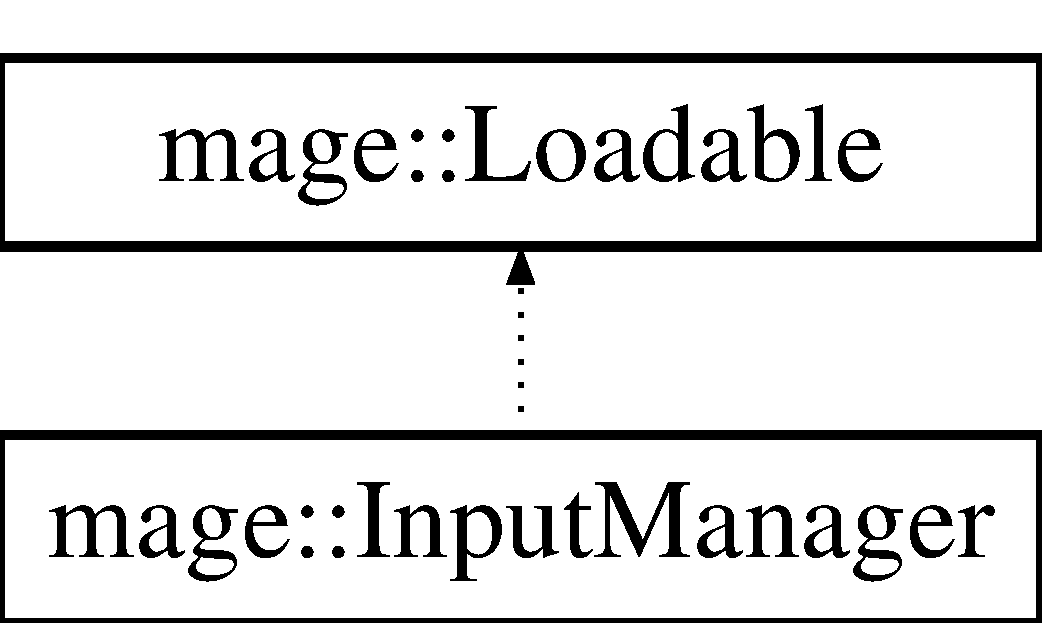
\includegraphics[height=2.000000cm]{classmage_1_1_input_manager}
\end{center}
\end{figure}
\subsection*{Public Member Functions}
\begin{DoxyCompactItemize}
\item 
\hyperlink{classmage_1_1_input_manager_afc28df27a0251c242113a9761c007534}{Input\+Manager} (H\+W\+ND hwindow)
\item 
virtual \hyperlink{classmage_1_1_input_manager_a6e6e612b3b2bacb4ee5d0fcfde35a275}{$\sim$\+Input\+Manager} ()=default
\item 
void \hyperlink{classmage_1_1_input_manager_a5e516969ff4ae9876b98c28f48f93726}{Update} ()
\item 
H\+W\+ND \hyperlink{classmage_1_1_input_manager_a25d5f7f06b1c9d252d44d476f04b5ce3}{Get\+Handle} () const
\item 
const \hyperlink{classmage_1_1_keyboard}{Keyboard} \& \hyperlink{classmage_1_1_input_manager_a1702868136ae35014f27357b5b0f5ce8}{Get\+Keyboard} () const
\item 
const \hyperlink{classmage_1_1_mouse}{Mouse} \& \hyperlink{classmage_1_1_input_manager_a79f8294128ccd710ad80571483377067}{Get\+Mouse} () const
\end{DoxyCompactItemize}
\subsection*{Private Member Functions}
\begin{DoxyCompactItemize}
\item 
\hyperlink{classmage_1_1_input_manager_a68503617f418bf270dc39bb18019b46d}{Input\+Manager} (const \hyperlink{classmage_1_1_input_manager}{Input\+Manager} \&input\+\_\+manager)=delete
\item 
\hyperlink{classmage_1_1_input_manager}{Input\+Manager} \& \hyperlink{classmage_1_1_input_manager_ad9caa8b7e99a69b774887f342bd5dda0}{operator=} (const \hyperlink{classmage_1_1_input_manager}{Input\+Manager} \&input\+\_\+manager)=delete
\item 
H\+R\+E\+S\+U\+LT \hyperlink{classmage_1_1_input_manager_af3ca0717e37916463cc4f40c7d174b33}{Initialize\+DI} ()
\item 
H\+R\+E\+S\+U\+LT \hyperlink{classmage_1_1_input_manager_a34f114c4c667a4a14ce8236b35d308d8}{Initialize\+Input\+Systems} ()
\end{DoxyCompactItemize}
\subsection*{Private Attributes}
\begin{DoxyCompactItemize}
\item 
H\+W\+ND \hyperlink{classmage_1_1_input_manager_a07a1d3a593bc497c747c6d2e4605a229}{m\+\_\+hwindow}
\item 
\hyperlink{namespacemage_ae74f374780900893caa5555d1031fd79}{Com\+Ptr}$<$ I\+Direct\+Input8 $>$ \hyperlink{classmage_1_1_input_manager_a0ffbd0e68b5bab33c35f310625884f3a}{m\+\_\+di}
\item 
\hyperlink{namespacemage_a8c307fbcc33bce9b7f2aa4c26c3b95cf}{Unique\+Ptr}$<$ \hyperlink{classmage_1_1_keyboard}{Keyboard} $>$ \hyperlink{classmage_1_1_input_manager_a196bdd04e169e89d0fa5f6a4a180e4cb}{m\+\_\+keyboard}
\item 
\hyperlink{namespacemage_a8c307fbcc33bce9b7f2aa4c26c3b95cf}{Unique\+Ptr}$<$ \hyperlink{classmage_1_1_mouse}{Mouse} $>$ \hyperlink{classmage_1_1_input_manager_aab9773cccf9626a7e2acb99227b42e37}{m\+\_\+mouse}
\end{DoxyCompactItemize}
\subsection*{Additional Inherited Members}


\subsection{Detailed Description}
A class of input managers. 

\subsection{Constructor \& Destructor Documentation}
\hypertarget{classmage_1_1_input_manager_afc28df27a0251c242113a9761c007534}{}\label{classmage_1_1_input_manager_afc28df27a0251c242113a9761c007534} 
\index{mage\+::\+Input\+Manager@{mage\+::\+Input\+Manager}!Input\+Manager@{Input\+Manager}}
\index{Input\+Manager@{Input\+Manager}!mage\+::\+Input\+Manager@{mage\+::\+Input\+Manager}}
\subsubsection{\texorpdfstring{Input\+Manager()}{InputManager()}\hspace{0.1cm}{\footnotesize\ttfamily [1/2]}}
{\footnotesize\ttfamily mage\+::\+Input\+Manager\+::\+Input\+Manager (\begin{DoxyParamCaption}\item[{H\+W\+ND}]{hwindow }\end{DoxyParamCaption})}

Constructs an input manager for the given window handle.


\begin{DoxyParams}[1]{Parameters}
\mbox{\tt in}  & {\em hwindow} & The handle of the parent window. \\
\hline
\end{DoxyParams}
\hypertarget{classmage_1_1_input_manager_a6e6e612b3b2bacb4ee5d0fcfde35a275}{}\label{classmage_1_1_input_manager_a6e6e612b3b2bacb4ee5d0fcfde35a275} 
\index{mage\+::\+Input\+Manager@{mage\+::\+Input\+Manager}!````~Input\+Manager@{$\sim$\+Input\+Manager}}
\index{````~Input\+Manager@{$\sim$\+Input\+Manager}!mage\+::\+Input\+Manager@{mage\+::\+Input\+Manager}}
\subsubsection{\texorpdfstring{$\sim$\+Input\+Manager()}{~InputManager()}}
{\footnotesize\ttfamily virtual mage\+::\+Input\+Manager\+::$\sim$\+Input\+Manager (\begin{DoxyParamCaption}{ }\end{DoxyParamCaption})\hspace{0.3cm}{\ttfamily [virtual]}, {\ttfamily [default]}}

Destructs this input manager. \hypertarget{classmage_1_1_input_manager_a68503617f418bf270dc39bb18019b46d}{}\label{classmage_1_1_input_manager_a68503617f418bf270dc39bb18019b46d} 
\index{mage\+::\+Input\+Manager@{mage\+::\+Input\+Manager}!Input\+Manager@{Input\+Manager}}
\index{Input\+Manager@{Input\+Manager}!mage\+::\+Input\+Manager@{mage\+::\+Input\+Manager}}
\subsubsection{\texorpdfstring{Input\+Manager()}{InputManager()}\hspace{0.1cm}{\footnotesize\ttfamily [2/2]}}
{\footnotesize\ttfamily mage\+::\+Input\+Manager\+::\+Input\+Manager (\begin{DoxyParamCaption}\item[{const \hyperlink{classmage_1_1_input_manager}{Input\+Manager} \&}]{input\+\_\+manager }\end{DoxyParamCaption})\hspace{0.3cm}{\ttfamily [private]}, {\ttfamily [delete]}}

Constructs an input manager from the given input manager.


\begin{DoxyParams}[1]{Parameters}
\mbox{\tt in}  & {\em input\+\_\+manager} & A reference to the input manager. \\
\hline
\end{DoxyParams}


\subsection{Member Function Documentation}
\hypertarget{classmage_1_1_input_manager_a25d5f7f06b1c9d252d44d476f04b5ce3}{}\label{classmage_1_1_input_manager_a25d5f7f06b1c9d252d44d476f04b5ce3} 
\index{mage\+::\+Input\+Manager@{mage\+::\+Input\+Manager}!Get\+Handle@{Get\+Handle}}
\index{Get\+Handle@{Get\+Handle}!mage\+::\+Input\+Manager@{mage\+::\+Input\+Manager}}
\subsubsection{\texorpdfstring{Get\+Handle()}{GetHandle()}}
{\footnotesize\ttfamily H\+W\+ND mage\+::\+Input\+Manager\+::\+Get\+Handle (\begin{DoxyParamCaption}{ }\end{DoxyParamCaption}) const}

Returns the window handle of this input manager.

\begin{DoxyReturn}{Returns}
The window handle of this input manager. 
\end{DoxyReturn}
\hypertarget{classmage_1_1_input_manager_a1702868136ae35014f27357b5b0f5ce8}{}\label{classmage_1_1_input_manager_a1702868136ae35014f27357b5b0f5ce8} 
\index{mage\+::\+Input\+Manager@{mage\+::\+Input\+Manager}!Get\+Keyboard@{Get\+Keyboard}}
\index{Get\+Keyboard@{Get\+Keyboard}!mage\+::\+Input\+Manager@{mage\+::\+Input\+Manager}}
\subsubsection{\texorpdfstring{Get\+Keyboard()}{GetKeyboard()}}
{\footnotesize\ttfamily const \hyperlink{classmage_1_1_keyboard}{Keyboard}\& mage\+::\+Input\+Manager\+::\+Get\+Keyboard (\begin{DoxyParamCaption}{ }\end{DoxyParamCaption}) const}

Returns the keyboard of this input manager.

\begin{DoxyReturn}{Returns}
A reference to the keyboard of this input manager. 
\end{DoxyReturn}
\hypertarget{classmage_1_1_input_manager_a79f8294128ccd710ad80571483377067}{}\label{classmage_1_1_input_manager_a79f8294128ccd710ad80571483377067} 
\index{mage\+::\+Input\+Manager@{mage\+::\+Input\+Manager}!Get\+Mouse@{Get\+Mouse}}
\index{Get\+Mouse@{Get\+Mouse}!mage\+::\+Input\+Manager@{mage\+::\+Input\+Manager}}
\subsubsection{\texorpdfstring{Get\+Mouse()}{GetMouse()}}
{\footnotesize\ttfamily const \hyperlink{classmage_1_1_mouse}{Mouse}\& mage\+::\+Input\+Manager\+::\+Get\+Mouse (\begin{DoxyParamCaption}{ }\end{DoxyParamCaption}) const}

Returns the mouse of this input manager.

\begin{DoxyReturn}{Returns}
A reference to the mouse of this input manager. 
\end{DoxyReturn}
\hypertarget{classmage_1_1_input_manager_af3ca0717e37916463cc4f40c7d174b33}{}\label{classmage_1_1_input_manager_af3ca0717e37916463cc4f40c7d174b33} 
\index{mage\+::\+Input\+Manager@{mage\+::\+Input\+Manager}!Initialize\+DI@{Initialize\+DI}}
\index{Initialize\+DI@{Initialize\+DI}!mage\+::\+Input\+Manager@{mage\+::\+Input\+Manager}}
\subsubsection{\texorpdfstring{Initialize\+D\+I()}{InitializeDI()}}
{\footnotesize\ttfamily H\+R\+E\+S\+U\+LT mage\+::\+Input\+Manager\+::\+Initialize\+DI (\begin{DoxyParamCaption}{ }\end{DoxyParamCaption})\hspace{0.3cm}{\ttfamily [private]}}

Initializes the Direct\+Input object of this input manager.

\begin{DoxyReturn}{Returns}
A success/error value. 
\end{DoxyReturn}
\hypertarget{classmage_1_1_input_manager_a34f114c4c667a4a14ce8236b35d308d8}{}\label{classmage_1_1_input_manager_a34f114c4c667a4a14ce8236b35d308d8} 
\index{mage\+::\+Input\+Manager@{mage\+::\+Input\+Manager}!Initialize\+Input\+Systems@{Initialize\+Input\+Systems}}
\index{Initialize\+Input\+Systems@{Initialize\+Input\+Systems}!mage\+::\+Input\+Manager@{mage\+::\+Input\+Manager}}
\subsubsection{\texorpdfstring{Initialize\+Input\+Systems()}{InitializeInputSystems()}}
{\footnotesize\ttfamily H\+R\+E\+S\+U\+LT mage\+::\+Input\+Manager\+::\+Initialize\+Input\+Systems (\begin{DoxyParamCaption}{ }\end{DoxyParamCaption})\hspace{0.3cm}{\ttfamily [private]}}

Initializes the different input systems of this input manager. \hypertarget{classmage_1_1_input_manager_ad9caa8b7e99a69b774887f342bd5dda0}{}\label{classmage_1_1_input_manager_ad9caa8b7e99a69b774887f342bd5dda0} 
\index{mage\+::\+Input\+Manager@{mage\+::\+Input\+Manager}!operator=@{operator=}}
\index{operator=@{operator=}!mage\+::\+Input\+Manager@{mage\+::\+Input\+Manager}}
\subsubsection{\texorpdfstring{operator=()}{operator=()}}
{\footnotesize\ttfamily \hyperlink{classmage_1_1_input_manager}{Input\+Manager}\& mage\+::\+Input\+Manager\+::operator= (\begin{DoxyParamCaption}\item[{const \hyperlink{classmage_1_1_input_manager}{Input\+Manager} \&}]{input\+\_\+manager }\end{DoxyParamCaption})\hspace{0.3cm}{\ttfamily [private]}, {\ttfamily [delete]}}

Copies the given input manager to this input manager.


\begin{DoxyParams}[1]{Parameters}
\mbox{\tt in}  & {\em input\+\_\+manager} & A reference to the input manager to copy from. \\
\hline
\end{DoxyParams}
\begin{DoxyReturn}{Returns}
A reference to the copy of the given input manager (i.\+e. this input manager). 
\end{DoxyReturn}
\hypertarget{classmage_1_1_input_manager_a5e516969ff4ae9876b98c28f48f93726}{}\label{classmage_1_1_input_manager_a5e516969ff4ae9876b98c28f48f93726} 
\index{mage\+::\+Input\+Manager@{mage\+::\+Input\+Manager}!Update@{Update}}
\index{Update@{Update}!mage\+::\+Input\+Manager@{mage\+::\+Input\+Manager}}
\subsubsection{\texorpdfstring{Update()}{Update()}}
{\footnotesize\ttfamily void mage\+::\+Input\+Manager\+::\+Update (\begin{DoxyParamCaption}{ }\end{DoxyParamCaption})}

Updates the state of the input systems of this input manager. 

\subsection{Member Data Documentation}
\hypertarget{classmage_1_1_input_manager_a0ffbd0e68b5bab33c35f310625884f3a}{}\label{classmage_1_1_input_manager_a0ffbd0e68b5bab33c35f310625884f3a} 
\index{mage\+::\+Input\+Manager@{mage\+::\+Input\+Manager}!m\+\_\+di@{m\+\_\+di}}
\index{m\+\_\+di@{m\+\_\+di}!mage\+::\+Input\+Manager@{mage\+::\+Input\+Manager}}
\subsubsection{\texorpdfstring{m\+\_\+di}{m\_di}}
{\footnotesize\ttfamily \hyperlink{namespacemage_ae74f374780900893caa5555d1031fd79}{Com\+Ptr}$<$ I\+Direct\+Input8 $>$ mage\+::\+Input\+Manager\+::m\+\_\+di\hspace{0.3cm}{\ttfamily [private]}}

The Direct\+Input object of this input manager.

The methods of the I\+Direct\+Input8 interface are used to enumerate, create, and retrieve the status of Microsoft Direct\+Input device. \hypertarget{classmage_1_1_input_manager_a07a1d3a593bc497c747c6d2e4605a229}{}\label{classmage_1_1_input_manager_a07a1d3a593bc497c747c6d2e4605a229} 
\index{mage\+::\+Input\+Manager@{mage\+::\+Input\+Manager}!m\+\_\+hwindow@{m\+\_\+hwindow}}
\index{m\+\_\+hwindow@{m\+\_\+hwindow}!mage\+::\+Input\+Manager@{mage\+::\+Input\+Manager}}
\subsubsection{\texorpdfstring{m\+\_\+hwindow}{m\_hwindow}}
{\footnotesize\ttfamily H\+W\+ND mage\+::\+Input\+Manager\+::m\+\_\+hwindow\hspace{0.3cm}{\ttfamily [private]}}

The handle of the parent window. \hypertarget{classmage_1_1_input_manager_a196bdd04e169e89d0fa5f6a4a180e4cb}{}\label{classmage_1_1_input_manager_a196bdd04e169e89d0fa5f6a4a180e4cb} 
\index{mage\+::\+Input\+Manager@{mage\+::\+Input\+Manager}!m\+\_\+keyboard@{m\+\_\+keyboard}}
\index{m\+\_\+keyboard@{m\+\_\+keyboard}!mage\+::\+Input\+Manager@{mage\+::\+Input\+Manager}}
\subsubsection{\texorpdfstring{m\+\_\+keyboard}{m\_keyboard}}
{\footnotesize\ttfamily \hyperlink{namespacemage_a8c307fbcc33bce9b7f2aa4c26c3b95cf}{Unique\+Ptr}$<$ \hyperlink{classmage_1_1_keyboard}{Keyboard} $>$ mage\+::\+Input\+Manager\+::m\+\_\+keyboard\hspace{0.3cm}{\ttfamily [private]}}

A pointer to the keyboard of this input manager. \hypertarget{classmage_1_1_input_manager_aab9773cccf9626a7e2acb99227b42e37}{}\label{classmage_1_1_input_manager_aab9773cccf9626a7e2acb99227b42e37} 
\index{mage\+::\+Input\+Manager@{mage\+::\+Input\+Manager}!m\+\_\+mouse@{m\+\_\+mouse}}
\index{m\+\_\+mouse@{m\+\_\+mouse}!mage\+::\+Input\+Manager@{mage\+::\+Input\+Manager}}
\subsubsection{\texorpdfstring{m\+\_\+mouse}{m\_mouse}}
{\footnotesize\ttfamily \hyperlink{namespacemage_a8c307fbcc33bce9b7f2aa4c26c3b95cf}{Unique\+Ptr}$<$ \hyperlink{classmage_1_1_mouse}{Mouse} $>$ mage\+::\+Input\+Manager\+::m\+\_\+mouse\hspace{0.3cm}{\ttfamily [private]}}

A pointer to the mouse of this input manager. 
\hypertarget{classmage_1_1_keyboard}{}\section{mage\+:\+:Keyboard Class Reference}
\label{classmage_1_1_keyboard}\index{mage\+::\+Keyboard@{mage\+::\+Keyboard}}


{\ttfamily \#include $<$keyboard.\+hpp$>$}

Inheritance diagram for mage\+:\+:Keyboard\+:\begin{figure}[H]
\begin{center}
\leavevmode
\includegraphics[height=2.000000cm]{classmage_1_1_keyboard}
\end{center}
\end{figure}
\subsection*{Public Member Functions}
\begin{DoxyCompactItemize}
\item 
\hyperlink{classmage_1_1_keyboard_af4afb6c7992b88f94f4b310c35f7e867}{Keyboard} (H\+W\+ND hwindow, \hyperlink{namespacemage_ae74f374780900893caa5555d1031fd79}{Com\+Ptr}$<$ I\+Direct\+Input8 $>$ di)
\item 
virtual \hyperlink{classmage_1_1_keyboard_a72426c8e5cd32f8e79f283d5409f9cc4}{$\sim$\+Keyboard} ()=default
\item 
void \hyperlink{classmage_1_1_keyboard_abb5fd91a304f8bbf8b15ab1a277dafaf}{Update} ()
\item 
H\+W\+ND \hyperlink{classmage_1_1_keyboard_ab9d2244f94faccb9c745b07a8bebc888}{Get\+Handle} () const
\item 
bool \hyperlink{classmage_1_1_keyboard_a94d35ad5ad27e3fc9496f3ab1fa28e4d}{Get\+Key\+Press} (unsigned char key, bool ignore\+\_\+press\+\_\+stamp=false) const
\end{DoxyCompactItemize}
\subsection*{Private Member Functions}
\begin{DoxyCompactItemize}
\item 
\hyperlink{classmage_1_1_keyboard_a39d07f8a5e37648ca9eba30aa55146bf}{Keyboard} (const \hyperlink{classmage_1_1_keyboard}{Keyboard} \&keyboard)=delete
\item 
\hyperlink{classmage_1_1_keyboard}{Keyboard} \& \hyperlink{classmage_1_1_keyboard_ae3ba98190c8c14ea894c676888825f35}{operator=} (const \hyperlink{classmage_1_1_keyboard}{Keyboard} \&keyboard)=delete
\item 
H\+R\+E\+S\+U\+LT \hyperlink{classmage_1_1_keyboard_a1d3211c7377529e570bb5cde900f73db}{Initialize\+Keyboard} (\hyperlink{namespacemage_ae74f374780900893caa5555d1031fd79}{Com\+Ptr}$<$ I\+Direct\+Input8 $>$ di)
\end{DoxyCompactItemize}
\subsection*{Private Attributes}
\begin{DoxyCompactItemize}
\item 
H\+W\+ND \hyperlink{classmage_1_1_keyboard_aa7196c689dad6f5aaf35e3929de02791}{m\+\_\+hwindow}
\item 
\hyperlink{namespacemage_ae74f374780900893caa5555d1031fd79}{Com\+Ptr}$<$ I\+Direct\+Input\+Device8 $>$ \hyperlink{classmage_1_1_keyboard_a992b8b8caf0d858163e5e9af04302324}{m\+\_\+keyboard}
\item 
uint64\+\_\+t \hyperlink{classmage_1_1_keyboard_a2c638a93d1f61d9d3578a0df8b6a1c39}{m\+\_\+press\+\_\+stamp}
\item 
unsigned char \hyperlink{classmage_1_1_keyboard_a7499df459499f5addd50507ea1e2358c}{m\+\_\+key\+\_\+state} \mbox{[}256\mbox{]}
\item 
uint64\+\_\+t \hyperlink{classmage_1_1_keyboard_a8eb4ce7e4e2395bb27d2ac9236655335}{m\+\_\+key\+\_\+press\+\_\+stamp} \mbox{[}256\mbox{]}
\end{DoxyCompactItemize}
\subsection*{Additional Inherited Members}


\subsection{Detailed Description}
A class of keyboards. 

\subsection{Constructor \& Destructor Documentation}
\hypertarget{classmage_1_1_keyboard_af4afb6c7992b88f94f4b310c35f7e867}{}\label{classmage_1_1_keyboard_af4afb6c7992b88f94f4b310c35f7e867} 
\index{mage\+::\+Keyboard@{mage\+::\+Keyboard}!Keyboard@{Keyboard}}
\index{Keyboard@{Keyboard}!mage\+::\+Keyboard@{mage\+::\+Keyboard}}
\subsubsection{\texorpdfstring{Keyboard()}{Keyboard()}\hspace{0.1cm}{\footnotesize\ttfamily [1/2]}}
{\footnotesize\ttfamily mage\+::\+Keyboard\+::\+Keyboard (\begin{DoxyParamCaption}\item[{H\+W\+ND}]{hwindow,  }\item[{\hyperlink{namespacemage_ae74f374780900893caa5555d1031fd79}{Com\+Ptr}$<$ I\+Direct\+Input8 $>$}]{di }\end{DoxyParamCaption})}

Constructs a keyboard.


\begin{DoxyParams}[1]{Parameters}
\mbox{\tt in}  & {\em hwindow} & The handle of the parent window. \\
\hline
\mbox{\tt in}  & {\em di} & A pointer to a direct input object. \\
\hline
\end{DoxyParams}
\hypertarget{classmage_1_1_keyboard_a72426c8e5cd32f8e79f283d5409f9cc4}{}\label{classmage_1_1_keyboard_a72426c8e5cd32f8e79f283d5409f9cc4} 
\index{mage\+::\+Keyboard@{mage\+::\+Keyboard}!````~Keyboard@{$\sim$\+Keyboard}}
\index{````~Keyboard@{$\sim$\+Keyboard}!mage\+::\+Keyboard@{mage\+::\+Keyboard}}
\subsubsection{\texorpdfstring{$\sim$\+Keyboard()}{~Keyboard()}}
{\footnotesize\ttfamily virtual mage\+::\+Keyboard\+::$\sim$\+Keyboard (\begin{DoxyParamCaption}{ }\end{DoxyParamCaption})\hspace{0.3cm}{\ttfamily [virtual]}, {\ttfamily [default]}}

Destructs this keyboard. \hypertarget{classmage_1_1_keyboard_a39d07f8a5e37648ca9eba30aa55146bf}{}\label{classmage_1_1_keyboard_a39d07f8a5e37648ca9eba30aa55146bf} 
\index{mage\+::\+Keyboard@{mage\+::\+Keyboard}!Keyboard@{Keyboard}}
\index{Keyboard@{Keyboard}!mage\+::\+Keyboard@{mage\+::\+Keyboard}}
\subsubsection{\texorpdfstring{Keyboard()}{Keyboard()}\hspace{0.1cm}{\footnotesize\ttfamily [2/2]}}
{\footnotesize\ttfamily mage\+::\+Keyboard\+::\+Keyboard (\begin{DoxyParamCaption}\item[{const \hyperlink{classmage_1_1_keyboard}{Keyboard} \&}]{keyboard }\end{DoxyParamCaption})\hspace{0.3cm}{\ttfamily [private]}, {\ttfamily [delete]}}

Constructs a keyboard from the given keyboard.


\begin{DoxyParams}[1]{Parameters}
\mbox{\tt in}  & {\em keyboard} & A reference to the keyboard. \\
\hline
\end{DoxyParams}


\subsection{Member Function Documentation}
\hypertarget{classmage_1_1_keyboard_ab9d2244f94faccb9c745b07a8bebc888}{}\label{classmage_1_1_keyboard_ab9d2244f94faccb9c745b07a8bebc888} 
\index{mage\+::\+Keyboard@{mage\+::\+Keyboard}!Get\+Handle@{Get\+Handle}}
\index{Get\+Handle@{Get\+Handle}!mage\+::\+Keyboard@{mage\+::\+Keyboard}}
\subsubsection{\texorpdfstring{Get\+Handle()}{GetHandle()}}
{\footnotesize\ttfamily H\+W\+ND mage\+::\+Keyboard\+::\+Get\+Handle (\begin{DoxyParamCaption}{ }\end{DoxyParamCaption}) const}

Returns the window handle of this keyboard.

\begin{DoxyReturn}{Returns}
The window handle of this keyboard. 
\end{DoxyReturn}
\hypertarget{classmage_1_1_keyboard_a94d35ad5ad27e3fc9496f3ab1fa28e4d}{}\label{classmage_1_1_keyboard_a94d35ad5ad27e3fc9496f3ab1fa28e4d} 
\index{mage\+::\+Keyboard@{mage\+::\+Keyboard}!Get\+Key\+Press@{Get\+Key\+Press}}
\index{Get\+Key\+Press@{Get\+Key\+Press}!mage\+::\+Keyboard@{mage\+::\+Keyboard}}
\subsubsection{\texorpdfstring{Get\+Key\+Press()}{GetKeyPress()}}
{\footnotesize\ttfamily bool mage\+::\+Keyboard\+::\+Get\+Key\+Press (\begin{DoxyParamCaption}\item[{unsigned char}]{key,  }\item[{bool}]{ignore\+\_\+press\+\_\+stamp = {\ttfamily false} }\end{DoxyParamCaption}) const}

Checks whether the given key of this keyboard is pressed.


\begin{DoxyParams}[1]{Parameters}
\mbox{\tt in}  & {\em key} & The key. \\
\hline
\mbox{\tt in}  & {\em ignore\+\_\+press\+\_\+stamp} & Flag indicating whether press stamps should be ignored. Consistent presses will return false when using the press stamp. \\
\hline
\end{DoxyParams}
\begin{DoxyReturn}{Returns}
{\ttfamily true} if the given key of this keyboard is pressed. {\ttfamily false} otherwise. 
\end{DoxyReturn}
\hypertarget{classmage_1_1_keyboard_a1d3211c7377529e570bb5cde900f73db}{}\label{classmage_1_1_keyboard_a1d3211c7377529e570bb5cde900f73db} 
\index{mage\+::\+Keyboard@{mage\+::\+Keyboard}!Initialize\+Keyboard@{Initialize\+Keyboard}}
\index{Initialize\+Keyboard@{Initialize\+Keyboard}!mage\+::\+Keyboard@{mage\+::\+Keyboard}}
\subsubsection{\texorpdfstring{Initialize\+Keyboard()}{InitializeKeyboard()}}
{\footnotesize\ttfamily H\+R\+E\+S\+U\+LT mage\+::\+Keyboard\+::\+Initialize\+Keyboard (\begin{DoxyParamCaption}\item[{\hyperlink{namespacemage_ae74f374780900893caa5555d1031fd79}{Com\+Ptr}$<$ I\+Direct\+Input8 $>$}]{di }\end{DoxyParamCaption})\hspace{0.3cm}{\ttfamily [private]}}

Initializes the keyboard device of this keyboard.


\begin{DoxyParams}[1]{Parameters}
\mbox{\tt in}  & {\em di} & A pointer to a direct input object. \\
\hline
\end{DoxyParams}
\begin{DoxyReturn}{Returns}
A success/error value. 
\end{DoxyReturn}
\hypertarget{classmage_1_1_keyboard_ae3ba98190c8c14ea894c676888825f35}{}\label{classmage_1_1_keyboard_ae3ba98190c8c14ea894c676888825f35} 
\index{mage\+::\+Keyboard@{mage\+::\+Keyboard}!operator=@{operator=}}
\index{operator=@{operator=}!mage\+::\+Keyboard@{mage\+::\+Keyboard}}
\subsubsection{\texorpdfstring{operator=()}{operator=()}}
{\footnotesize\ttfamily \hyperlink{classmage_1_1_keyboard}{Keyboard}\& mage\+::\+Keyboard\+::operator= (\begin{DoxyParamCaption}\item[{const \hyperlink{classmage_1_1_keyboard}{Keyboard} \&}]{keyboard }\end{DoxyParamCaption})\hspace{0.3cm}{\ttfamily [private]}, {\ttfamily [delete]}}

Copies the given keyboard to this keyboard.


\begin{DoxyParams}[1]{Parameters}
\mbox{\tt in}  & {\em keyboard} & A reference to the keyboard to copy from. \\
\hline
\end{DoxyParams}
\begin{DoxyReturn}{Returns}
A reference to the copy of the given keyboard (i.\+e. this keyboard). 
\end{DoxyReturn}
\hypertarget{classmage_1_1_keyboard_abb5fd91a304f8bbf8b15ab1a277dafaf}{}\label{classmage_1_1_keyboard_abb5fd91a304f8bbf8b15ab1a277dafaf} 
\index{mage\+::\+Keyboard@{mage\+::\+Keyboard}!Update@{Update}}
\index{Update@{Update}!mage\+::\+Keyboard@{mage\+::\+Keyboard}}
\subsubsection{\texorpdfstring{Update()}{Update()}}
{\footnotesize\ttfamily void mage\+::\+Keyboard\+::\+Update (\begin{DoxyParamCaption}{ }\end{DoxyParamCaption})}

Updates the state of this keyboard. 

\subsection{Member Data Documentation}
\hypertarget{classmage_1_1_keyboard_aa7196c689dad6f5aaf35e3929de02791}{}\label{classmage_1_1_keyboard_aa7196c689dad6f5aaf35e3929de02791} 
\index{mage\+::\+Keyboard@{mage\+::\+Keyboard}!m\+\_\+hwindow@{m\+\_\+hwindow}}
\index{m\+\_\+hwindow@{m\+\_\+hwindow}!mage\+::\+Keyboard@{mage\+::\+Keyboard}}
\subsubsection{\texorpdfstring{m\+\_\+hwindow}{m\_hwindow}}
{\footnotesize\ttfamily H\+W\+ND mage\+::\+Keyboard\+::m\+\_\+hwindow\hspace{0.3cm}{\ttfamily [private]}}

The handle of the parent window. \hypertarget{classmage_1_1_keyboard_a8eb4ce7e4e2395bb27d2ac9236655335}{}\label{classmage_1_1_keyboard_a8eb4ce7e4e2395bb27d2ac9236655335} 
\index{mage\+::\+Keyboard@{mage\+::\+Keyboard}!m\+\_\+key\+\_\+press\+\_\+stamp@{m\+\_\+key\+\_\+press\+\_\+stamp}}
\index{m\+\_\+key\+\_\+press\+\_\+stamp@{m\+\_\+key\+\_\+press\+\_\+stamp}!mage\+::\+Keyboard@{mage\+::\+Keyboard}}
\subsubsection{\texorpdfstring{m\+\_\+key\+\_\+press\+\_\+stamp}{m\_key\_press\_stamp}}
{\footnotesize\ttfamily uint64\+\_\+t mage\+::\+Keyboard\+::m\+\_\+key\+\_\+press\+\_\+stamp\mbox{[}256\mbox{]}\hspace{0.3cm}{\ttfamily [mutable]}, {\ttfamily [private]}}

Stamps the keys pressed in the last frame of this keyboard. \hypertarget{classmage_1_1_keyboard_a7499df459499f5addd50507ea1e2358c}{}\label{classmage_1_1_keyboard_a7499df459499f5addd50507ea1e2358c} 
\index{mage\+::\+Keyboard@{mage\+::\+Keyboard}!m\+\_\+key\+\_\+state@{m\+\_\+key\+\_\+state}}
\index{m\+\_\+key\+\_\+state@{m\+\_\+key\+\_\+state}!mage\+::\+Keyboard@{mage\+::\+Keyboard}}
\subsubsection{\texorpdfstring{m\+\_\+key\+\_\+state}{m\_key\_state}}
{\footnotesize\ttfamily unsigned char mage\+::\+Keyboard\+::m\+\_\+key\+\_\+state\mbox{[}256\mbox{]}\hspace{0.3cm}{\ttfamily [private]}}

State of the keys of this keyboard. \hypertarget{classmage_1_1_keyboard_a992b8b8caf0d858163e5e9af04302324}{}\label{classmage_1_1_keyboard_a992b8b8caf0d858163e5e9af04302324} 
\index{mage\+::\+Keyboard@{mage\+::\+Keyboard}!m\+\_\+keyboard@{m\+\_\+keyboard}}
\index{m\+\_\+keyboard@{m\+\_\+keyboard}!mage\+::\+Keyboard@{mage\+::\+Keyboard}}
\subsubsection{\texorpdfstring{m\+\_\+keyboard}{m\_keyboard}}
{\footnotesize\ttfamily \hyperlink{namespacemage_ae74f374780900893caa5555d1031fd79}{Com\+Ptr}$<$ I\+Direct\+Input\+Device8 $>$ mage\+::\+Keyboard\+::m\+\_\+keyboard\hspace{0.3cm}{\ttfamily [private]}}

The Direct\+Input keyboard device of this keyboard.

The methods of the I\+Direct\+Input\+Device8 interface are used to gain and release access to Microsoft Direct\+Input devices, manage device properties and information, set behavior, perform initialization, create and play force-\/feedback effects, and invoke a device\textquotesingle{}s control panel. \hypertarget{classmage_1_1_keyboard_a2c638a93d1f61d9d3578a0df8b6a1c39}{}\label{classmage_1_1_keyboard_a2c638a93d1f61d9d3578a0df8b6a1c39} 
\index{mage\+::\+Keyboard@{mage\+::\+Keyboard}!m\+\_\+press\+\_\+stamp@{m\+\_\+press\+\_\+stamp}}
\index{m\+\_\+press\+\_\+stamp@{m\+\_\+press\+\_\+stamp}!mage\+::\+Keyboard@{mage\+::\+Keyboard}}
\subsubsection{\texorpdfstring{m\+\_\+press\+\_\+stamp}{m\_press\_stamp}}
{\footnotesize\ttfamily uint64\+\_\+t mage\+::\+Keyboard\+::m\+\_\+press\+\_\+stamp\hspace{0.3cm}{\ttfamily [private]}}

The current press stamp (incremented every frame). 
\hypertarget{classmage_1_1_loadable}{}\section{mage\+:\+:Loadable Class Reference}
\label{classmage_1_1_loadable}\index{mage\+::\+Loadable@{mage\+::\+Loadable}}


{\ttfamily \#include $<$loadable.\+hpp$>$}

Inheritance diagram for mage\+:\+:Loadable\+:\begin{figure}[H]
\begin{center}
\leavevmode
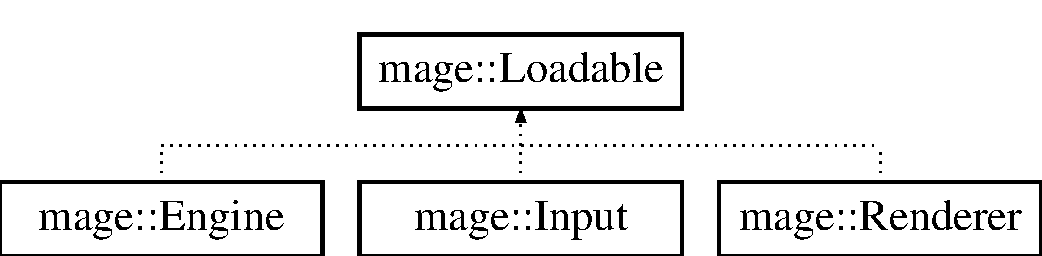
\includegraphics[height=1.393035cm]{classmage_1_1_loadable}
\end{center}
\end{figure}
\subsection*{Public Member Functions}
\begin{DoxyCompactItemize}
\item 
bool \hyperlink{classmage_1_1_loadable_a53cfa5beb9b44bbcda0d6166a54b8cb6}{Is\+Loaded} () const
\end{DoxyCompactItemize}
\subsection*{Protected Member Functions}
\begin{DoxyCompactItemize}
\item 
\hyperlink{classmage_1_1_loadable_afbdcb287b5e20583899a27a1c244bc7d}{Loadable} (bool loaded=false)
\item 
\hyperlink{classmage_1_1_loadable_a21364449c045d579cb6090347d83cd54}{Loadable} (const \hyperlink{classmage_1_1_loadable}{Loadable} \&loadable)=default
\item 
virtual \hyperlink{classmage_1_1_loadable_a7f51b5e1065ebe4dd1da7ef9c9966546}{$\sim$\+Loadable} ()=default
\item 
\hyperlink{classmage_1_1_loadable}{Loadable} \& \hyperlink{classmage_1_1_loadable_a82277616525b6ed9b1e19fd2dcdb4c0d}{operator=} (const \hyperlink{classmage_1_1_loadable}{Loadable} \&loadable)=default
\item 
void \hyperlink{classmage_1_1_loadable_a932ff8b287c8e68e30a13804cba08ff2}{Set\+Loaded} (bool loaded=true)
\end{DoxyCompactItemize}
\subsection*{Private Attributes}
\begin{DoxyCompactItemize}
\item 
bool \hyperlink{classmage_1_1_loadable_a993963fbfeb0f2e2ab9616bf7ef6a0f7}{m\+\_\+loaded}
\end{DoxyCompactItemize}


\subsection{Detailed Description}
A class of loadables. 

\subsection{Constructor \& Destructor Documentation}
\hypertarget{classmage_1_1_loadable_afbdcb287b5e20583899a27a1c244bc7d}{}\label{classmage_1_1_loadable_afbdcb287b5e20583899a27a1c244bc7d} 
\index{mage\+::\+Loadable@{mage\+::\+Loadable}!Loadable@{Loadable}}
\index{Loadable@{Loadable}!mage\+::\+Loadable@{mage\+::\+Loadable}}
\subsubsection{\texorpdfstring{Loadable()}{Loadable()}\hspace{0.1cm}{\footnotesize\ttfamily [1/2]}}
{\footnotesize\ttfamily mage\+::\+Loadable\+::\+Loadable (\begin{DoxyParamCaption}\item[{bool}]{loaded = {\ttfamily false} }\end{DoxyParamCaption})\hspace{0.3cm}{\ttfamily [protected]}}

Constructs a loadable.


\begin{DoxyParams}[1]{Parameters}
\mbox{\tt in}  & {\em loaded} & Flag indicating wether the loadable is loaded. \\
\hline
\end{DoxyParams}
\hypertarget{classmage_1_1_loadable_a21364449c045d579cb6090347d83cd54}{}\label{classmage_1_1_loadable_a21364449c045d579cb6090347d83cd54} 
\index{mage\+::\+Loadable@{mage\+::\+Loadable}!Loadable@{Loadable}}
\index{Loadable@{Loadable}!mage\+::\+Loadable@{mage\+::\+Loadable}}
\subsubsection{\texorpdfstring{Loadable()}{Loadable()}\hspace{0.1cm}{\footnotesize\ttfamily [2/2]}}
{\footnotesize\ttfamily mage\+::\+Loadable\+::\+Loadable (\begin{DoxyParamCaption}\item[{const \hyperlink{classmage_1_1_loadable}{Loadable} \&}]{loadable }\end{DoxyParamCaption})\hspace{0.3cm}{\ttfamily [protected]}, {\ttfamily [default]}}

Constructs a loadable from the given loadable.


\begin{DoxyParams}[1]{Parameters}
\mbox{\tt in}  & {\em loadable} & A reference to the loadable. \\
\hline
\end{DoxyParams}
\hypertarget{classmage_1_1_loadable_a7f51b5e1065ebe4dd1da7ef9c9966546}{}\label{classmage_1_1_loadable_a7f51b5e1065ebe4dd1da7ef9c9966546} 
\index{mage\+::\+Loadable@{mage\+::\+Loadable}!````~Loadable@{$\sim$\+Loadable}}
\index{````~Loadable@{$\sim$\+Loadable}!mage\+::\+Loadable@{mage\+::\+Loadable}}
\subsubsection{\texorpdfstring{$\sim$\+Loadable()}{~Loadable()}}
{\footnotesize\ttfamily virtual mage\+::\+Loadable\+::$\sim$\+Loadable (\begin{DoxyParamCaption}{ }\end{DoxyParamCaption})\hspace{0.3cm}{\ttfamily [protected]}, {\ttfamily [virtual]}, {\ttfamily [default]}}

Destructs this loadable. 

\subsection{Member Function Documentation}
\hypertarget{classmage_1_1_loadable_a53cfa5beb9b44bbcda0d6166a54b8cb6}{}\label{classmage_1_1_loadable_a53cfa5beb9b44bbcda0d6166a54b8cb6} 
\index{mage\+::\+Loadable@{mage\+::\+Loadable}!Is\+Loaded@{Is\+Loaded}}
\index{Is\+Loaded@{Is\+Loaded}!mage\+::\+Loadable@{mage\+::\+Loadable}}
\subsubsection{\texorpdfstring{Is\+Loaded()}{IsLoaded()}}
{\footnotesize\ttfamily bool mage\+::\+Loadable\+::\+Is\+Loaded (\begin{DoxyParamCaption}{ }\end{DoxyParamCaption}) const}

Checks wether this loadable is loaded.

\begin{DoxyReturn}{Returns}
{\ttfamily true} if this loadable is loaded. {\ttfamily false} otherwise. 
\end{DoxyReturn}
\hypertarget{classmage_1_1_loadable_a82277616525b6ed9b1e19fd2dcdb4c0d}{}\label{classmage_1_1_loadable_a82277616525b6ed9b1e19fd2dcdb4c0d} 
\index{mage\+::\+Loadable@{mage\+::\+Loadable}!operator=@{operator=}}
\index{operator=@{operator=}!mage\+::\+Loadable@{mage\+::\+Loadable}}
\subsubsection{\texorpdfstring{operator=()}{operator=()}}
{\footnotesize\ttfamily \hyperlink{classmage_1_1_loadable}{Loadable}\& mage\+::\+Loadable\+::operator= (\begin{DoxyParamCaption}\item[{const \hyperlink{classmage_1_1_loadable}{Loadable} \&}]{loadable }\end{DoxyParamCaption})\hspace{0.3cm}{\ttfamily [protected]}, {\ttfamily [default]}}

Copies the given loadable to this loadable.


\begin{DoxyParams}[1]{Parameters}
\mbox{\tt in}  & {\em loadable} & A reference to the loadable to copy from. \\
\hline
\end{DoxyParams}
\begin{DoxyReturn}{Returns}
A reference to the copy of the given loadable (i.\+e. this loadable). 
\end{DoxyReturn}
\hypertarget{classmage_1_1_loadable_a932ff8b287c8e68e30a13804cba08ff2}{}\label{classmage_1_1_loadable_a932ff8b287c8e68e30a13804cba08ff2} 
\index{mage\+::\+Loadable@{mage\+::\+Loadable}!Set\+Loaded@{Set\+Loaded}}
\index{Set\+Loaded@{Set\+Loaded}!mage\+::\+Loadable@{mage\+::\+Loadable}}
\subsubsection{\texorpdfstring{Set\+Loaded()}{SetLoaded()}}
{\footnotesize\ttfamily void mage\+::\+Loadable\+::\+Set\+Loaded (\begin{DoxyParamCaption}\item[{bool}]{loaded = {\ttfamily true} }\end{DoxyParamCaption})\hspace{0.3cm}{\ttfamily [protected]}}

Set the state of this loadable to the given value.


\begin{DoxyParams}[1]{Parameters}
\mbox{\tt in}  & {\em loaded} & Flag indicating wether this loadable is loaded. \\
\hline
\end{DoxyParams}


\subsection{Member Data Documentation}
\hypertarget{classmage_1_1_loadable_a993963fbfeb0f2e2ab9616bf7ef6a0f7}{}\label{classmage_1_1_loadable_a993963fbfeb0f2e2ab9616bf7ef6a0f7} 
\index{mage\+::\+Loadable@{mage\+::\+Loadable}!m\+\_\+loaded@{m\+\_\+loaded}}
\index{m\+\_\+loaded@{m\+\_\+loaded}!mage\+::\+Loadable@{mage\+::\+Loadable}}
\subsubsection{\texorpdfstring{m\+\_\+loaded}{m\_loaded}}
{\footnotesize\ttfamily bool mage\+::\+Loadable\+::m\+\_\+loaded\hspace{0.3cm}{\ttfamily [private]}}

Flag indicating wether this loadable is loaded. 
\hypertarget{structmage_1_1_logging_configuration}{}\section{mage\+:\+:Logging\+Configuration Struct Reference}
\label{structmage_1_1_logging_configuration}\index{mage\+::\+Logging\+Configuration@{mage\+::\+Logging\+Configuration}}


{\ttfamily \#include $<$logging.\+hpp$>$}

\subsection*{Public Member Functions}
\begin{DoxyCompactItemize}
\item 
\hyperlink{structmage_1_1_logging_configuration_a3d397c3ce26c1c42c9ae4a391391c6f9}{Logging\+Configuration} ()
\item 
\hyperlink{structmage_1_1_logging_configuration_afd44a8c35f8c2e2f7d75b876ae504b06}{Logging\+Configuration} (const \hyperlink{structmage_1_1_logging_configuration}{Logging\+Configuration} \&logging\+\_\+configuration)
\item 
\hyperlink{structmage_1_1_logging_configuration_ad00ecf9ceadffac0c35d102f50fbd8c7}{$\sim$\+Logging\+Configuration} ()
\item 
\hyperlink{structmage_1_1_logging_configuration}{Logging\+Configuration} \& \hyperlink{structmage_1_1_logging_configuration_af19880c8b37ae454901a19dccdf4a297}{operator=} (const \hyperlink{structmage_1_1_logging_configuration}{Logging\+Configuration} \&logging\+\_\+configuration)
\item 
bool \hyperlink{structmage_1_1_logging_configuration_ac081313b7a9440bcd73b6a9b69ff3452}{Is\+Quiet} () const
\item 
bool \hyperlink{structmage_1_1_logging_configuration_a13d91de33f888eee31f4d4e6b1237675}{Is\+Verbose} () const
\end{DoxyCompactItemize}
\subsection*{Private Attributes}
\begin{DoxyCompactItemize}
\item 
bool \hyperlink{structmage_1_1_logging_configuration_a38f457d5db84d15e008841ca8653b47c}{m\+\_\+quiet}
\item 
bool \hyperlink{structmage_1_1_logging_configuration_a60f052c2bb702d8153188e93f00427ac}{m\+\_\+verbose}
\end{DoxyCompactItemize}


\subsection{Detailed Description}
A struct of logging configurations of the engine processing. 

\subsection{Constructor \& Destructor Documentation}
\hypertarget{structmage_1_1_logging_configuration_a3d397c3ce26c1c42c9ae4a391391c6f9}{}\label{structmage_1_1_logging_configuration_a3d397c3ce26c1c42c9ae4a391391c6f9} 
\index{mage\+::\+Logging\+Configuration@{mage\+::\+Logging\+Configuration}!Logging\+Configuration@{Logging\+Configuration}}
\index{Logging\+Configuration@{Logging\+Configuration}!mage\+::\+Logging\+Configuration@{mage\+::\+Logging\+Configuration}}
\subsubsection{\texorpdfstring{Logging\+Configuration()}{LoggingConfiguration()}\hspace{0.1cm}{\footnotesize\ttfamily [1/2]}}
{\footnotesize\ttfamily mage\+::\+Logging\+Configuration\+::\+Logging\+Configuration (\begin{DoxyParamCaption}{ }\end{DoxyParamCaption})}

Constructs a new logging configuration. \hypertarget{structmage_1_1_logging_configuration_afd44a8c35f8c2e2f7d75b876ae504b06}{}\label{structmage_1_1_logging_configuration_afd44a8c35f8c2e2f7d75b876ae504b06} 
\index{mage\+::\+Logging\+Configuration@{mage\+::\+Logging\+Configuration}!Logging\+Configuration@{Logging\+Configuration}}
\index{Logging\+Configuration@{Logging\+Configuration}!mage\+::\+Logging\+Configuration@{mage\+::\+Logging\+Configuration}}
\subsubsection{\texorpdfstring{Logging\+Configuration()}{LoggingConfiguration()}\hspace{0.1cm}{\footnotesize\ttfamily [2/2]}}
{\footnotesize\ttfamily mage\+::\+Logging\+Configuration\+::\+Logging\+Configuration (\begin{DoxyParamCaption}\item[{const \hyperlink{structmage_1_1_logging_configuration}{Logging\+Configuration} \&}]{logging\+\_\+configuration }\end{DoxyParamCaption})}

Constructs a logging configuration from the given logging configuration.


\begin{DoxyParams}[1]{Parameters}
\mbox{\tt in}  & {\em logging\+\_\+configuration} & A reference to the logging configuration. \\
\hline
\end{DoxyParams}
\hypertarget{structmage_1_1_logging_configuration_ad00ecf9ceadffac0c35d102f50fbd8c7}{}\label{structmage_1_1_logging_configuration_ad00ecf9ceadffac0c35d102f50fbd8c7} 
\index{mage\+::\+Logging\+Configuration@{mage\+::\+Logging\+Configuration}!````~Logging\+Configuration@{$\sim$\+Logging\+Configuration}}
\index{````~Logging\+Configuration@{$\sim$\+Logging\+Configuration}!mage\+::\+Logging\+Configuration@{mage\+::\+Logging\+Configuration}}
\subsubsection{\texorpdfstring{$\sim$\+Logging\+Configuration()}{~LoggingConfiguration()}}
{\footnotesize\ttfamily mage\+::\+Logging\+Configuration\+::$\sim$\+Logging\+Configuration (\begin{DoxyParamCaption}{ }\end{DoxyParamCaption})}

Destructs this logging configuration. 

\subsection{Member Function Documentation}
\hypertarget{structmage_1_1_logging_configuration_ac081313b7a9440bcd73b6a9b69ff3452}{}\label{structmage_1_1_logging_configuration_ac081313b7a9440bcd73b6a9b69ff3452} 
\index{mage\+::\+Logging\+Configuration@{mage\+::\+Logging\+Configuration}!Is\+Quiet@{Is\+Quiet}}
\index{Is\+Quiet@{Is\+Quiet}!mage\+::\+Logging\+Configuration@{mage\+::\+Logging\+Configuration}}
\subsubsection{\texorpdfstring{Is\+Quiet()}{IsQuiet()}}
{\footnotesize\ttfamily bool mage\+::\+Logging\+Configuration\+::\+Is\+Quiet (\begin{DoxyParamCaption}{ }\end{DoxyParamCaption}) const}

Checks whether the logging of the engine processing is quiet.

\begin{DoxyReturn}{Returns}
{\ttfamily true} if the logging of the engine processing is quiet. {\ttfamily false} otherwise. 
\end{DoxyReturn}
\hypertarget{structmage_1_1_logging_configuration_a13d91de33f888eee31f4d4e6b1237675}{}\label{structmage_1_1_logging_configuration_a13d91de33f888eee31f4d4e6b1237675} 
\index{mage\+::\+Logging\+Configuration@{mage\+::\+Logging\+Configuration}!Is\+Verbose@{Is\+Verbose}}
\index{Is\+Verbose@{Is\+Verbose}!mage\+::\+Logging\+Configuration@{mage\+::\+Logging\+Configuration}}
\subsubsection{\texorpdfstring{Is\+Verbose()}{IsVerbose()}}
{\footnotesize\ttfamily bool mage\+::\+Logging\+Configuration\+::\+Is\+Verbose (\begin{DoxyParamCaption}{ }\end{DoxyParamCaption}) const}

Checks wheter the logging of the engine processing is verbose.

\begin{DoxyReturn}{Returns}
{\ttfamily true} if the logging of the engine processing is verbose. {\ttfamily false} otherwise. 
\end{DoxyReturn}
\hypertarget{structmage_1_1_logging_configuration_af19880c8b37ae454901a19dccdf4a297}{}\label{structmage_1_1_logging_configuration_af19880c8b37ae454901a19dccdf4a297} 
\index{mage\+::\+Logging\+Configuration@{mage\+::\+Logging\+Configuration}!operator=@{operator=}}
\index{operator=@{operator=}!mage\+::\+Logging\+Configuration@{mage\+::\+Logging\+Configuration}}
\subsubsection{\texorpdfstring{operator=()}{operator=()}}
{\footnotesize\ttfamily \hyperlink{structmage_1_1_logging_configuration}{Logging\+Configuration}\& mage\+::\+Logging\+Configuration\+::operator= (\begin{DoxyParamCaption}\item[{const \hyperlink{structmage_1_1_logging_configuration}{Logging\+Configuration} \&}]{logging\+\_\+configuration }\end{DoxyParamCaption})}

Copies the given logging configuration to this logging configuration.


\begin{DoxyParams}[1]{Parameters}
\mbox{\tt in}  & {\em logging\+\_\+configuration} & A reference to the logging configuration to copy from. \\
\hline
\end{DoxyParams}
\begin{DoxyReturn}{Returns}
A reference to the copy of the given logging configuration (i.\+e. this logging configuration). 
\end{DoxyReturn}


\subsection{Member Data Documentation}
\hypertarget{structmage_1_1_logging_configuration_a38f457d5db84d15e008841ca8653b47c}{}\label{structmage_1_1_logging_configuration_a38f457d5db84d15e008841ca8653b47c} 
\index{mage\+::\+Logging\+Configuration@{mage\+::\+Logging\+Configuration}!m\+\_\+quiet@{m\+\_\+quiet}}
\index{m\+\_\+quiet@{m\+\_\+quiet}!mage\+::\+Logging\+Configuration@{mage\+::\+Logging\+Configuration}}
\subsubsection{\texorpdfstring{m\+\_\+quiet}{m\_quiet}}
{\footnotesize\ttfamily bool mage\+::\+Logging\+Configuration\+::m\+\_\+quiet\hspace{0.3cm}{\ttfamily [private]}}

Flag indicating the logging of the engine processing is quiet. \hypertarget{structmage_1_1_logging_configuration_a60f052c2bb702d8153188e93f00427ac}{}\label{structmage_1_1_logging_configuration_a60f052c2bb702d8153188e93f00427ac} 
\index{mage\+::\+Logging\+Configuration@{mage\+::\+Logging\+Configuration}!m\+\_\+verbose@{m\+\_\+verbose}}
\index{m\+\_\+verbose@{m\+\_\+verbose}!mage\+::\+Logging\+Configuration@{mage\+::\+Logging\+Configuration}}
\subsubsection{\texorpdfstring{m\+\_\+verbose}{m\_verbose}}
{\footnotesize\ttfamily bool mage\+::\+Logging\+Configuration\+::m\+\_\+verbose\hspace{0.3cm}{\ttfamily [private]}}

Flag indicating the logging of the engine processing is verbose. 
\hypertarget{structmage_1_1_l_vertex}{}\section{mage\+:\+:L\+Vertex Struct Reference}
\label{structmage_1_1_l_vertex}\index{mage\+::\+L\+Vertex@{mage\+::\+L\+Vertex}}


{\ttfamily \#include $<$geometry.\+hpp$>$}

\subsection*{Public Member Functions}
\begin{DoxyCompactItemize}
\item 
\hyperlink{structmage_1_1_l_vertex_abfc69fb38d5f37b07d1c420a23a3e7f9}{L\+Vertex} ()
\item 
\hyperlink{structmage_1_1_l_vertex_a262af68c7c50c1003bcbd941b504fe70}{L\+Vertex} (X\+M\+F\+L\+O\+A\+T3 \hyperlink{structmage_1_1_l_vertex_afdf01d172b1992d4e4f37b9ad9fb2d27}{p}, X\+M\+F\+L\+O\+A\+T4 \hyperlink{structmage_1_1_l_vertex_abfe65c089e650ad20ed41de8e2b585dd}{diffuse}, float \hyperlink{structmage_1_1_l_vertex_a820b1dba91a65e4be9a41c4297970dd6}{tu}, float \hyperlink{structmage_1_1_l_vertex_ab5e712d5befd3b8e3b58c772e6d3bf50}{tv})
\end{DoxyCompactItemize}
\subsection*{Public Attributes}
\begin{DoxyCompactItemize}
\item 
X\+M\+F\+L\+O\+A\+T3 \hyperlink{structmage_1_1_l_vertex_afdf01d172b1992d4e4f37b9ad9fb2d27}{p}
\item 
X\+M\+F\+L\+O\+A\+T4 \hyperlink{structmage_1_1_l_vertex_abfe65c089e650ad20ed41de8e2b585dd}{diffuse}
\item 
float \hyperlink{structmage_1_1_l_vertex_a820b1dba91a65e4be9a41c4297970dd6}{tu}
\item 
float \hyperlink{structmage_1_1_l_vertex_ab5e712d5befd3b8e3b58c772e6d3bf50}{tv}
\end{DoxyCompactItemize}


\subsection{Detailed Description}
A struct of lit vertices. 

\subsection{Constructor \& Destructor Documentation}
\hypertarget{structmage_1_1_l_vertex_abfc69fb38d5f37b07d1c420a23a3e7f9}{}\label{structmage_1_1_l_vertex_abfc69fb38d5f37b07d1c420a23a3e7f9} 
\index{mage\+::\+L\+Vertex@{mage\+::\+L\+Vertex}!L\+Vertex@{L\+Vertex}}
\index{L\+Vertex@{L\+Vertex}!mage\+::\+L\+Vertex@{mage\+::\+L\+Vertex}}
\subsubsection{\texorpdfstring{L\+Vertex()}{LVertex()}\hspace{0.1cm}{\footnotesize\ttfamily [1/2]}}
{\footnotesize\ttfamily mage\+::\+L\+Vertex\+::\+L\+Vertex (\begin{DoxyParamCaption}{ }\end{DoxyParamCaption})}

Constructs a lit vertex. \hypertarget{structmage_1_1_l_vertex_a262af68c7c50c1003bcbd941b504fe70}{}\label{structmage_1_1_l_vertex_a262af68c7c50c1003bcbd941b504fe70} 
\index{mage\+::\+L\+Vertex@{mage\+::\+L\+Vertex}!L\+Vertex@{L\+Vertex}}
\index{L\+Vertex@{L\+Vertex}!mage\+::\+L\+Vertex@{mage\+::\+L\+Vertex}}
\subsubsection{\texorpdfstring{L\+Vertex()}{LVertex()}\hspace{0.1cm}{\footnotesize\ttfamily [2/2]}}
{\footnotesize\ttfamily mage\+::\+L\+Vertex\+::\+L\+Vertex (\begin{DoxyParamCaption}\item[{X\+M\+F\+L\+O\+A\+T3}]{p,  }\item[{X\+M\+F\+L\+O\+A\+T4}]{diffuse,  }\item[{float}]{tu,  }\item[{float}]{tv }\end{DoxyParamCaption})}

Constructs a lit vertex.


\begin{DoxyParams}[1]{Parameters}
\mbox{\tt in}  & {\em p} & Position of the lit vertex (in world space). \\
\hline
\mbox{\tt in}  & {\em diffuse} & Diffuse colour of the lit vertex. \\
\hline
\mbox{\tt in}  & {\em tu} & Texture u coordinate of the lit vertex. \\
\hline
\mbox{\tt in}  & {\em tv} & Texture v coordinate of the lit vertex. \\
\hline
\end{DoxyParams}


\subsection{Member Data Documentation}
\hypertarget{structmage_1_1_l_vertex_abfe65c089e650ad20ed41de8e2b585dd}{}\label{structmage_1_1_l_vertex_abfe65c089e650ad20ed41de8e2b585dd} 
\index{mage\+::\+L\+Vertex@{mage\+::\+L\+Vertex}!diffuse@{diffuse}}
\index{diffuse@{diffuse}!mage\+::\+L\+Vertex@{mage\+::\+L\+Vertex}}
\subsubsection{\texorpdfstring{diffuse}{diffuse}}
{\footnotesize\ttfamily X\+M\+F\+L\+O\+A\+T4 mage\+::\+L\+Vertex\+::diffuse}

Diffuse colour of this lit vertex. \hypertarget{structmage_1_1_l_vertex_afdf01d172b1992d4e4f37b9ad9fb2d27}{}\label{structmage_1_1_l_vertex_afdf01d172b1992d4e4f37b9ad9fb2d27} 
\index{mage\+::\+L\+Vertex@{mage\+::\+L\+Vertex}!p@{p}}
\index{p@{p}!mage\+::\+L\+Vertex@{mage\+::\+L\+Vertex}}
\subsubsection{\texorpdfstring{p}{p}}
{\footnotesize\ttfamily X\+M\+F\+L\+O\+A\+T3 mage\+::\+L\+Vertex\+::p}

Position of this lit vertex (in world space). \hypertarget{structmage_1_1_l_vertex_a820b1dba91a65e4be9a41c4297970dd6}{}\label{structmage_1_1_l_vertex_a820b1dba91a65e4be9a41c4297970dd6} 
\index{mage\+::\+L\+Vertex@{mage\+::\+L\+Vertex}!tu@{tu}}
\index{tu@{tu}!mage\+::\+L\+Vertex@{mage\+::\+L\+Vertex}}
\subsubsection{\texorpdfstring{tu}{tu}}
{\footnotesize\ttfamily float mage\+::\+L\+Vertex\+::tu}

Texture u coordinate of this lit vertex. \hypertarget{structmage_1_1_l_vertex_ab5e712d5befd3b8e3b58c772e6d3bf50}{}\label{structmage_1_1_l_vertex_ab5e712d5befd3b8e3b58c772e6d3bf50} 
\index{mage\+::\+L\+Vertex@{mage\+::\+L\+Vertex}!tv@{tv}}
\index{tv@{tv}!mage\+::\+L\+Vertex@{mage\+::\+L\+Vertex}}
\subsubsection{\texorpdfstring{tv}{tv}}
{\footnotesize\ttfamily float mage\+::\+L\+Vertex\+::tv}

Texture v coordinate of this lit vertex. 
\hypertarget{classmage_1_1_main_window}{}\section{mage\+:\+:Main\+Window Class Reference}
\label{classmage_1_1_main_window}\index{mage\+::\+Main\+Window@{mage\+::\+Main\+Window}}


{\ttfamily \#include $<$main\+\_\+window.\+hpp$>$}

Inheritance diagram for mage\+:\+:Main\+Window\+:\begin{figure}[H]
\begin{center}
\leavevmode
\includegraphics[height=2.000000cm]{classmage_1_1_main_window}
\end{center}
\end{figure}
\subsection*{Public Member Functions}
\begin{DoxyCompactItemize}
\item 
\hyperlink{classmage_1_1_main_window_a907a5c337e0e1f14281858b7713235ab}{Main\+Window} (H\+I\+N\+S\+T\+A\+N\+CE hinstance, const wstring \&name, L\+O\+NG width, L\+O\+NG height)
\item 
virtual \hyperlink{classmage_1_1_main_window_ada7ecf97d82ce08ba2f31f0afd891031}{$\sim$\+Main\+Window} ()
\item 
bool \hyperlink{classmage_1_1_main_window_aefa6d872bbe7702f51e4a0ca62ea587f}{Show} (int n\+Cmd\+Show)
\item 
H\+I\+N\+S\+T\+A\+N\+CE \hyperlink{classmage_1_1_main_window_ae26a7e1e96bc5522461aed6156138a0c}{Get\+Hinstance} () const
\item 
H\+W\+ND \hyperlink{classmage_1_1_main_window_acfaa88503f2c5e4a05aa9fa9698d2735}{Get\+Handle} () const
\item 
const wstring \& \hyperlink{classmage_1_1_main_window_aa2b99118a5125d4effbd5c5d9352e7e0}{Get\+Name} () const
\end{DoxyCompactItemize}
\subsection*{Private Member Functions}
\begin{DoxyCompactItemize}
\item 
\hyperlink{classmage_1_1_main_window_a8dc3c590bb168f8178a7db72ff60fd0c}{Main\+Window} (const \hyperlink{classmage_1_1_main_window}{Main\+Window} \&main\+\_\+window)=delete
\item 
\hyperlink{classmage_1_1_main_window}{Main\+Window} \& \hyperlink{classmage_1_1_main_window_a0c2414ae4e627fb401c045371c286de0}{operator=} (const \hyperlink{classmage_1_1_main_window}{Main\+Window} \&main\+\_\+window)=delete
\item 
H\+R\+E\+S\+U\+LT \hyperlink{classmage_1_1_main_window_a167b4c2771e6caa819045cf75f9bba5f}{Initialize\+Window} (L\+O\+NG width, L\+O\+NG height)
\item 
H\+R\+E\+S\+U\+LT \hyperlink{classmage_1_1_main_window_a74e01363d59c22597449edfc524a504e}{Initialize\+Window} (R\+E\+CT rectangle)
\item 
H\+R\+E\+S\+U\+LT \hyperlink{classmage_1_1_main_window_aa1ba43fc0a12ea43636fe0e62242a47d}{Uninitialize\+Window} ()
\end{DoxyCompactItemize}
\subsection*{Private Attributes}
\begin{DoxyCompactItemize}
\item 
H\+I\+N\+S\+T\+A\+N\+CE \hyperlink{classmage_1_1_main_window_a389348c5949b2cb464a8236bfcff00ef}{m\+\_\+hinstance}
\item 
H\+W\+ND \hyperlink{classmage_1_1_main_window_afc9afabcf8a52d79f02c8352451863cc}{m\+\_\+hwindow}
\item 
const wstring \hyperlink{classmage_1_1_main_window_a3d8eba5081df97c68b1f2aa7e5d5cb1c}{m\+\_\+name}
\end{DoxyCompactItemize}
\subsection*{Additional Inherited Members}


\subsection{Detailed Description}
A class of main windows. 

\subsection{Constructor \& Destructor Documentation}
\hypertarget{classmage_1_1_main_window_a907a5c337e0e1f14281858b7713235ab}{}\label{classmage_1_1_main_window_a907a5c337e0e1f14281858b7713235ab} 
\index{mage\+::\+Main\+Window@{mage\+::\+Main\+Window}!Main\+Window@{Main\+Window}}
\index{Main\+Window@{Main\+Window}!mage\+::\+Main\+Window@{mage\+::\+Main\+Window}}
\subsubsection{\texorpdfstring{Main\+Window()}{MainWindow()}\hspace{0.1cm}{\footnotesize\ttfamily [1/2]}}
{\footnotesize\ttfamily mage\+::\+Main\+Window\+::\+Main\+Window (\begin{DoxyParamCaption}\item[{H\+I\+N\+S\+T\+A\+N\+CE}]{hinstance,  }\item[{const wstring \&}]{name,  }\item[{L\+O\+NG}]{width,  }\item[{L\+O\+NG}]{height }\end{DoxyParamCaption})}

Constructs a main window.


\begin{DoxyParams}[1]{Parameters}
\mbox{\tt in}  & {\em hinstance} & The application instance handle. \\
\hline
\mbox{\tt in}  & {\em name} & A reference to the name of the application. \\
\hline
\mbox{\tt in}  & {\em width} & The width of the window. \\
\hline
\mbox{\tt in}  & {\em height} & The height of the window. \\
\hline
\end{DoxyParams}
\hypertarget{classmage_1_1_main_window_ada7ecf97d82ce08ba2f31f0afd891031}{}\label{classmage_1_1_main_window_ada7ecf97d82ce08ba2f31f0afd891031} 
\index{mage\+::\+Main\+Window@{mage\+::\+Main\+Window}!````~Main\+Window@{$\sim$\+Main\+Window}}
\index{````~Main\+Window@{$\sim$\+Main\+Window}!mage\+::\+Main\+Window@{mage\+::\+Main\+Window}}
\subsubsection{\texorpdfstring{$\sim$\+Main\+Window()}{~MainWindow()}}
{\footnotesize\ttfamily mage\+::\+Main\+Window\+::$\sim$\+Main\+Window (\begin{DoxyParamCaption}{ }\end{DoxyParamCaption})\hspace{0.3cm}{\ttfamily [virtual]}}

Destructs this main window. \hypertarget{classmage_1_1_main_window_a8dc3c590bb168f8178a7db72ff60fd0c}{}\label{classmage_1_1_main_window_a8dc3c590bb168f8178a7db72ff60fd0c} 
\index{mage\+::\+Main\+Window@{mage\+::\+Main\+Window}!Main\+Window@{Main\+Window}}
\index{Main\+Window@{Main\+Window}!mage\+::\+Main\+Window@{mage\+::\+Main\+Window}}
\subsubsection{\texorpdfstring{Main\+Window()}{MainWindow()}\hspace{0.1cm}{\footnotesize\ttfamily [2/2]}}
{\footnotesize\ttfamily mage\+::\+Main\+Window\+::\+Main\+Window (\begin{DoxyParamCaption}\item[{const \hyperlink{classmage_1_1_main_window}{Main\+Window} \&}]{main\+\_\+window }\end{DoxyParamCaption})\hspace{0.3cm}{\ttfamily [private]}, {\ttfamily [delete]}}

Constructs a main window from the given main window.


\begin{DoxyParams}[1]{Parameters}
\mbox{\tt in}  & {\em main\+\_\+window} & A reference to the main window. \\
\hline
\end{DoxyParams}


\subsection{Member Function Documentation}
\hypertarget{classmage_1_1_main_window_acfaa88503f2c5e4a05aa9fa9698d2735}{}\label{classmage_1_1_main_window_acfaa88503f2c5e4a05aa9fa9698d2735} 
\index{mage\+::\+Main\+Window@{mage\+::\+Main\+Window}!Get\+Handle@{Get\+Handle}}
\index{Get\+Handle@{Get\+Handle}!mage\+::\+Main\+Window@{mage\+::\+Main\+Window}}
\subsubsection{\texorpdfstring{Get\+Handle()}{GetHandle()}}
{\footnotesize\ttfamily H\+W\+ND mage\+::\+Main\+Window\+::\+Get\+Handle (\begin{DoxyParamCaption}{ }\end{DoxyParamCaption}) const}

Returns the window handle of this main window.

\begin{DoxyReturn}{Returns}
The window handle of this main window. 
\end{DoxyReturn}
\hypertarget{classmage_1_1_main_window_ae26a7e1e96bc5522461aed6156138a0c}{}\label{classmage_1_1_main_window_ae26a7e1e96bc5522461aed6156138a0c} 
\index{mage\+::\+Main\+Window@{mage\+::\+Main\+Window}!Get\+Hinstance@{Get\+Hinstance}}
\index{Get\+Hinstance@{Get\+Hinstance}!mage\+::\+Main\+Window@{mage\+::\+Main\+Window}}
\subsubsection{\texorpdfstring{Get\+Hinstance()}{GetHinstance()}}
{\footnotesize\ttfamily H\+I\+N\+S\+T\+A\+N\+CE mage\+::\+Main\+Window\+::\+Get\+Hinstance (\begin{DoxyParamCaption}{ }\end{DoxyParamCaption}) const}

Returns the application instance handle of this main window.

\begin{DoxyReturn}{Returns}
The application instance handle of this main window. 
\end{DoxyReturn}
\hypertarget{classmage_1_1_main_window_aa2b99118a5125d4effbd5c5d9352e7e0}{}\label{classmage_1_1_main_window_aa2b99118a5125d4effbd5c5d9352e7e0} 
\index{mage\+::\+Main\+Window@{mage\+::\+Main\+Window}!Get\+Name@{Get\+Name}}
\index{Get\+Name@{Get\+Name}!mage\+::\+Main\+Window@{mage\+::\+Main\+Window}}
\subsubsection{\texorpdfstring{Get\+Name()}{GetName()}}
{\footnotesize\ttfamily const wstring\& mage\+::\+Main\+Window\+::\+Get\+Name (\begin{DoxyParamCaption}{ }\end{DoxyParamCaption}) const}

Returns the name of this main window.

\begin{DoxyReturn}{Returns}
The name of this main window. 
\end{DoxyReturn}
\hypertarget{classmage_1_1_main_window_a167b4c2771e6caa819045cf75f9bba5f}{}\label{classmage_1_1_main_window_a167b4c2771e6caa819045cf75f9bba5f} 
\index{mage\+::\+Main\+Window@{mage\+::\+Main\+Window}!Initialize\+Window@{Initialize\+Window}}
\index{Initialize\+Window@{Initialize\+Window}!mage\+::\+Main\+Window@{mage\+::\+Main\+Window}}
\subsubsection{\texorpdfstring{Initialize\+Window()}{InitializeWindow()}\hspace{0.1cm}{\footnotesize\ttfamily [1/2]}}
{\footnotesize\ttfamily H\+R\+E\+S\+U\+LT mage\+::\+Main\+Window\+::\+Initialize\+Window (\begin{DoxyParamCaption}\item[{L\+O\+NG}]{width,  }\item[{L\+O\+NG}]{height }\end{DoxyParamCaption})\hspace{0.3cm}{\ttfamily [private]}}

Initializes the engine window of this main window.


\begin{DoxyParams}[1]{Parameters}
\mbox{\tt in}  & {\em width} & The width of the client rectangle of the window. \\
\hline
\mbox{\tt in}  & {\em height} & The height of the client rectangle of the window. \\
\hline
\end{DoxyParams}
\begin{DoxyReturn}{Returns}
A success/error value. 
\end{DoxyReturn}
\hypertarget{classmage_1_1_main_window_a74e01363d59c22597449edfc524a504e}{}\label{classmage_1_1_main_window_a74e01363d59c22597449edfc524a504e} 
\index{mage\+::\+Main\+Window@{mage\+::\+Main\+Window}!Initialize\+Window@{Initialize\+Window}}
\index{Initialize\+Window@{Initialize\+Window}!mage\+::\+Main\+Window@{mage\+::\+Main\+Window}}
\subsubsection{\texorpdfstring{Initialize\+Window()}{InitializeWindow()}\hspace{0.1cm}{\footnotesize\ttfamily [2/2]}}
{\footnotesize\ttfamily H\+R\+E\+S\+U\+LT mage\+::\+Main\+Window\+::\+Initialize\+Window (\begin{DoxyParamCaption}\item[{R\+E\+CT}]{rectangle }\end{DoxyParamCaption})\hspace{0.3cm}{\ttfamily [private]}}

Initializes the engine window of this main window.


\begin{DoxyParams}[1]{Parameters}
\mbox{\tt in}  & {\em rectangle} & The client rectangle of the window. \\
\hline
\end{DoxyParams}
\begin{DoxyReturn}{Returns}
A success/error value. 
\end{DoxyReturn}
\hypertarget{classmage_1_1_main_window_a0c2414ae4e627fb401c045371c286de0}{}\label{classmage_1_1_main_window_a0c2414ae4e627fb401c045371c286de0} 
\index{mage\+::\+Main\+Window@{mage\+::\+Main\+Window}!operator=@{operator=}}
\index{operator=@{operator=}!mage\+::\+Main\+Window@{mage\+::\+Main\+Window}}
\subsubsection{\texorpdfstring{operator=()}{operator=()}}
{\footnotesize\ttfamily \hyperlink{classmage_1_1_main_window}{Main\+Window}\& mage\+::\+Main\+Window\+::operator= (\begin{DoxyParamCaption}\item[{const \hyperlink{classmage_1_1_main_window}{Main\+Window} \&}]{main\+\_\+window }\end{DoxyParamCaption})\hspace{0.3cm}{\ttfamily [private]}, {\ttfamily [delete]}}

Copies the given main window to this main window.


\begin{DoxyParams}[1]{Parameters}
\mbox{\tt in}  & {\em main\+\_\+window} & A reference to the main window to copy from. \\
\hline
\end{DoxyParams}
\begin{DoxyReturn}{Returns}
A reference to the copy of the given main window (i.\+e. this main window). 
\end{DoxyReturn}
\hypertarget{classmage_1_1_main_window_aefa6d872bbe7702f51e4a0ca62ea587f}{}\label{classmage_1_1_main_window_aefa6d872bbe7702f51e4a0ca62ea587f} 
\index{mage\+::\+Main\+Window@{mage\+::\+Main\+Window}!Show@{Show}}
\index{Show@{Show}!mage\+::\+Main\+Window@{mage\+::\+Main\+Window}}
\subsubsection{\texorpdfstring{Show()}{Show()}}
{\footnotesize\ttfamily bool mage\+::\+Main\+Window\+::\+Show (\begin{DoxyParamCaption}\item[{int}]{n\+Cmd\+Show }\end{DoxyParamCaption})}

Sets the specified window\textquotesingle{}s show state of this main window.


\begin{DoxyParams}[1]{Parameters}
\mbox{\tt in}  & {\em n\+Cmd\+Show} & Controls how this window is to be shown. \\
\hline
\end{DoxyParams}
\begin{DoxyReturn}{Returns}
{\ttfamily true} if the window was previously visible. {\ttfamily false} otherwise. 
\end{DoxyReturn}
\hypertarget{classmage_1_1_main_window_aa1ba43fc0a12ea43636fe0e62242a47d}{}\label{classmage_1_1_main_window_aa1ba43fc0a12ea43636fe0e62242a47d} 
\index{mage\+::\+Main\+Window@{mage\+::\+Main\+Window}!Uninitialize\+Window@{Uninitialize\+Window}}
\index{Uninitialize\+Window@{Uninitialize\+Window}!mage\+::\+Main\+Window@{mage\+::\+Main\+Window}}
\subsubsection{\texorpdfstring{Uninitialize\+Window()}{UninitializeWindow()}}
{\footnotesize\ttfamily H\+R\+E\+S\+U\+LT mage\+::\+Main\+Window\+::\+Uninitialize\+Window (\begin{DoxyParamCaption}{ }\end{DoxyParamCaption})\hspace{0.3cm}{\ttfamily [private]}}

Unitializes the engine window of this main window.

\begin{DoxyReturn}{Returns}
A success/error value. 
\end{DoxyReturn}


\subsection{Member Data Documentation}
\hypertarget{classmage_1_1_main_window_a389348c5949b2cb464a8236bfcff00ef}{}\label{classmage_1_1_main_window_a389348c5949b2cb464a8236bfcff00ef} 
\index{mage\+::\+Main\+Window@{mage\+::\+Main\+Window}!m\+\_\+hinstance@{m\+\_\+hinstance}}
\index{m\+\_\+hinstance@{m\+\_\+hinstance}!mage\+::\+Main\+Window@{mage\+::\+Main\+Window}}
\subsubsection{\texorpdfstring{m\+\_\+hinstance}{m\_hinstance}}
{\footnotesize\ttfamily H\+I\+N\+S\+T\+A\+N\+CE mage\+::\+Main\+Window\+::m\+\_\+hinstance\hspace{0.3cm}{\ttfamily [private]}}

Application instance handle. \hypertarget{classmage_1_1_main_window_afc9afabcf8a52d79f02c8352451863cc}{}\label{classmage_1_1_main_window_afc9afabcf8a52d79f02c8352451863cc} 
\index{mage\+::\+Main\+Window@{mage\+::\+Main\+Window}!m\+\_\+hwindow@{m\+\_\+hwindow}}
\index{m\+\_\+hwindow@{m\+\_\+hwindow}!mage\+::\+Main\+Window@{mage\+::\+Main\+Window}}
\subsubsection{\texorpdfstring{m\+\_\+hwindow}{m\_hwindow}}
{\footnotesize\ttfamily H\+W\+ND mage\+::\+Main\+Window\+::m\+\_\+hwindow\hspace{0.3cm}{\ttfamily [private]}}

The handle of the parent window. \hypertarget{classmage_1_1_main_window_a3d8eba5081df97c68b1f2aa7e5d5cb1c}{}\label{classmage_1_1_main_window_a3d8eba5081df97c68b1f2aa7e5d5cb1c} 
\index{mage\+::\+Main\+Window@{mage\+::\+Main\+Window}!m\+\_\+name@{m\+\_\+name}}
\index{m\+\_\+name@{m\+\_\+name}!mage\+::\+Main\+Window@{mage\+::\+Main\+Window}}
\subsubsection{\texorpdfstring{m\+\_\+name}{m\_name}}
{\footnotesize\ttfamily const wstring mage\+::\+Main\+Window\+::m\+\_\+name\hspace{0.3cm}{\ttfamily [private]}}

The name of this main window. 
\hypertarget{classmage_1_1_memory_arena}{}\section{mage\+:\+:Memory\+Arena Class Reference}
\label{classmage_1_1_memory_arena}\index{mage\+::\+Memory\+Arena@{mage\+::\+Memory\+Arena}}


{\ttfamily \#include $<$arena.\+hpp$>$}

\subsection*{Public Member Functions}
\begin{DoxyCompactItemize}
\item 
\hyperlink{classmage_1_1_memory_arena_aa243c458adb14e211f4dd944c4c82148}{Memory\+Arena} (uint32\+\_\+t block\+\_\+size=32768)
\item 
\hyperlink{classmage_1_1_memory_arena_acfee6fc205e2eaf6aeef4acf19948e6e}{$\sim$\+Memory\+Arena} ()
\item 
void \hyperlink{classmage_1_1_memory_arena_a30452ffc5813f5c62232713020fbe405}{Free\+All} ()
\item 
void $\ast$ \hyperlink{classmage_1_1_memory_arena_a01e00ac6e109249bd80a1e9e79eb0b28}{Alloc} (uint32\+\_\+t size)
\item 
{\footnotesize template$<$typename T $>$ }\\T $\ast$ \hyperlink{classmage_1_1_memory_arena_a16431dbfc49ddaee803fb0ab52303302}{Alloc} (uint32\+\_\+t count=1)
\end{DoxyCompactItemize}
\subsection*{Private Attributes}
\begin{DoxyCompactItemize}
\item 
uint32\+\_\+t \hyperlink{classmage_1_1_memory_arena_a3874097398455749a85fe50a9e4984c0}{m\+\_\+current\+\_\+block\+\_\+pos}
\item 
uint32\+\_\+t \hyperlink{classmage_1_1_memory_arena_a82b0c7432237699b85a92e8a8f0c96fe}{m\+\_\+block\+\_\+size}
\item 
char $\ast$ \hyperlink{classmage_1_1_memory_arena_a13eba6e2a9f8d9db2df5674aa7ce0428}{m\+\_\+current\+\_\+block}
\item 
vector$<$ char $\ast$ $>$ \hyperlink{classmage_1_1_memory_arena_affb37aae6087014287b43d50521dd0fb}{m\+\_\+used\+\_\+blocks}
\item 
vector$<$ char $\ast$ $>$ \hyperlink{classmage_1_1_memory_arena_a2295aae794acabd26ef9c1ff4908b029}{m\+\_\+available\+\_\+blocks}
\end{DoxyCompactItemize}


\subsection{Constructor \& Destructor Documentation}
\hypertarget{classmage_1_1_memory_arena_aa243c458adb14e211f4dd944c4c82148}{}\label{classmage_1_1_memory_arena_aa243c458adb14e211f4dd944c4c82148} 
\index{mage\+::\+Memory\+Arena@{mage\+::\+Memory\+Arena}!Memory\+Arena@{Memory\+Arena}}
\index{Memory\+Arena@{Memory\+Arena}!mage\+::\+Memory\+Arena@{mage\+::\+Memory\+Arena}}
\subsubsection{\texorpdfstring{Memory\+Arena()}{MemoryArena()}}
{\footnotesize\ttfamily mage\+::\+Memory\+Arena\+::\+Memory\+Arena (\begin{DoxyParamCaption}\item[{uint32\+\_\+t}]{block\+\_\+size = {\ttfamily 32768} }\end{DoxyParamCaption})}

\hypertarget{classmage_1_1_memory_arena_acfee6fc205e2eaf6aeef4acf19948e6e}{}\label{classmage_1_1_memory_arena_acfee6fc205e2eaf6aeef4acf19948e6e} 
\index{mage\+::\+Memory\+Arena@{mage\+::\+Memory\+Arena}!````~Memory\+Arena@{$\sim$\+Memory\+Arena}}
\index{````~Memory\+Arena@{$\sim$\+Memory\+Arena}!mage\+::\+Memory\+Arena@{mage\+::\+Memory\+Arena}}
\subsubsection{\texorpdfstring{$\sim$\+Memory\+Arena()}{~MemoryArena()}}
{\footnotesize\ttfamily mage\+::\+Memory\+Arena\+::$\sim$\+Memory\+Arena (\begin{DoxyParamCaption}{ }\end{DoxyParamCaption})}



\subsection{Member Function Documentation}
\hypertarget{classmage_1_1_memory_arena_a01e00ac6e109249bd80a1e9e79eb0b28}{}\label{classmage_1_1_memory_arena_a01e00ac6e109249bd80a1e9e79eb0b28} 
\index{mage\+::\+Memory\+Arena@{mage\+::\+Memory\+Arena}!Alloc@{Alloc}}
\index{Alloc@{Alloc}!mage\+::\+Memory\+Arena@{mage\+::\+Memory\+Arena}}
\subsubsection{\texorpdfstring{Alloc()}{Alloc()}\hspace{0.1cm}{\footnotesize\ttfamily [1/2]}}
{\footnotesize\ttfamily void$\ast$ mage\+::\+Memory\+Arena\+::\+Alloc (\begin{DoxyParamCaption}\item[{uint32\+\_\+t}]{size }\end{DoxyParamCaption})}

\hypertarget{classmage_1_1_memory_arena_a16431dbfc49ddaee803fb0ab52303302}{}\label{classmage_1_1_memory_arena_a16431dbfc49ddaee803fb0ab52303302} 
\index{mage\+::\+Memory\+Arena@{mage\+::\+Memory\+Arena}!Alloc@{Alloc}}
\index{Alloc@{Alloc}!mage\+::\+Memory\+Arena@{mage\+::\+Memory\+Arena}}
\subsubsection{\texorpdfstring{Alloc()}{Alloc()}\hspace{0.1cm}{\footnotesize\ttfamily [2/2]}}
{\footnotesize\ttfamily template$<$typename T $>$ \\
T$\ast$ mage\+::\+Memory\+Arena\+::\+Alloc (\begin{DoxyParamCaption}\item[{uint32\+\_\+t}]{count = {\ttfamily 1} }\end{DoxyParamCaption})}

\hypertarget{classmage_1_1_memory_arena_a30452ffc5813f5c62232713020fbe405}{}\label{classmage_1_1_memory_arena_a30452ffc5813f5c62232713020fbe405} 
\index{mage\+::\+Memory\+Arena@{mage\+::\+Memory\+Arena}!Free\+All@{Free\+All}}
\index{Free\+All@{Free\+All}!mage\+::\+Memory\+Arena@{mage\+::\+Memory\+Arena}}
\subsubsection{\texorpdfstring{Free\+All()}{FreeAll()}}
{\footnotesize\ttfamily void mage\+::\+Memory\+Arena\+::\+Free\+All (\begin{DoxyParamCaption}{ }\end{DoxyParamCaption})}



\subsection{Member Data Documentation}
\hypertarget{classmage_1_1_memory_arena_a2295aae794acabd26ef9c1ff4908b029}{}\label{classmage_1_1_memory_arena_a2295aae794acabd26ef9c1ff4908b029} 
\index{mage\+::\+Memory\+Arena@{mage\+::\+Memory\+Arena}!m\+\_\+available\+\_\+blocks@{m\+\_\+available\+\_\+blocks}}
\index{m\+\_\+available\+\_\+blocks@{m\+\_\+available\+\_\+blocks}!mage\+::\+Memory\+Arena@{mage\+::\+Memory\+Arena}}
\subsubsection{\texorpdfstring{m\+\_\+available\+\_\+blocks}{m\_available\_blocks}}
{\footnotesize\ttfamily vector$<$char $\ast$$>$ mage\+::\+Memory\+Arena\+::m\+\_\+available\+\_\+blocks\hspace{0.3cm}{\ttfamily [private]}}

\hypertarget{classmage_1_1_memory_arena_a82b0c7432237699b85a92e8a8f0c96fe}{}\label{classmage_1_1_memory_arena_a82b0c7432237699b85a92e8a8f0c96fe} 
\index{mage\+::\+Memory\+Arena@{mage\+::\+Memory\+Arena}!m\+\_\+block\+\_\+size@{m\+\_\+block\+\_\+size}}
\index{m\+\_\+block\+\_\+size@{m\+\_\+block\+\_\+size}!mage\+::\+Memory\+Arena@{mage\+::\+Memory\+Arena}}
\subsubsection{\texorpdfstring{m\+\_\+block\+\_\+size}{m\_block\_size}}
{\footnotesize\ttfamily uint32\+\_\+t mage\+::\+Memory\+Arena\+::m\+\_\+block\+\_\+size\hspace{0.3cm}{\ttfamily [private]}}

\hypertarget{classmage_1_1_memory_arena_a13eba6e2a9f8d9db2df5674aa7ce0428}{}\label{classmage_1_1_memory_arena_a13eba6e2a9f8d9db2df5674aa7ce0428} 
\index{mage\+::\+Memory\+Arena@{mage\+::\+Memory\+Arena}!m\+\_\+current\+\_\+block@{m\+\_\+current\+\_\+block}}
\index{m\+\_\+current\+\_\+block@{m\+\_\+current\+\_\+block}!mage\+::\+Memory\+Arena@{mage\+::\+Memory\+Arena}}
\subsubsection{\texorpdfstring{m\+\_\+current\+\_\+block}{m\_current\_block}}
{\footnotesize\ttfamily char$\ast$ mage\+::\+Memory\+Arena\+::m\+\_\+current\+\_\+block\hspace{0.3cm}{\ttfamily [private]}}

\hypertarget{classmage_1_1_memory_arena_a3874097398455749a85fe50a9e4984c0}{}\label{classmage_1_1_memory_arena_a3874097398455749a85fe50a9e4984c0} 
\index{mage\+::\+Memory\+Arena@{mage\+::\+Memory\+Arena}!m\+\_\+current\+\_\+block\+\_\+pos@{m\+\_\+current\+\_\+block\+\_\+pos}}
\index{m\+\_\+current\+\_\+block\+\_\+pos@{m\+\_\+current\+\_\+block\+\_\+pos}!mage\+::\+Memory\+Arena@{mage\+::\+Memory\+Arena}}
\subsubsection{\texorpdfstring{m\+\_\+current\+\_\+block\+\_\+pos}{m\_current\_block\_pos}}
{\footnotesize\ttfamily uint32\+\_\+t mage\+::\+Memory\+Arena\+::m\+\_\+current\+\_\+block\+\_\+pos\hspace{0.3cm}{\ttfamily [private]}}

\hypertarget{classmage_1_1_memory_arena_affb37aae6087014287b43d50521dd0fb}{}\label{classmage_1_1_memory_arena_affb37aae6087014287b43d50521dd0fb} 
\index{mage\+::\+Memory\+Arena@{mage\+::\+Memory\+Arena}!m\+\_\+used\+\_\+blocks@{m\+\_\+used\+\_\+blocks}}
\index{m\+\_\+used\+\_\+blocks@{m\+\_\+used\+\_\+blocks}!mage\+::\+Memory\+Arena@{mage\+::\+Memory\+Arena}}
\subsubsection{\texorpdfstring{m\+\_\+used\+\_\+blocks}{m\_used\_blocks}}
{\footnotesize\ttfamily vector$<$char $\ast$$>$ mage\+::\+Memory\+Arena\+::m\+\_\+used\+\_\+blocks\hspace{0.3cm}{\ttfamily [private]}}


\hypertarget{classmage_1_1_mouse}{}\section{mage\+:\+:Mouse Class Reference}
\label{classmage_1_1_mouse}\index{mage\+::\+Mouse@{mage\+::\+Mouse}}


{\ttfamily \#include $<$mouse.\+hpp$>$}

Inheritance diagram for mage\+:\+:Mouse\+:\begin{figure}[H]
\begin{center}
\leavevmode
\includegraphics[height=2.000000cm]{classmage_1_1_mouse}
\end{center}
\end{figure}
\subsection*{Public Member Functions}
\begin{DoxyCompactItemize}
\item 
\hyperlink{classmage_1_1_mouse_af7a493eeef5b370eb390ccbfc7eed673}{Mouse} (H\+W\+ND hwindow, \hyperlink{namespacemage_ae74f374780900893caa5555d1031fd79}{Com\+Ptr}$<$ I\+Direct\+Input8 $>$ di)
\item 
virtual \hyperlink{classmage_1_1_mouse_a954ba8370cbf07b8d08a62ce81bc6675}{$\sim$\+Mouse} ()=default
\item 
void \hyperlink{classmage_1_1_mouse_a0cddae3f871dd69c1ba6928dc6b1f985}{Update} ()
\item 
H\+W\+ND \hyperlink{classmage_1_1_mouse_afd77480c5b2c9873b8c1ac2d3a9a7c73}{Get\+Handle} () const
\item 
bool \hyperlink{classmage_1_1_mouse_a9c8d4493c86685b259819b5995a17c7a}{Get\+Mouse\+Button\+Press} (char mouse\+\_\+button, bool ignore\+\_\+press\+\_\+stamp=false) const
\item 
long \hyperlink{classmage_1_1_mouse_a6af2e1ea96554ee34e16a37a257fe11c}{Get\+PosX} () const
\item 
long \hyperlink{classmage_1_1_mouse_af4da58c811896f0814956382a756db61}{Get\+PosY} () const
\item 
long \hyperlink{classmage_1_1_mouse_a137313b065314d98c7b61eaefce6c3d1}{Get\+DeltaX} () const
\item 
long \hyperlink{classmage_1_1_mouse_af0769d0f7658b0699cf5b4f797163510}{Get\+DeltaY} () const
\item 
long \hyperlink{classmage_1_1_mouse_a898f4d0e645040c3a4121c2fe8119a89}{Get\+Delta\+Wheel} () const
\end{DoxyCompactItemize}
\subsection*{Private Member Functions}
\begin{DoxyCompactItemize}
\item 
\hyperlink{classmage_1_1_mouse_af11aa23e6cfbefb4cd3d90b17c63db7c}{Mouse} (const \hyperlink{classmage_1_1_mouse}{Mouse} \&mouse)=delete
\item 
\hyperlink{classmage_1_1_mouse}{Mouse} \& \hyperlink{classmage_1_1_mouse_a585119f1b0db3fbc7436c86676518c8c}{operator=} (const \hyperlink{classmage_1_1_mouse}{Mouse} \&mouse)=delete
\item 
H\+R\+E\+S\+U\+LT \hyperlink{classmage_1_1_mouse_a22d790c9c31ca62d595637983b6da940}{Initialize\+Mouse} (\hyperlink{namespacemage_ae74f374780900893caa5555d1031fd79}{Com\+Ptr}$<$ I\+Direct\+Input8 $>$ di)
\end{DoxyCompactItemize}
\subsection*{Private Attributes}
\begin{DoxyCompactItemize}
\item 
H\+W\+ND \hyperlink{classmage_1_1_mouse_a0c67906df7b8b0cce013c724be4625ac}{m\+\_\+hwindow}
\item 
\hyperlink{namespacemage_ae74f374780900893caa5555d1031fd79}{Com\+Ptr}$<$ I\+Direct\+Input\+Device8 $>$ \hyperlink{classmage_1_1_mouse_a3f2803f3c0e008f5d764a11de3dbe098}{m\+\_\+mouse}
\item 
uint64\+\_\+t \hyperlink{classmage_1_1_mouse_a32b30d3c37a2082869f4ff4f522dfbf8}{m\+\_\+press\+\_\+stamp}
\item 
D\+I\+M\+O\+U\+S\+E\+S\+T\+A\+TE \hyperlink{classmage_1_1_mouse_af99645fb4226077abee4532a5e663066}{m\+\_\+mouse\+\_\+state}
\item 
uint64\+\_\+t \hyperlink{classmage_1_1_mouse_a0f5a38e23bdf7eae1b7b1030a53edff0}{m\+\_\+mouse\+\_\+button\+\_\+press\+\_\+stamp} \mbox{[}3\mbox{]}
\item 
P\+O\+I\+NT \hyperlink{classmage_1_1_mouse_a2a8332ef7a4daa0f9ed48a9a1ad80684}{m\+\_\+mouse\+\_\+position}
\end{DoxyCompactItemize}
\subsection*{Additional Inherited Members}


\subsection{Detailed Description}
A class of mouses. 

\subsection{Constructor \& Destructor Documentation}
\hypertarget{classmage_1_1_mouse_af7a493eeef5b370eb390ccbfc7eed673}{}\label{classmage_1_1_mouse_af7a493eeef5b370eb390ccbfc7eed673} 
\index{mage\+::\+Mouse@{mage\+::\+Mouse}!Mouse@{Mouse}}
\index{Mouse@{Mouse}!mage\+::\+Mouse@{mage\+::\+Mouse}}
\subsubsection{\texorpdfstring{Mouse()}{Mouse()}\hspace{0.1cm}{\footnotesize\ttfamily [1/2]}}
{\footnotesize\ttfamily mage\+::\+Mouse\+::\+Mouse (\begin{DoxyParamCaption}\item[{H\+W\+ND}]{hwindow,  }\item[{\hyperlink{namespacemage_ae74f374780900893caa5555d1031fd79}{Com\+Ptr}$<$ I\+Direct\+Input8 $>$}]{di }\end{DoxyParamCaption})}

Constructs a mouse.


\begin{DoxyParams}[1]{Parameters}
\mbox{\tt in}  & {\em hwindow} & The handle of the parent window. \\
\hline
\mbox{\tt in}  & {\em di} & A pointer to a direct input object. \\
\hline
\end{DoxyParams}
\hypertarget{classmage_1_1_mouse_a954ba8370cbf07b8d08a62ce81bc6675}{}\label{classmage_1_1_mouse_a954ba8370cbf07b8d08a62ce81bc6675} 
\index{mage\+::\+Mouse@{mage\+::\+Mouse}!````~Mouse@{$\sim$\+Mouse}}
\index{````~Mouse@{$\sim$\+Mouse}!mage\+::\+Mouse@{mage\+::\+Mouse}}
\subsubsection{\texorpdfstring{$\sim$\+Mouse()}{~Mouse()}}
{\footnotesize\ttfamily virtual mage\+::\+Mouse\+::$\sim$\+Mouse (\begin{DoxyParamCaption}{ }\end{DoxyParamCaption})\hspace{0.3cm}{\ttfamily [virtual]}, {\ttfamily [default]}}

Destructs this mouse. \hypertarget{classmage_1_1_mouse_af11aa23e6cfbefb4cd3d90b17c63db7c}{}\label{classmage_1_1_mouse_af11aa23e6cfbefb4cd3d90b17c63db7c} 
\index{mage\+::\+Mouse@{mage\+::\+Mouse}!Mouse@{Mouse}}
\index{Mouse@{Mouse}!mage\+::\+Mouse@{mage\+::\+Mouse}}
\subsubsection{\texorpdfstring{Mouse()}{Mouse()}\hspace{0.1cm}{\footnotesize\ttfamily [2/2]}}
{\footnotesize\ttfamily mage\+::\+Mouse\+::\+Mouse (\begin{DoxyParamCaption}\item[{const \hyperlink{classmage_1_1_mouse}{Mouse} \&}]{mouse }\end{DoxyParamCaption})\hspace{0.3cm}{\ttfamily [private]}, {\ttfamily [delete]}}

Constructs a mouse from the given mouse.


\begin{DoxyParams}[1]{Parameters}
\mbox{\tt in}  & {\em mouse} & A reference to the mouse. \\
\hline
\end{DoxyParams}


\subsection{Member Function Documentation}
\hypertarget{classmage_1_1_mouse_a898f4d0e645040c3a4121c2fe8119a89}{}\label{classmage_1_1_mouse_a898f4d0e645040c3a4121c2fe8119a89} 
\index{mage\+::\+Mouse@{mage\+::\+Mouse}!Get\+Delta\+Wheel@{Get\+Delta\+Wheel}}
\index{Get\+Delta\+Wheel@{Get\+Delta\+Wheel}!mage\+::\+Mouse@{mage\+::\+Mouse}}
\subsubsection{\texorpdfstring{Get\+Delta\+Wheel()}{GetDeltaWheel()}}
{\footnotesize\ttfamily long mage\+::\+Mouse\+::\+Get\+Delta\+Wheel (\begin{DoxyParamCaption}{ }\end{DoxyParamCaption}) const}

Returns the change in this mouse\textquotesingle{}s scroll wheel.

\begin{DoxyReturn}{Returns}
The change in this mouse\textquotesingle{}s scroll wheel. 
\end{DoxyReturn}
\hypertarget{classmage_1_1_mouse_a137313b065314d98c7b61eaefce6c3d1}{}\label{classmage_1_1_mouse_a137313b065314d98c7b61eaefce6c3d1} 
\index{mage\+::\+Mouse@{mage\+::\+Mouse}!Get\+DeltaX@{Get\+DeltaX}}
\index{Get\+DeltaX@{Get\+DeltaX}!mage\+::\+Mouse@{mage\+::\+Mouse}}
\subsubsection{\texorpdfstring{Get\+Delta\+X()}{GetDeltaX()}}
{\footnotesize\ttfamily long mage\+::\+Mouse\+::\+Get\+DeltaX (\begin{DoxyParamCaption}{ }\end{DoxyParamCaption}) const}

Returns the change in this mouse\textquotesingle{}s horizontal coordinate.

\begin{DoxyReturn}{Returns}
The change in this mouse\textquotesingle{}s horizontal coordinate. 
\end{DoxyReturn}
\hypertarget{classmage_1_1_mouse_af0769d0f7658b0699cf5b4f797163510}{}\label{classmage_1_1_mouse_af0769d0f7658b0699cf5b4f797163510} 
\index{mage\+::\+Mouse@{mage\+::\+Mouse}!Get\+DeltaY@{Get\+DeltaY}}
\index{Get\+DeltaY@{Get\+DeltaY}!mage\+::\+Mouse@{mage\+::\+Mouse}}
\subsubsection{\texorpdfstring{Get\+Delta\+Y()}{GetDeltaY()}}
{\footnotesize\ttfamily long mage\+::\+Mouse\+::\+Get\+DeltaY (\begin{DoxyParamCaption}{ }\end{DoxyParamCaption}) const}

Returns the change in this mouse\textquotesingle{}s vertical coordinate.

\begin{DoxyReturn}{Returns}
The change in this mouse\textquotesingle{}s vertical coordinate. 
\end{DoxyReturn}
\hypertarget{classmage_1_1_mouse_afd77480c5b2c9873b8c1ac2d3a9a7c73}{}\label{classmage_1_1_mouse_afd77480c5b2c9873b8c1ac2d3a9a7c73} 
\index{mage\+::\+Mouse@{mage\+::\+Mouse}!Get\+Handle@{Get\+Handle}}
\index{Get\+Handle@{Get\+Handle}!mage\+::\+Mouse@{mage\+::\+Mouse}}
\subsubsection{\texorpdfstring{Get\+Handle()}{GetHandle()}}
{\footnotesize\ttfamily H\+W\+ND mage\+::\+Mouse\+::\+Get\+Handle (\begin{DoxyParamCaption}{ }\end{DoxyParamCaption}) const}

Returns the window handle of this mouse.

\begin{DoxyReturn}{Returns}
The window handle of this mouse. 
\end{DoxyReturn}
\hypertarget{classmage_1_1_mouse_a9c8d4493c86685b259819b5995a17c7a}{}\label{classmage_1_1_mouse_a9c8d4493c86685b259819b5995a17c7a} 
\index{mage\+::\+Mouse@{mage\+::\+Mouse}!Get\+Mouse\+Button\+Press@{Get\+Mouse\+Button\+Press}}
\index{Get\+Mouse\+Button\+Press@{Get\+Mouse\+Button\+Press}!mage\+::\+Mouse@{mage\+::\+Mouse}}
\subsubsection{\texorpdfstring{Get\+Mouse\+Button\+Press()}{GetMouseButtonPress()}}
{\footnotesize\ttfamily bool mage\+::\+Mouse\+::\+Get\+Mouse\+Button\+Press (\begin{DoxyParamCaption}\item[{char}]{mouse\+\_\+button,  }\item[{bool}]{ignore\+\_\+press\+\_\+stamp = {\ttfamily false} }\end{DoxyParamCaption}) const}

Checks whether the given mouse button of this mouse is pressed.


\begin{DoxyParams}[1]{Parameters}
\mbox{\tt in}  & {\em mouse\+\_\+button} & The mouse button. \\
\hline
\mbox{\tt in}  & {\em ignore\+\_\+press\+\_\+stamp} & Flag indicating whether press stamps should be ignored. Consistent presses will return false when using the press stamp. \\
\hline
\end{DoxyParams}
\begin{DoxyReturn}{Returns}
{\ttfamily true} if the given mouse button is pressed. {\ttfamily false} otherwise. 
\end{DoxyReturn}
\hypertarget{classmage_1_1_mouse_a6af2e1ea96554ee34e16a37a257fe11c}{}\label{classmage_1_1_mouse_a6af2e1ea96554ee34e16a37a257fe11c} 
\index{mage\+::\+Mouse@{mage\+::\+Mouse}!Get\+PosX@{Get\+PosX}}
\index{Get\+PosX@{Get\+PosX}!mage\+::\+Mouse@{mage\+::\+Mouse}}
\subsubsection{\texorpdfstring{Get\+Pos\+X()}{GetPosX()}}
{\footnotesize\ttfamily long mage\+::\+Mouse\+::\+Get\+PosX (\begin{DoxyParamCaption}{ }\end{DoxyParamCaption}) const}

Returns the horizontal position of this mouse.

\begin{DoxyReturn}{Returns}
The horizontal position of this mouse. 
\end{DoxyReturn}
\hypertarget{classmage_1_1_mouse_af4da58c811896f0814956382a756db61}{}\label{classmage_1_1_mouse_af4da58c811896f0814956382a756db61} 
\index{mage\+::\+Mouse@{mage\+::\+Mouse}!Get\+PosY@{Get\+PosY}}
\index{Get\+PosY@{Get\+PosY}!mage\+::\+Mouse@{mage\+::\+Mouse}}
\subsubsection{\texorpdfstring{Get\+Pos\+Y()}{GetPosY()}}
{\footnotesize\ttfamily long mage\+::\+Mouse\+::\+Get\+PosY (\begin{DoxyParamCaption}{ }\end{DoxyParamCaption}) const}

Returns the vertical position of this mouse.

\begin{DoxyReturn}{Returns}
The vertical position of this mouse. 
\end{DoxyReturn}
\hypertarget{classmage_1_1_mouse_a22d790c9c31ca62d595637983b6da940}{}\label{classmage_1_1_mouse_a22d790c9c31ca62d595637983b6da940} 
\index{mage\+::\+Mouse@{mage\+::\+Mouse}!Initialize\+Mouse@{Initialize\+Mouse}}
\index{Initialize\+Mouse@{Initialize\+Mouse}!mage\+::\+Mouse@{mage\+::\+Mouse}}
\subsubsection{\texorpdfstring{Initialize\+Mouse()}{InitializeMouse()}}
{\footnotesize\ttfamily H\+R\+E\+S\+U\+LT mage\+::\+Mouse\+::\+Initialize\+Mouse (\begin{DoxyParamCaption}\item[{\hyperlink{namespacemage_ae74f374780900893caa5555d1031fd79}{Com\+Ptr}$<$ I\+Direct\+Input8 $>$}]{di }\end{DoxyParamCaption})\hspace{0.3cm}{\ttfamily [private]}}

Initializes the mouse device of this mouse.


\begin{DoxyParams}[1]{Parameters}
\mbox{\tt in}  & {\em di} & A pointer to a direct input object. \\
\hline
\end{DoxyParams}
\begin{DoxyReturn}{Returns}
A success/error value. 
\end{DoxyReturn}
\hypertarget{classmage_1_1_mouse_a585119f1b0db3fbc7436c86676518c8c}{}\label{classmage_1_1_mouse_a585119f1b0db3fbc7436c86676518c8c} 
\index{mage\+::\+Mouse@{mage\+::\+Mouse}!operator=@{operator=}}
\index{operator=@{operator=}!mage\+::\+Mouse@{mage\+::\+Mouse}}
\subsubsection{\texorpdfstring{operator=()}{operator=()}}
{\footnotesize\ttfamily \hyperlink{classmage_1_1_mouse}{Mouse}\& mage\+::\+Mouse\+::operator= (\begin{DoxyParamCaption}\item[{const \hyperlink{classmage_1_1_mouse}{Mouse} \&}]{mouse }\end{DoxyParamCaption})\hspace{0.3cm}{\ttfamily [private]}, {\ttfamily [delete]}}

Copies the given mouse to this mouse.


\begin{DoxyParams}[1]{Parameters}
\mbox{\tt in}  & {\em mouse} & A reference to the mouse to copy from. \\
\hline
\end{DoxyParams}
\begin{DoxyReturn}{Returns}
A reference to the copy of the given mouse (i.\+e. this mouse). 
\end{DoxyReturn}
\hypertarget{classmage_1_1_mouse_a0cddae3f871dd69c1ba6928dc6b1f985}{}\label{classmage_1_1_mouse_a0cddae3f871dd69c1ba6928dc6b1f985} 
\index{mage\+::\+Mouse@{mage\+::\+Mouse}!Update@{Update}}
\index{Update@{Update}!mage\+::\+Mouse@{mage\+::\+Mouse}}
\subsubsection{\texorpdfstring{Update()}{Update()}}
{\footnotesize\ttfamily void mage\+::\+Mouse\+::\+Update (\begin{DoxyParamCaption}{ }\end{DoxyParamCaption})}

Updates the state of this mouse. 

\subsection{Member Data Documentation}
\hypertarget{classmage_1_1_mouse_a0c67906df7b8b0cce013c724be4625ac}{}\label{classmage_1_1_mouse_a0c67906df7b8b0cce013c724be4625ac} 
\index{mage\+::\+Mouse@{mage\+::\+Mouse}!m\+\_\+hwindow@{m\+\_\+hwindow}}
\index{m\+\_\+hwindow@{m\+\_\+hwindow}!mage\+::\+Mouse@{mage\+::\+Mouse}}
\subsubsection{\texorpdfstring{m\+\_\+hwindow}{m\_hwindow}}
{\footnotesize\ttfamily H\+W\+ND mage\+::\+Mouse\+::m\+\_\+hwindow\hspace{0.3cm}{\ttfamily [private]}}

The handle of the parent window. \hypertarget{classmage_1_1_mouse_a3f2803f3c0e008f5d764a11de3dbe098}{}\label{classmage_1_1_mouse_a3f2803f3c0e008f5d764a11de3dbe098} 
\index{mage\+::\+Mouse@{mage\+::\+Mouse}!m\+\_\+mouse@{m\+\_\+mouse}}
\index{m\+\_\+mouse@{m\+\_\+mouse}!mage\+::\+Mouse@{mage\+::\+Mouse}}
\subsubsection{\texorpdfstring{m\+\_\+mouse}{m\_mouse}}
{\footnotesize\ttfamily \hyperlink{namespacemage_ae74f374780900893caa5555d1031fd79}{Com\+Ptr}$<$ I\+Direct\+Input\+Device8 $>$ mage\+::\+Mouse\+::m\+\_\+mouse\hspace{0.3cm}{\ttfamily [private]}}

Direct\+Input mouse device of this mouse.

The methods of the I\+Direct\+Input\+Device8 interface are used to gain and release access to Microsoft Direct\+Input devices, manage device properties and information, set behavior, perform initialization, create and play force-\/feedback effects, and invoke a device\textquotesingle{}s control panel. \hypertarget{classmage_1_1_mouse_a0f5a38e23bdf7eae1b7b1030a53edff0}{}\label{classmage_1_1_mouse_a0f5a38e23bdf7eae1b7b1030a53edff0} 
\index{mage\+::\+Mouse@{mage\+::\+Mouse}!m\+\_\+mouse\+\_\+button\+\_\+press\+\_\+stamp@{m\+\_\+mouse\+\_\+button\+\_\+press\+\_\+stamp}}
\index{m\+\_\+mouse\+\_\+button\+\_\+press\+\_\+stamp@{m\+\_\+mouse\+\_\+button\+\_\+press\+\_\+stamp}!mage\+::\+Mouse@{mage\+::\+Mouse}}
\subsubsection{\texorpdfstring{m\+\_\+mouse\+\_\+button\+\_\+press\+\_\+stamp}{m\_mouse\_button\_press\_stamp}}
{\footnotesize\ttfamily uint64\+\_\+t mage\+::\+Mouse\+::m\+\_\+mouse\+\_\+button\+\_\+press\+\_\+stamp\mbox{[}3\mbox{]}\hspace{0.3cm}{\ttfamily [mutable]}, {\ttfamily [private]}}

Stamps the mouse buttons pressed in the last frame of this mouse. \hypertarget{classmage_1_1_mouse_a2a8332ef7a4daa0f9ed48a9a1ad80684}{}\label{classmage_1_1_mouse_a2a8332ef7a4daa0f9ed48a9a1ad80684} 
\index{mage\+::\+Mouse@{mage\+::\+Mouse}!m\+\_\+mouse\+\_\+position@{m\+\_\+mouse\+\_\+position}}
\index{m\+\_\+mouse\+\_\+position@{m\+\_\+mouse\+\_\+position}!mage\+::\+Mouse@{mage\+::\+Mouse}}
\subsubsection{\texorpdfstring{m\+\_\+mouse\+\_\+position}{m\_mouse\_position}}
{\footnotesize\ttfamily P\+O\+I\+NT mage\+::\+Mouse\+::m\+\_\+mouse\+\_\+position\hspace{0.3cm}{\ttfamily [private]}}

The position of the mouse cursor on the screen of this mouse. \hypertarget{classmage_1_1_mouse_af99645fb4226077abee4532a5e663066}{}\label{classmage_1_1_mouse_af99645fb4226077abee4532a5e663066} 
\index{mage\+::\+Mouse@{mage\+::\+Mouse}!m\+\_\+mouse\+\_\+state@{m\+\_\+mouse\+\_\+state}}
\index{m\+\_\+mouse\+\_\+state@{m\+\_\+mouse\+\_\+state}!mage\+::\+Mouse@{mage\+::\+Mouse}}
\subsubsection{\texorpdfstring{m\+\_\+mouse\+\_\+state}{m\_mouse\_state}}
{\footnotesize\ttfamily D\+I\+M\+O\+U\+S\+E\+S\+T\+A\+TE mage\+::\+Mouse\+::m\+\_\+mouse\+\_\+state\hspace{0.3cm}{\ttfamily [private]}}

State of the mouse buttons of this mouse.

Describes the state of a mouse device that has up to four buttons, or another device that is being accessed as if it were a mouse device. \hypertarget{classmage_1_1_mouse_a32b30d3c37a2082869f4ff4f522dfbf8}{}\label{classmage_1_1_mouse_a32b30d3c37a2082869f4ff4f522dfbf8} 
\index{mage\+::\+Mouse@{mage\+::\+Mouse}!m\+\_\+press\+\_\+stamp@{m\+\_\+press\+\_\+stamp}}
\index{m\+\_\+press\+\_\+stamp@{m\+\_\+press\+\_\+stamp}!mage\+::\+Mouse@{mage\+::\+Mouse}}
\subsubsection{\texorpdfstring{m\+\_\+press\+\_\+stamp}{m\_press\_stamp}}
{\footnotesize\ttfamily uint64\+\_\+t mage\+::\+Mouse\+::m\+\_\+press\+\_\+stamp\hspace{0.3cm}{\ttfamily [private]}}

The current press stamp (incremented every frame). 
\hypertarget{classmage_1_1_mutex}{}\section{mage\+:\+:Mutex Class Reference}
\label{classmage_1_1_mutex}\index{mage\+::\+Mutex@{mage\+::\+Mutex}}


{\ttfamily \#include $<$lock.\+hpp$>$}

\subsection*{Static Public Member Functions}
\begin{DoxyCompactItemize}
\item 
static \hyperlink{classmage_1_1_mutex}{Mutex} $\ast$ \hyperlink{classmage_1_1_mutex_a48d784fa6bffd4088d9f89a2a9cca84e}{Create} ()
\item 
static void \hyperlink{classmage_1_1_mutex_a78cd1aff434b1d7cefce4c8339c25d8f}{Destroy} (\hyperlink{classmage_1_1_mutex}{Mutex} $\ast$mutex)
\end{DoxyCompactItemize}
\subsection*{Private Member Functions}
\begin{DoxyCompactItemize}
\item 
\hyperlink{classmage_1_1_mutex_ab22db01311271ef54642b10ea53dfd8a}{Mutex} ()
\item 
\hyperlink{classmage_1_1_mutex_af1c2c7d0134ba853903522d2f3684f22}{Mutex} (const \hyperlink{classmage_1_1_mutex}{Mutex} \&mutex)=delete
\item 
\hyperlink{classmage_1_1_mutex_a143d82ec7bb43f953a1703caa7972e9d}{$\sim$\+Mutex} ()
\item 
\hyperlink{classmage_1_1_mutex}{Mutex} \& \hyperlink{classmage_1_1_mutex_a56072bdabdeadd5d897de232dbd298a0}{operator=} (const \hyperlink{classmage_1_1_mutex}{Mutex} \&mutex)=delete
\end{DoxyCompactItemize}
\subsection*{Private Attributes}
\begin{DoxyCompactItemize}
\item 
C\+R\+I\+T\+I\+C\+A\+L\+\_\+\+S\+E\+C\+T\+I\+ON \hyperlink{classmage_1_1_mutex_a18414337aef28b7ed261e7a805d2c103}{m\+\_\+critical\+\_\+section}
\end{DoxyCompactItemize}
\subsection*{Friends}
\begin{DoxyCompactItemize}
\item 
struct \hyperlink{classmage_1_1_mutex_a058473d070063e5098732f355f432bd9}{Mutex\+Lock}
\end{DoxyCompactItemize}


\subsection{Detailed Description}
A class of mutexes. 

\subsection{Constructor \& Destructor Documentation}
\hypertarget{classmage_1_1_mutex_ab22db01311271ef54642b10ea53dfd8a}{}\label{classmage_1_1_mutex_ab22db01311271ef54642b10ea53dfd8a} 
\index{mage\+::\+Mutex@{mage\+::\+Mutex}!Mutex@{Mutex}}
\index{Mutex@{Mutex}!mage\+::\+Mutex@{mage\+::\+Mutex}}
\subsubsection{\texorpdfstring{Mutex()}{Mutex()}\hspace{0.1cm}{\footnotesize\ttfamily [1/2]}}
{\footnotesize\ttfamily mage\+::\+Mutex\+::\+Mutex (\begin{DoxyParamCaption}{ }\end{DoxyParamCaption})\hspace{0.3cm}{\ttfamily [private]}}

Constructs a mutex. \hypertarget{classmage_1_1_mutex_af1c2c7d0134ba853903522d2f3684f22}{}\label{classmage_1_1_mutex_af1c2c7d0134ba853903522d2f3684f22} 
\index{mage\+::\+Mutex@{mage\+::\+Mutex}!Mutex@{Mutex}}
\index{Mutex@{Mutex}!mage\+::\+Mutex@{mage\+::\+Mutex}}
\subsubsection{\texorpdfstring{Mutex()}{Mutex()}\hspace{0.1cm}{\footnotesize\ttfamily [2/2]}}
{\footnotesize\ttfamily mage\+::\+Mutex\+::\+Mutex (\begin{DoxyParamCaption}\item[{const \hyperlink{classmage_1_1_mutex}{Mutex} \&}]{mutex }\end{DoxyParamCaption})\hspace{0.3cm}{\ttfamily [private]}, {\ttfamily [delete]}}

Constructs a mutex from the given mutex.


\begin{DoxyParams}[1]{Parameters}
\mbox{\tt in}  & {\em mutex} & A reference to a mutex. \\
\hline
\end{DoxyParams}
\hypertarget{classmage_1_1_mutex_a143d82ec7bb43f953a1703caa7972e9d}{}\label{classmage_1_1_mutex_a143d82ec7bb43f953a1703caa7972e9d} 
\index{mage\+::\+Mutex@{mage\+::\+Mutex}!````~Mutex@{$\sim$\+Mutex}}
\index{````~Mutex@{$\sim$\+Mutex}!mage\+::\+Mutex@{mage\+::\+Mutex}}
\subsubsection{\texorpdfstring{$\sim$\+Mutex()}{~Mutex()}}
{\footnotesize\ttfamily mage\+::\+Mutex\+::$\sim$\+Mutex (\begin{DoxyParamCaption}{ }\end{DoxyParamCaption})\hspace{0.3cm}{\ttfamily [private]}}

Destructs this mutex. 

\subsection{Member Function Documentation}
\hypertarget{classmage_1_1_mutex_a48d784fa6bffd4088d9f89a2a9cca84e}{}\label{classmage_1_1_mutex_a48d784fa6bffd4088d9f89a2a9cca84e} 
\index{mage\+::\+Mutex@{mage\+::\+Mutex}!Create@{Create}}
\index{Create@{Create}!mage\+::\+Mutex@{mage\+::\+Mutex}}
\subsubsection{\texorpdfstring{Create()}{Create()}}
{\footnotesize\ttfamily static \hyperlink{classmage_1_1_mutex}{Mutex}$\ast$ mage\+::\+Mutex\+::\+Create (\begin{DoxyParamCaption}{ }\end{DoxyParamCaption})\hspace{0.3cm}{\ttfamily [static]}}

Creates a mutex. \hypertarget{classmage_1_1_mutex_a78cd1aff434b1d7cefce4c8339c25d8f}{}\label{classmage_1_1_mutex_a78cd1aff434b1d7cefce4c8339c25d8f} 
\index{mage\+::\+Mutex@{mage\+::\+Mutex}!Destroy@{Destroy}}
\index{Destroy@{Destroy}!mage\+::\+Mutex@{mage\+::\+Mutex}}
\subsubsection{\texorpdfstring{Destroy()}{Destroy()}}
{\footnotesize\ttfamily static void mage\+::\+Mutex\+::\+Destroy (\begin{DoxyParamCaption}\item[{\hyperlink{classmage_1_1_mutex}{Mutex} $\ast$}]{mutex }\end{DoxyParamCaption})\hspace{0.3cm}{\ttfamily [static]}}

Destroys a given mutex.


\begin{DoxyParams}[1]{Parameters}
\mbox{\tt in}  & {\em mutex} & The mutex to destroy. \\
\hline
\end{DoxyParams}
\hypertarget{classmage_1_1_mutex_a56072bdabdeadd5d897de232dbd298a0}{}\label{classmage_1_1_mutex_a56072bdabdeadd5d897de232dbd298a0} 
\index{mage\+::\+Mutex@{mage\+::\+Mutex}!operator=@{operator=}}
\index{operator=@{operator=}!mage\+::\+Mutex@{mage\+::\+Mutex}}
\subsubsection{\texorpdfstring{operator=()}{operator=()}}
{\footnotesize\ttfamily \hyperlink{classmage_1_1_mutex}{Mutex}\& mage\+::\+Mutex\+::operator= (\begin{DoxyParamCaption}\item[{const \hyperlink{classmage_1_1_mutex}{Mutex} \&}]{mutex }\end{DoxyParamCaption})\hspace{0.3cm}{\ttfamily [private]}, {\ttfamily [delete]}}

Copies the given mutex to this mutex.


\begin{DoxyParams}[1]{Parameters}
\mbox{\tt in}  & {\em mutex} & A reference to a mutex. \\
\hline
\end{DoxyParams}
\begin{DoxyReturn}{Returns}
A reference to the copy of the given mutex (i.\+e. this mutex). 
\end{DoxyReturn}


\subsection{Friends And Related Function Documentation}
\hypertarget{classmage_1_1_mutex_a058473d070063e5098732f355f432bd9}{}\label{classmage_1_1_mutex_a058473d070063e5098732f355f432bd9} 
\index{mage\+::\+Mutex@{mage\+::\+Mutex}!Mutex\+Lock@{Mutex\+Lock}}
\index{Mutex\+Lock@{Mutex\+Lock}!mage\+::\+Mutex@{mage\+::\+Mutex}}
\subsubsection{\texorpdfstring{Mutex\+Lock}{MutexLock}}
{\footnotesize\ttfamily friend struct \hyperlink{structmage_1_1_mutex_lock}{Mutex\+Lock}\hspace{0.3cm}{\ttfamily [friend]}}



\subsection{Member Data Documentation}
\hypertarget{classmage_1_1_mutex_a18414337aef28b7ed261e7a805d2c103}{}\label{classmage_1_1_mutex_a18414337aef28b7ed261e7a805d2c103} 
\index{mage\+::\+Mutex@{mage\+::\+Mutex}!m\+\_\+critical\+\_\+section@{m\+\_\+critical\+\_\+section}}
\index{m\+\_\+critical\+\_\+section@{m\+\_\+critical\+\_\+section}!mage\+::\+Mutex@{mage\+::\+Mutex}}
\subsubsection{\texorpdfstring{m\+\_\+critical\+\_\+section}{m\_critical\_section}}
{\footnotesize\ttfamily C\+R\+I\+T\+I\+C\+A\+L\+\_\+\+S\+E\+C\+T\+I\+ON mage\+::\+Mutex\+::m\+\_\+critical\+\_\+section\hspace{0.3cm}{\ttfamily [private]}}

The critical section object of this mutex. 
\hypertarget{structmage_1_1_mutex_lock}{}\section{mage\+:\+:Mutex\+Lock Struct Reference}
\label{structmage_1_1_mutex_lock}\index{mage\+::\+Mutex\+Lock@{mage\+::\+Mutex\+Lock}}


{\ttfamily \#include $<$lock.\+hpp$>$}

\subsection*{Public Member Functions}
\begin{DoxyCompactItemize}
\item 
\hyperlink{structmage_1_1_mutex_lock_aa8cd93677eec2656ca217fdf79f911c4}{Mutex\+Lock} (\hyperlink{classmage_1_1_mutex}{Mutex} \&mutex)
\item 
\hyperlink{structmage_1_1_mutex_lock_a2631e8878646b2d25b136b6adb55d553}{$\sim$\+Mutex\+Lock} ()
\end{DoxyCompactItemize}
\subsection*{Private Member Functions}
\begin{DoxyCompactItemize}
\item 
\hyperlink{structmage_1_1_mutex_lock_a20b0f44c31bcb2040cbf23f071870af9}{Mutex\+Lock} (const \hyperlink{structmage_1_1_mutex_lock}{Mutex\+Lock} \&mutex\+\_\+lock)=delete
\item 
\hyperlink{structmage_1_1_mutex_lock}{Mutex\+Lock} \& \hyperlink{structmage_1_1_mutex_lock_a739909161a9a9ca0fc8143ac84967765}{operator=} (const \hyperlink{structmage_1_1_mutex_lock}{Mutex\+Lock} \&mutex\+\_\+lock)=delete
\end{DoxyCompactItemize}
\subsection*{Private Attributes}
\begin{DoxyCompactItemize}
\item 
\hyperlink{classmage_1_1_mutex}{Mutex} \& \hyperlink{structmage_1_1_mutex_lock_a1c796e1e66bd49007fe746d1425b82f4}{m\+\_\+mutex}
\end{DoxyCompactItemize}


\subsection{Detailed Description}
A struct of mutex locks. 

\subsection{Constructor \& Destructor Documentation}
\hypertarget{structmage_1_1_mutex_lock_aa8cd93677eec2656ca217fdf79f911c4}{}\label{structmage_1_1_mutex_lock_aa8cd93677eec2656ca217fdf79f911c4} 
\index{mage\+::\+Mutex\+Lock@{mage\+::\+Mutex\+Lock}!Mutex\+Lock@{Mutex\+Lock}}
\index{Mutex\+Lock@{Mutex\+Lock}!mage\+::\+Mutex\+Lock@{mage\+::\+Mutex\+Lock}}
\subsubsection{\texorpdfstring{Mutex\+Lock()}{MutexLock()}\hspace{0.1cm}{\footnotesize\ttfamily [1/2]}}
{\footnotesize\ttfamily mage\+::\+Mutex\+Lock\+::\+Mutex\+Lock (\begin{DoxyParamCaption}\item[{\hyperlink{classmage_1_1_mutex}{Mutex} \&}]{mutex }\end{DoxyParamCaption})}

Constructs a mutex lock for the given mutex.


\begin{DoxyParams}[1]{Parameters}
\mbox{\tt in}  & {\em mutex} & A reference to a mutex. \\
\hline
\end{DoxyParams}
\hypertarget{structmage_1_1_mutex_lock_a2631e8878646b2d25b136b6adb55d553}{}\label{structmage_1_1_mutex_lock_a2631e8878646b2d25b136b6adb55d553} 
\index{mage\+::\+Mutex\+Lock@{mage\+::\+Mutex\+Lock}!````~Mutex\+Lock@{$\sim$\+Mutex\+Lock}}
\index{````~Mutex\+Lock@{$\sim$\+Mutex\+Lock}!mage\+::\+Mutex\+Lock@{mage\+::\+Mutex\+Lock}}
\subsubsection{\texorpdfstring{$\sim$\+Mutex\+Lock()}{~MutexLock()}}
{\footnotesize\ttfamily mage\+::\+Mutex\+Lock\+::$\sim$\+Mutex\+Lock (\begin{DoxyParamCaption}{ }\end{DoxyParamCaption})}

Destructs this mutex lock. \hypertarget{structmage_1_1_mutex_lock_a20b0f44c31bcb2040cbf23f071870af9}{}\label{structmage_1_1_mutex_lock_a20b0f44c31bcb2040cbf23f071870af9} 
\index{mage\+::\+Mutex\+Lock@{mage\+::\+Mutex\+Lock}!Mutex\+Lock@{Mutex\+Lock}}
\index{Mutex\+Lock@{Mutex\+Lock}!mage\+::\+Mutex\+Lock@{mage\+::\+Mutex\+Lock}}
\subsubsection{\texorpdfstring{Mutex\+Lock()}{MutexLock()}\hspace{0.1cm}{\footnotesize\ttfamily [2/2]}}
{\footnotesize\ttfamily mage\+::\+Mutex\+Lock\+::\+Mutex\+Lock (\begin{DoxyParamCaption}\item[{const \hyperlink{structmage_1_1_mutex_lock}{Mutex\+Lock} \&}]{mutex\+\_\+lock }\end{DoxyParamCaption})\hspace{0.3cm}{\ttfamily [private]}, {\ttfamily [delete]}}

Constructs a mutex lock from the given mutex lock.


\begin{DoxyParams}[1]{Parameters}
\mbox{\tt in}  & {\em mutex\+\_\+lock} & A reference to a mutex lock. \\
\hline
\end{DoxyParams}


\subsection{Member Function Documentation}
\hypertarget{structmage_1_1_mutex_lock_a739909161a9a9ca0fc8143ac84967765}{}\label{structmage_1_1_mutex_lock_a739909161a9a9ca0fc8143ac84967765} 
\index{mage\+::\+Mutex\+Lock@{mage\+::\+Mutex\+Lock}!operator=@{operator=}}
\index{operator=@{operator=}!mage\+::\+Mutex\+Lock@{mage\+::\+Mutex\+Lock}}
\subsubsection{\texorpdfstring{operator=()}{operator=()}}
{\footnotesize\ttfamily \hyperlink{structmage_1_1_mutex_lock}{Mutex\+Lock}\& mage\+::\+Mutex\+Lock\+::operator= (\begin{DoxyParamCaption}\item[{const \hyperlink{structmage_1_1_mutex_lock}{Mutex\+Lock} \&}]{mutex\+\_\+lock }\end{DoxyParamCaption})\hspace{0.3cm}{\ttfamily [private]}, {\ttfamily [delete]}}

Copies the given mutex lock to this mutex lock.


\begin{DoxyParams}[1]{Parameters}
\mbox{\tt in}  & {\em mutex\+\_\+lock} & A reference to a mutex lock. \\
\hline
\end{DoxyParams}
\begin{DoxyReturn}{Returns}
A reference to the copy of the given mutex lock (i.\+e. this mutex lock) 
\end{DoxyReturn}


\subsection{Member Data Documentation}
\hypertarget{structmage_1_1_mutex_lock_a1c796e1e66bd49007fe746d1425b82f4}{}\label{structmage_1_1_mutex_lock_a1c796e1e66bd49007fe746d1425b82f4} 
\index{mage\+::\+Mutex\+Lock@{mage\+::\+Mutex\+Lock}!m\+\_\+mutex@{m\+\_\+mutex}}
\index{m\+\_\+mutex@{m\+\_\+mutex}!mage\+::\+Mutex\+Lock@{mage\+::\+Mutex\+Lock}}
\subsubsection{\texorpdfstring{m\+\_\+mutex}{m\_mutex}}
{\footnotesize\ttfamily \hyperlink{classmage_1_1_mutex}{Mutex}\& mage\+::\+Mutex\+Lock\+::m\+\_\+mutex\hspace{0.3cm}{\ttfamily [private]}}

The mutex of this mutex lock. 
\hypertarget{classmage_1_1_orthographic_camera}{}\section{mage\+:\+:Orthographic\+Camera Class Reference}
\label{classmage_1_1_orthographic_camera}\index{mage\+::\+Orthographic\+Camera@{mage\+::\+Orthographic\+Camera}}


{\ttfamily \#include $<$orthographic\+\_\+camera.\+hpp$>$}

Inheritance diagram for mage\+:\+:Orthographic\+Camera\+:\begin{figure}[H]
\begin{center}
\leavevmode
\includegraphics[height=3.000000cm]{classmage_1_1_orthographic_camera}
\end{center}
\end{figure}
\subsection*{Private Member Functions}
\begin{DoxyCompactItemize}
\item 
\hyperlink{classmage_1_1_orthographic_camera_a7d8b48144b0ef2e2f0aa4f06f3858abd}{Orthographic\+Camera} (const string \&name, float width, float height, float near\+\_\+z=M\+A\+G\+E\+\_\+\+D\+E\+F\+A\+U\+L\+T\+\_\+\+C\+A\+M\+E\+R\+A\+\_\+\+N\+E\+A\+R\+\_\+Z, float far\+\_\+z=M\+A\+G\+E\+\_\+\+D\+E\+F\+A\+U\+L\+T\+\_\+\+C\+A\+M\+E\+R\+A\+\_\+\+F\+A\+R\+\_\+Z)
\item 
\hyperlink{classmage_1_1_orthographic_camera_aad12a2901577a187bb53e4c2e2f5a658}{Orthographic\+Camera} (const \hyperlink{classmage_1_1_orthographic_camera}{Orthographic\+Camera} \&camera)
\item 
virtual \hyperlink{classmage_1_1_orthographic_camera_abdad923634e17f217ba975a9149f6c57}{$\sim$\+Orthographic\+Camera} ()=default
\item 
\hyperlink{classmage_1_1_orthographic_camera}{Orthographic\+Camera} \& \hyperlink{classmage_1_1_orthographic_camera_a8ea679c9b4c3d2c6aef40119dbf60921}{operator=} (const \hyperlink{classmage_1_1_orthographic_camera}{Orthographic\+Camera} \&orthographic\+\_\+camera)
\item 
virtual \hyperlink{classmage_1_1_orthographic_camera}{Orthographic\+Camera} $\ast$ \hyperlink{classmage_1_1_orthographic_camera_ae075c08e4af88f74212bf5c84d2e5b2a}{Clone} () const override
\item 
virtual X\+M\+M\+A\+T\+R\+IX \hyperlink{classmage_1_1_orthographic_camera_aedd86e56a0f7bc967ad8d9be2631a0cf}{Get\+View\+To\+Projection\+Matrix} () const override
\item 
void \hyperlink{classmage_1_1_orthographic_camera_a1ff2b3e4467049b978155d652a687c2d}{Set\+View\+To\+Projection\+Matrix} (float width, float height, float near\+\_\+z=M\+A\+G\+E\+\_\+\+D\+E\+F\+A\+U\+L\+T\+\_\+\+C\+A\+M\+E\+R\+A\+\_\+\+N\+E\+A\+R\+\_\+Z, float far\+\_\+z=M\+A\+G\+E\+\_\+\+D\+E\+F\+A\+U\+L\+T\+\_\+\+C\+A\+M\+E\+R\+A\+\_\+\+F\+A\+R\+\_\+Z)
\end{DoxyCompactItemize}
\subsection*{Additional Inherited Members}


\subsection{Detailed Description}
A class of orthographic cameras. 

\subsection{Constructor \& Destructor Documentation}
\hypertarget{classmage_1_1_orthographic_camera_a7d8b48144b0ef2e2f0aa4f06f3858abd}{}\label{classmage_1_1_orthographic_camera_a7d8b48144b0ef2e2f0aa4f06f3858abd} 
\index{mage\+::\+Orthographic\+Camera@{mage\+::\+Orthographic\+Camera}!Orthographic\+Camera@{Orthographic\+Camera}}
\index{Orthographic\+Camera@{Orthographic\+Camera}!mage\+::\+Orthographic\+Camera@{mage\+::\+Orthographic\+Camera}}
\subsubsection{\texorpdfstring{Orthographic\+Camera()}{OrthographicCamera()}\hspace{0.1cm}{\footnotesize\ttfamily [1/2]}}
{\footnotesize\ttfamily mage\+::\+Orthographic\+Camera\+::\+Orthographic\+Camera (\begin{DoxyParamCaption}\item[{const string \&}]{name,  }\item[{float}]{width,  }\item[{float}]{height,  }\item[{float}]{near\+\_\+z = {\ttfamily MAGE\+\_\+DEFAULT\+\_\+CAMERA\+\_\+NEAR\+\_\+Z},  }\item[{float}]{far\+\_\+z = {\ttfamily MAGE\+\_\+DEFAULT\+\_\+CAMERA\+\_\+FAR\+\_\+Z} }\end{DoxyParamCaption})\hspace{0.3cm}{\ttfamily [private]}}

Constructs an orthographic camera.


\begin{DoxyParams}[1]{Parameters}
\mbox{\tt in}  & {\em name} & A reference to the name of the orthographic camera. \\
\hline
\mbox{\tt in}  & {\em width} & The width. \\
\hline
\mbox{\tt in}  & {\em height} & The height. \\
\hline
\mbox{\tt in}  & {\em near\+\_\+z} & The position of the near z-\/plane. \\
\hline
\mbox{\tt in}  & {\em far\+\_\+z} & The position of the far z-\/plane. \\
\hline
\end{DoxyParams}
\hypertarget{classmage_1_1_orthographic_camera_aad12a2901577a187bb53e4c2e2f5a658}{}\label{classmage_1_1_orthographic_camera_aad12a2901577a187bb53e4c2e2f5a658} 
\index{mage\+::\+Orthographic\+Camera@{mage\+::\+Orthographic\+Camera}!Orthographic\+Camera@{Orthographic\+Camera}}
\index{Orthographic\+Camera@{Orthographic\+Camera}!mage\+::\+Orthographic\+Camera@{mage\+::\+Orthographic\+Camera}}
\subsubsection{\texorpdfstring{Orthographic\+Camera()}{OrthographicCamera()}\hspace{0.1cm}{\footnotesize\ttfamily [2/2]}}
{\footnotesize\ttfamily mage\+::\+Orthographic\+Camera\+::\+Orthographic\+Camera (\begin{DoxyParamCaption}\item[{const \hyperlink{classmage_1_1_orthographic_camera}{Orthographic\+Camera} \&}]{camera }\end{DoxyParamCaption})\hspace{0.3cm}{\ttfamily [private]}}

Constructs an orthographic camera from the given orthographic camera.


\begin{DoxyParams}[1]{Parameters}
\mbox{\tt in}  & {\em camera} & A reference to the orthographic camera. \\
\hline
\end{DoxyParams}
\hypertarget{classmage_1_1_orthographic_camera_abdad923634e17f217ba975a9149f6c57}{}\label{classmage_1_1_orthographic_camera_abdad923634e17f217ba975a9149f6c57} 
\index{mage\+::\+Orthographic\+Camera@{mage\+::\+Orthographic\+Camera}!````~Orthographic\+Camera@{$\sim$\+Orthographic\+Camera}}
\index{````~Orthographic\+Camera@{$\sim$\+Orthographic\+Camera}!mage\+::\+Orthographic\+Camera@{mage\+::\+Orthographic\+Camera}}
\subsubsection{\texorpdfstring{$\sim$\+Orthographic\+Camera()}{~OrthographicCamera()}}
{\footnotesize\ttfamily virtual mage\+::\+Orthographic\+Camera\+::$\sim$\+Orthographic\+Camera (\begin{DoxyParamCaption}{ }\end{DoxyParamCaption})\hspace{0.3cm}{\ttfamily [private]}, {\ttfamily [virtual]}, {\ttfamily [default]}}

Destructs this orthographic camera. 

\subsection{Member Function Documentation}
\hypertarget{classmage_1_1_orthographic_camera_ae075c08e4af88f74212bf5c84d2e5b2a}{}\label{classmage_1_1_orthographic_camera_ae075c08e4af88f74212bf5c84d2e5b2a} 
\index{mage\+::\+Orthographic\+Camera@{mage\+::\+Orthographic\+Camera}!Clone@{Clone}}
\index{Clone@{Clone}!mage\+::\+Orthographic\+Camera@{mage\+::\+Orthographic\+Camera}}
\subsubsection{\texorpdfstring{Clone()}{Clone()}}
{\footnotesize\ttfamily virtual \hyperlink{classmage_1_1_orthographic_camera}{Orthographic\+Camera}$\ast$ mage\+::\+Orthographic\+Camera\+::\+Clone (\begin{DoxyParamCaption}{ }\end{DoxyParamCaption}) const\hspace{0.3cm}{\ttfamily [override]}, {\ttfamily [private]}, {\ttfamily [virtual]}}

Clones this orthographic camera.

\begin{DoxyReturn}{Returns}
A pointer to the clone of this orthographic camera. 
\end{DoxyReturn}


Implements \hyperlink{classmage_1_1_camera_a19301c2256c183db50b5e9406f7b5f3c}{mage\+::\+Camera}.

\hypertarget{classmage_1_1_orthographic_camera_aedd86e56a0f7bc967ad8d9be2631a0cf}{}\label{classmage_1_1_orthographic_camera_aedd86e56a0f7bc967ad8d9be2631a0cf} 
\index{mage\+::\+Orthographic\+Camera@{mage\+::\+Orthographic\+Camera}!Get\+View\+To\+Projection\+Matrix@{Get\+View\+To\+Projection\+Matrix}}
\index{Get\+View\+To\+Projection\+Matrix@{Get\+View\+To\+Projection\+Matrix}!mage\+::\+Orthographic\+Camera@{mage\+::\+Orthographic\+Camera}}
\subsubsection{\texorpdfstring{Get\+View\+To\+Projection\+Matrix()}{GetViewToProjectionMatrix()}}
{\footnotesize\ttfamily virtual X\+M\+M\+A\+T\+R\+IX mage\+::\+Orthographic\+Camera\+::\+Get\+View\+To\+Projection\+Matrix (\begin{DoxyParamCaption}{ }\end{DoxyParamCaption}) const\hspace{0.3cm}{\ttfamily [override]}, {\ttfamily [private]}, {\ttfamily [virtual]}}

Returns the view-\/to-\/projection matrix of this orthographic camera.

\begin{DoxyReturn}{Returns}
The view-\/to-\/projection matrix of this orthographic camera. 
\end{DoxyReturn}


Implements \hyperlink{classmage_1_1_camera_a1f5206864cf18b5548219492556df5d2}{mage\+::\+Camera}.

\hypertarget{classmage_1_1_orthographic_camera_a8ea679c9b4c3d2c6aef40119dbf60921}{}\label{classmage_1_1_orthographic_camera_a8ea679c9b4c3d2c6aef40119dbf60921} 
\index{mage\+::\+Orthographic\+Camera@{mage\+::\+Orthographic\+Camera}!operator=@{operator=}}
\index{operator=@{operator=}!mage\+::\+Orthographic\+Camera@{mage\+::\+Orthographic\+Camera}}
\subsubsection{\texorpdfstring{operator=()}{operator=()}}
{\footnotesize\ttfamily \hyperlink{classmage_1_1_orthographic_camera}{Orthographic\+Camera}\& mage\+::\+Orthographic\+Camera\+::operator= (\begin{DoxyParamCaption}\item[{const \hyperlink{classmage_1_1_orthographic_camera}{Orthographic\+Camera} \&}]{orthographic\+\_\+camera }\end{DoxyParamCaption})\hspace{0.3cm}{\ttfamily [private]}}

Copies the given orthographic camera to this orthographic camera.


\begin{DoxyParams}[1]{Parameters}
\mbox{\tt in}  & {\em orthographic\+\_\+camera} & The orthographic camera. \\
\hline
\end{DoxyParams}
\hypertarget{classmage_1_1_orthographic_camera_a1ff2b3e4467049b978155d652a687c2d}{}\label{classmage_1_1_orthographic_camera_a1ff2b3e4467049b978155d652a687c2d} 
\index{mage\+::\+Orthographic\+Camera@{mage\+::\+Orthographic\+Camera}!Set\+View\+To\+Projection\+Matrix@{Set\+View\+To\+Projection\+Matrix}}
\index{Set\+View\+To\+Projection\+Matrix@{Set\+View\+To\+Projection\+Matrix}!mage\+::\+Orthographic\+Camera@{mage\+::\+Orthographic\+Camera}}
\subsubsection{\texorpdfstring{Set\+View\+To\+Projection\+Matrix()}{SetViewToProjectionMatrix()}}
{\footnotesize\ttfamily void mage\+::\+Orthographic\+Camera\+::\+Set\+View\+To\+Projection\+Matrix (\begin{DoxyParamCaption}\item[{float}]{width,  }\item[{float}]{height,  }\item[{float}]{near\+\_\+z = {\ttfamily MAGE\+\_\+DEFAULT\+\_\+CAMERA\+\_\+NEAR\+\_\+Z},  }\item[{float}]{far\+\_\+z = {\ttfamily MAGE\+\_\+DEFAULT\+\_\+CAMERA\+\_\+FAR\+\_\+Z} }\end{DoxyParamCaption})\hspace{0.3cm}{\ttfamily [private]}}

Sets the view-\/to-\/projection matrix of this orthographic camera.


\begin{DoxyParams}[1]{Parameters}
\mbox{\tt in}  & {\em width} & The width. \\
\hline
\mbox{\tt in}  & {\em height} & The height. \\
\hline
\mbox{\tt in}  & {\em near\+\_\+z} & The position of the near z-\/plane. \\
\hline
\mbox{\tt in}  & {\em far\+\_\+z} & The position of the far z-\/plane. \\
\hline
\end{DoxyParams}

\hypertarget{classmage_1_1_parallel_for_loop}{}\section{mage\+:\+:Parallel\+For\+Loop Class Reference}
\label{classmage_1_1_parallel_for_loop}\index{mage\+::\+Parallel\+For\+Loop@{mage\+::\+Parallel\+For\+Loop}}
\subsection*{Public Member Functions}
\begin{DoxyCompactItemize}
\item 
\hyperlink{classmage_1_1_parallel_for_loop_aece78e3074ed1c04f49c62da400a1aa9}{Parallel\+For\+Loop} (function$<$ void(size\+\_\+t) $>$ \hyperlink{classmage_1_1_parallel_for_loop_a3651892e12fc6cdf87b7c74ffe68e82c}{func}, size\+\_\+t max\+\_\+index, size\+\_\+t chunk\+\_\+size)
\item 
bool \hyperlink{classmage_1_1_parallel_for_loop_a6ca9c77ef5475a0df0f742f2301d2d40}{Is\+Finished} () const
\end{DoxyCompactItemize}
\subsection*{Public Attributes}
\begin{DoxyCompactItemize}
\item 
function$<$ void(size\+\_\+t) $>$ \hyperlink{classmage_1_1_parallel_for_loop_a3651892e12fc6cdf87b7c74ffe68e82c}{func}
\item 
size\+\_\+t \hyperlink{classmage_1_1_parallel_for_loop_a3d0ef5cd968afc70d03cd1b740fcf4cb}{m\+\_\+next\+\_\+index}
\item 
const size\+\_\+t \hyperlink{classmage_1_1_parallel_for_loop_a1ef5e1094e5c20658a62faed566cb163}{m\+\_\+max\+\_\+index}
\item 
const size\+\_\+t \hyperlink{classmage_1_1_parallel_for_loop_a5c17c6e07dda15386c475dc2f80bd8ba}{m\+\_\+chunk\+\_\+size}
\item 
\hyperlink{classmage_1_1_parallel_for_loop}{Parallel\+For\+Loop} $\ast$ \hyperlink{classmage_1_1_parallel_for_loop_a8a0b3a82891160006795656c06c772da}{m\+\_\+next}
\item 
size\+\_\+t \hyperlink{classmage_1_1_parallel_for_loop_ae991b27616bf56e3660124e4d0b7d0ef}{m\+\_\+active\+\_\+workers}
\end{DoxyCompactItemize}


\subsection{Constructor \& Destructor Documentation}
\hypertarget{classmage_1_1_parallel_for_loop_aece78e3074ed1c04f49c62da400a1aa9}{}\label{classmage_1_1_parallel_for_loop_aece78e3074ed1c04f49c62da400a1aa9} 
\index{mage\+::\+Parallel\+For\+Loop@{mage\+::\+Parallel\+For\+Loop}!Parallel\+For\+Loop@{Parallel\+For\+Loop}}
\index{Parallel\+For\+Loop@{Parallel\+For\+Loop}!mage\+::\+Parallel\+For\+Loop@{mage\+::\+Parallel\+For\+Loop}}
\subsubsection{\texorpdfstring{Parallel\+For\+Loop()}{ParallelForLoop()}}
{\footnotesize\ttfamily mage\+::\+Parallel\+For\+Loop\+::\+Parallel\+For\+Loop (\begin{DoxyParamCaption}\item[{function$<$ void(size\+\_\+t) $>$}]{func,  }\item[{size\+\_\+t}]{max\+\_\+index,  }\item[{size\+\_\+t}]{chunk\+\_\+size }\end{DoxyParamCaption})}



\subsection{Member Function Documentation}
\hypertarget{classmage_1_1_parallel_for_loop_a6ca9c77ef5475a0df0f742f2301d2d40}{}\label{classmage_1_1_parallel_for_loop_a6ca9c77ef5475a0df0f742f2301d2d40} 
\index{mage\+::\+Parallel\+For\+Loop@{mage\+::\+Parallel\+For\+Loop}!Is\+Finished@{Is\+Finished}}
\index{Is\+Finished@{Is\+Finished}!mage\+::\+Parallel\+For\+Loop@{mage\+::\+Parallel\+For\+Loop}}
\subsubsection{\texorpdfstring{Is\+Finished()}{IsFinished()}}
{\footnotesize\ttfamily bool mage\+::\+Parallel\+For\+Loop\+::\+Is\+Finished (\begin{DoxyParamCaption}{ }\end{DoxyParamCaption}) const}



\subsection{Member Data Documentation}
\hypertarget{classmage_1_1_parallel_for_loop_a3651892e12fc6cdf87b7c74ffe68e82c}{}\label{classmage_1_1_parallel_for_loop_a3651892e12fc6cdf87b7c74ffe68e82c} 
\index{mage\+::\+Parallel\+For\+Loop@{mage\+::\+Parallel\+For\+Loop}!func@{func}}
\index{func@{func}!mage\+::\+Parallel\+For\+Loop@{mage\+::\+Parallel\+For\+Loop}}
\subsubsection{\texorpdfstring{func}{func}}
{\footnotesize\ttfamily function$<$ void(size\+\_\+t) $>$ mage\+::\+Parallel\+For\+Loop\+::func}

\hypertarget{classmage_1_1_parallel_for_loop_ae991b27616bf56e3660124e4d0b7d0ef}{}\label{classmage_1_1_parallel_for_loop_ae991b27616bf56e3660124e4d0b7d0ef} 
\index{mage\+::\+Parallel\+For\+Loop@{mage\+::\+Parallel\+For\+Loop}!m\+\_\+active\+\_\+workers@{m\+\_\+active\+\_\+workers}}
\index{m\+\_\+active\+\_\+workers@{m\+\_\+active\+\_\+workers}!mage\+::\+Parallel\+For\+Loop@{mage\+::\+Parallel\+For\+Loop}}
\subsubsection{\texorpdfstring{m\+\_\+active\+\_\+workers}{m\_active\_workers}}
{\footnotesize\ttfamily size\+\_\+t mage\+::\+Parallel\+For\+Loop\+::m\+\_\+active\+\_\+workers}

\hypertarget{classmage_1_1_parallel_for_loop_a5c17c6e07dda15386c475dc2f80bd8ba}{}\label{classmage_1_1_parallel_for_loop_a5c17c6e07dda15386c475dc2f80bd8ba} 
\index{mage\+::\+Parallel\+For\+Loop@{mage\+::\+Parallel\+For\+Loop}!m\+\_\+chunk\+\_\+size@{m\+\_\+chunk\+\_\+size}}
\index{m\+\_\+chunk\+\_\+size@{m\+\_\+chunk\+\_\+size}!mage\+::\+Parallel\+For\+Loop@{mage\+::\+Parallel\+For\+Loop}}
\subsubsection{\texorpdfstring{m\+\_\+chunk\+\_\+size}{m\_chunk\_size}}
{\footnotesize\ttfamily const size\+\_\+t mage\+::\+Parallel\+For\+Loop\+::m\+\_\+chunk\+\_\+size}

\hypertarget{classmage_1_1_parallel_for_loop_a1ef5e1094e5c20658a62faed566cb163}{}\label{classmage_1_1_parallel_for_loop_a1ef5e1094e5c20658a62faed566cb163} 
\index{mage\+::\+Parallel\+For\+Loop@{mage\+::\+Parallel\+For\+Loop}!m\+\_\+max\+\_\+index@{m\+\_\+max\+\_\+index}}
\index{m\+\_\+max\+\_\+index@{m\+\_\+max\+\_\+index}!mage\+::\+Parallel\+For\+Loop@{mage\+::\+Parallel\+For\+Loop}}
\subsubsection{\texorpdfstring{m\+\_\+max\+\_\+index}{m\_max\_index}}
{\footnotesize\ttfamily const size\+\_\+t mage\+::\+Parallel\+For\+Loop\+::m\+\_\+max\+\_\+index}

\hypertarget{classmage_1_1_parallel_for_loop_a8a0b3a82891160006795656c06c772da}{}\label{classmage_1_1_parallel_for_loop_a8a0b3a82891160006795656c06c772da} 
\index{mage\+::\+Parallel\+For\+Loop@{mage\+::\+Parallel\+For\+Loop}!m\+\_\+next@{m\+\_\+next}}
\index{m\+\_\+next@{m\+\_\+next}!mage\+::\+Parallel\+For\+Loop@{mage\+::\+Parallel\+For\+Loop}}
\subsubsection{\texorpdfstring{m\+\_\+next}{m\_next}}
{\footnotesize\ttfamily \hyperlink{classmage_1_1_parallel_for_loop}{Parallel\+For\+Loop}$\ast$ mage\+::\+Parallel\+For\+Loop\+::m\+\_\+next}

\hypertarget{classmage_1_1_parallel_for_loop_a3d0ef5cd968afc70d03cd1b740fcf4cb}{}\label{classmage_1_1_parallel_for_loop_a3d0ef5cd968afc70d03cd1b740fcf4cb} 
\index{mage\+::\+Parallel\+For\+Loop@{mage\+::\+Parallel\+For\+Loop}!m\+\_\+next\+\_\+index@{m\+\_\+next\+\_\+index}}
\index{m\+\_\+next\+\_\+index@{m\+\_\+next\+\_\+index}!mage\+::\+Parallel\+For\+Loop@{mage\+::\+Parallel\+For\+Loop}}
\subsubsection{\texorpdfstring{m\+\_\+next\+\_\+index}{m\_next\_index}}
{\footnotesize\ttfamily size\+\_\+t mage\+::\+Parallel\+For\+Loop\+::m\+\_\+next\+\_\+index}


\hypertarget{classmage_1_1_perspective_camera}{}\section{mage\+:\+:Perspective\+Camera Class Reference}
\label{classmage_1_1_perspective_camera}\index{mage\+::\+Perspective\+Camera@{mage\+::\+Perspective\+Camera}}


{\ttfamily \#include $<$perspective\+\_\+camera.\+hpp$>$}

Inheritance diagram for mage\+:\+:Perspective\+Camera\+:\begin{figure}[H]
\begin{center}
\leavevmode
\includegraphics[height=3.000000cm]{classmage_1_1_perspective_camera}
\end{center}
\end{figure}
\subsection*{Public Member Functions}
\begin{DoxyCompactItemize}
\item 
\hyperlink{classmage_1_1_perspective_camera_a1e0d1c4d57812b9629ab38b69bc2ce6b}{Perspective\+Camera} (const string \&name, float width, float height, float fov\+\_\+y=M\+A\+G\+E\+\_\+\+D\+E\+F\+A\+U\+L\+T\+\_\+\+C\+A\+M\+E\+R\+A\+\_\+\+F\+O\+V\+\_\+Y, float near\+\_\+z=M\+A\+G\+E\+\_\+\+D\+E\+F\+A\+U\+L\+T\+\_\+\+C\+A\+M\+E\+R\+A\+\_\+\+N\+E\+A\+R\+\_\+Z, float far\+\_\+z=M\+A\+G\+E\+\_\+\+D\+E\+F\+A\+U\+L\+T\+\_\+\+C\+A\+M\+E\+R\+A\+\_\+\+F\+A\+R\+\_\+Z)
\item 
\hyperlink{classmage_1_1_perspective_camera_a198d1460d9312af27ed6ef2ac28b616d}{Perspective\+Camera} (const \hyperlink{classmage_1_1_perspective_camera}{Perspective\+Camera} \&camera)
\item 
virtual \hyperlink{classmage_1_1_perspective_camera_a119a77c3f14072040231845e9a894af2}{$\sim$\+Perspective\+Camera} ()=default
\item 
\hyperlink{classmage_1_1_perspective_camera}{Perspective\+Camera} \& \hyperlink{classmage_1_1_perspective_camera_ac4c9ab3a10fac363e6779570c4905d65}{operator=} (const \hyperlink{classmage_1_1_perspective_camera}{Perspective\+Camera} \&perspective\+\_\+camera)
\item 
virtual \hyperlink{classmage_1_1_perspective_camera}{Perspective\+Camera} $\ast$ \hyperlink{classmage_1_1_perspective_camera_a08eebf7f3ba10a46b4b23c0ded1192f2}{Clone} () const override
\item 
float \hyperlink{classmage_1_1_perspective_camera_a15223034b30ca691c51de8850c033293}{Get\+F\+O\+VY} () const
\item 
\hyperlink{classmage_1_1_camera}{Camera} \& \hyperlink{classmage_1_1_perspective_camera_a00033fc6b25206c40a056ce142fecfee}{Set\+F\+O\+VY} (float fov\+\_\+y)
\item 
float \hyperlink{classmage_1_1_perspective_camera_ab74cbd2777d5b430da5702a12b1b451e}{Get\+Aspect\+Ratio} () const
\item 
virtual X\+M\+M\+A\+T\+R\+IX \hyperlink{classmage_1_1_perspective_camera_a83a38a4e8180707df2323130f9cee4a5}{Get\+View\+To\+Projection\+Matrix} () const override
\item 
void \hyperlink{classmage_1_1_perspective_camera_adef65223ab45c65cebf712dd14cea942}{Set\+View\+To\+Projection\+Matrix} (float width, float height, float fov\+\_\+y=M\+A\+G\+E\+\_\+\+D\+E\+F\+A\+U\+L\+T\+\_\+\+C\+A\+M\+E\+R\+A\+\_\+\+F\+O\+V\+\_\+Y, float near\+\_\+z=M\+A\+G\+E\+\_\+\+D\+E\+F\+A\+U\+L\+T\+\_\+\+C\+A\+M\+E\+R\+A\+\_\+\+N\+E\+A\+R\+\_\+Z, float far\+\_\+z=M\+A\+G\+E\+\_\+\+D\+E\+F\+A\+U\+L\+T\+\_\+\+C\+A\+M\+E\+R\+A\+\_\+\+F\+A\+R\+\_\+Z)
\end{DoxyCompactItemize}
\subsection*{Private Attributes}
\begin{DoxyCompactItemize}
\item 
float \hyperlink{classmage_1_1_perspective_camera_abdcf1a0cdd247e0f7e14e70898678af6}{m\+\_\+fov\+\_\+y}
\end{DoxyCompactItemize}
\subsection*{Additional Inherited Members}


\subsection{Detailed Description}
A class of perspective camera. 

\subsection{Constructor \& Destructor Documentation}
\hypertarget{classmage_1_1_perspective_camera_a1e0d1c4d57812b9629ab38b69bc2ce6b}{}\label{classmage_1_1_perspective_camera_a1e0d1c4d57812b9629ab38b69bc2ce6b} 
\index{mage\+::\+Perspective\+Camera@{mage\+::\+Perspective\+Camera}!Perspective\+Camera@{Perspective\+Camera}}
\index{Perspective\+Camera@{Perspective\+Camera}!mage\+::\+Perspective\+Camera@{mage\+::\+Perspective\+Camera}}
\subsubsection{\texorpdfstring{Perspective\+Camera()}{PerspectiveCamera()}\hspace{0.1cm}{\footnotesize\ttfamily [1/2]}}
{\footnotesize\ttfamily mage\+::\+Perspective\+Camera\+::\+Perspective\+Camera (\begin{DoxyParamCaption}\item[{const string \&}]{name,  }\item[{float}]{width,  }\item[{float}]{height,  }\item[{float}]{fov\+\_\+y = {\ttfamily MAGE\+\_\+DEFAULT\+\_\+CAMERA\+\_\+FOV\+\_\+Y},  }\item[{float}]{near\+\_\+z = {\ttfamily MAGE\+\_\+DEFAULT\+\_\+CAMERA\+\_\+NEAR\+\_\+Z},  }\item[{float}]{far\+\_\+z = {\ttfamily MAGE\+\_\+DEFAULT\+\_\+CAMERA\+\_\+FAR\+\_\+Z} }\end{DoxyParamCaption})}

Constructs a perspective camera.


\begin{DoxyParams}[1]{Parameters}
\mbox{\tt in}  & {\em name} & A reference to the name of the perspective camera. \\
\hline
\mbox{\tt in}  & {\em width} & The width. \\
\hline
\mbox{\tt in}  & {\em height} & The height. \\
\hline
\mbox{\tt in}  & {\em fov\+\_\+y} & The vertical field-\/of-\/view. \\
\hline
\mbox{\tt in}  & {\em near\+\_\+z} & The position of the near z-\/plane. \\
\hline
\mbox{\tt in}  & {\em far\+\_\+z} & The position of the far z-\/plane. \\
\hline
\end{DoxyParams}
\hypertarget{classmage_1_1_perspective_camera_a198d1460d9312af27ed6ef2ac28b616d}{}\label{classmage_1_1_perspective_camera_a198d1460d9312af27ed6ef2ac28b616d} 
\index{mage\+::\+Perspective\+Camera@{mage\+::\+Perspective\+Camera}!Perspective\+Camera@{Perspective\+Camera}}
\index{Perspective\+Camera@{Perspective\+Camera}!mage\+::\+Perspective\+Camera@{mage\+::\+Perspective\+Camera}}
\subsubsection{\texorpdfstring{Perspective\+Camera()}{PerspectiveCamera()}\hspace{0.1cm}{\footnotesize\ttfamily [2/2]}}
{\footnotesize\ttfamily mage\+::\+Perspective\+Camera\+::\+Perspective\+Camera (\begin{DoxyParamCaption}\item[{const \hyperlink{classmage_1_1_perspective_camera}{Perspective\+Camera} \&}]{camera }\end{DoxyParamCaption})}

Constructs a perspective camera from the given perpsective camera.


\begin{DoxyParams}[1]{Parameters}
\mbox{\tt in}  & {\em camera} & A reference to the perspective camera. \\
\hline
\end{DoxyParams}
\hypertarget{classmage_1_1_perspective_camera_a119a77c3f14072040231845e9a894af2}{}\label{classmage_1_1_perspective_camera_a119a77c3f14072040231845e9a894af2} 
\index{mage\+::\+Perspective\+Camera@{mage\+::\+Perspective\+Camera}!````~Perspective\+Camera@{$\sim$\+Perspective\+Camera}}
\index{````~Perspective\+Camera@{$\sim$\+Perspective\+Camera}!mage\+::\+Perspective\+Camera@{mage\+::\+Perspective\+Camera}}
\subsubsection{\texorpdfstring{$\sim$\+Perspective\+Camera()}{~PerspectiveCamera()}}
{\footnotesize\ttfamily virtual mage\+::\+Perspective\+Camera\+::$\sim$\+Perspective\+Camera (\begin{DoxyParamCaption}{ }\end{DoxyParamCaption})\hspace{0.3cm}{\ttfamily [virtual]}, {\ttfamily [default]}}

Destructs this perspective camera. 

\subsection{Member Function Documentation}
\hypertarget{classmage_1_1_perspective_camera_a08eebf7f3ba10a46b4b23c0ded1192f2}{}\label{classmage_1_1_perspective_camera_a08eebf7f3ba10a46b4b23c0ded1192f2} 
\index{mage\+::\+Perspective\+Camera@{mage\+::\+Perspective\+Camera}!Clone@{Clone}}
\index{Clone@{Clone}!mage\+::\+Perspective\+Camera@{mage\+::\+Perspective\+Camera}}
\subsubsection{\texorpdfstring{Clone()}{Clone()}}
{\footnotesize\ttfamily virtual \hyperlink{classmage_1_1_perspective_camera}{Perspective\+Camera}$\ast$ mage\+::\+Perspective\+Camera\+::\+Clone (\begin{DoxyParamCaption}{ }\end{DoxyParamCaption}) const\hspace{0.3cm}{\ttfamily [override]}, {\ttfamily [virtual]}}

Clones this perspective camera.

\begin{DoxyReturn}{Returns}
A pointer to the clone of this perspective camera. 
\end{DoxyReturn}


Implements \hyperlink{classmage_1_1_camera_a19301c2256c183db50b5e9406f7b5f3c}{mage\+::\+Camera}.

\hypertarget{classmage_1_1_perspective_camera_ab74cbd2777d5b430da5702a12b1b451e}{}\label{classmage_1_1_perspective_camera_ab74cbd2777d5b430da5702a12b1b451e} 
\index{mage\+::\+Perspective\+Camera@{mage\+::\+Perspective\+Camera}!Get\+Aspect\+Ratio@{Get\+Aspect\+Ratio}}
\index{Get\+Aspect\+Ratio@{Get\+Aspect\+Ratio}!mage\+::\+Perspective\+Camera@{mage\+::\+Perspective\+Camera}}
\subsubsection{\texorpdfstring{Get\+Aspect\+Ratio()}{GetAspectRatio()}}
{\footnotesize\ttfamily float mage\+::\+Perspective\+Camera\+::\+Get\+Aspect\+Ratio (\begin{DoxyParamCaption}{ }\end{DoxyParamCaption}) const}

Returns the aspect ratio of this perspective camera.

\begin{DoxyReturn}{Returns}
The aspect ratio of this perspective camera. 
\end{DoxyReturn}
\hypertarget{classmage_1_1_perspective_camera_a15223034b30ca691c51de8850c033293}{}\label{classmage_1_1_perspective_camera_a15223034b30ca691c51de8850c033293} 
\index{mage\+::\+Perspective\+Camera@{mage\+::\+Perspective\+Camera}!Get\+F\+O\+VY@{Get\+F\+O\+VY}}
\index{Get\+F\+O\+VY@{Get\+F\+O\+VY}!mage\+::\+Perspective\+Camera@{mage\+::\+Perspective\+Camera}}
\subsubsection{\texorpdfstring{Get\+F\+O\+V\+Y()}{GetFOVY()}}
{\footnotesize\ttfamily float mage\+::\+Perspective\+Camera\+::\+Get\+F\+O\+VY (\begin{DoxyParamCaption}{ }\end{DoxyParamCaption}) const}

Returns the vertical field-\/of-\/view of this perspective camera.

\begin{DoxyReturn}{Returns}
The vertical field-\/of-\/view of this perspective camera. 
\end{DoxyReturn}
\hypertarget{classmage_1_1_perspective_camera_a83a38a4e8180707df2323130f9cee4a5}{}\label{classmage_1_1_perspective_camera_a83a38a4e8180707df2323130f9cee4a5} 
\index{mage\+::\+Perspective\+Camera@{mage\+::\+Perspective\+Camera}!Get\+View\+To\+Projection\+Matrix@{Get\+View\+To\+Projection\+Matrix}}
\index{Get\+View\+To\+Projection\+Matrix@{Get\+View\+To\+Projection\+Matrix}!mage\+::\+Perspective\+Camera@{mage\+::\+Perspective\+Camera}}
\subsubsection{\texorpdfstring{Get\+View\+To\+Projection\+Matrix()}{GetViewToProjectionMatrix()}}
{\footnotesize\ttfamily virtual X\+M\+M\+A\+T\+R\+IX mage\+::\+Perspective\+Camera\+::\+Get\+View\+To\+Projection\+Matrix (\begin{DoxyParamCaption}{ }\end{DoxyParamCaption}) const\hspace{0.3cm}{\ttfamily [override]}, {\ttfamily [virtual]}}

Returns the view-\/to-\/projection matrix of this perspective camera.

\begin{DoxyReturn}{Returns}
The view-\/to-\/projection matrix of this perspective camera. 
\end{DoxyReturn}


Implements \hyperlink{classmage_1_1_camera_a1f5206864cf18b5548219492556df5d2}{mage\+::\+Camera}.

\hypertarget{classmage_1_1_perspective_camera_ac4c9ab3a10fac363e6779570c4905d65}{}\label{classmage_1_1_perspective_camera_ac4c9ab3a10fac363e6779570c4905d65} 
\index{mage\+::\+Perspective\+Camera@{mage\+::\+Perspective\+Camera}!operator=@{operator=}}
\index{operator=@{operator=}!mage\+::\+Perspective\+Camera@{mage\+::\+Perspective\+Camera}}
\subsubsection{\texorpdfstring{operator=()}{operator=()}}
{\footnotesize\ttfamily \hyperlink{classmage_1_1_perspective_camera}{Perspective\+Camera}\& mage\+::\+Perspective\+Camera\+::operator= (\begin{DoxyParamCaption}\item[{const \hyperlink{classmage_1_1_perspective_camera}{Perspective\+Camera} \&}]{perspective\+\_\+camera }\end{DoxyParamCaption})}

Copies the given perspective camera to this perspective camera.


\begin{DoxyParams}[1]{Parameters}
\mbox{\tt in}  & {\em perspective\+\_\+camera} & The perspective camera. \\
\hline
\end{DoxyParams}
\hypertarget{classmage_1_1_perspective_camera_a00033fc6b25206c40a056ce142fecfee}{}\label{classmage_1_1_perspective_camera_a00033fc6b25206c40a056ce142fecfee} 
\index{mage\+::\+Perspective\+Camera@{mage\+::\+Perspective\+Camera}!Set\+F\+O\+VY@{Set\+F\+O\+VY}}
\index{Set\+F\+O\+VY@{Set\+F\+O\+VY}!mage\+::\+Perspective\+Camera@{mage\+::\+Perspective\+Camera}}
\subsubsection{\texorpdfstring{Set\+F\+O\+V\+Y()}{SetFOVY()}}
{\footnotesize\ttfamily \hyperlink{classmage_1_1_camera}{Camera}\& mage\+::\+Perspective\+Camera\+::\+Set\+F\+O\+VY (\begin{DoxyParamCaption}\item[{float}]{fov\+\_\+y }\end{DoxyParamCaption})}

Sets the vertical field-\/of-\/view of this perspective camera to the given value.


\begin{DoxyParams}[1]{Parameters}
\mbox{\tt in}  & {\em fov\+\_\+y} & The vertical field-\/of-\/view. \\
\hline
\end{DoxyParams}
\begin{DoxyReturn}{Returns}
A reference to this perspective camera. 
\end{DoxyReturn}
\hypertarget{classmage_1_1_perspective_camera_adef65223ab45c65cebf712dd14cea942}{}\label{classmage_1_1_perspective_camera_adef65223ab45c65cebf712dd14cea942} 
\index{mage\+::\+Perspective\+Camera@{mage\+::\+Perspective\+Camera}!Set\+View\+To\+Projection\+Matrix@{Set\+View\+To\+Projection\+Matrix}}
\index{Set\+View\+To\+Projection\+Matrix@{Set\+View\+To\+Projection\+Matrix}!mage\+::\+Perspective\+Camera@{mage\+::\+Perspective\+Camera}}
\subsubsection{\texorpdfstring{Set\+View\+To\+Projection\+Matrix()}{SetViewToProjectionMatrix()}}
{\footnotesize\ttfamily void mage\+::\+Perspective\+Camera\+::\+Set\+View\+To\+Projection\+Matrix (\begin{DoxyParamCaption}\item[{float}]{width,  }\item[{float}]{height,  }\item[{float}]{fov\+\_\+y = {\ttfamily MAGE\+\_\+DEFAULT\+\_\+CAMERA\+\_\+FOV\+\_\+Y},  }\item[{float}]{near\+\_\+z = {\ttfamily MAGE\+\_\+DEFAULT\+\_\+CAMERA\+\_\+NEAR\+\_\+Z},  }\item[{float}]{far\+\_\+z = {\ttfamily MAGE\+\_\+DEFAULT\+\_\+CAMERA\+\_\+FAR\+\_\+Z} }\end{DoxyParamCaption})}

Sets the view-\/to-\/projection matrix of this perspective camera.


\begin{DoxyParams}[1]{Parameters}
\mbox{\tt in}  & {\em width} & The width. \\
\hline
\mbox{\tt in}  & {\em height} & The height. \\
\hline
\mbox{\tt in}  & {\em fov\+\_\+y} & The vertical field-\/of-\/view. \\
\hline
\mbox{\tt in}  & {\em near\+\_\+z} & The position of the near z-\/plane. \\
\hline
\mbox{\tt in}  & {\em far\+\_\+z} & The position of the far z-\/plane. \\
\hline
\end{DoxyParams}


\subsection{Member Data Documentation}
\hypertarget{classmage_1_1_perspective_camera_abdcf1a0cdd247e0f7e14e70898678af6}{}\label{classmage_1_1_perspective_camera_abdcf1a0cdd247e0f7e14e70898678af6} 
\index{mage\+::\+Perspective\+Camera@{mage\+::\+Perspective\+Camera}!m\+\_\+fov\+\_\+y@{m\+\_\+fov\+\_\+y}}
\index{m\+\_\+fov\+\_\+y@{m\+\_\+fov\+\_\+y}!mage\+::\+Perspective\+Camera@{mage\+::\+Perspective\+Camera}}
\subsubsection{\texorpdfstring{m\+\_\+fov\+\_\+y}{m\_fov\_y}}
{\footnotesize\ttfamily float mage\+::\+Perspective\+Camera\+::m\+\_\+fov\+\_\+y\hspace{0.3cm}{\ttfamily [private]}}

The vertical field-\/of-\/view of this perspective camera. 
\hypertarget{classmage_1_1_progress_reporter}{}\section{mage\+:\+:Progress\+Reporter Class Reference}
\label{classmage_1_1_progress_reporter}\index{mage\+::\+Progress\+Reporter@{mage\+::\+Progress\+Reporter}}


{\ttfamily \#include $<$progressreporter.\+hpp$>$}

\subsection*{Public Member Functions}
\begin{DoxyCompactItemize}
\item 
\hyperlink{classmage_1_1_progress_reporter_a653b44699526baa17702cccd0fa58f78}{Progress\+Reporter} (uint32\+\_\+t nb\+\_\+work, const string \&title, uint32\+\_\+t bar\+\_\+length=0)
\item 
virtual \hyperlink{classmage_1_1_progress_reporter_aa543239c6dd4474a77cf4cf6904c1b26}{$\sim$\+Progress\+Reporter} ()
\item 
void \hyperlink{classmage_1_1_progress_reporter_a0a5f99f15e4152da9a3d6aadd888244a}{Update} (uint32\+\_\+t nb\+\_\+work=1)
\item 
void \hyperlink{classmage_1_1_progress_reporter_a11d758647ac2082bc296ab53a7454eaa}{Done} ()
\end{DoxyCompactItemize}
\subsection*{Protected Attributes}
\begin{DoxyCompactItemize}
\item 
const uint32\+\_\+t \hyperlink{classmage_1_1_progress_reporter_a1b0c8d8f3cde82161b34897c5e95e09b}{m\+\_\+nb\+\_\+work\+\_\+total}
\item 
uint32\+\_\+t \hyperlink{classmage_1_1_progress_reporter_ad3cb941594f138c208fa522a355a985b}{m\+\_\+nb\+\_\+work\+\_\+done}
\item 
uint32\+\_\+t \hyperlink{classmage_1_1_progress_reporter_aeae54fa7c542ccfbdaa44c0942c483fd}{m\+\_\+nb\+\_\+plusses\+\_\+total}
\item 
uint32\+\_\+t \hyperlink{classmage_1_1_progress_reporter_a17d7a4f8b2c8a6de255786f6165726bd}{m\+\_\+nb\+\_\+plusses\+\_\+printed}
\item 
\hyperlink{classmage_1_1_timer}{Timer} $\ast$ \hyperlink{classmage_1_1_progress_reporter_aaca483b46968f0d39262305b5400a3e1}{m\+\_\+timer}
\item 
F\+I\+LE $\ast$ \hyperlink{classmage_1_1_progress_reporter_ad325ee5978fd1d16a97acbe37a977982}{m\+\_\+fout}
\item 
char $\ast$ \hyperlink{classmage_1_1_progress_reporter_a3aa49d5b886263402d9a9ecb4851670c}{m\+\_\+buffer}
\item 
char $\ast$ \hyperlink{classmage_1_1_progress_reporter_a7adafaaf90edf29c8c27f4008aea41c9}{m\+\_\+current\+\_\+pos}
\item 
\hyperlink{classmage_1_1_mutex}{Mutex} $\ast$ \hyperlink{classmage_1_1_progress_reporter_abda37942e51b682b2871e49883d58da1}{m\+\_\+mutex}
\end{DoxyCompactItemize}


\subsection{Detailed Description}
A class of progress reporters. 

\subsection{Constructor \& Destructor Documentation}
\hypertarget{classmage_1_1_progress_reporter_a653b44699526baa17702cccd0fa58f78}{}\label{classmage_1_1_progress_reporter_a653b44699526baa17702cccd0fa58f78} 
\index{mage\+::\+Progress\+Reporter@{mage\+::\+Progress\+Reporter}!Progress\+Reporter@{Progress\+Reporter}}
\index{Progress\+Reporter@{Progress\+Reporter}!mage\+::\+Progress\+Reporter@{mage\+::\+Progress\+Reporter}}
\subsubsection{\texorpdfstring{Progress\+Reporter()}{ProgressReporter()}}
{\footnotesize\ttfamily mage\+::\+Progress\+Reporter\+::\+Progress\+Reporter (\begin{DoxyParamCaption}\item[{uint32\+\_\+t}]{nb\+\_\+work,  }\item[{const string \&}]{title,  }\item[{uint32\+\_\+t}]{bar\+\_\+length = {\ttfamily 0} }\end{DoxyParamCaption})}

Constructs a progress reporter.


\begin{DoxyParams}[1]{Parameters}
\mbox{\tt in}  & {\em nb\+\_\+work} & The number of parts of the total work. \\
\hline
\mbox{\tt in}  & {\em title} & A reference to the title. \\
\hline
\mbox{\tt in}  & {\em bar\+\_\+length} & The length of the progress bar. If 0 the default length will be chosen. \\
\hline
\end{DoxyParams}
\hypertarget{classmage_1_1_progress_reporter_aa543239c6dd4474a77cf4cf6904c1b26}{}\label{classmage_1_1_progress_reporter_aa543239c6dd4474a77cf4cf6904c1b26} 
\index{mage\+::\+Progress\+Reporter@{mage\+::\+Progress\+Reporter}!````~Progress\+Reporter@{$\sim$\+Progress\+Reporter}}
\index{````~Progress\+Reporter@{$\sim$\+Progress\+Reporter}!mage\+::\+Progress\+Reporter@{mage\+::\+Progress\+Reporter}}
\subsubsection{\texorpdfstring{$\sim$\+Progress\+Reporter()}{~ProgressReporter()}}
{\footnotesize\ttfamily mage\+::\+Progress\+Reporter\+::$\sim$\+Progress\+Reporter (\begin{DoxyParamCaption}{ }\end{DoxyParamCaption})\hspace{0.3cm}{\ttfamily [virtual]}}

Destructs this progress reporter. 

\subsection{Member Function Documentation}
\hypertarget{classmage_1_1_progress_reporter_a11d758647ac2082bc296ab53a7454eaa}{}\label{classmage_1_1_progress_reporter_a11d758647ac2082bc296ab53a7454eaa} 
\index{mage\+::\+Progress\+Reporter@{mage\+::\+Progress\+Reporter}!Done@{Done}}
\index{Done@{Done}!mage\+::\+Progress\+Reporter@{mage\+::\+Progress\+Reporter}}
\subsubsection{\texorpdfstring{Done()}{Done()}}
{\footnotesize\ttfamily void mage\+::\+Progress\+Reporter\+::\+Done (\begin{DoxyParamCaption}{ }\end{DoxyParamCaption})}

Finishes this progress reporter. \hypertarget{classmage_1_1_progress_reporter_a0a5f99f15e4152da9a3d6aadd888244a}{}\label{classmage_1_1_progress_reporter_a0a5f99f15e4152da9a3d6aadd888244a} 
\index{mage\+::\+Progress\+Reporter@{mage\+::\+Progress\+Reporter}!Update@{Update}}
\index{Update@{Update}!mage\+::\+Progress\+Reporter@{mage\+::\+Progress\+Reporter}}
\subsubsection{\texorpdfstring{Update()}{Update()}}
{\footnotesize\ttfamily void mage\+::\+Progress\+Reporter\+::\+Update (\begin{DoxyParamCaption}\item[{uint32\+\_\+t}]{nb\+\_\+work = {\ttfamily 1} }\end{DoxyParamCaption})}

Updates this progress reporter.


\begin{DoxyParams}[1]{Parameters}
\mbox{\tt in}  & {\em nb\+\_\+work} & The number of parts of the total work that are done. \\
\hline
\end{DoxyParams}


\subsection{Member Data Documentation}
\hypertarget{classmage_1_1_progress_reporter_a3aa49d5b886263402d9a9ecb4851670c}{}\label{classmage_1_1_progress_reporter_a3aa49d5b886263402d9a9ecb4851670c} 
\index{mage\+::\+Progress\+Reporter@{mage\+::\+Progress\+Reporter}!m\+\_\+buffer@{m\+\_\+buffer}}
\index{m\+\_\+buffer@{m\+\_\+buffer}!mage\+::\+Progress\+Reporter@{mage\+::\+Progress\+Reporter}}
\subsubsection{\texorpdfstring{m\+\_\+buffer}{m\_buffer}}
{\footnotesize\ttfamily char$\ast$ mage\+::\+Progress\+Reporter\+::m\+\_\+buffer\hspace{0.3cm}{\ttfamily [protected]}}

The output buffer of this progress reporter. \hypertarget{classmage_1_1_progress_reporter_a7adafaaf90edf29c8c27f4008aea41c9}{}\label{classmage_1_1_progress_reporter_a7adafaaf90edf29c8c27f4008aea41c9} 
\index{mage\+::\+Progress\+Reporter@{mage\+::\+Progress\+Reporter}!m\+\_\+current\+\_\+pos@{m\+\_\+current\+\_\+pos}}
\index{m\+\_\+current\+\_\+pos@{m\+\_\+current\+\_\+pos}!mage\+::\+Progress\+Reporter@{mage\+::\+Progress\+Reporter}}
\subsubsection{\texorpdfstring{m\+\_\+current\+\_\+pos}{m\_current\_pos}}
{\footnotesize\ttfamily char$\ast$ mage\+::\+Progress\+Reporter\+::m\+\_\+current\+\_\+pos\hspace{0.3cm}{\ttfamily [protected]}}

The current (output) position of this progress reporter. \hypertarget{classmage_1_1_progress_reporter_ad325ee5978fd1d16a97acbe37a977982}{}\label{classmage_1_1_progress_reporter_ad325ee5978fd1d16a97acbe37a977982} 
\index{mage\+::\+Progress\+Reporter@{mage\+::\+Progress\+Reporter}!m\+\_\+fout@{m\+\_\+fout}}
\index{m\+\_\+fout@{m\+\_\+fout}!mage\+::\+Progress\+Reporter@{mage\+::\+Progress\+Reporter}}
\subsubsection{\texorpdfstring{m\+\_\+fout}{m\_fout}}
{\footnotesize\ttfamily F\+I\+LE$\ast$ mage\+::\+Progress\+Reporter\+::m\+\_\+fout\hspace{0.3cm}{\ttfamily [protected]}}

The output file stream of this progress reporter. \hypertarget{classmage_1_1_progress_reporter_abda37942e51b682b2871e49883d58da1}{}\label{classmage_1_1_progress_reporter_abda37942e51b682b2871e49883d58da1} 
\index{mage\+::\+Progress\+Reporter@{mage\+::\+Progress\+Reporter}!m\+\_\+mutex@{m\+\_\+mutex}}
\index{m\+\_\+mutex@{m\+\_\+mutex}!mage\+::\+Progress\+Reporter@{mage\+::\+Progress\+Reporter}}
\subsubsection{\texorpdfstring{m\+\_\+mutex}{m\_mutex}}
{\footnotesize\ttfamily \hyperlink{classmage_1_1_mutex}{Mutex}$\ast$ mage\+::\+Progress\+Reporter\+::m\+\_\+mutex\hspace{0.3cm}{\ttfamily [protected]}}

The mutex needed for updating this progress reporter. \hypertarget{classmage_1_1_progress_reporter_a17d7a4f8b2c8a6de255786f6165726bd}{}\label{classmage_1_1_progress_reporter_a17d7a4f8b2c8a6de255786f6165726bd} 
\index{mage\+::\+Progress\+Reporter@{mage\+::\+Progress\+Reporter}!m\+\_\+nb\+\_\+plusses\+\_\+printed@{m\+\_\+nb\+\_\+plusses\+\_\+printed}}
\index{m\+\_\+nb\+\_\+plusses\+\_\+printed@{m\+\_\+nb\+\_\+plusses\+\_\+printed}!mage\+::\+Progress\+Reporter@{mage\+::\+Progress\+Reporter}}
\subsubsection{\texorpdfstring{m\+\_\+nb\+\_\+plusses\+\_\+printed}{m\_nb\_plusses\_printed}}
{\footnotesize\ttfamily uint32\+\_\+t mage\+::\+Progress\+Reporter\+::m\+\_\+nb\+\_\+plusses\+\_\+printed\hspace{0.3cm}{\ttfamily [protected]}}

The total number of plusses that are already outputted. \hypertarget{classmage_1_1_progress_reporter_aeae54fa7c542ccfbdaa44c0942c483fd}{}\label{classmage_1_1_progress_reporter_aeae54fa7c542ccfbdaa44c0942c483fd} 
\index{mage\+::\+Progress\+Reporter@{mage\+::\+Progress\+Reporter}!m\+\_\+nb\+\_\+plusses\+\_\+total@{m\+\_\+nb\+\_\+plusses\+\_\+total}}
\index{m\+\_\+nb\+\_\+plusses\+\_\+total@{m\+\_\+nb\+\_\+plusses\+\_\+total}!mage\+::\+Progress\+Reporter@{mage\+::\+Progress\+Reporter}}
\subsubsection{\texorpdfstring{m\+\_\+nb\+\_\+plusses\+\_\+total}{m\_nb\_plusses\_total}}
{\footnotesize\ttfamily uint32\+\_\+t mage\+::\+Progress\+Reporter\+::m\+\_\+nb\+\_\+plusses\+\_\+total\hspace{0.3cm}{\ttfamily [protected]}}

The total number of plusses to output. \hypertarget{classmage_1_1_progress_reporter_ad3cb941594f138c208fa522a355a985b}{}\label{classmage_1_1_progress_reporter_ad3cb941594f138c208fa522a355a985b} 
\index{mage\+::\+Progress\+Reporter@{mage\+::\+Progress\+Reporter}!m\+\_\+nb\+\_\+work\+\_\+done@{m\+\_\+nb\+\_\+work\+\_\+done}}
\index{m\+\_\+nb\+\_\+work\+\_\+done@{m\+\_\+nb\+\_\+work\+\_\+done}!mage\+::\+Progress\+Reporter@{mage\+::\+Progress\+Reporter}}
\subsubsection{\texorpdfstring{m\+\_\+nb\+\_\+work\+\_\+done}{m\_nb\_work\_done}}
{\footnotesize\ttfamily uint32\+\_\+t mage\+::\+Progress\+Reporter\+::m\+\_\+nb\+\_\+work\+\_\+done\hspace{0.3cm}{\ttfamily [protected]}}

The number of parts of the total work that are already done. \hypertarget{classmage_1_1_progress_reporter_a1b0c8d8f3cde82161b34897c5e95e09b}{}\label{classmage_1_1_progress_reporter_a1b0c8d8f3cde82161b34897c5e95e09b} 
\index{mage\+::\+Progress\+Reporter@{mage\+::\+Progress\+Reporter}!m\+\_\+nb\+\_\+work\+\_\+total@{m\+\_\+nb\+\_\+work\+\_\+total}}
\index{m\+\_\+nb\+\_\+work\+\_\+total@{m\+\_\+nb\+\_\+work\+\_\+total}!mage\+::\+Progress\+Reporter@{mage\+::\+Progress\+Reporter}}
\subsubsection{\texorpdfstring{m\+\_\+nb\+\_\+work\+\_\+total}{m\_nb\_work\_total}}
{\footnotesize\ttfamily const uint32\+\_\+t mage\+::\+Progress\+Reporter\+::m\+\_\+nb\+\_\+work\+\_\+total\hspace{0.3cm}{\ttfamily [protected]}}

The number of parts of the total work. \hypertarget{classmage_1_1_progress_reporter_aaca483b46968f0d39262305b5400a3e1}{}\label{classmage_1_1_progress_reporter_aaca483b46968f0d39262305b5400a3e1} 
\index{mage\+::\+Progress\+Reporter@{mage\+::\+Progress\+Reporter}!m\+\_\+timer@{m\+\_\+timer}}
\index{m\+\_\+timer@{m\+\_\+timer}!mage\+::\+Progress\+Reporter@{mage\+::\+Progress\+Reporter}}
\subsubsection{\texorpdfstring{m\+\_\+timer}{m\_timer}}
{\footnotesize\ttfamily \hyperlink{classmage_1_1_timer}{Timer}$\ast$ mage\+::\+Progress\+Reporter\+::m\+\_\+timer\hspace{0.3cm}{\ttfamily [protected]}}

The timer of this progress reporter. 
\hypertarget{classmage_1_1_read_write_mutex}{}\section{mage\+:\+:Read\+Write\+Mutex Class Reference}
\label{classmage_1_1_read_write_mutex}\index{mage\+::\+Read\+Write\+Mutex@{mage\+::\+Read\+Write\+Mutex}}


{\ttfamily \#include $<$lock.\+hpp$>$}

\subsection*{Static Public Member Functions}
\begin{DoxyCompactItemize}
\item 
static \hyperlink{classmage_1_1_read_write_mutex}{Read\+Write\+Mutex} $\ast$ \hyperlink{classmage_1_1_read_write_mutex_ad184ba46c44446b5ebe1026801fcac9b}{Create} ()
\item 
static void \hyperlink{classmage_1_1_read_write_mutex_a879992fe8bf7fc81df9fa5ffa1c380a3}{Destroy} (\hyperlink{classmage_1_1_read_write_mutex}{Read\+Write\+Mutex} $\ast$mutex)
\end{DoxyCompactItemize}
\subsection*{Private Member Functions}
\begin{DoxyCompactItemize}
\item 
\hyperlink{classmage_1_1_read_write_mutex_aae10694de3862f2d1059477169883940}{Read\+Write\+Mutex} ()
\item 
\hyperlink{classmage_1_1_read_write_mutex_aacb2f69e7e2b084147e1e45628e9dd67}{Read\+Write\+Mutex} (const \hyperlink{classmage_1_1_read_write_mutex}{Read\+Write\+Mutex} \&mutex)=delete
\item 
\hyperlink{classmage_1_1_read_write_mutex_a73676d9414658d63edfe443ee1d55c8b}{$\sim$\+Read\+Write\+Mutex} ()
\item 
\hyperlink{classmage_1_1_read_write_mutex}{Read\+Write\+Mutex} \& \hyperlink{classmage_1_1_read_write_mutex_a408e06f3c8bcc644e43afbf7e9ac772f}{operator=} (const \hyperlink{classmage_1_1_read_write_mutex}{Read\+Write\+Mutex} \&mutex)=delete
\item 
void \hyperlink{classmage_1_1_read_write_mutex_af78045647078aaf3966c8f1b06e35c92}{Acquire\+Read} ()
\item 
void \hyperlink{classmage_1_1_read_write_mutex_a0af5059a9bd16abd8a21b15e7ebe053d}{Release\+Read} ()
\item 
void \hyperlink{classmage_1_1_read_write_mutex_a76137013107a9c2c1fc05c1e0747965e}{Acquire\+Write} ()
\item 
void \hyperlink{classmage_1_1_read_write_mutex_ad0fd296bdaa212f54a58372c8dfe1d1d}{Release\+Write} ()
\end{DoxyCompactItemize}
\subsection*{Private Attributes}
\begin{DoxyCompactItemize}
\item 
L\+O\+NG \hyperlink{classmage_1_1_read_write_mutex_a003313794a9b43f80bd9b258b039438d}{m\+\_\+nb\+\_\+writers\+\_\+waiting}
\item 
L\+O\+NG \hyperlink{classmage_1_1_read_write_mutex_acbe7553fff7cca2656f6f2b8f0471484}{m\+\_\+nb\+\_\+readers\+\_\+waiting}
\item 
D\+W\+O\+RD \hyperlink{classmage_1_1_read_write_mutex_a1e0ad98e517236170faae5b27decfdce}{m\+\_\+active\+\_\+writer\+\_\+readers}
\item 
H\+A\+N\+D\+LE \hyperlink{classmage_1_1_read_write_mutex_a65c0ef8b687d48104b09a9d175e72236}{m\+\_\+ready\+\_\+to\+\_\+read\+\_\+handle}
\item 
H\+A\+N\+D\+LE \hyperlink{classmage_1_1_read_write_mutex_a9498ef85b52486342ba657f34369f89e}{m\+\_\+ready\+\_\+to\+\_\+write\+\_\+handle}
\item 
C\+R\+I\+T\+I\+C\+A\+L\+\_\+\+S\+E\+C\+T\+I\+ON \hyperlink{classmage_1_1_read_write_mutex_a77fe51b87e5205d60ea045fa53bc1fa3}{m\+\_\+critical\+\_\+section}
\end{DoxyCompactItemize}
\subsection*{Friends}
\begin{DoxyCompactItemize}
\item 
struct \hyperlink{classmage_1_1_read_write_mutex_a7ae207fc659160d3c55a5ba1468007f7}{Read\+Write\+Mutex\+Lock}
\end{DoxyCompactItemize}


\subsection{Detailed Description}
A class of read write mutexes. 

\subsection{Constructor \& Destructor Documentation}
\hypertarget{classmage_1_1_read_write_mutex_aae10694de3862f2d1059477169883940}{}\label{classmage_1_1_read_write_mutex_aae10694de3862f2d1059477169883940} 
\index{mage\+::\+Read\+Write\+Mutex@{mage\+::\+Read\+Write\+Mutex}!Read\+Write\+Mutex@{Read\+Write\+Mutex}}
\index{Read\+Write\+Mutex@{Read\+Write\+Mutex}!mage\+::\+Read\+Write\+Mutex@{mage\+::\+Read\+Write\+Mutex}}
\subsubsection{\texorpdfstring{Read\+Write\+Mutex()}{ReadWriteMutex()}\hspace{0.1cm}{\footnotesize\ttfamily [1/2]}}
{\footnotesize\ttfamily mage\+::\+Read\+Write\+Mutex\+::\+Read\+Write\+Mutex (\begin{DoxyParamCaption}{ }\end{DoxyParamCaption})\hspace{0.3cm}{\ttfamily [private]}}

Constructs a read write mutex. \hypertarget{classmage_1_1_read_write_mutex_aacb2f69e7e2b084147e1e45628e9dd67}{}\label{classmage_1_1_read_write_mutex_aacb2f69e7e2b084147e1e45628e9dd67} 
\index{mage\+::\+Read\+Write\+Mutex@{mage\+::\+Read\+Write\+Mutex}!Read\+Write\+Mutex@{Read\+Write\+Mutex}}
\index{Read\+Write\+Mutex@{Read\+Write\+Mutex}!mage\+::\+Read\+Write\+Mutex@{mage\+::\+Read\+Write\+Mutex}}
\subsubsection{\texorpdfstring{Read\+Write\+Mutex()}{ReadWriteMutex()}\hspace{0.1cm}{\footnotesize\ttfamily [2/2]}}
{\footnotesize\ttfamily mage\+::\+Read\+Write\+Mutex\+::\+Read\+Write\+Mutex (\begin{DoxyParamCaption}\item[{const \hyperlink{classmage_1_1_read_write_mutex}{Read\+Write\+Mutex} \&}]{mutex }\end{DoxyParamCaption})\hspace{0.3cm}{\ttfamily [private]}, {\ttfamily [delete]}}

Constructs a read write mutex from the given read write mutex.


\begin{DoxyParams}[1]{Parameters}
\mbox{\tt in}  & {\em mutex} & The read write mutex. \\
\hline
\end{DoxyParams}
\hypertarget{classmage_1_1_read_write_mutex_a73676d9414658d63edfe443ee1d55c8b}{}\label{classmage_1_1_read_write_mutex_a73676d9414658d63edfe443ee1d55c8b} 
\index{mage\+::\+Read\+Write\+Mutex@{mage\+::\+Read\+Write\+Mutex}!````~Read\+Write\+Mutex@{$\sim$\+Read\+Write\+Mutex}}
\index{````~Read\+Write\+Mutex@{$\sim$\+Read\+Write\+Mutex}!mage\+::\+Read\+Write\+Mutex@{mage\+::\+Read\+Write\+Mutex}}
\subsubsection{\texorpdfstring{$\sim$\+Read\+Write\+Mutex()}{~ReadWriteMutex()}}
{\footnotesize\ttfamily mage\+::\+Read\+Write\+Mutex\+::$\sim$\+Read\+Write\+Mutex (\begin{DoxyParamCaption}{ }\end{DoxyParamCaption})\hspace{0.3cm}{\ttfamily [private]}}

Destructs this read write mutex. 

\subsection{Member Function Documentation}
\hypertarget{classmage_1_1_read_write_mutex_af78045647078aaf3966c8f1b06e35c92}{}\label{classmage_1_1_read_write_mutex_af78045647078aaf3966c8f1b06e35c92} 
\index{mage\+::\+Read\+Write\+Mutex@{mage\+::\+Read\+Write\+Mutex}!Acquire\+Read@{Acquire\+Read}}
\index{Acquire\+Read@{Acquire\+Read}!mage\+::\+Read\+Write\+Mutex@{mage\+::\+Read\+Write\+Mutex}}
\subsubsection{\texorpdfstring{Acquire\+Read()}{AcquireRead()}}
{\footnotesize\ttfamily void mage\+::\+Read\+Write\+Mutex\+::\+Acquire\+Read (\begin{DoxyParamCaption}{ }\end{DoxyParamCaption})\hspace{0.3cm}{\ttfamily [private]}}

Acquires a read. \hypertarget{classmage_1_1_read_write_mutex_a76137013107a9c2c1fc05c1e0747965e}{}\label{classmage_1_1_read_write_mutex_a76137013107a9c2c1fc05c1e0747965e} 
\index{mage\+::\+Read\+Write\+Mutex@{mage\+::\+Read\+Write\+Mutex}!Acquire\+Write@{Acquire\+Write}}
\index{Acquire\+Write@{Acquire\+Write}!mage\+::\+Read\+Write\+Mutex@{mage\+::\+Read\+Write\+Mutex}}
\subsubsection{\texorpdfstring{Acquire\+Write()}{AcquireWrite()}}
{\footnotesize\ttfamily void mage\+::\+Read\+Write\+Mutex\+::\+Acquire\+Write (\begin{DoxyParamCaption}{ }\end{DoxyParamCaption})\hspace{0.3cm}{\ttfamily [private]}}

Acquires a write. \hypertarget{classmage_1_1_read_write_mutex_ad184ba46c44446b5ebe1026801fcac9b}{}\label{classmage_1_1_read_write_mutex_ad184ba46c44446b5ebe1026801fcac9b} 
\index{mage\+::\+Read\+Write\+Mutex@{mage\+::\+Read\+Write\+Mutex}!Create@{Create}}
\index{Create@{Create}!mage\+::\+Read\+Write\+Mutex@{mage\+::\+Read\+Write\+Mutex}}
\subsubsection{\texorpdfstring{Create()}{Create()}}
{\footnotesize\ttfamily static \hyperlink{classmage_1_1_read_write_mutex}{Read\+Write\+Mutex}$\ast$ mage\+::\+Read\+Write\+Mutex\+::\+Create (\begin{DoxyParamCaption}{ }\end{DoxyParamCaption})\hspace{0.3cm}{\ttfamily [static]}}

Creates a mutex. \hypertarget{classmage_1_1_read_write_mutex_a879992fe8bf7fc81df9fa5ffa1c380a3}{}\label{classmage_1_1_read_write_mutex_a879992fe8bf7fc81df9fa5ffa1c380a3} 
\index{mage\+::\+Read\+Write\+Mutex@{mage\+::\+Read\+Write\+Mutex}!Destroy@{Destroy}}
\index{Destroy@{Destroy}!mage\+::\+Read\+Write\+Mutex@{mage\+::\+Read\+Write\+Mutex}}
\subsubsection{\texorpdfstring{Destroy()}{Destroy()}}
{\footnotesize\ttfamily static void mage\+::\+Read\+Write\+Mutex\+::\+Destroy (\begin{DoxyParamCaption}\item[{\hyperlink{classmage_1_1_read_write_mutex}{Read\+Write\+Mutex} $\ast$}]{mutex }\end{DoxyParamCaption})\hspace{0.3cm}{\ttfamily [static]}}

Destroys a given read write mutex.


\begin{DoxyParams}[1]{Parameters}
\mbox{\tt in}  & {\em mutex} & The read write mutex to destroy. \\
\hline
\end{DoxyParams}
\hypertarget{classmage_1_1_read_write_mutex_a408e06f3c8bcc644e43afbf7e9ac772f}{}\label{classmage_1_1_read_write_mutex_a408e06f3c8bcc644e43afbf7e9ac772f} 
\index{mage\+::\+Read\+Write\+Mutex@{mage\+::\+Read\+Write\+Mutex}!operator=@{operator=}}
\index{operator=@{operator=}!mage\+::\+Read\+Write\+Mutex@{mage\+::\+Read\+Write\+Mutex}}
\subsubsection{\texorpdfstring{operator=()}{operator=()}}
{\footnotesize\ttfamily \hyperlink{classmage_1_1_read_write_mutex}{Read\+Write\+Mutex}\& mage\+::\+Read\+Write\+Mutex\+::operator= (\begin{DoxyParamCaption}\item[{const \hyperlink{classmage_1_1_read_write_mutex}{Read\+Write\+Mutex} \&}]{mutex }\end{DoxyParamCaption})\hspace{0.3cm}{\ttfamily [private]}, {\ttfamily [delete]}}

Copies the given read write mutex to this read write mutex.


\begin{DoxyParams}[1]{Parameters}
\mbox{\tt in}  & {\em mutex} & A reference to a read write mutex. \\
\hline
\end{DoxyParams}
\begin{DoxyReturn}{Returns}
A reference to the copy of {\itshape mutex}. 
\end{DoxyReturn}
\hypertarget{classmage_1_1_read_write_mutex_a0af5059a9bd16abd8a21b15e7ebe053d}{}\label{classmage_1_1_read_write_mutex_a0af5059a9bd16abd8a21b15e7ebe053d} 
\index{mage\+::\+Read\+Write\+Mutex@{mage\+::\+Read\+Write\+Mutex}!Release\+Read@{Release\+Read}}
\index{Release\+Read@{Release\+Read}!mage\+::\+Read\+Write\+Mutex@{mage\+::\+Read\+Write\+Mutex}}
\subsubsection{\texorpdfstring{Release\+Read()}{ReleaseRead()}}
{\footnotesize\ttfamily void mage\+::\+Read\+Write\+Mutex\+::\+Release\+Read (\begin{DoxyParamCaption}{ }\end{DoxyParamCaption})\hspace{0.3cm}{\ttfamily [private]}}

Release a read. \hypertarget{classmage_1_1_read_write_mutex_ad0fd296bdaa212f54a58372c8dfe1d1d}{}\label{classmage_1_1_read_write_mutex_ad0fd296bdaa212f54a58372c8dfe1d1d} 
\index{mage\+::\+Read\+Write\+Mutex@{mage\+::\+Read\+Write\+Mutex}!Release\+Write@{Release\+Write}}
\index{Release\+Write@{Release\+Write}!mage\+::\+Read\+Write\+Mutex@{mage\+::\+Read\+Write\+Mutex}}
\subsubsection{\texorpdfstring{Release\+Write()}{ReleaseWrite()}}
{\footnotesize\ttfamily void mage\+::\+Read\+Write\+Mutex\+::\+Release\+Write (\begin{DoxyParamCaption}{ }\end{DoxyParamCaption})\hspace{0.3cm}{\ttfamily [private]}}

Release a write. 

\subsection{Friends And Related Function Documentation}
\hypertarget{classmage_1_1_read_write_mutex_a7ae207fc659160d3c55a5ba1468007f7}{}\label{classmage_1_1_read_write_mutex_a7ae207fc659160d3c55a5ba1468007f7} 
\index{mage\+::\+Read\+Write\+Mutex@{mage\+::\+Read\+Write\+Mutex}!Read\+Write\+Mutex\+Lock@{Read\+Write\+Mutex\+Lock}}
\index{Read\+Write\+Mutex\+Lock@{Read\+Write\+Mutex\+Lock}!mage\+::\+Read\+Write\+Mutex@{mage\+::\+Read\+Write\+Mutex}}
\subsubsection{\texorpdfstring{Read\+Write\+Mutex\+Lock}{ReadWriteMutexLock}}
{\footnotesize\ttfamily friend struct \hyperlink{structmage_1_1_read_write_mutex_lock}{Read\+Write\+Mutex\+Lock}\hspace{0.3cm}{\ttfamily [friend]}}



\subsection{Member Data Documentation}
\hypertarget{classmage_1_1_read_write_mutex_a1e0ad98e517236170faae5b27decfdce}{}\label{classmage_1_1_read_write_mutex_a1e0ad98e517236170faae5b27decfdce} 
\index{mage\+::\+Read\+Write\+Mutex@{mage\+::\+Read\+Write\+Mutex}!m\+\_\+active\+\_\+writer\+\_\+readers@{m\+\_\+active\+\_\+writer\+\_\+readers}}
\index{m\+\_\+active\+\_\+writer\+\_\+readers@{m\+\_\+active\+\_\+writer\+\_\+readers}!mage\+::\+Read\+Write\+Mutex@{mage\+::\+Read\+Write\+Mutex}}
\subsubsection{\texorpdfstring{m\+\_\+active\+\_\+writer\+\_\+readers}{m\_active\_writer\_readers}}
{\footnotesize\ttfamily D\+W\+O\+RD mage\+::\+Read\+Write\+Mutex\+::m\+\_\+active\+\_\+writer\+\_\+readers\hspace{0.3cm}{\ttfamily [private]}}

The active group of this read write mutex lock.

H\+I\+W\+O\+RD is the flag indicating a writer is active. L\+O\+W\+O\+RD is the number of active readers. \hypertarget{classmage_1_1_read_write_mutex_a77fe51b87e5205d60ea045fa53bc1fa3}{}\label{classmage_1_1_read_write_mutex_a77fe51b87e5205d60ea045fa53bc1fa3} 
\index{mage\+::\+Read\+Write\+Mutex@{mage\+::\+Read\+Write\+Mutex}!m\+\_\+critical\+\_\+section@{m\+\_\+critical\+\_\+section}}
\index{m\+\_\+critical\+\_\+section@{m\+\_\+critical\+\_\+section}!mage\+::\+Read\+Write\+Mutex@{mage\+::\+Read\+Write\+Mutex}}
\subsubsection{\texorpdfstring{m\+\_\+critical\+\_\+section}{m\_critical\_section}}
{\footnotesize\ttfamily C\+R\+I\+T\+I\+C\+A\+L\+\_\+\+S\+E\+C\+T\+I\+ON mage\+::\+Read\+Write\+Mutex\+::m\+\_\+critical\+\_\+section\hspace{0.3cm}{\ttfamily [private]}}

The critical section object of this read write mutex. \hypertarget{classmage_1_1_read_write_mutex_acbe7553fff7cca2656f6f2b8f0471484}{}\label{classmage_1_1_read_write_mutex_acbe7553fff7cca2656f6f2b8f0471484} 
\index{mage\+::\+Read\+Write\+Mutex@{mage\+::\+Read\+Write\+Mutex}!m\+\_\+nb\+\_\+readers\+\_\+waiting@{m\+\_\+nb\+\_\+readers\+\_\+waiting}}
\index{m\+\_\+nb\+\_\+readers\+\_\+waiting@{m\+\_\+nb\+\_\+readers\+\_\+waiting}!mage\+::\+Read\+Write\+Mutex@{mage\+::\+Read\+Write\+Mutex}}
\subsubsection{\texorpdfstring{m\+\_\+nb\+\_\+readers\+\_\+waiting}{m\_nb\_readers\_waiting}}
{\footnotesize\ttfamily L\+O\+NG mage\+::\+Read\+Write\+Mutex\+::m\+\_\+nb\+\_\+readers\+\_\+waiting\hspace{0.3cm}{\ttfamily [private]}}

The number of readers waiting for this read write mutex lock. \hypertarget{classmage_1_1_read_write_mutex_a003313794a9b43f80bd9b258b039438d}{}\label{classmage_1_1_read_write_mutex_a003313794a9b43f80bd9b258b039438d} 
\index{mage\+::\+Read\+Write\+Mutex@{mage\+::\+Read\+Write\+Mutex}!m\+\_\+nb\+\_\+writers\+\_\+waiting@{m\+\_\+nb\+\_\+writers\+\_\+waiting}}
\index{m\+\_\+nb\+\_\+writers\+\_\+waiting@{m\+\_\+nb\+\_\+writers\+\_\+waiting}!mage\+::\+Read\+Write\+Mutex@{mage\+::\+Read\+Write\+Mutex}}
\subsubsection{\texorpdfstring{m\+\_\+nb\+\_\+writers\+\_\+waiting}{m\_nb\_writers\_waiting}}
{\footnotesize\ttfamily L\+O\+NG mage\+::\+Read\+Write\+Mutex\+::m\+\_\+nb\+\_\+writers\+\_\+waiting\hspace{0.3cm}{\ttfamily [private]}}

The number of writers waiting for this read write mutex lock. \hypertarget{classmage_1_1_read_write_mutex_a65c0ef8b687d48104b09a9d175e72236}{}\label{classmage_1_1_read_write_mutex_a65c0ef8b687d48104b09a9d175e72236} 
\index{mage\+::\+Read\+Write\+Mutex@{mage\+::\+Read\+Write\+Mutex}!m\+\_\+ready\+\_\+to\+\_\+read\+\_\+handle@{m\+\_\+ready\+\_\+to\+\_\+read\+\_\+handle}}
\index{m\+\_\+ready\+\_\+to\+\_\+read\+\_\+handle@{m\+\_\+ready\+\_\+to\+\_\+read\+\_\+handle}!mage\+::\+Read\+Write\+Mutex@{mage\+::\+Read\+Write\+Mutex}}
\subsubsection{\texorpdfstring{m\+\_\+ready\+\_\+to\+\_\+read\+\_\+handle}{m\_ready\_to\_read\_handle}}
{\footnotesize\ttfamily H\+A\+N\+D\+LE mage\+::\+Read\+Write\+Mutex\+::m\+\_\+ready\+\_\+to\+\_\+read\+\_\+handle\hspace{0.3cm}{\ttfamily [private]}}

The handle of this read write mutex lock if ready for reading. \hypertarget{classmage_1_1_read_write_mutex_a9498ef85b52486342ba657f34369f89e}{}\label{classmage_1_1_read_write_mutex_a9498ef85b52486342ba657f34369f89e} 
\index{mage\+::\+Read\+Write\+Mutex@{mage\+::\+Read\+Write\+Mutex}!m\+\_\+ready\+\_\+to\+\_\+write\+\_\+handle@{m\+\_\+ready\+\_\+to\+\_\+write\+\_\+handle}}
\index{m\+\_\+ready\+\_\+to\+\_\+write\+\_\+handle@{m\+\_\+ready\+\_\+to\+\_\+write\+\_\+handle}!mage\+::\+Read\+Write\+Mutex@{mage\+::\+Read\+Write\+Mutex}}
\subsubsection{\texorpdfstring{m\+\_\+ready\+\_\+to\+\_\+write\+\_\+handle}{m\_ready\_to\_write\_handle}}
{\footnotesize\ttfamily H\+A\+N\+D\+LE mage\+::\+Read\+Write\+Mutex\+::m\+\_\+ready\+\_\+to\+\_\+write\+\_\+handle\hspace{0.3cm}{\ttfamily [private]}}

The handle of this read write mutex lock if ready for writing. 
\hypertarget{structmage_1_1_read_write_mutex_lock}{}\section{mage\+:\+:Read\+Write\+Mutex\+Lock Struct Reference}
\label{structmage_1_1_read_write_mutex_lock}\index{mage\+::\+Read\+Write\+Mutex\+Lock@{mage\+::\+Read\+Write\+Mutex\+Lock}}


{\ttfamily \#include $<$lock.\+hpp$>$}

\subsection*{Public Member Functions}
\begin{DoxyCompactItemize}
\item 
\hyperlink{structmage_1_1_read_write_mutex_lock_a323e2f45646caa23c4ee21452c8f8d4a}{Read\+Write\+Mutex\+Lock} (\hyperlink{classmage_1_1_read_write_mutex}{Read\+Write\+Mutex} \&mutex, \hyperlink{namespacemage_afd76fcca37ce5c5b2227671290973c74}{Read\+Write\+Mutex\+Lock\+Type} lock\+\_\+type)
\item 
\hyperlink{structmage_1_1_read_write_mutex_lock_a64b600234d29ba7307fcd77a17486582}{$\sim$\+Read\+Write\+Mutex\+Lock} ()
\item 
void \hyperlink{structmage_1_1_read_write_mutex_lock_a01843784e8dbf0d3dfd6100562f699be}{Upgrade\+To\+Write} ()
\item 
void \hyperlink{structmage_1_1_read_write_mutex_lock_ad3292e579d09107c7361989657b9bade}{Downgrade\+To\+Read} ()
\end{DoxyCompactItemize}
\subsection*{Private Member Functions}
\begin{DoxyCompactItemize}
\item 
\hyperlink{structmage_1_1_read_write_mutex_lock_a2c9cd6329bfd18c4752235ebee7edb4a}{Read\+Write\+Mutex\+Lock} (const \hyperlink{structmage_1_1_read_write_mutex_lock}{Read\+Write\+Mutex\+Lock} \&mutex\+\_\+lock)=delete
\item 
\hyperlink{structmage_1_1_read_write_mutex_lock}{Read\+Write\+Mutex\+Lock} \& \hyperlink{structmage_1_1_read_write_mutex_lock_ade82a57f337e39a1515f67fbc1f6fc43}{operator=} (const \hyperlink{structmage_1_1_read_write_mutex_lock}{Read\+Write\+Mutex\+Lock} \&mutex\+\_\+lock)=delete
\end{DoxyCompactItemize}
\subsection*{Private Attributes}
\begin{DoxyCompactItemize}
\item 
\hyperlink{namespacemage_afd76fcca37ce5c5b2227671290973c74}{Read\+Write\+Mutex\+Lock\+Type} \hyperlink{structmage_1_1_read_write_mutex_lock_aa117ffe94f6850ddc91ad6d1389fb6e2}{m\+\_\+type}
\item 
\hyperlink{classmage_1_1_read_write_mutex}{Read\+Write\+Mutex} \& \hyperlink{structmage_1_1_read_write_mutex_lock_a6ee9034fa984e11ec07c20ec77ab1bfe}{m\+\_\+mutex}
\end{DoxyCompactItemize}


\subsection{Detailed Description}
A struct of read write mutex locks. 

\subsection{Constructor \& Destructor Documentation}
\hypertarget{structmage_1_1_read_write_mutex_lock_a323e2f45646caa23c4ee21452c8f8d4a}{}\label{structmage_1_1_read_write_mutex_lock_a323e2f45646caa23c4ee21452c8f8d4a} 
\index{mage\+::\+Read\+Write\+Mutex\+Lock@{mage\+::\+Read\+Write\+Mutex\+Lock}!Read\+Write\+Mutex\+Lock@{Read\+Write\+Mutex\+Lock}}
\index{Read\+Write\+Mutex\+Lock@{Read\+Write\+Mutex\+Lock}!mage\+::\+Read\+Write\+Mutex\+Lock@{mage\+::\+Read\+Write\+Mutex\+Lock}}
\subsubsection{\texorpdfstring{Read\+Write\+Mutex\+Lock()}{ReadWriteMutexLock()}\hspace{0.1cm}{\footnotesize\ttfamily [1/2]}}
{\footnotesize\ttfamily mage\+::\+Read\+Write\+Mutex\+Lock\+::\+Read\+Write\+Mutex\+Lock (\begin{DoxyParamCaption}\item[{\hyperlink{classmage_1_1_read_write_mutex}{Read\+Write\+Mutex} \&}]{mutex,  }\item[{\hyperlink{namespacemage_afd76fcca37ce5c5b2227671290973c74}{Read\+Write\+Mutex\+Lock\+Type}}]{lock\+\_\+type }\end{DoxyParamCaption})}

Constructs a read write mutex lock for the given read write mutex and lock type.


\begin{DoxyParams}[1]{Parameters}
\mbox{\tt in}  & {\em mutex} & A reference to a read write mutex. \\
\hline
\mbox{\tt in}  & {\em lock\+\_\+type} & The lock type. \\
\hline
\end{DoxyParams}
\hypertarget{structmage_1_1_read_write_mutex_lock_a64b600234d29ba7307fcd77a17486582}{}\label{structmage_1_1_read_write_mutex_lock_a64b600234d29ba7307fcd77a17486582} 
\index{mage\+::\+Read\+Write\+Mutex\+Lock@{mage\+::\+Read\+Write\+Mutex\+Lock}!````~Read\+Write\+Mutex\+Lock@{$\sim$\+Read\+Write\+Mutex\+Lock}}
\index{````~Read\+Write\+Mutex\+Lock@{$\sim$\+Read\+Write\+Mutex\+Lock}!mage\+::\+Read\+Write\+Mutex\+Lock@{mage\+::\+Read\+Write\+Mutex\+Lock}}
\subsubsection{\texorpdfstring{$\sim$\+Read\+Write\+Mutex\+Lock()}{~ReadWriteMutexLock()}}
{\footnotesize\ttfamily mage\+::\+Read\+Write\+Mutex\+Lock\+::$\sim$\+Read\+Write\+Mutex\+Lock (\begin{DoxyParamCaption}{ }\end{DoxyParamCaption})}

Destructs this read write mutex lock. \hypertarget{structmage_1_1_read_write_mutex_lock_a2c9cd6329bfd18c4752235ebee7edb4a}{}\label{structmage_1_1_read_write_mutex_lock_a2c9cd6329bfd18c4752235ebee7edb4a} 
\index{mage\+::\+Read\+Write\+Mutex\+Lock@{mage\+::\+Read\+Write\+Mutex\+Lock}!Read\+Write\+Mutex\+Lock@{Read\+Write\+Mutex\+Lock}}
\index{Read\+Write\+Mutex\+Lock@{Read\+Write\+Mutex\+Lock}!mage\+::\+Read\+Write\+Mutex\+Lock@{mage\+::\+Read\+Write\+Mutex\+Lock}}
\subsubsection{\texorpdfstring{Read\+Write\+Mutex\+Lock()}{ReadWriteMutexLock()}\hspace{0.1cm}{\footnotesize\ttfamily [2/2]}}
{\footnotesize\ttfamily mage\+::\+Read\+Write\+Mutex\+Lock\+::\+Read\+Write\+Mutex\+Lock (\begin{DoxyParamCaption}\item[{const \hyperlink{structmage_1_1_read_write_mutex_lock}{Read\+Write\+Mutex\+Lock} \&}]{mutex\+\_\+lock }\end{DoxyParamCaption})\hspace{0.3cm}{\ttfamily [private]}, {\ttfamily [delete]}}

Constructs a read write mutex lock from the given read write mutex lock.


\begin{DoxyParams}[1]{Parameters}
\mbox{\tt in}  & {\em mutex\+\_\+lock} & A reference to a read write mutex lock. \\
\hline
\end{DoxyParams}


\subsection{Member Function Documentation}
\hypertarget{structmage_1_1_read_write_mutex_lock_ad3292e579d09107c7361989657b9bade}{}\label{structmage_1_1_read_write_mutex_lock_ad3292e579d09107c7361989657b9bade} 
\index{mage\+::\+Read\+Write\+Mutex\+Lock@{mage\+::\+Read\+Write\+Mutex\+Lock}!Downgrade\+To\+Read@{Downgrade\+To\+Read}}
\index{Downgrade\+To\+Read@{Downgrade\+To\+Read}!mage\+::\+Read\+Write\+Mutex\+Lock@{mage\+::\+Read\+Write\+Mutex\+Lock}}
\subsubsection{\texorpdfstring{Downgrade\+To\+Read()}{DowngradeToRead()}}
{\footnotesize\ttfamily void mage\+::\+Read\+Write\+Mutex\+Lock\+::\+Downgrade\+To\+Read (\begin{DoxyParamCaption}{ }\end{DoxyParamCaption})}

Downgrades this read write lock to read. \hypertarget{structmage_1_1_read_write_mutex_lock_ade82a57f337e39a1515f67fbc1f6fc43}{}\label{structmage_1_1_read_write_mutex_lock_ade82a57f337e39a1515f67fbc1f6fc43} 
\index{mage\+::\+Read\+Write\+Mutex\+Lock@{mage\+::\+Read\+Write\+Mutex\+Lock}!operator=@{operator=}}
\index{operator=@{operator=}!mage\+::\+Read\+Write\+Mutex\+Lock@{mage\+::\+Read\+Write\+Mutex\+Lock}}
\subsubsection{\texorpdfstring{operator=()}{operator=()}}
{\footnotesize\ttfamily \hyperlink{structmage_1_1_read_write_mutex_lock}{Read\+Write\+Mutex\+Lock}\& mage\+::\+Read\+Write\+Mutex\+Lock\+::operator= (\begin{DoxyParamCaption}\item[{const \hyperlink{structmage_1_1_read_write_mutex_lock}{Read\+Write\+Mutex\+Lock} \&}]{mutex\+\_\+lock }\end{DoxyParamCaption})\hspace{0.3cm}{\ttfamily [private]}, {\ttfamily [delete]}}

Copies the given read write mutex lock to this read write mutex lock.


\begin{DoxyParams}[1]{Parameters}
\mbox{\tt in}  & {\em mutex\+\_\+lock} & A reference to a read write mutex lock. \\
\hline
\end{DoxyParams}
\begin{DoxyReturn}{Returns}
A reference to the copy of the given mutex lock (i.\+e. this mutex lock). 
\end{DoxyReturn}
\hypertarget{structmage_1_1_read_write_mutex_lock_a01843784e8dbf0d3dfd6100562f699be}{}\label{structmage_1_1_read_write_mutex_lock_a01843784e8dbf0d3dfd6100562f699be} 
\index{mage\+::\+Read\+Write\+Mutex\+Lock@{mage\+::\+Read\+Write\+Mutex\+Lock}!Upgrade\+To\+Write@{Upgrade\+To\+Write}}
\index{Upgrade\+To\+Write@{Upgrade\+To\+Write}!mage\+::\+Read\+Write\+Mutex\+Lock@{mage\+::\+Read\+Write\+Mutex\+Lock}}
\subsubsection{\texorpdfstring{Upgrade\+To\+Write()}{UpgradeToWrite()}}
{\footnotesize\ttfamily void mage\+::\+Read\+Write\+Mutex\+Lock\+::\+Upgrade\+To\+Write (\begin{DoxyParamCaption}{ }\end{DoxyParamCaption})}

Upgrades this read write lock to write. 

\subsection{Member Data Documentation}
\hypertarget{structmage_1_1_read_write_mutex_lock_a6ee9034fa984e11ec07c20ec77ab1bfe}{}\label{structmage_1_1_read_write_mutex_lock_a6ee9034fa984e11ec07c20ec77ab1bfe} 
\index{mage\+::\+Read\+Write\+Mutex\+Lock@{mage\+::\+Read\+Write\+Mutex\+Lock}!m\+\_\+mutex@{m\+\_\+mutex}}
\index{m\+\_\+mutex@{m\+\_\+mutex}!mage\+::\+Read\+Write\+Mutex\+Lock@{mage\+::\+Read\+Write\+Mutex\+Lock}}
\subsubsection{\texorpdfstring{m\+\_\+mutex}{m\_mutex}}
{\footnotesize\ttfamily \hyperlink{classmage_1_1_read_write_mutex}{Read\+Write\+Mutex}\& mage\+::\+Read\+Write\+Mutex\+Lock\+::m\+\_\+mutex\hspace{0.3cm}{\ttfamily [private]}}

The read write mutex of this read write mutex lock. \hypertarget{structmage_1_1_read_write_mutex_lock_aa117ffe94f6850ddc91ad6d1389fb6e2}{}\label{structmage_1_1_read_write_mutex_lock_aa117ffe94f6850ddc91ad6d1389fb6e2} 
\index{mage\+::\+Read\+Write\+Mutex\+Lock@{mage\+::\+Read\+Write\+Mutex\+Lock}!m\+\_\+type@{m\+\_\+type}}
\index{m\+\_\+type@{m\+\_\+type}!mage\+::\+Read\+Write\+Mutex\+Lock@{mage\+::\+Read\+Write\+Mutex\+Lock}}
\subsubsection{\texorpdfstring{m\+\_\+type}{m\_type}}
{\footnotesize\ttfamily \hyperlink{namespacemage_afd76fcca37ce5c5b2227671290973c74}{Read\+Write\+Mutex\+Lock\+Type} mage\+::\+Read\+Write\+Mutex\+Lock\+::m\+\_\+type\hspace{0.3cm}{\ttfamily [private]}}

The lock type of this read write mutex lock. 
\hypertarget{classmage_1_1_reference}{}\section{mage\+:\+:Reference$<$ T $>$ Class Template Reference}
\label{classmage_1_1_reference}\index{mage\+::\+Reference$<$ T $>$@{mage\+::\+Reference$<$ T $>$}}


{\ttfamily \#include $<$reference.\+hpp$>$}

\subsection*{Public Member Functions}
\begin{DoxyCompactItemize}
\item 
\hyperlink{classmage_1_1_reference_a62039d823993670fdb8c3ddedcc794c7}{Reference} (T $\ast$ptr=N\+U\+LL)
\item 
\hyperlink{classmage_1_1_reference_abc471d0d652884353af99f7c668a467d}{Reference} (const \hyperlink{classmage_1_1_reference}{Reference}$<$ T $>$ \&reference)
\item 
virtual \hyperlink{classmage_1_1_reference_a88dd14871881ba478b5a86ce011775e7}{$\sim$\+Reference} ()
\item 
\hyperlink{classmage_1_1_reference}{Reference} \& \hyperlink{classmage_1_1_reference_abf1457f709eefcc56e23ad6f127cd9a4}{operator=} (T $\ast$ptr)
\item 
\hyperlink{classmage_1_1_reference}{Reference} \& \hyperlink{classmage_1_1_reference_a0e0fadab4a752fb78124380feeafb2a2}{operator=} (const \hyperlink{classmage_1_1_reference}{Reference}$<$ T $>$ \&reference)
\item 
T $\ast$ \hyperlink{classmage_1_1_reference_a70e8990c4f4d879692fc2cd28cb6dd88}{operator-\/$>$} ()
\item 
const T $\ast$ \hyperlink{classmage_1_1_reference_ab0f3ae3e1c9f71c211db4b1ec6dcca83}{operator-\/$>$} () const
\item 
const T $\ast$ \hyperlink{classmage_1_1_reference_a88ee2da25d2ce963e8015080565c9bd1}{Get\+Ptr} () const
\item 
\hyperlink{classmage_1_1_reference_ab662fe14ad3fa6a22ba5cc8d51354630}{operator bool} () const
\end{DoxyCompactItemize}
\subsection*{Private Attributes}
\begin{DoxyCompactItemize}
\item 
T $\ast$ \hyperlink{classmage_1_1_reference_aa3d84127867c389254b7257cd3ed0733}{m\+\_\+ptr}
\end{DoxyCompactItemize}


\subsection{Detailed Description}
\subsubsection*{template$<$typename T$>$\newline
class mage\+::\+Reference$<$ T $>$}

A class of references.


\begin{DoxyTemplParams}{Template Parameters}
{\em T} & The type of reference. \\
\hline
\end{DoxyTemplParams}


\subsection{Constructor \& Destructor Documentation}
\hypertarget{classmage_1_1_reference_a62039d823993670fdb8c3ddedcc794c7}{}\label{classmage_1_1_reference_a62039d823993670fdb8c3ddedcc794c7} 
\index{mage\+::\+Reference@{mage\+::\+Reference}!Reference@{Reference}}
\index{Reference@{Reference}!mage\+::\+Reference@{mage\+::\+Reference}}
\subsubsection{\texorpdfstring{Reference()}{Reference()}\hspace{0.1cm}{\footnotesize\ttfamily [1/2]}}
{\footnotesize\ttfamily template$<$typename T$>$ \\
\hyperlink{classmage_1_1_reference}{mage\+::\+Reference}$<$ T $>$\+::\hyperlink{classmage_1_1_reference}{Reference} (\begin{DoxyParamCaption}\item[{T $\ast$}]{ptr = {\ttfamily NULL} }\end{DoxyParamCaption})}

Constructs a reference for the given pointer.


\begin{DoxyParams}[1]{Parameters}
\mbox{\tt in}  & {\em ptr} & The pointer. \\
\hline
\end{DoxyParams}
\hypertarget{classmage_1_1_reference_abc471d0d652884353af99f7c668a467d}{}\label{classmage_1_1_reference_abc471d0d652884353af99f7c668a467d} 
\index{mage\+::\+Reference@{mage\+::\+Reference}!Reference@{Reference}}
\index{Reference@{Reference}!mage\+::\+Reference@{mage\+::\+Reference}}
\subsubsection{\texorpdfstring{Reference()}{Reference()}\hspace{0.1cm}{\footnotesize\ttfamily [2/2]}}
{\footnotesize\ttfamily template$<$typename T$>$ \\
\hyperlink{classmage_1_1_reference}{mage\+::\+Reference}$<$ T $>$\+::\hyperlink{classmage_1_1_reference}{Reference} (\begin{DoxyParamCaption}\item[{const \hyperlink{classmage_1_1_reference}{Reference}$<$ T $>$ \&}]{reference }\end{DoxyParamCaption})}

Constructs a reference from the given reference.


\begin{DoxyParams}[1]{Parameters}
\mbox{\tt in}  & {\em reference} & The reference. \\
\hline
\end{DoxyParams}
\hypertarget{classmage_1_1_reference_a88dd14871881ba478b5a86ce011775e7}{}\label{classmage_1_1_reference_a88dd14871881ba478b5a86ce011775e7} 
\index{mage\+::\+Reference@{mage\+::\+Reference}!````~Reference@{$\sim$\+Reference}}
\index{````~Reference@{$\sim$\+Reference}!mage\+::\+Reference@{mage\+::\+Reference}}
\subsubsection{\texorpdfstring{$\sim$\+Reference()}{~Reference()}}
{\footnotesize\ttfamily template$<$typename T$>$ \\
virtual \hyperlink{classmage_1_1_reference}{mage\+::\+Reference}$<$ T $>$\+::$\sim$\hyperlink{classmage_1_1_reference}{Reference} (\begin{DoxyParamCaption}{ }\end{DoxyParamCaption})\hspace{0.3cm}{\ttfamily [virtual]}}

Destructs this reference. 

\subsection{Member Function Documentation}
\hypertarget{classmage_1_1_reference_a88ee2da25d2ce963e8015080565c9bd1}{}\label{classmage_1_1_reference_a88ee2da25d2ce963e8015080565c9bd1} 
\index{mage\+::\+Reference@{mage\+::\+Reference}!Get\+Ptr@{Get\+Ptr}}
\index{Get\+Ptr@{Get\+Ptr}!mage\+::\+Reference@{mage\+::\+Reference}}
\subsubsection{\texorpdfstring{Get\+Ptr()}{GetPtr()}}
{\footnotesize\ttfamily template$<$typename T$>$ \\
const T$\ast$ \hyperlink{classmage_1_1_reference}{mage\+::\+Reference}$<$ T $>$\+::Get\+Ptr (\begin{DoxyParamCaption}{ }\end{DoxyParamCaption}) const}

Returns the pointer of this reference.

\begin{DoxyReturn}{Returns}
The pointer of this reference. 
\end{DoxyReturn}
\hypertarget{classmage_1_1_reference_ab662fe14ad3fa6a22ba5cc8d51354630}{}\label{classmage_1_1_reference_ab662fe14ad3fa6a22ba5cc8d51354630} 
\index{mage\+::\+Reference@{mage\+::\+Reference}!operator bool@{operator bool}}
\index{operator bool@{operator bool}!mage\+::\+Reference@{mage\+::\+Reference}}
\subsubsection{\texorpdfstring{operator bool()}{operator bool()}}
{\footnotesize\ttfamily template$<$typename T$>$ \\
\hyperlink{classmage_1_1_reference}{mage\+::\+Reference}$<$ T $>$\+::operator bool (\begin{DoxyParamCaption}{ }\end{DoxyParamCaption}) const}

Checks whether the pointer of this reference does not point to {\ttfamily N\+U\+LL}.

\begin{DoxyReturn}{Returns}
{\ttfamily true} if the pointer of this reference does not point to {\ttfamily N\+U\+LL}. {\ttfamily false} otherwise. 
\end{DoxyReturn}
\hypertarget{classmage_1_1_reference_a70e8990c4f4d879692fc2cd28cb6dd88}{}\label{classmage_1_1_reference_a70e8990c4f4d879692fc2cd28cb6dd88} 
\index{mage\+::\+Reference@{mage\+::\+Reference}!operator-\/$>$@{operator-\/$>$}}
\index{operator-\/$>$@{operator-\/$>$}!mage\+::\+Reference@{mage\+::\+Reference}}
\subsubsection{\texorpdfstring{operator-\/$>$()}{operator->()}\hspace{0.1cm}{\footnotesize\ttfamily [1/2]}}
{\footnotesize\ttfamily template$<$typename T$>$ \\
T$\ast$ \hyperlink{classmage_1_1_reference}{mage\+::\+Reference}$<$ T $>$\+::operator-\/$>$ (\begin{DoxyParamCaption}{ }\end{DoxyParamCaption})}

Dereferences this reference.

\begin{DoxyReturn}{Returns}
The pointer of this reference. 
\end{DoxyReturn}
\hypertarget{classmage_1_1_reference_ab0f3ae3e1c9f71c211db4b1ec6dcca83}{}\label{classmage_1_1_reference_ab0f3ae3e1c9f71c211db4b1ec6dcca83} 
\index{mage\+::\+Reference@{mage\+::\+Reference}!operator-\/$>$@{operator-\/$>$}}
\index{operator-\/$>$@{operator-\/$>$}!mage\+::\+Reference@{mage\+::\+Reference}}
\subsubsection{\texorpdfstring{operator-\/$>$()}{operator->()}\hspace{0.1cm}{\footnotesize\ttfamily [2/2]}}
{\footnotesize\ttfamily template$<$typename T$>$ \\
const T$\ast$ \hyperlink{classmage_1_1_reference}{mage\+::\+Reference}$<$ T $>$\+::operator-\/$>$ (\begin{DoxyParamCaption}{ }\end{DoxyParamCaption}) const}

Dereferences this reference.

\begin{DoxyReturn}{Returns}
The pointer of this reference. 
\end{DoxyReturn}
\hypertarget{classmage_1_1_reference_abf1457f709eefcc56e23ad6f127cd9a4}{}\label{classmage_1_1_reference_abf1457f709eefcc56e23ad6f127cd9a4} 
\index{mage\+::\+Reference@{mage\+::\+Reference}!operator=@{operator=}}
\index{operator=@{operator=}!mage\+::\+Reference@{mage\+::\+Reference}}
\subsubsection{\texorpdfstring{operator=()}{operator=()}\hspace{0.1cm}{\footnotesize\ttfamily [1/2]}}
{\footnotesize\ttfamily template$<$typename T$>$ \\
\hyperlink{classmage_1_1_reference}{Reference}\& \hyperlink{classmage_1_1_reference}{mage\+::\+Reference}$<$ T $>$\+::operator= (\begin{DoxyParamCaption}\item[{T $\ast$}]{ptr }\end{DoxyParamCaption})}

Copies the given pointer into a reference.


\begin{DoxyParams}[1]{Parameters}
\mbox{\tt in}  & {\em ptr} & The pointer. \\
\hline
\end{DoxyParams}
\begin{DoxyReturn}{Returns}
A reference for {\itshape ptr}. 
\end{DoxyReturn}
\hypertarget{classmage_1_1_reference_a0e0fadab4a752fb78124380feeafb2a2}{}\label{classmage_1_1_reference_a0e0fadab4a752fb78124380feeafb2a2} 
\index{mage\+::\+Reference@{mage\+::\+Reference}!operator=@{operator=}}
\index{operator=@{operator=}!mage\+::\+Reference@{mage\+::\+Reference}}
\subsubsection{\texorpdfstring{operator=()}{operator=()}\hspace{0.1cm}{\footnotesize\ttfamily [2/2]}}
{\footnotesize\ttfamily template$<$typename T$>$ \\
\hyperlink{classmage_1_1_reference}{Reference}\& \hyperlink{classmage_1_1_reference}{mage\+::\+Reference}$<$ T $>$\+::operator= (\begin{DoxyParamCaption}\item[{const \hyperlink{classmage_1_1_reference}{Reference}$<$ T $>$ \&}]{reference }\end{DoxyParamCaption})}

Copies the given reference into a reference.


\begin{DoxyParams}[1]{Parameters}
\mbox{\tt in}  & {\em reference} & The reference. \\
\hline
\end{DoxyParams}
\begin{DoxyReturn}{Returns}
A reference for {\itshape reference}. 
\end{DoxyReturn}


\subsection{Member Data Documentation}
\hypertarget{classmage_1_1_reference_aa3d84127867c389254b7257cd3ed0733}{}\label{classmage_1_1_reference_aa3d84127867c389254b7257cd3ed0733} 
\index{mage\+::\+Reference@{mage\+::\+Reference}!m\+\_\+ptr@{m\+\_\+ptr}}
\index{m\+\_\+ptr@{m\+\_\+ptr}!mage\+::\+Reference@{mage\+::\+Reference}}
\subsubsection{\texorpdfstring{m\+\_\+ptr}{m\_ptr}}
{\footnotesize\ttfamily template$<$typename T$>$ \\
T$\ast$ \hyperlink{classmage_1_1_reference}{mage\+::\+Reference}$<$ T $>$\+::m\+\_\+ptr\hspace{0.3cm}{\ttfamily [private]}}

The pointer of this reference. 
\hypertarget{classmage_1_1_reference_counted}{}\section{mage\+:\+:Reference\+Counted Class Reference}
\label{classmage_1_1_reference_counted}\index{mage\+::\+Reference\+Counted@{mage\+::\+Reference\+Counted}}


{\ttfamily \#include $<$reference.\+hpp$>$}

\subsection*{Public Member Functions}
\begin{DoxyCompactItemize}
\item 
uint32\+\_\+t \hyperlink{classmage_1_1_reference_counted_a3d625b492edec2844b4733b82ec5fd3f}{Increment\+Reference\+Count} ()
\item 
uint32\+\_\+t \hyperlink{classmage_1_1_reference_counted_a11304e23189f970ad2f10268b318549f}{Decrement\+Reference\+Count} ()
\end{DoxyCompactItemize}
\subsection*{Protected Member Functions}
\begin{DoxyCompactItemize}
\item 
\hyperlink{classmage_1_1_reference_counted_a3775f5ae578b97eb8cd6c963c077faea}{Reference\+Counted} ()
\end{DoxyCompactItemize}
\subsection*{Private Attributes}
\begin{DoxyCompactItemize}
\item 
Atomic\+Int32 \hyperlink{classmage_1_1_reference_counted_a8ff45f2437be26148d0efcd271adaf45}{m\+\_\+reference\+\_\+count}
\end{DoxyCompactItemize}


\subsection{Detailed Description}
A class of reference counted objects. 

\subsection{Constructor \& Destructor Documentation}
\hypertarget{classmage_1_1_reference_counted_a3775f5ae578b97eb8cd6c963c077faea}{}\label{classmage_1_1_reference_counted_a3775f5ae578b97eb8cd6c963c077faea} 
\index{mage\+::\+Reference\+Counted@{mage\+::\+Reference\+Counted}!Reference\+Counted@{Reference\+Counted}}
\index{Reference\+Counted@{Reference\+Counted}!mage\+::\+Reference\+Counted@{mage\+::\+Reference\+Counted}}
\subsubsection{\texorpdfstring{Reference\+Counted()}{ReferenceCounted()}}
{\footnotesize\ttfamily mage\+::\+Reference\+Counted\+::\+Reference\+Counted (\begin{DoxyParamCaption}{ }\end{DoxyParamCaption})\hspace{0.3cm}{\ttfamily [protected]}}

Constructs a reference counted object. 

\subsection{Member Function Documentation}
\hypertarget{classmage_1_1_reference_counted_a11304e23189f970ad2f10268b318549f}{}\label{classmage_1_1_reference_counted_a11304e23189f970ad2f10268b318549f} 
\index{mage\+::\+Reference\+Counted@{mage\+::\+Reference\+Counted}!Decrement\+Reference\+Count@{Decrement\+Reference\+Count}}
\index{Decrement\+Reference\+Count@{Decrement\+Reference\+Count}!mage\+::\+Reference\+Counted@{mage\+::\+Reference\+Counted}}
\subsubsection{\texorpdfstring{Decrement\+Reference\+Count()}{DecrementReferenceCount()}}
{\footnotesize\ttfamily uint32\+\_\+t mage\+::\+Reference\+Counted\+::\+Decrement\+Reference\+Count (\begin{DoxyParamCaption}{ }\end{DoxyParamCaption})}

Decrements the reference count of this reference counted object.

\begin{DoxyReturn}{Returns}
The final reference count of this reference counted object. 
\end{DoxyReturn}
\hypertarget{classmage_1_1_reference_counted_a3d625b492edec2844b4733b82ec5fd3f}{}\label{classmage_1_1_reference_counted_a3d625b492edec2844b4733b82ec5fd3f} 
\index{mage\+::\+Reference\+Counted@{mage\+::\+Reference\+Counted}!Increment\+Reference\+Count@{Increment\+Reference\+Count}}
\index{Increment\+Reference\+Count@{Increment\+Reference\+Count}!mage\+::\+Reference\+Counted@{mage\+::\+Reference\+Counted}}
\subsubsection{\texorpdfstring{Increment\+Reference\+Count()}{IncrementReferenceCount()}}
{\footnotesize\ttfamily uint32\+\_\+t mage\+::\+Reference\+Counted\+::\+Increment\+Reference\+Count (\begin{DoxyParamCaption}{ }\end{DoxyParamCaption})}

Increments the reference count of this reference counted object.

\begin{DoxyReturn}{Returns}
The final reference count of this reference counted object. 
\end{DoxyReturn}


\subsection{Member Data Documentation}
\hypertarget{classmage_1_1_reference_counted_a8ff45f2437be26148d0efcd271adaf45}{}\label{classmage_1_1_reference_counted_a8ff45f2437be26148d0efcd271adaf45} 
\index{mage\+::\+Reference\+Counted@{mage\+::\+Reference\+Counted}!m\+\_\+reference\+\_\+count@{m\+\_\+reference\+\_\+count}}
\index{m\+\_\+reference\+\_\+count@{m\+\_\+reference\+\_\+count}!mage\+::\+Reference\+Counted@{mage\+::\+Reference\+Counted}}
\subsubsection{\texorpdfstring{m\+\_\+reference\+\_\+count}{m\_reference\_count}}
{\footnotesize\ttfamily Atomic\+Int32 mage\+::\+Reference\+Counted\+::m\+\_\+reference\+\_\+count\hspace{0.3cm}{\ttfamily [private]}}

The reference count of this reference counted object. 
\hypertarget{classmage_1_1_renderer}{}\section{mage\+:\+:Renderer Class Reference}
\label{classmage_1_1_renderer}\index{mage\+::\+Renderer@{mage\+::\+Renderer}}


{\ttfamily \#include $<$renderer.\+hpp$>$}

Inheritance diagram for mage\+:\+:Renderer\+:\begin{figure}[H]
\begin{center}
\leavevmode
\includegraphics[height=2.000000cm]{classmage_1_1_renderer}
\end{center}
\end{figure}
\subsection*{Public Member Functions}
\begin{DoxyCompactItemize}
\item 
\hyperlink{classmage_1_1_renderer_a762dcda433c319af237d1dfd9bc6095f}{Renderer} (H\+W\+ND hwindow)
\item 
virtual \hyperlink{classmage_1_1_renderer_a997e041f28cc71d069d1ab7d29fe6ced}{$\sim$\+Renderer} ()
\item 
H\+W\+ND \hyperlink{classmage_1_1_renderer_a11d47495a47c58a0f67aae3110f9f519}{Get\+Handle} () const
\item 
\hyperlink{namespacemage_ae74f374780900893caa5555d1031fd79}{Com\+Ptr}$<$ I\+D3\+D11\+Device2 $>$ \hyperlink{classmage_1_1_renderer_a872e88f421405b06a995a6fb231d59ec}{Get\+Device} ()
\item 
\hyperlink{namespacemage_ae74f374780900893caa5555d1031fd79}{Com\+Ptr}$<$ I\+D3\+D11\+Device\+Context2 $>$ \hyperlink{classmage_1_1_renderer_a9c0c9254fb8295e415c80fff8de99f82}{Get\+Device\+Context} ()
\item 
bool \hyperlink{classmage_1_1_renderer_a1de1804c1eedae7dc12435a520a10b9c}{Is\+Windowed} () const
\item 
bool \hyperlink{classmage_1_1_renderer_a5ae3220e19c68f47a8e4d55e3ced4694}{Is\+Full\+Screen} () const
\item 
bool \hyperlink{classmage_1_1_renderer_afdde83a1e2bc9288f000fb2575c525d0}{Lost\+Mode} () const
\item 
void \hyperlink{classmage_1_1_renderer_a9004ab608659188900c808eacb5f873c}{Switch\+Mode} (bool toggle)
\item 
void \hyperlink{classmage_1_1_renderer_a95ac55eb4cc79a5712a50bfb78f67fe6}{Render} (double elapsed\+\_\+time)
\end{DoxyCompactItemize}
\subsection*{Protected Member Functions}
\begin{DoxyCompactItemize}
\item 
H\+R\+E\+S\+U\+LT \hyperlink{classmage_1_1_renderer_aafed50e7e14ca597541c091941351929}{Initialize\+Renderer} ()
\item 
H\+R\+E\+S\+U\+LT \hyperlink{classmage_1_1_renderer_a308beaf67b11128f02e87778b6a9c3c7}{Unitialize\+Renderer} ()
\item 
H\+R\+E\+S\+U\+LT \hyperlink{classmage_1_1_renderer_a4ee0187fb63587a219798523fb8cb7a6}{Setup\+Device} ()
\item 
H\+R\+E\+S\+U\+LT \hyperlink{classmage_1_1_renderer_af2aa545594936261bf2639e4e0814a83}{Setup\+Swap\+Chain} ()
\item 
H\+R\+E\+S\+U\+LT \hyperlink{classmage_1_1_renderer_afe99715a4ae6432ba561dcab048f79b4}{Setup\+Render\+Target\+View} ()
\item 
H\+R\+E\+S\+U\+LT \hyperlink{classmage_1_1_renderer_a95a34b64e815b0e5e95ce539bbd0f5a3}{Setup\+Depth\+Stencil\+View} ()
\item 
H\+R\+E\+S\+U\+LT \hyperlink{classmage_1_1_renderer_a9bc8598ccca5f6e7cf99010175b1360b}{Setup\+View\+Port} ()
\end{DoxyCompactItemize}
\subsection*{Protected Attributes}
\begin{DoxyCompactItemize}
\item 
D3\+D\+\_\+\+F\+E\+A\+T\+U\+R\+E\+\_\+\+L\+E\+V\+EL \hyperlink{classmage_1_1_renderer_aa97b108ef58f7d41ddb527f6ba2bfdf9}{m\+\_\+feature\+\_\+level}
\item 
\hyperlink{namespacemage_ae74f374780900893caa5555d1031fd79}{Com\+Ptr}$<$ I\+D3\+D11\+Device2 $>$ \hyperlink{classmage_1_1_renderer_a6c9757faeb4de815f024dc8eac89960c}{m\+\_\+device2}
\item 
\hyperlink{namespacemage_ae74f374780900893caa5555d1031fd79}{Com\+Ptr}$<$ I\+D3\+D11\+Device\+Context2 $>$ \hyperlink{classmage_1_1_renderer_ab8d5eba948922f5ce1116b067e60bee7}{m\+\_\+device\+\_\+context2}
\item 
\hyperlink{namespacemage_ae74f374780900893caa5555d1031fd79}{Com\+Ptr}$<$ I\+D\+X\+G\+I\+Swap\+Chain2 $>$ \hyperlink{classmage_1_1_renderer_a96a55ac9d739141f6ea6692347134eec}{m\+\_\+swap\+\_\+chain2}
\item 
\hyperlink{namespacemage_ae74f374780900893caa5555d1031fd79}{Com\+Ptr}$<$ I\+D3\+D11\+Render\+Target\+View $>$ \hyperlink{classmage_1_1_renderer_a36ed728d4d5f55bc6f248066b2dd0a43}{m\+\_\+render\+\_\+target\+\_\+view}
\item 
\hyperlink{namespacemage_ae74f374780900893caa5555d1031fd79}{Com\+Ptr}$<$ I\+D3\+D11\+Texture2D $>$ \hyperlink{classmage_1_1_renderer_a9f7f61e09d9c788ab4d3190bc0fa58d8}{m\+\_\+depth\+\_\+stencil}
\item 
\hyperlink{namespacemage_ae74f374780900893caa5555d1031fd79}{Com\+Ptr}$<$ I\+D3\+D11\+Depth\+Stencil\+View $>$ \hyperlink{classmage_1_1_renderer_aaeefc175b9a619f95229a3f8464a7924}{m\+\_\+depth\+\_\+stencil\+\_\+view}
\end{DoxyCompactItemize}
\subsection*{Private Attributes}
\begin{DoxyCompactItemize}
\item 
H\+W\+ND \hyperlink{classmage_1_1_renderer_afc314c8b146c3709edfd5349257a8387}{m\+\_\+hwindow}
\item 
bool \hyperlink{classmage_1_1_renderer_a72bb88b17491bd388460afae9d207b0a}{m\+\_\+fullscreen}
\end{DoxyCompactItemize}


\subsection{Detailed Description}
A class of renderers. 

\subsection{Constructor \& Destructor Documentation}
\hypertarget{classmage_1_1_renderer_a762dcda433c319af237d1dfd9bc6095f}{}\label{classmage_1_1_renderer_a762dcda433c319af237d1dfd9bc6095f} 
\index{mage\+::\+Renderer@{mage\+::\+Renderer}!Renderer@{Renderer}}
\index{Renderer@{Renderer}!mage\+::\+Renderer@{mage\+::\+Renderer}}
\subsubsection{\texorpdfstring{Renderer()}{Renderer()}}
{\footnotesize\ttfamily mage\+::\+Renderer\+::\+Renderer (\begin{DoxyParamCaption}\item[{H\+W\+ND}]{hwindow }\end{DoxyParamCaption})}

Constructs a renderer.


\begin{DoxyParams}[1]{Parameters}
\mbox{\tt in}  & {\em hwindow} & The main window handle. \\
\hline
\end{DoxyParams}
\hypertarget{classmage_1_1_renderer_a997e041f28cc71d069d1ab7d29fe6ced}{}\label{classmage_1_1_renderer_a997e041f28cc71d069d1ab7d29fe6ced} 
\index{mage\+::\+Renderer@{mage\+::\+Renderer}!````~Renderer@{$\sim$\+Renderer}}
\index{````~Renderer@{$\sim$\+Renderer}!mage\+::\+Renderer@{mage\+::\+Renderer}}
\subsubsection{\texorpdfstring{$\sim$\+Renderer()}{~Renderer()}}
{\footnotesize\ttfamily mage\+::\+Renderer\+::$\sim$\+Renderer (\begin{DoxyParamCaption}{ }\end{DoxyParamCaption})\hspace{0.3cm}{\ttfamily [virtual]}}

Destructs this renderer. 

\subsection{Member Function Documentation}
\hypertarget{classmage_1_1_renderer_a872e88f421405b06a995a6fb231d59ec}{}\label{classmage_1_1_renderer_a872e88f421405b06a995a6fb231d59ec} 
\index{mage\+::\+Renderer@{mage\+::\+Renderer}!Get\+Device@{Get\+Device}}
\index{Get\+Device@{Get\+Device}!mage\+::\+Renderer@{mage\+::\+Renderer}}
\subsubsection{\texorpdfstring{Get\+Device()}{GetDevice()}}
{\footnotesize\ttfamily \hyperlink{namespacemage_ae74f374780900893caa5555d1031fd79}{Com\+Ptr}$<$ I\+D3\+D11\+Device2 $>$ mage\+::\+Renderer\+::\+Get\+Device (\begin{DoxyParamCaption}{ }\end{DoxyParamCaption})}

Returns the device of this renderer.

\begin{DoxyReturn}{Returns}
A pointer to the device of this renderer. 
\end{DoxyReturn}
\hypertarget{classmage_1_1_renderer_a9c0c9254fb8295e415c80fff8de99f82}{}\label{classmage_1_1_renderer_a9c0c9254fb8295e415c80fff8de99f82} 
\index{mage\+::\+Renderer@{mage\+::\+Renderer}!Get\+Device\+Context@{Get\+Device\+Context}}
\index{Get\+Device\+Context@{Get\+Device\+Context}!mage\+::\+Renderer@{mage\+::\+Renderer}}
\subsubsection{\texorpdfstring{Get\+Device\+Context()}{GetDeviceContext()}}
{\footnotesize\ttfamily \hyperlink{namespacemage_ae74f374780900893caa5555d1031fd79}{Com\+Ptr}$<$ I\+D3\+D11\+Device\+Context2 $>$ mage\+::\+Renderer\+::\+Get\+Device\+Context (\begin{DoxyParamCaption}{ }\end{DoxyParamCaption})}

Returns the device context of this renderer.

\begin{DoxyReturn}{Returns}
A pointer to the device context of this renderer. 
\end{DoxyReturn}
\hypertarget{classmage_1_1_renderer_a11d47495a47c58a0f67aae3110f9f519}{}\label{classmage_1_1_renderer_a11d47495a47c58a0f67aae3110f9f519} 
\index{mage\+::\+Renderer@{mage\+::\+Renderer}!Get\+Handle@{Get\+Handle}}
\index{Get\+Handle@{Get\+Handle}!mage\+::\+Renderer@{mage\+::\+Renderer}}
\subsubsection{\texorpdfstring{Get\+Handle()}{GetHandle()}}
{\footnotesize\ttfamily H\+W\+ND mage\+::\+Renderer\+::\+Get\+Handle (\begin{DoxyParamCaption}{ }\end{DoxyParamCaption}) const}

Returns the window handle of this renderer.

\begin{DoxyReturn}{Returns}
The window handle of this renderer. 
\end{DoxyReturn}
\hypertarget{classmage_1_1_renderer_aafed50e7e14ca597541c091941351929}{}\label{classmage_1_1_renderer_aafed50e7e14ca597541c091941351929} 
\index{mage\+::\+Renderer@{mage\+::\+Renderer}!Initialize\+Renderer@{Initialize\+Renderer}}
\index{Initialize\+Renderer@{Initialize\+Renderer}!mage\+::\+Renderer@{mage\+::\+Renderer}}
\subsubsection{\texorpdfstring{Initialize\+Renderer()}{InitializeRenderer()}}
{\footnotesize\ttfamily H\+R\+E\+S\+U\+LT mage\+::\+Renderer\+::\+Initialize\+Renderer (\begin{DoxyParamCaption}{ }\end{DoxyParamCaption})\hspace{0.3cm}{\ttfamily [protected]}}

Initializes this renderer.

\begin{DoxyReturn}{Returns}
A success/error value. 
\end{DoxyReturn}
\hypertarget{classmage_1_1_renderer_a5ae3220e19c68f47a8e4d55e3ced4694}{}\label{classmage_1_1_renderer_a5ae3220e19c68f47a8e4d55e3ced4694} 
\index{mage\+::\+Renderer@{mage\+::\+Renderer}!Is\+Full\+Screen@{Is\+Full\+Screen}}
\index{Is\+Full\+Screen@{Is\+Full\+Screen}!mage\+::\+Renderer@{mage\+::\+Renderer}}
\subsubsection{\texorpdfstring{Is\+Full\+Screen()}{IsFullScreen()}}
{\footnotesize\ttfamily bool mage\+::\+Renderer\+::\+Is\+Full\+Screen (\begin{DoxyParamCaption}{ }\end{DoxyParamCaption}) const}

Checks whether this renderer renders in full screen mode.

\begin{DoxyReturn}{Returns}
{\ttfamily true} if this renderer renders in full screen mode. {\ttfamily false} otherwise. 
\end{DoxyReturn}
\hypertarget{classmage_1_1_renderer_a1de1804c1eedae7dc12435a520a10b9c}{}\label{classmage_1_1_renderer_a1de1804c1eedae7dc12435a520a10b9c} 
\index{mage\+::\+Renderer@{mage\+::\+Renderer}!Is\+Windowed@{Is\+Windowed}}
\index{Is\+Windowed@{Is\+Windowed}!mage\+::\+Renderer@{mage\+::\+Renderer}}
\subsubsection{\texorpdfstring{Is\+Windowed()}{IsWindowed()}}
{\footnotesize\ttfamily bool mage\+::\+Renderer\+::\+Is\+Windowed (\begin{DoxyParamCaption}{ }\end{DoxyParamCaption}) const}

Checks whether this renderer renders in windowed mode.

\begin{DoxyReturn}{Returns}
{\ttfamily true} if this renderer renders in windowed mode. {\ttfamily false} otherwise. 
\end{DoxyReturn}
\hypertarget{classmage_1_1_renderer_afdde83a1e2bc9288f000fb2575c525d0}{}\label{classmage_1_1_renderer_afdde83a1e2bc9288f000fb2575c525d0} 
\index{mage\+::\+Renderer@{mage\+::\+Renderer}!Lost\+Mode@{Lost\+Mode}}
\index{Lost\+Mode@{Lost\+Mode}!mage\+::\+Renderer@{mage\+::\+Renderer}}
\subsubsection{\texorpdfstring{Lost\+Mode()}{LostMode()}}
{\footnotesize\ttfamily bool mage\+::\+Renderer\+::\+Lost\+Mode (\begin{DoxyParamCaption}{ }\end{DoxyParamCaption}) const}

Checks whether this renderer lost its mode, i.\+e. the current mode of this renderer differs from the cyrrent mode of its swap chain (due to for example A\+LT + T\+AB). \hypertarget{classmage_1_1_renderer_a95ac55eb4cc79a5712a50bfb78f67fe6}{}\label{classmage_1_1_renderer_a95ac55eb4cc79a5712a50bfb78f67fe6} 
\index{mage\+::\+Renderer@{mage\+::\+Renderer}!Render@{Render}}
\index{Render@{Render}!mage\+::\+Renderer@{mage\+::\+Renderer}}
\subsubsection{\texorpdfstring{Render()}{Render()}}
{\footnotesize\ttfamily void mage\+::\+Renderer\+::\+Render (\begin{DoxyParamCaption}\item[{double}]{elapsed\+\_\+time }\end{DoxyParamCaption})}

Renders the current frame.


\begin{DoxyParams}[1]{Parameters}
\mbox{\tt in}  & {\em elapsed\+\_\+time} & The elapsed time since the previous frame. \\
\hline
\end{DoxyParams}
\hypertarget{classmage_1_1_renderer_a95a34b64e815b0e5e95ce539bbd0f5a3}{}\label{classmage_1_1_renderer_a95a34b64e815b0e5e95ce539bbd0f5a3} 
\index{mage\+::\+Renderer@{mage\+::\+Renderer}!Setup\+Depth\+Stencil\+View@{Setup\+Depth\+Stencil\+View}}
\index{Setup\+Depth\+Stencil\+View@{Setup\+Depth\+Stencil\+View}!mage\+::\+Renderer@{mage\+::\+Renderer}}
\subsubsection{\texorpdfstring{Setup\+Depth\+Stencil\+View()}{SetupDepthStencilView()}}
{\footnotesize\ttfamily H\+R\+E\+S\+U\+LT mage\+::\+Renderer\+::\+Setup\+Depth\+Stencil\+View (\begin{DoxyParamCaption}{ }\end{DoxyParamCaption})\hspace{0.3cm}{\ttfamily [protected]}}

Sets up the depth stencil view of this renderer.

\begin{DoxyReturn}{Returns}
A success/error value. 
\end{DoxyReturn}
\hypertarget{classmage_1_1_renderer_a4ee0187fb63587a219798523fb8cb7a6}{}\label{classmage_1_1_renderer_a4ee0187fb63587a219798523fb8cb7a6} 
\index{mage\+::\+Renderer@{mage\+::\+Renderer}!Setup\+Device@{Setup\+Device}}
\index{Setup\+Device@{Setup\+Device}!mage\+::\+Renderer@{mage\+::\+Renderer}}
\subsubsection{\texorpdfstring{Setup\+Device()}{SetupDevice()}}
{\footnotesize\ttfamily H\+R\+E\+S\+U\+LT mage\+::\+Renderer\+::\+Setup\+Device (\begin{DoxyParamCaption}{ }\end{DoxyParamCaption})\hspace{0.3cm}{\ttfamily [protected]}}

Setup the D3\+D11 device and context of this renderer.

\begin{DoxyReturn}{Returns}
A success/error value. 
\end{DoxyReturn}
\hypertarget{classmage_1_1_renderer_afe99715a4ae6432ba561dcab048f79b4}{}\label{classmage_1_1_renderer_afe99715a4ae6432ba561dcab048f79b4} 
\index{mage\+::\+Renderer@{mage\+::\+Renderer}!Setup\+Render\+Target\+View@{Setup\+Render\+Target\+View}}
\index{Setup\+Render\+Target\+View@{Setup\+Render\+Target\+View}!mage\+::\+Renderer@{mage\+::\+Renderer}}
\subsubsection{\texorpdfstring{Setup\+Render\+Target\+View()}{SetupRenderTargetView()}}
{\footnotesize\ttfamily H\+R\+E\+S\+U\+LT mage\+::\+Renderer\+::\+Setup\+Render\+Target\+View (\begin{DoxyParamCaption}{ }\end{DoxyParamCaption})\hspace{0.3cm}{\ttfamily [protected]}}

Sets up the render target view of this renderer.

\begin{DoxyReturn}{Returns}
A success/error value. 
\end{DoxyReturn}
\hypertarget{classmage_1_1_renderer_af2aa545594936261bf2639e4e0814a83}{}\label{classmage_1_1_renderer_af2aa545594936261bf2639e4e0814a83} 
\index{mage\+::\+Renderer@{mage\+::\+Renderer}!Setup\+Swap\+Chain@{Setup\+Swap\+Chain}}
\index{Setup\+Swap\+Chain@{Setup\+Swap\+Chain}!mage\+::\+Renderer@{mage\+::\+Renderer}}
\subsubsection{\texorpdfstring{Setup\+Swap\+Chain()}{SetupSwapChain()}}
{\footnotesize\ttfamily H\+R\+E\+S\+U\+LT mage\+::\+Renderer\+::\+Setup\+Swap\+Chain (\begin{DoxyParamCaption}{ }\end{DoxyParamCaption})\hspace{0.3cm}{\ttfamily [protected]}}

Sets up the swap chain of this renderer.

\begin{DoxyReturn}{Returns}
A success/error value. 
\end{DoxyReturn}
\hypertarget{classmage_1_1_renderer_a9bc8598ccca5f6e7cf99010175b1360b}{}\label{classmage_1_1_renderer_a9bc8598ccca5f6e7cf99010175b1360b} 
\index{mage\+::\+Renderer@{mage\+::\+Renderer}!Setup\+View\+Port@{Setup\+View\+Port}}
\index{Setup\+View\+Port@{Setup\+View\+Port}!mage\+::\+Renderer@{mage\+::\+Renderer}}
\subsubsection{\texorpdfstring{Setup\+View\+Port()}{SetupViewPort()}}
{\footnotesize\ttfamily H\+R\+E\+S\+U\+LT mage\+::\+Renderer\+::\+Setup\+View\+Port (\begin{DoxyParamCaption}{ }\end{DoxyParamCaption})\hspace{0.3cm}{\ttfamily [protected]}}

Sets up and binds the viewport of this renderer to the graphics pipeline.

\begin{DoxyReturn}{Returns}
A success/error value. 
\end{DoxyReturn}
\hypertarget{classmage_1_1_renderer_a9004ab608659188900c808eacb5f873c}{}\label{classmage_1_1_renderer_a9004ab608659188900c808eacb5f873c} 
\index{mage\+::\+Renderer@{mage\+::\+Renderer}!Switch\+Mode@{Switch\+Mode}}
\index{Switch\+Mode@{Switch\+Mode}!mage\+::\+Renderer@{mage\+::\+Renderer}}
\subsubsection{\texorpdfstring{Switch\+Mode()}{SwitchMode()}}
{\footnotesize\ttfamily void mage\+::\+Renderer\+::\+Switch\+Mode (\begin{DoxyParamCaption}\item[{bool}]{toggle }\end{DoxyParamCaption})}

Recreates the swap chain buffers and switches the mode of this renderer. Windowed mode is switched to full screen mode and vice versa.

\begin{DoxyReturn}{Returns}
toggle If {\ttfamily true} only the swap chain buffers will be recreated to match the current mode of the swap chain and no mode switch will occurs. If {\ttfamily false} both the swap chain buffers will be replaced and a mode switch will occur. 
\end{DoxyReturn}
\hypertarget{classmage_1_1_renderer_a308beaf67b11128f02e87778b6a9c3c7}{}\label{classmage_1_1_renderer_a308beaf67b11128f02e87778b6a9c3c7} 
\index{mage\+::\+Renderer@{mage\+::\+Renderer}!Unitialize\+Renderer@{Unitialize\+Renderer}}
\index{Unitialize\+Renderer@{Unitialize\+Renderer}!mage\+::\+Renderer@{mage\+::\+Renderer}}
\subsubsection{\texorpdfstring{Unitialize\+Renderer()}{UnitializeRenderer()}}
{\footnotesize\ttfamily H\+R\+E\+S\+U\+LT mage\+::\+Renderer\+::\+Unitialize\+Renderer (\begin{DoxyParamCaption}{ }\end{DoxyParamCaption})\hspace{0.3cm}{\ttfamily [protected]}}

Uninitializes this renderer.

\begin{DoxyReturn}{Returns}
A success/error value. 
\end{DoxyReturn}


\subsection{Member Data Documentation}
\hypertarget{classmage_1_1_renderer_a9f7f61e09d9c788ab4d3190bc0fa58d8}{}\label{classmage_1_1_renderer_a9f7f61e09d9c788ab4d3190bc0fa58d8} 
\index{mage\+::\+Renderer@{mage\+::\+Renderer}!m\+\_\+depth\+\_\+stencil@{m\+\_\+depth\+\_\+stencil}}
\index{m\+\_\+depth\+\_\+stencil@{m\+\_\+depth\+\_\+stencil}!mage\+::\+Renderer@{mage\+::\+Renderer}}
\subsubsection{\texorpdfstring{m\+\_\+depth\+\_\+stencil}{m\_depth\_stencil}}
{\footnotesize\ttfamily \hyperlink{namespacemage_ae74f374780900893caa5555d1031fd79}{Com\+Ptr}$<$ I\+D3\+D11\+Texture2D $>$ mage\+::\+Renderer\+::m\+\_\+depth\+\_\+stencil\hspace{0.3cm}{\ttfamily [protected]}}

\hypertarget{classmage_1_1_renderer_aaeefc175b9a619f95229a3f8464a7924}{}\label{classmage_1_1_renderer_aaeefc175b9a619f95229a3f8464a7924} 
\index{mage\+::\+Renderer@{mage\+::\+Renderer}!m\+\_\+depth\+\_\+stencil\+\_\+view@{m\+\_\+depth\+\_\+stencil\+\_\+view}}
\index{m\+\_\+depth\+\_\+stencil\+\_\+view@{m\+\_\+depth\+\_\+stencil\+\_\+view}!mage\+::\+Renderer@{mage\+::\+Renderer}}
\subsubsection{\texorpdfstring{m\+\_\+depth\+\_\+stencil\+\_\+view}{m\_depth\_stencil\_view}}
{\footnotesize\ttfamily \hyperlink{namespacemage_ae74f374780900893caa5555d1031fd79}{Com\+Ptr}$<$ I\+D3\+D11\+Depth\+Stencil\+View $>$ mage\+::\+Renderer\+::m\+\_\+depth\+\_\+stencil\+\_\+view\hspace{0.3cm}{\ttfamily [protected]}}

\hypertarget{classmage_1_1_renderer_a6c9757faeb4de815f024dc8eac89960c}{}\label{classmage_1_1_renderer_a6c9757faeb4de815f024dc8eac89960c} 
\index{mage\+::\+Renderer@{mage\+::\+Renderer}!m\+\_\+device2@{m\+\_\+device2}}
\index{m\+\_\+device2@{m\+\_\+device2}!mage\+::\+Renderer@{mage\+::\+Renderer}}
\subsubsection{\texorpdfstring{m\+\_\+device2}{m\_device2}}
{\footnotesize\ttfamily \hyperlink{namespacemage_ae74f374780900893caa5555d1031fd79}{Com\+Ptr}$<$ I\+D3\+D11\+Device2 $>$ mage\+::\+Renderer\+::m\+\_\+device2\hspace{0.3cm}{\ttfamily [protected]}}

\hypertarget{classmage_1_1_renderer_ab8d5eba948922f5ce1116b067e60bee7}{}\label{classmage_1_1_renderer_ab8d5eba948922f5ce1116b067e60bee7} 
\index{mage\+::\+Renderer@{mage\+::\+Renderer}!m\+\_\+device\+\_\+context2@{m\+\_\+device\+\_\+context2}}
\index{m\+\_\+device\+\_\+context2@{m\+\_\+device\+\_\+context2}!mage\+::\+Renderer@{mage\+::\+Renderer}}
\subsubsection{\texorpdfstring{m\+\_\+device\+\_\+context2}{m\_device\_context2}}
{\footnotesize\ttfamily \hyperlink{namespacemage_ae74f374780900893caa5555d1031fd79}{Com\+Ptr}$<$ I\+D3\+D11\+Device\+Context2 $>$ mage\+::\+Renderer\+::m\+\_\+device\+\_\+context2\hspace{0.3cm}{\ttfamily [protected]}}

\hypertarget{classmage_1_1_renderer_aa97b108ef58f7d41ddb527f6ba2bfdf9}{}\label{classmage_1_1_renderer_aa97b108ef58f7d41ddb527f6ba2bfdf9} 
\index{mage\+::\+Renderer@{mage\+::\+Renderer}!m\+\_\+feature\+\_\+level@{m\+\_\+feature\+\_\+level}}
\index{m\+\_\+feature\+\_\+level@{m\+\_\+feature\+\_\+level}!mage\+::\+Renderer@{mage\+::\+Renderer}}
\subsubsection{\texorpdfstring{m\+\_\+feature\+\_\+level}{m\_feature\_level}}
{\footnotesize\ttfamily D3\+D\+\_\+\+F\+E\+A\+T\+U\+R\+E\+\_\+\+L\+E\+V\+EL mage\+::\+Renderer\+::m\+\_\+feature\+\_\+level\hspace{0.3cm}{\ttfamily [protected]}}

\hypertarget{classmage_1_1_renderer_a72bb88b17491bd388460afae9d207b0a}{}\label{classmage_1_1_renderer_a72bb88b17491bd388460afae9d207b0a} 
\index{mage\+::\+Renderer@{mage\+::\+Renderer}!m\+\_\+fullscreen@{m\+\_\+fullscreen}}
\index{m\+\_\+fullscreen@{m\+\_\+fullscreen}!mage\+::\+Renderer@{mage\+::\+Renderer}}
\subsubsection{\texorpdfstring{m\+\_\+fullscreen}{m\_fullscreen}}
{\footnotesize\ttfamily bool mage\+::\+Renderer\+::m\+\_\+fullscreen\hspace{0.3cm}{\ttfamily [private]}}

A flag indicating whether this renderer uses a full screen mode (if {\ttfamily true}) or a windowed mode (if {\ttfamily false}). \hypertarget{classmage_1_1_renderer_afc314c8b146c3709edfd5349257a8387}{}\label{classmage_1_1_renderer_afc314c8b146c3709edfd5349257a8387} 
\index{mage\+::\+Renderer@{mage\+::\+Renderer}!m\+\_\+hwindow@{m\+\_\+hwindow}}
\index{m\+\_\+hwindow@{m\+\_\+hwindow}!mage\+::\+Renderer@{mage\+::\+Renderer}}
\subsubsection{\texorpdfstring{m\+\_\+hwindow}{m\_hwindow}}
{\footnotesize\ttfamily H\+W\+ND mage\+::\+Renderer\+::m\+\_\+hwindow\hspace{0.3cm}{\ttfamily [private]}}

The handle of the parent window. \hypertarget{classmage_1_1_renderer_a36ed728d4d5f55bc6f248066b2dd0a43}{}\label{classmage_1_1_renderer_a36ed728d4d5f55bc6f248066b2dd0a43} 
\index{mage\+::\+Renderer@{mage\+::\+Renderer}!m\+\_\+render\+\_\+target\+\_\+view@{m\+\_\+render\+\_\+target\+\_\+view}}
\index{m\+\_\+render\+\_\+target\+\_\+view@{m\+\_\+render\+\_\+target\+\_\+view}!mage\+::\+Renderer@{mage\+::\+Renderer}}
\subsubsection{\texorpdfstring{m\+\_\+render\+\_\+target\+\_\+view}{m\_render\_target\_view}}
{\footnotesize\ttfamily \hyperlink{namespacemage_ae74f374780900893caa5555d1031fd79}{Com\+Ptr}$<$ I\+D3\+D11\+Render\+Target\+View $>$ mage\+::\+Renderer\+::m\+\_\+render\+\_\+target\+\_\+view\hspace{0.3cm}{\ttfamily [protected]}}

\hypertarget{classmage_1_1_renderer_a96a55ac9d739141f6ea6692347134eec}{}\label{classmage_1_1_renderer_a96a55ac9d739141f6ea6692347134eec} 
\index{mage\+::\+Renderer@{mage\+::\+Renderer}!m\+\_\+swap\+\_\+chain2@{m\+\_\+swap\+\_\+chain2}}
\index{m\+\_\+swap\+\_\+chain2@{m\+\_\+swap\+\_\+chain2}!mage\+::\+Renderer@{mage\+::\+Renderer}}
\subsubsection{\texorpdfstring{m\+\_\+swap\+\_\+chain2}{m\_swap\_chain2}}
{\footnotesize\ttfamily \hyperlink{namespacemage_ae74f374780900893caa5555d1031fd79}{Com\+Ptr}$<$ I\+D\+X\+G\+I\+Swap\+Chain2 $>$ mage\+::\+Renderer\+::m\+\_\+swap\+\_\+chain2\hspace{0.3cm}{\ttfamily [protected]}}


\hypertarget{classmage_1_1_resource}{}\section{mage\+:\+:Resource Class Reference}
\label{classmage_1_1_resource}\index{mage\+::\+Resource@{mage\+::\+Resource}}


{\ttfamily \#include $<$resource.\+hpp$>$}

Inheritance diagram for mage\+:\+:Resource\+:\begin{figure}[H]
\begin{center}
\leavevmode
\includegraphics[height=1.428571cm]{classmage_1_1_resource}
\end{center}
\end{figure}
\subsection*{Public Member Functions}
\begin{DoxyCompactItemize}
\item 
\hyperlink{classmage_1_1_resource_a3a1972d0ea30505d3a27e566aeb74834}{Resource} (const wstring \&fname)
\item 
\hyperlink{classmage_1_1_resource_ab847b406a175fb1fb43713f58854bf81}{Resource} (const \hyperlink{classmage_1_1_resource}{Resource} \&resource)=default
\item 
virtual \hyperlink{classmage_1_1_resource_a26cea6261aac321d95ac745703f1a3e8}{$\sim$\+Resource} ()=default
\item 
const wstring \hyperlink{classmage_1_1_resource_a1f05385b8c05646989689fc04847a816}{Get\+Filename} () const
\item 
const wstring \hyperlink{classmage_1_1_resource_a6c253886da9b0c3a52ca7a38ba448d74}{Get\+Name} () const
\item 
const wstring \hyperlink{classmage_1_1_resource_a82a540b610f04adc251771ec6fe8e535}{Get\+Path} () const
\end{DoxyCompactItemize}
\subsection*{Private Member Functions}
\begin{DoxyCompactItemize}
\item 
\hyperlink{classmage_1_1_resource}{Resource} \& \hyperlink{classmage_1_1_resource_ad8fa57f37eb253b90d18d33383b12875}{operator=} (const \hyperlink{classmage_1_1_resource}{Resource} \&resource)=delete
\end{DoxyCompactItemize}
\subsection*{Private Attributes}
\begin{DoxyCompactItemize}
\item 
const wstring \hyperlink{classmage_1_1_resource_a79267ab1f2ece139405dbe8b4b4d69fa}{m\+\_\+fname}
\end{DoxyCompactItemize}


\subsection{Detailed Description}
A class of resources. 

\subsection{Constructor \& Destructor Documentation}
\hypertarget{classmage_1_1_resource_a3a1972d0ea30505d3a27e566aeb74834}{}\label{classmage_1_1_resource_a3a1972d0ea30505d3a27e566aeb74834} 
\index{mage\+::\+Resource@{mage\+::\+Resource}!Resource@{Resource}}
\index{Resource@{Resource}!mage\+::\+Resource@{mage\+::\+Resource}}
\subsubsection{\texorpdfstring{Resource()}{Resource()}\hspace{0.1cm}{\footnotesize\ttfamily [1/2]}}
{\footnotesize\ttfamily mage\+::\+Resource\+::\+Resource (\begin{DoxyParamCaption}\item[{const wstring \&}]{fname }\end{DoxyParamCaption})}

Constructs a resource with a given filename.


\begin{DoxyParams}[1]{Parameters}
\mbox{\tt in}  & {\em fname} & A reference to the filename. \\
\hline
\end{DoxyParams}
\hypertarget{classmage_1_1_resource_ab847b406a175fb1fb43713f58854bf81}{}\label{classmage_1_1_resource_ab847b406a175fb1fb43713f58854bf81} 
\index{mage\+::\+Resource@{mage\+::\+Resource}!Resource@{Resource}}
\index{Resource@{Resource}!mage\+::\+Resource@{mage\+::\+Resource}}
\subsubsection{\texorpdfstring{Resource()}{Resource()}\hspace{0.1cm}{\footnotesize\ttfamily [2/2]}}
{\footnotesize\ttfamily mage\+::\+Resource\+::\+Resource (\begin{DoxyParamCaption}\item[{const \hyperlink{classmage_1_1_resource}{Resource} \&}]{resource }\end{DoxyParamCaption})\hspace{0.3cm}{\ttfamily [default]}}

Constructs a resource from the given resource.


\begin{DoxyParams}[1]{Parameters}
\mbox{\tt in}  & {\em resource} & A reference to the resource. \\
\hline
\end{DoxyParams}
\hypertarget{classmage_1_1_resource_a26cea6261aac321d95ac745703f1a3e8}{}\label{classmage_1_1_resource_a26cea6261aac321d95ac745703f1a3e8} 
\index{mage\+::\+Resource@{mage\+::\+Resource}!````~Resource@{$\sim$\+Resource}}
\index{````~Resource@{$\sim$\+Resource}!mage\+::\+Resource@{mage\+::\+Resource}}
\subsubsection{\texorpdfstring{$\sim$\+Resource()}{~Resource()}}
{\footnotesize\ttfamily virtual mage\+::\+Resource\+::$\sim$\+Resource (\begin{DoxyParamCaption}{ }\end{DoxyParamCaption})\hspace{0.3cm}{\ttfamily [virtual]}, {\ttfamily [default]}}

Destructs this resource. 

\subsection{Member Function Documentation}
\hypertarget{classmage_1_1_resource_a1f05385b8c05646989689fc04847a816}{}\label{classmage_1_1_resource_a1f05385b8c05646989689fc04847a816} 
\index{mage\+::\+Resource@{mage\+::\+Resource}!Get\+Filename@{Get\+Filename}}
\index{Get\+Filename@{Get\+Filename}!mage\+::\+Resource@{mage\+::\+Resource}}
\subsubsection{\texorpdfstring{Get\+Filename()}{GetFilename()}}
{\footnotesize\ttfamily const wstring mage\+::\+Resource\+::\+Get\+Filename (\begin{DoxyParamCaption}{ }\end{DoxyParamCaption}) const}

Returns the filename of this resource.

\begin{DoxyReturn}{Returns}
The filename of this resource. 
\end{DoxyReturn}
\hypertarget{classmage_1_1_resource_a6c253886da9b0c3a52ca7a38ba448d74}{}\label{classmage_1_1_resource_a6c253886da9b0c3a52ca7a38ba448d74} 
\index{mage\+::\+Resource@{mage\+::\+Resource}!Get\+Name@{Get\+Name}}
\index{Get\+Name@{Get\+Name}!mage\+::\+Resource@{mage\+::\+Resource}}
\subsubsection{\texorpdfstring{Get\+Name()}{GetName()}}
{\footnotesize\ttfamily const wstring mage\+::\+Resource\+::\+Get\+Name (\begin{DoxyParamCaption}{ }\end{DoxyParamCaption}) const}

Returns the name of this resource.

\begin{DoxyReturn}{Returns}
The name of this resource. 
\end{DoxyReturn}
\hypertarget{classmage_1_1_resource_a82a540b610f04adc251771ec6fe8e535}{}\label{classmage_1_1_resource_a82a540b610f04adc251771ec6fe8e535} 
\index{mage\+::\+Resource@{mage\+::\+Resource}!Get\+Path@{Get\+Path}}
\index{Get\+Path@{Get\+Path}!mage\+::\+Resource@{mage\+::\+Resource}}
\subsubsection{\texorpdfstring{Get\+Path()}{GetPath()}}
{\footnotesize\ttfamily const wstring mage\+::\+Resource\+::\+Get\+Path (\begin{DoxyParamCaption}{ }\end{DoxyParamCaption}) const}

Returns the path of this resource.

\begin{DoxyReturn}{Returns}
The path of this resource. 
\end{DoxyReturn}
\hypertarget{classmage_1_1_resource_ad8fa57f37eb253b90d18d33383b12875}{}\label{classmage_1_1_resource_ad8fa57f37eb253b90d18d33383b12875} 
\index{mage\+::\+Resource@{mage\+::\+Resource}!operator=@{operator=}}
\index{operator=@{operator=}!mage\+::\+Resource@{mage\+::\+Resource}}
\subsubsection{\texorpdfstring{operator=()}{operator=()}}
{\footnotesize\ttfamily \hyperlink{classmage_1_1_resource}{Resource}\& mage\+::\+Resource\+::operator= (\begin{DoxyParamCaption}\item[{const \hyperlink{classmage_1_1_resource}{Resource} \&}]{resource }\end{DoxyParamCaption})\hspace{0.3cm}{\ttfamily [private]}, {\ttfamily [delete]}}

Copies the given resource to this resource.


\begin{DoxyParams}[1]{Parameters}
\mbox{\tt in}  & {\em resource} & A reference to the resource to copy from. \\
\hline
\end{DoxyParams}
\begin{DoxyReturn}{Returns}
A reference to the copy of the given resource (i.\+e. this resource). 
\end{DoxyReturn}


\subsection{Member Data Documentation}
\hypertarget{classmage_1_1_resource_a79267ab1f2ece139405dbe8b4b4d69fa}{}\label{classmage_1_1_resource_a79267ab1f2ece139405dbe8b4b4d69fa} 
\index{mage\+::\+Resource@{mage\+::\+Resource}!m\+\_\+fname@{m\+\_\+fname}}
\index{m\+\_\+fname@{m\+\_\+fname}!mage\+::\+Resource@{mage\+::\+Resource}}
\subsubsection{\texorpdfstring{m\+\_\+fname}{m\_fname}}
{\footnotesize\ttfamily const wstring mage\+::\+Resource\+::m\+\_\+fname\hspace{0.3cm}{\ttfamily [private]}}

The name of this resource. 
\hypertarget{classmage_1_1_resource_manager}{}\section{mage\+:\+:Resource\+Manager$<$ T $>$ Class Template Reference}
\label{classmage_1_1_resource_manager}\index{mage\+::\+Resource\+Manager$<$ T $>$@{mage\+::\+Resource\+Manager$<$ T $>$}}


{\ttfamily \#include $<$resource.\+hpp$>$}

\subsection*{Public Member Functions}
\begin{DoxyCompactItemize}
\item 
\hyperlink{classmage_1_1_resource_manager_aad8d61f96551b9ddd59593ed52eac241}{Resource\+Manager} (void($\ast$Create\+Resource\+Function)(T $\ast$$\ast$resource, const string \&name, const string \&path)=N\+U\+LL)
\item 
virtual \hyperlink{classmage_1_1_resource_manager_af3b6bf56e57bd3df0eb569510dd1483b}{$\sim$\+Resource\+Manager} ()
\item 
T $\ast$ \hyperlink{classmage_1_1_resource_manager_a874e36ac94e4c2063833a5f858a79a04}{Add} (const string \&name, const string \&path=\char`\"{}./\char`\"{})
\item 
void \hyperlink{classmage_1_1_resource_manager_a9fdc16b5f1627d0684c5a7e870290461}{Remove} (T $\ast$$\ast$resource)
\item 
void \hyperlink{classmage_1_1_resource_manager_a4d2dbdff0c68b3a3eb8c847848546141}{Empty\+Destroy} ()
\item 
T $\ast$ \hyperlink{classmage_1_1_resource_manager_ad22e0920555c376752b8448a81df59c6}{Get\+Resource} (const string \&name, const string \&path=\char`\"{}./\char`\"{}) const
\item 
const \hyperlink{classmage_1_1_linked_list}{Linked\+List}$<$ T $>$ $\ast$ \hyperlink{classmage_1_1_resource_manager_a33c327ebcff3a851892b7efc26bea295}{Get\+Resources} () const
\end{DoxyCompactItemize}
\subsection*{Private Attributes}
\begin{DoxyCompactItemize}
\item 
\hyperlink{classmage_1_1_linked_list}{Linked\+List}$<$ T $>$ $\ast$ \hyperlink{classmage_1_1_resource_manager_a77b6bacdb28330b1587c7d18585fdea5}{m\+\_\+resources}
\item 
void($\ast$ \hyperlink{classmage_1_1_resource_manager_a1175cdd82a5407dd099b53a432ca9a95}{Create\+Resource} )(T $\ast$$\ast$resource, const string \&name, const string \&path)
\end{DoxyCompactItemize}


\subsection{Constructor \& Destructor Documentation}
\hypertarget{classmage_1_1_resource_manager_aad8d61f96551b9ddd59593ed52eac241}{}\label{classmage_1_1_resource_manager_aad8d61f96551b9ddd59593ed52eac241} 
\index{mage\+::\+Resource\+Manager@{mage\+::\+Resource\+Manager}!Resource\+Manager@{Resource\+Manager}}
\index{Resource\+Manager@{Resource\+Manager}!mage\+::\+Resource\+Manager@{mage\+::\+Resource\+Manager}}
\subsubsection{\texorpdfstring{Resource\+Manager()}{ResourceManager()}}
{\footnotesize\ttfamily template$<$typename T $>$ \\
\hyperlink{classmage_1_1_resource_manager}{mage\+::\+Resource\+Manager}$<$ T $>$\+::\hyperlink{classmage_1_1_resource_manager}{Resource\+Manager} (\begin{DoxyParamCaption}\item[{void($\ast$)(T $\ast$$\ast$resource, const string \&name, const string \&path)}]{Create\+Resource\+Function = {\ttfamily NULL} }\end{DoxyParamCaption})}

\hypertarget{classmage_1_1_resource_manager_af3b6bf56e57bd3df0eb569510dd1483b}{}\label{classmage_1_1_resource_manager_af3b6bf56e57bd3df0eb569510dd1483b} 
\index{mage\+::\+Resource\+Manager@{mage\+::\+Resource\+Manager}!````~Resource\+Manager@{$\sim$\+Resource\+Manager}}
\index{````~Resource\+Manager@{$\sim$\+Resource\+Manager}!mage\+::\+Resource\+Manager@{mage\+::\+Resource\+Manager}}
\subsubsection{\texorpdfstring{$\sim$\+Resource\+Manager()}{~ResourceManager()}}
{\footnotesize\ttfamily template$<$typename T $>$ \\
virtual \hyperlink{classmage_1_1_resource_manager}{mage\+::\+Resource\+Manager}$<$ T $>$\+::$\sim$\hyperlink{classmage_1_1_resource_manager}{Resource\+Manager} (\begin{DoxyParamCaption}{ }\end{DoxyParamCaption})\hspace{0.3cm}{\ttfamily [virtual]}}



\subsection{Member Function Documentation}
\hypertarget{classmage_1_1_resource_manager_a874e36ac94e4c2063833a5f858a79a04}{}\label{classmage_1_1_resource_manager_a874e36ac94e4c2063833a5f858a79a04} 
\index{mage\+::\+Resource\+Manager@{mage\+::\+Resource\+Manager}!Add@{Add}}
\index{Add@{Add}!mage\+::\+Resource\+Manager@{mage\+::\+Resource\+Manager}}
\subsubsection{\texorpdfstring{Add()}{Add()}}
{\footnotesize\ttfamily template$<$typename T $>$ \\
T $\ast$ \hyperlink{classmage_1_1_resource_manager}{mage\+::\+Resource\+Manager}$<$ T $>$\+::Add (\begin{DoxyParamCaption}\item[{const string \&}]{name,  }\item[{const string \&}]{path = {\ttfamily \char`\"{}./\char`\"{}} }\end{DoxyParamCaption})}

\hypertarget{classmage_1_1_resource_manager_a4d2dbdff0c68b3a3eb8c847848546141}{}\label{classmage_1_1_resource_manager_a4d2dbdff0c68b3a3eb8c847848546141} 
\index{mage\+::\+Resource\+Manager@{mage\+::\+Resource\+Manager}!Empty\+Destroy@{Empty\+Destroy}}
\index{Empty\+Destroy@{Empty\+Destroy}!mage\+::\+Resource\+Manager@{mage\+::\+Resource\+Manager}}
\subsubsection{\texorpdfstring{Empty\+Destroy()}{EmptyDestroy()}}
{\footnotesize\ttfamily template$<$typename T $>$ \\
void \hyperlink{classmage_1_1_resource_manager}{mage\+::\+Resource\+Manager}$<$ T $>$\+::Empty\+Destroy (\begin{DoxyParamCaption}{ }\end{DoxyParamCaption})}

\hypertarget{classmage_1_1_resource_manager_ad22e0920555c376752b8448a81df59c6}{}\label{classmage_1_1_resource_manager_ad22e0920555c376752b8448a81df59c6} 
\index{mage\+::\+Resource\+Manager@{mage\+::\+Resource\+Manager}!Get\+Resource@{Get\+Resource}}
\index{Get\+Resource@{Get\+Resource}!mage\+::\+Resource\+Manager@{mage\+::\+Resource\+Manager}}
\subsubsection{\texorpdfstring{Get\+Resource()}{GetResource()}}
{\footnotesize\ttfamily template$<$typename T $>$ \\
T $\ast$ \hyperlink{classmage_1_1_resource_manager}{mage\+::\+Resource\+Manager}$<$ T $>$\+::Get\+Resource (\begin{DoxyParamCaption}\item[{const string \&}]{name,  }\item[{const string \&}]{path = {\ttfamily \char`\"{}./\char`\"{}} }\end{DoxyParamCaption}) const}

\hypertarget{classmage_1_1_resource_manager_a33c327ebcff3a851892b7efc26bea295}{}\label{classmage_1_1_resource_manager_a33c327ebcff3a851892b7efc26bea295} 
\index{mage\+::\+Resource\+Manager@{mage\+::\+Resource\+Manager}!Get\+Resources@{Get\+Resources}}
\index{Get\+Resources@{Get\+Resources}!mage\+::\+Resource\+Manager@{mage\+::\+Resource\+Manager}}
\subsubsection{\texorpdfstring{Get\+Resources()}{GetResources()}}
{\footnotesize\ttfamily template$<$typename T $>$ \\
const \hyperlink{classmage_1_1_linked_list}{Linked\+List}$<$ T $>$$\ast$ \hyperlink{classmage_1_1_resource_manager}{mage\+::\+Resource\+Manager}$<$ T $>$\+::Get\+Resources (\begin{DoxyParamCaption}{ }\end{DoxyParamCaption}) const}

\hypertarget{classmage_1_1_resource_manager_a9fdc16b5f1627d0684c5a7e870290461}{}\label{classmage_1_1_resource_manager_a9fdc16b5f1627d0684c5a7e870290461} 
\index{mage\+::\+Resource\+Manager@{mage\+::\+Resource\+Manager}!Remove@{Remove}}
\index{Remove@{Remove}!mage\+::\+Resource\+Manager@{mage\+::\+Resource\+Manager}}
\subsubsection{\texorpdfstring{Remove()}{Remove()}}
{\footnotesize\ttfamily template$<$typename T $>$ \\
void \hyperlink{classmage_1_1_resource_manager}{mage\+::\+Resource\+Manager}$<$ T $>$\+::Remove (\begin{DoxyParamCaption}\item[{T $\ast$$\ast$}]{resource }\end{DoxyParamCaption})}



\subsection{Member Data Documentation}
\hypertarget{classmage_1_1_resource_manager_a1175cdd82a5407dd099b53a432ca9a95}{}\label{classmage_1_1_resource_manager_a1175cdd82a5407dd099b53a432ca9a95} 
\index{mage\+::\+Resource\+Manager@{mage\+::\+Resource\+Manager}!Create\+Resource@{Create\+Resource}}
\index{Create\+Resource@{Create\+Resource}!mage\+::\+Resource\+Manager@{mage\+::\+Resource\+Manager}}
\subsubsection{\texorpdfstring{Create\+Resource}{CreateResource}}
{\footnotesize\ttfamily template$<$typename T $>$ \\
void($\ast$ \hyperlink{classmage_1_1_resource_manager}{mage\+::\+Resource\+Manager}$<$ T $>$\+::Create\+Resource) (T $\ast$$\ast$resource, const string \&name, const string \&path)\hspace{0.3cm}{\ttfamily [private]}}

\hypertarget{classmage_1_1_resource_manager_a77b6bacdb28330b1587c7d18585fdea5}{}\label{classmage_1_1_resource_manager_a77b6bacdb28330b1587c7d18585fdea5} 
\index{mage\+::\+Resource\+Manager@{mage\+::\+Resource\+Manager}!m\+\_\+resources@{m\+\_\+resources}}
\index{m\+\_\+resources@{m\+\_\+resources}!mage\+::\+Resource\+Manager@{mage\+::\+Resource\+Manager}}
\subsubsection{\texorpdfstring{m\+\_\+resources}{m\_resources}}
{\footnotesize\ttfamily template$<$typename T $>$ \\
\hyperlink{classmage_1_1_linked_list}{Linked\+List}$<$ T $>$$\ast$ \hyperlink{classmage_1_1_resource_manager}{mage\+::\+Resource\+Manager}$<$ T $>$\+::m\+\_\+resources\hspace{0.3cm}{\ttfamily [private]}}


\hypertarget{classmage_1_1_scene_node}{}\section{mage\+:\+:Scene\+Node Class Reference}
\label{classmage_1_1_scene_node}\index{mage\+::\+Scene\+Node@{mage\+::\+Scene\+Node}}


{\ttfamily \#include $<$scene\+\_\+node.\+hpp$>$}

Inheritance diagram for mage\+:\+:Scene\+Node\+:\begin{figure}[H]
\begin{center}
\leavevmode
\includegraphics[height=2.000000cm]{classmage_1_1_scene_node}
\end{center}
\end{figure}
\subsection*{Public Member Functions}
\begin{DoxyCompactItemize}
\item 
virtual \hyperlink{classmage_1_1_scene_node_a6705beea9c535de3d495762ed06e74dd}{$\sim$\+Scene\+Node} ()
\item 
virtual \hyperlink{classmage_1_1_scene_node}{Scene\+Node} $\ast$ \hyperlink{classmage_1_1_scene_node_a85d62213a900cd8e45864b8cde5929e9}{Clone} () const =0
\item 
\hyperlink{classmage_1_1_scene_node}{Scene\+Node} $\ast$ \hyperlink{classmage_1_1_scene_node_a5dcfacd607e3f8554f7eac73a51be334}{Deep\+Clone} () const
\item 
bool \hyperlink{classmage_1_1_scene_node_a5e3b2a5d21cb2e17df4ae50344bd6bbc}{Is\+Enabled} () const
\item 
void \hyperlink{classmage_1_1_scene_node_a7fb08a122d822394a96a9c2bcf6aab7f}{Enable} ()
\item 
void \hyperlink{classmage_1_1_scene_node_ab2113dd62439d81a31bdfdf44d02061e}{Disable} ()
\item 
\hyperlink{classmage_1_1_scene_node}{Scene\+Node} $\ast$ \hyperlink{classmage_1_1_scene_node_a512a9d0f935abf304980312680be3f30}{Get\+Parent} () const
\item 
bool \hyperlink{classmage_1_1_scene_node_a99c86a1d18b41d4c5ce0384ba53a0952}{Contains\+Child} (const \hyperlink{classmage_1_1_scene_node}{Scene\+Node} $\ast$child) const
\item 
void \hyperlink{classmage_1_1_scene_node_ac07f89af783b1658a1f74205914f6fa3}{Add\+Child} (\hyperlink{classmage_1_1_scene_node}{Scene\+Node} $\ast$child)
\item 
void \hyperlink{classmage_1_1_scene_node_a42aa6487f21c948ab7ce6f64a57e5f11}{Remove\+Child} (\hyperlink{classmage_1_1_scene_node}{Scene\+Node} $\ast$child)
\item 
size\+\_\+t \hyperlink{classmage_1_1_scene_node_a99c5eb3c253a2e620bd85ac845d3bb77}{Get\+Nb\+Of\+Childs} () const
\item 
\hyperlink{structmage_1_1_transform}{Transform} \& \hyperlink{classmage_1_1_scene_node_a72bfe51e9f233dd35fd8affd24b0a67a}{Get\+Transform} ()
\item 
const \hyperlink{structmage_1_1_transform}{Transform} \& \hyperlink{classmage_1_1_scene_node_ab68ffa4886e8e5ff9757362823a1aa74}{Get\+Transform} () const
\item 
X\+M\+M\+A\+T\+R\+IX \hyperlink{classmage_1_1_scene_node_a5ec8b0d2e5ba7873842c0fa65e1248bb}{Get\+Parent\+To\+Object\+Matrix} () const
\item 
X\+M\+M\+A\+T\+R\+IX \hyperlink{classmage_1_1_scene_node_afb199589e809c3cb0e46a691a737e5da}{Get\+Parent\+To\+World\+Matrix} () const
\item 
X\+M\+M\+A\+T\+R\+IX \hyperlink{classmage_1_1_scene_node_a0ddba0d70a8b2ce0ef80f25673d0dd56}{Get\+World\+To\+Object\+Matrix} () const
\item 
X\+M\+M\+A\+T\+R\+IX \hyperlink{classmage_1_1_scene_node_a4325660d42f5f393c77389a44aedb5cb}{Get\+Object\+To\+World\+Matrix} () const
\item 
virtual void \hyperlink{classmage_1_1_scene_node_a32ed8763c8f8b4caa155f64551d96f13}{Accept} (\hyperlink{classmage_1_1_scene_node_visitor}{Scene\+Node\+Visitor} \&visitor)=0
\item 
virtual void \hyperlink{classmage_1_1_scene_node_a35fbfd49185fb61cb4e9edf56af35262}{Accept} (\hyperlink{classmage_1_1_scene_node_visitor}{Scene\+Node\+Visitor} \&visitor) const =0
\item 
void \hyperlink{classmage_1_1_scene_node_a87f53bc4edcbfcd9cf7c2390c4a99ae4}{Accept\+Recursive} (\hyperlink{classmage_1_1_scene_node_visitor}{Scene\+Node\+Visitor} \&visitor)
\item 
void \hyperlink{classmage_1_1_scene_node_a3463a687f049dac387500a6ace5f62e7}{Accept\+Recursive} (\hyperlink{classmage_1_1_scene_node_visitor}{Scene\+Node\+Visitor} \&visitor) const
\end{DoxyCompactItemize}
\subsection*{Protected Member Functions}
\begin{DoxyCompactItemize}
\item 
\hyperlink{classmage_1_1_scene_node_a3cf69b4acd80f1e4452e603e9c713cbf}{Scene\+Node} (const \hyperlink{structmage_1_1_transform}{Transform} \&transform=\hyperlink{structmage_1_1_transform}{Transform}(), bool enabled=true)
\item 
\hyperlink{classmage_1_1_scene_node_a0259a6b573eb633b589cd986b9ec6734}{Scene\+Node} (const \hyperlink{classmage_1_1_scene_node}{Scene\+Node} \&scene\+\_\+node)
\end{DoxyCompactItemize}
\subsection*{Private Member Functions}
\begin{DoxyCompactItemize}
\item 
\hyperlink{classmage_1_1_scene_node}{Scene\+Node} \& \hyperlink{classmage_1_1_scene_node_a37becece66e7d801e34bd6cacd0e83f2}{operator=} (const \hyperlink{classmage_1_1_scene_node}{Scene\+Node} \&scene\+\_\+node)
\item 
void \hyperlink{classmage_1_1_scene_node_a27d5219ff4c1f2b1c37899456af518ae}{Set\+Parent} (\hyperlink{classmage_1_1_scene_node}{Scene\+Node} $\ast$parent)
\end{DoxyCompactItemize}
\subsection*{Private Attributes}
\begin{DoxyCompactItemize}
\item 
bool \hyperlink{classmage_1_1_scene_node_a886a097067e1aa22b7803aaf2f5ccbf0}{m\+\_\+enabled}
\item 
\hyperlink{structmage_1_1_transform}{Transform} \hyperlink{classmage_1_1_scene_node_af1384e71b5cc527df881c7272e9fa518}{m\+\_\+transform}
\item 
\hyperlink{classmage_1_1_scene_node}{Scene\+Node} $\ast$ \hyperlink{classmage_1_1_scene_node_a507db45672f28f899f6c7b0f6a292202}{m\+\_\+parent}
\item 
set$<$ \hyperlink{classmage_1_1_scene_node}{Scene\+Node} $\ast$, std\+::less$<$$>$ $>$ \hyperlink{classmage_1_1_scene_node_afd031fb3c5ae4cef203fe8c85be0187e}{m\+\_\+childs}
\end{DoxyCompactItemize}


\subsection{Detailed Description}
A class of scene nodes. 

\subsection{Constructor \& Destructor Documentation}
\hypertarget{classmage_1_1_scene_node_a6705beea9c535de3d495762ed06e74dd}{}\label{classmage_1_1_scene_node_a6705beea9c535de3d495762ed06e74dd} 
\index{mage\+::\+Scene\+Node@{mage\+::\+Scene\+Node}!````~Scene\+Node@{$\sim$\+Scene\+Node}}
\index{````~Scene\+Node@{$\sim$\+Scene\+Node}!mage\+::\+Scene\+Node@{mage\+::\+Scene\+Node}}
\subsubsection{\texorpdfstring{$\sim$\+Scene\+Node()}{~SceneNode()}}
{\footnotesize\ttfamily mage\+::\+Scene\+Node\+::$\sim$\+Scene\+Node (\begin{DoxyParamCaption}{ }\end{DoxyParamCaption})\hspace{0.3cm}{\ttfamily [virtual]}}

Destructs this scene node. \hypertarget{classmage_1_1_scene_node_a3cf69b4acd80f1e4452e603e9c713cbf}{}\label{classmage_1_1_scene_node_a3cf69b4acd80f1e4452e603e9c713cbf} 
\index{mage\+::\+Scene\+Node@{mage\+::\+Scene\+Node}!Scene\+Node@{Scene\+Node}}
\index{Scene\+Node@{Scene\+Node}!mage\+::\+Scene\+Node@{mage\+::\+Scene\+Node}}
\subsubsection{\texorpdfstring{Scene\+Node()}{SceneNode()}\hspace{0.1cm}{\footnotesize\ttfamily [1/2]}}
{\footnotesize\ttfamily mage\+::\+Scene\+Node\+::\+Scene\+Node (\begin{DoxyParamCaption}\item[{const \hyperlink{structmage_1_1_transform}{Transform} \&}]{transform = {\ttfamily \hyperlink{structmage_1_1_transform}{Transform}()},  }\item[{bool}]{enabled = {\ttfamily true} }\end{DoxyParamCaption})\hspace{0.3cm}{\ttfamily [protected]}}

Constructs a scene node with the given transform.


\begin{DoxyParams}[1]{Parameters}
\mbox{\tt in}  & {\em transform} & A reference to the transform. \\
\hline
\mbox{\tt in}  & {\em enabled} & Flag indicating whether the scene node is enabled. \\
\hline
\end{DoxyParams}
\hypertarget{classmage_1_1_scene_node_a0259a6b573eb633b589cd986b9ec6734}{}\label{classmage_1_1_scene_node_a0259a6b573eb633b589cd986b9ec6734} 
\index{mage\+::\+Scene\+Node@{mage\+::\+Scene\+Node}!Scene\+Node@{Scene\+Node}}
\index{Scene\+Node@{Scene\+Node}!mage\+::\+Scene\+Node@{mage\+::\+Scene\+Node}}
\subsubsection{\texorpdfstring{Scene\+Node()}{SceneNode()}\hspace{0.1cm}{\footnotesize\ttfamily [2/2]}}
{\footnotesize\ttfamily mage\+::\+Scene\+Node\+::\+Scene\+Node (\begin{DoxyParamCaption}\item[{const \hyperlink{classmage_1_1_scene_node}{Scene\+Node} \&}]{scene\+\_\+node }\end{DoxyParamCaption})\hspace{0.3cm}{\ttfamily [protected]}}

Constructs a scene node from the given scene node (non-\/deep clone).


\begin{DoxyParams}[1]{Parameters}
\mbox{\tt in}  & {\em scene\+\_\+node} & The scene node. \\
\hline
\end{DoxyParams}


\subsection{Member Function Documentation}
\hypertarget{classmage_1_1_scene_node_a32ed8763c8f8b4caa155f64551d96f13}{}\label{classmage_1_1_scene_node_a32ed8763c8f8b4caa155f64551d96f13} 
\index{mage\+::\+Scene\+Node@{mage\+::\+Scene\+Node}!Accept@{Accept}}
\index{Accept@{Accept}!mage\+::\+Scene\+Node@{mage\+::\+Scene\+Node}}
\subsubsection{\texorpdfstring{Accept()}{Accept()}\hspace{0.1cm}{\footnotesize\ttfamily [1/2]}}
{\footnotesize\ttfamily virtual void mage\+::\+Scene\+Node\+::\+Accept (\begin{DoxyParamCaption}\item[{\hyperlink{classmage_1_1_scene_node_visitor}{Scene\+Node\+Visitor} \&}]{visitor }\end{DoxyParamCaption})\hspace{0.3cm}{\ttfamily [pure virtual]}}

Accepts the given visitor.


\begin{DoxyParams}[1]{Parameters}
\mbox{\tt in}  & {\em visitor} & A reference to the visitor. \\
\hline
\end{DoxyParams}


Implemented in \hyperlink{classmage_1_1_camera_node_aed9c3c12cc4163fed880c49e43380efe}{mage\+::\+Camera\+Node}.

\hypertarget{classmage_1_1_scene_node_a35fbfd49185fb61cb4e9edf56af35262}{}\label{classmage_1_1_scene_node_a35fbfd49185fb61cb4e9edf56af35262} 
\index{mage\+::\+Scene\+Node@{mage\+::\+Scene\+Node}!Accept@{Accept}}
\index{Accept@{Accept}!mage\+::\+Scene\+Node@{mage\+::\+Scene\+Node}}
\subsubsection{\texorpdfstring{Accept()}{Accept()}\hspace{0.1cm}{\footnotesize\ttfamily [2/2]}}
{\footnotesize\ttfamily virtual void mage\+::\+Scene\+Node\+::\+Accept (\begin{DoxyParamCaption}\item[{\hyperlink{classmage_1_1_scene_node_visitor}{Scene\+Node\+Visitor} \&}]{visitor }\end{DoxyParamCaption}) const\hspace{0.3cm}{\ttfamily [pure virtual]}}

Accepts the given visitor.


\begin{DoxyParams}[1]{Parameters}
\mbox{\tt in}  & {\em visitor} & A reference to the visitor. \\
\hline
\end{DoxyParams}


Implemented in \hyperlink{classmage_1_1_camera_node_a8b94f57b3a04f70b2c04a3d7c1ba3082}{mage\+::\+Camera\+Node}.

\hypertarget{classmage_1_1_scene_node_a87f53bc4edcbfcd9cf7c2390c4a99ae4}{}\label{classmage_1_1_scene_node_a87f53bc4edcbfcd9cf7c2390c4a99ae4} 
\index{mage\+::\+Scene\+Node@{mage\+::\+Scene\+Node}!Accept\+Recursive@{Accept\+Recursive}}
\index{Accept\+Recursive@{Accept\+Recursive}!mage\+::\+Scene\+Node@{mage\+::\+Scene\+Node}}
\subsubsection{\texorpdfstring{Accept\+Recursive()}{AcceptRecursive()}\hspace{0.1cm}{\footnotesize\ttfamily [1/2]}}
{\footnotesize\ttfamily void mage\+::\+Scene\+Node\+::\+Accept\+Recursive (\begin{DoxyParamCaption}\item[{\hyperlink{classmage_1_1_scene_node_visitor}{Scene\+Node\+Visitor} \&}]{visitor }\end{DoxyParamCaption})}

Accepts the given visitor recursively.


\begin{DoxyParams}[1]{Parameters}
\mbox{\tt in}  & {\em visitor} & A reference to the visitor. \\
\hline
\end{DoxyParams}
\hypertarget{classmage_1_1_scene_node_a3463a687f049dac387500a6ace5f62e7}{}\label{classmage_1_1_scene_node_a3463a687f049dac387500a6ace5f62e7} 
\index{mage\+::\+Scene\+Node@{mage\+::\+Scene\+Node}!Accept\+Recursive@{Accept\+Recursive}}
\index{Accept\+Recursive@{Accept\+Recursive}!mage\+::\+Scene\+Node@{mage\+::\+Scene\+Node}}
\subsubsection{\texorpdfstring{Accept\+Recursive()}{AcceptRecursive()}\hspace{0.1cm}{\footnotesize\ttfamily [2/2]}}
{\footnotesize\ttfamily void mage\+::\+Scene\+Node\+::\+Accept\+Recursive (\begin{DoxyParamCaption}\item[{\hyperlink{classmage_1_1_scene_node_visitor}{Scene\+Node\+Visitor} \&}]{visitor }\end{DoxyParamCaption}) const}

Accepts the given visitor recursively.


\begin{DoxyParams}[1]{Parameters}
\mbox{\tt in}  & {\em visitor} & A reference to the visitor. \\
\hline
\end{DoxyParams}
\hypertarget{classmage_1_1_scene_node_ac07f89af783b1658a1f74205914f6fa3}{}\label{classmage_1_1_scene_node_ac07f89af783b1658a1f74205914f6fa3} 
\index{mage\+::\+Scene\+Node@{mage\+::\+Scene\+Node}!Add\+Child@{Add\+Child}}
\index{Add\+Child@{Add\+Child}!mage\+::\+Scene\+Node@{mage\+::\+Scene\+Node}}
\subsubsection{\texorpdfstring{Add\+Child()}{AddChild()}}
{\footnotesize\ttfamily void mage\+::\+Scene\+Node\+::\+Add\+Child (\begin{DoxyParamCaption}\item[{\hyperlink{classmage_1_1_scene_node}{Scene\+Node} $\ast$}]{child }\end{DoxyParamCaption})}

Adds the given child scene node to the child scene nodes of this scene node. If the given child scene node has already a parent scene node, it is removed from that node since scene nodes may only have at most one parent scene node.


\begin{DoxyParams}[1]{Parameters}
\mbox{\tt in}  & {\em child} & A pointer to the child scene node. \\
\hline
\end{DoxyParams}
\hypertarget{classmage_1_1_scene_node_a85d62213a900cd8e45864b8cde5929e9}{}\label{classmage_1_1_scene_node_a85d62213a900cd8e45864b8cde5929e9} 
\index{mage\+::\+Scene\+Node@{mage\+::\+Scene\+Node}!Clone@{Clone}}
\index{Clone@{Clone}!mage\+::\+Scene\+Node@{mage\+::\+Scene\+Node}}
\subsubsection{\texorpdfstring{Clone()}{Clone()}}
{\footnotesize\ttfamily virtual \hyperlink{classmage_1_1_scene_node}{Scene\+Node}$\ast$ mage\+::\+Scene\+Node\+::\+Clone (\begin{DoxyParamCaption}{ }\end{DoxyParamCaption}) const\hspace{0.3cm}{\ttfamily [pure virtual]}}

Clones this scene node (non-\/deep clone).

\begin{DoxyReturn}{Returns}
A pointer to a non-\/deep clone of this scene node. 
\end{DoxyReturn}


Implemented in \hyperlink{classmage_1_1_camera_node_adf9a95250d1fd7e6bb9a5850a0aa7817}{mage\+::\+Camera\+Node}.

\hypertarget{classmage_1_1_scene_node_a99c86a1d18b41d4c5ce0384ba53a0952}{}\label{classmage_1_1_scene_node_a99c86a1d18b41d4c5ce0384ba53a0952} 
\index{mage\+::\+Scene\+Node@{mage\+::\+Scene\+Node}!Contains\+Child@{Contains\+Child}}
\index{Contains\+Child@{Contains\+Child}!mage\+::\+Scene\+Node@{mage\+::\+Scene\+Node}}
\subsubsection{\texorpdfstring{Contains\+Child()}{ContainsChild()}}
{\footnotesize\ttfamily bool mage\+::\+Scene\+Node\+::\+Contains\+Child (\begin{DoxyParamCaption}\item[{const \hyperlink{classmage_1_1_scene_node}{Scene\+Node} $\ast$}]{child }\end{DoxyParamCaption}) const}

Checks whether this scene node contains the given scene node as a child scene node.

\begin{DoxyReturn}{Returns}
{\ttfamily true} if this scene node contains the given scene node as a child scene node. {\ttfamily false} otherwise. 
\end{DoxyReturn}
\hypertarget{classmage_1_1_scene_node_a5dcfacd607e3f8554f7eac73a51be334}{}\label{classmage_1_1_scene_node_a5dcfacd607e3f8554f7eac73a51be334} 
\index{mage\+::\+Scene\+Node@{mage\+::\+Scene\+Node}!Deep\+Clone@{Deep\+Clone}}
\index{Deep\+Clone@{Deep\+Clone}!mage\+::\+Scene\+Node@{mage\+::\+Scene\+Node}}
\subsubsection{\texorpdfstring{Deep\+Clone()}{DeepClone()}}
{\footnotesize\ttfamily \hyperlink{classmage_1_1_scene_node}{Scene\+Node} $\ast$ mage\+::\+Scene\+Node\+::\+Deep\+Clone (\begin{DoxyParamCaption}{ }\end{DoxyParamCaption}) const}

Clones this scene node (deep clone).

\begin{DoxyReturn}{Returns}
A pointer to a deep clone of this scene node. 
\end{DoxyReturn}
\hypertarget{classmage_1_1_scene_node_ab2113dd62439d81a31bdfdf44d02061e}{}\label{classmage_1_1_scene_node_ab2113dd62439d81a31bdfdf44d02061e} 
\index{mage\+::\+Scene\+Node@{mage\+::\+Scene\+Node}!Disable@{Disable}}
\index{Disable@{Disable}!mage\+::\+Scene\+Node@{mage\+::\+Scene\+Node}}
\subsubsection{\texorpdfstring{Disable()}{Disable()}}
{\footnotesize\ttfamily void mage\+::\+Scene\+Node\+::\+Disable (\begin{DoxyParamCaption}{ }\end{DoxyParamCaption})}

Disables this scene node. \hypertarget{classmage_1_1_scene_node_a7fb08a122d822394a96a9c2bcf6aab7f}{}\label{classmage_1_1_scene_node_a7fb08a122d822394a96a9c2bcf6aab7f} 
\index{mage\+::\+Scene\+Node@{mage\+::\+Scene\+Node}!Enable@{Enable}}
\index{Enable@{Enable}!mage\+::\+Scene\+Node@{mage\+::\+Scene\+Node}}
\subsubsection{\texorpdfstring{Enable()}{Enable()}}
{\footnotesize\ttfamily void mage\+::\+Scene\+Node\+::\+Enable (\begin{DoxyParamCaption}{ }\end{DoxyParamCaption})}

Enables this scene node. \hypertarget{classmage_1_1_scene_node_a99c5eb3c253a2e620bd85ac845d3bb77}{}\label{classmage_1_1_scene_node_a99c5eb3c253a2e620bd85ac845d3bb77} 
\index{mage\+::\+Scene\+Node@{mage\+::\+Scene\+Node}!Get\+Nb\+Of\+Childs@{Get\+Nb\+Of\+Childs}}
\index{Get\+Nb\+Of\+Childs@{Get\+Nb\+Of\+Childs}!mage\+::\+Scene\+Node@{mage\+::\+Scene\+Node}}
\subsubsection{\texorpdfstring{Get\+Nb\+Of\+Childs()}{GetNbOfChilds()}}
{\footnotesize\ttfamily size\+\_\+t mage\+::\+Scene\+Node\+::\+Get\+Nb\+Of\+Childs (\begin{DoxyParamCaption}{ }\end{DoxyParamCaption}) const}

Returns the total number of child scene nodes of this scene node.

\begin{DoxyReturn}{Returns}
The total number of child scene nodes of this scene node. 
\end{DoxyReturn}
\hypertarget{classmage_1_1_scene_node_a4325660d42f5f393c77389a44aedb5cb}{}\label{classmage_1_1_scene_node_a4325660d42f5f393c77389a44aedb5cb} 
\index{mage\+::\+Scene\+Node@{mage\+::\+Scene\+Node}!Get\+Object\+To\+World\+Matrix@{Get\+Object\+To\+World\+Matrix}}
\index{Get\+Object\+To\+World\+Matrix@{Get\+Object\+To\+World\+Matrix}!mage\+::\+Scene\+Node@{mage\+::\+Scene\+Node}}
\subsubsection{\texorpdfstring{Get\+Object\+To\+World\+Matrix()}{GetObjectToWorldMatrix()}}
{\footnotesize\ttfamily X\+M\+M\+A\+T\+R\+IX mage\+::\+Scene\+Node\+::\+Get\+Object\+To\+World\+Matrix (\begin{DoxyParamCaption}{ }\end{DoxyParamCaption}) const}

Returns the object-\/to-\/world matrix of this scene node.

\begin{DoxyReturn}{Returns}
The object-\/to-\/world matrix of this scene node. 
\end{DoxyReturn}
\hypertarget{classmage_1_1_scene_node_a512a9d0f935abf304980312680be3f30}{}\label{classmage_1_1_scene_node_a512a9d0f935abf304980312680be3f30} 
\index{mage\+::\+Scene\+Node@{mage\+::\+Scene\+Node}!Get\+Parent@{Get\+Parent}}
\index{Get\+Parent@{Get\+Parent}!mage\+::\+Scene\+Node@{mage\+::\+Scene\+Node}}
\subsubsection{\texorpdfstring{Get\+Parent()}{GetParent()}}
{\footnotesize\ttfamily \hyperlink{classmage_1_1_scene_node}{Scene\+Node}$\ast$ mage\+::\+Scene\+Node\+::\+Get\+Parent (\begin{DoxyParamCaption}{ }\end{DoxyParamCaption}) const}

Returns the parent scene node of this scene node.

\begin{DoxyReturn}{Returns}
{\ttfamily nullptr} if this scene node has no parent scene node (i.\+e. this scene node is a root node). 

A pointer to the parent scene node of this scene node. 
\end{DoxyReturn}
\hypertarget{classmage_1_1_scene_node_a5ec8b0d2e5ba7873842c0fa65e1248bb}{}\label{classmage_1_1_scene_node_a5ec8b0d2e5ba7873842c0fa65e1248bb} 
\index{mage\+::\+Scene\+Node@{mage\+::\+Scene\+Node}!Get\+Parent\+To\+Object\+Matrix@{Get\+Parent\+To\+Object\+Matrix}}
\index{Get\+Parent\+To\+Object\+Matrix@{Get\+Parent\+To\+Object\+Matrix}!mage\+::\+Scene\+Node@{mage\+::\+Scene\+Node}}
\subsubsection{\texorpdfstring{Get\+Parent\+To\+Object\+Matrix()}{GetParentToObjectMatrix()}}
{\footnotesize\ttfamily X\+M\+M\+A\+T\+R\+IX mage\+::\+Scene\+Node\+::\+Get\+Parent\+To\+Object\+Matrix (\begin{DoxyParamCaption}{ }\end{DoxyParamCaption}) const}

Returns the parent-\/to-\/object matrix of this scene node.

\begin{DoxyReturn}{Returns}
The parent-\/to-\/object matrix of this scene node. 
\end{DoxyReturn}
\hypertarget{classmage_1_1_scene_node_afb199589e809c3cb0e46a691a737e5da}{}\label{classmage_1_1_scene_node_afb199589e809c3cb0e46a691a737e5da} 
\index{mage\+::\+Scene\+Node@{mage\+::\+Scene\+Node}!Get\+Parent\+To\+World\+Matrix@{Get\+Parent\+To\+World\+Matrix}}
\index{Get\+Parent\+To\+World\+Matrix@{Get\+Parent\+To\+World\+Matrix}!mage\+::\+Scene\+Node@{mage\+::\+Scene\+Node}}
\subsubsection{\texorpdfstring{Get\+Parent\+To\+World\+Matrix()}{GetParentToWorldMatrix()}}
{\footnotesize\ttfamily X\+M\+M\+A\+T\+R\+IX mage\+::\+Scene\+Node\+::\+Get\+Parent\+To\+World\+Matrix (\begin{DoxyParamCaption}{ }\end{DoxyParamCaption}) const}

Returns the object-\/to-\/parent matrix of this scene node.

\begin{DoxyReturn}{Returns}
The object-\/to-\/parent matrix of this scene node. 
\end{DoxyReturn}
\hypertarget{classmage_1_1_scene_node_a72bfe51e9f233dd35fd8affd24b0a67a}{}\label{classmage_1_1_scene_node_a72bfe51e9f233dd35fd8affd24b0a67a} 
\index{mage\+::\+Scene\+Node@{mage\+::\+Scene\+Node}!Get\+Transform@{Get\+Transform}}
\index{Get\+Transform@{Get\+Transform}!mage\+::\+Scene\+Node@{mage\+::\+Scene\+Node}}
\subsubsection{\texorpdfstring{Get\+Transform()}{GetTransform()}\hspace{0.1cm}{\footnotesize\ttfamily [1/2]}}
{\footnotesize\ttfamily \hyperlink{structmage_1_1_transform}{Transform}\& mage\+::\+Scene\+Node\+::\+Get\+Transform (\begin{DoxyParamCaption}{ }\end{DoxyParamCaption})}

Returns the transform of this scene node.

\begin{DoxyReturn}{Returns}
The transform of this scene node. 
\end{DoxyReturn}
\hypertarget{classmage_1_1_scene_node_ab68ffa4886e8e5ff9757362823a1aa74}{}\label{classmage_1_1_scene_node_ab68ffa4886e8e5ff9757362823a1aa74} 
\index{mage\+::\+Scene\+Node@{mage\+::\+Scene\+Node}!Get\+Transform@{Get\+Transform}}
\index{Get\+Transform@{Get\+Transform}!mage\+::\+Scene\+Node@{mage\+::\+Scene\+Node}}
\subsubsection{\texorpdfstring{Get\+Transform()}{GetTransform()}\hspace{0.1cm}{\footnotesize\ttfamily [2/2]}}
{\footnotesize\ttfamily const \hyperlink{structmage_1_1_transform}{Transform}\& mage\+::\+Scene\+Node\+::\+Get\+Transform (\begin{DoxyParamCaption}{ }\end{DoxyParamCaption}) const}

Returns the transform of this scene node.

\begin{DoxyReturn}{Returns}
The transform of this scene node. 
\end{DoxyReturn}
\hypertarget{classmage_1_1_scene_node_a0ddba0d70a8b2ce0ef80f25673d0dd56}{}\label{classmage_1_1_scene_node_a0ddba0d70a8b2ce0ef80f25673d0dd56} 
\index{mage\+::\+Scene\+Node@{mage\+::\+Scene\+Node}!Get\+World\+To\+Object\+Matrix@{Get\+World\+To\+Object\+Matrix}}
\index{Get\+World\+To\+Object\+Matrix@{Get\+World\+To\+Object\+Matrix}!mage\+::\+Scene\+Node@{mage\+::\+Scene\+Node}}
\subsubsection{\texorpdfstring{Get\+World\+To\+Object\+Matrix()}{GetWorldToObjectMatrix()}}
{\footnotesize\ttfamily X\+M\+M\+A\+T\+R\+IX mage\+::\+Scene\+Node\+::\+Get\+World\+To\+Object\+Matrix (\begin{DoxyParamCaption}{ }\end{DoxyParamCaption}) const}

Returns the world-\/to-\/object matrix of this scene node.

\begin{DoxyReturn}{Returns}
The world-\/to-\/object matrix of this scene node. 
\end{DoxyReturn}
\hypertarget{classmage_1_1_scene_node_a5e3b2a5d21cb2e17df4ae50344bd6bbc}{}\label{classmage_1_1_scene_node_a5e3b2a5d21cb2e17df4ae50344bd6bbc} 
\index{mage\+::\+Scene\+Node@{mage\+::\+Scene\+Node}!Is\+Enabled@{Is\+Enabled}}
\index{Is\+Enabled@{Is\+Enabled}!mage\+::\+Scene\+Node@{mage\+::\+Scene\+Node}}
\subsubsection{\texorpdfstring{Is\+Enabled()}{IsEnabled()}}
{\footnotesize\ttfamily bool mage\+::\+Scene\+Node\+::\+Is\+Enabled (\begin{DoxyParamCaption}{ }\end{DoxyParamCaption}) const}

Check whether this scene node is enabled.

\begin{DoxyReturn}{Returns}
{\ttfamily true} if this scene node is enabled. {\ttfamily false} otherwise. 
\end{DoxyReturn}
\hypertarget{classmage_1_1_scene_node_a37becece66e7d801e34bd6cacd0e83f2}{}\label{classmage_1_1_scene_node_a37becece66e7d801e34bd6cacd0e83f2} 
\index{mage\+::\+Scene\+Node@{mage\+::\+Scene\+Node}!operator=@{operator=}}
\index{operator=@{operator=}!mage\+::\+Scene\+Node@{mage\+::\+Scene\+Node}}
\subsubsection{\texorpdfstring{operator=()}{operator=()}}
{\footnotesize\ttfamily \hyperlink{classmage_1_1_scene_node}{Scene\+Node}\& mage\+::\+Scene\+Node\+::operator= (\begin{DoxyParamCaption}\item[{const \hyperlink{classmage_1_1_scene_node}{Scene\+Node} \&}]{scene\+\_\+node }\end{DoxyParamCaption})\hspace{0.3cm}{\ttfamily [private]}}

Copies the given scene node to this scene node.


\begin{DoxyParams}[1]{Parameters}
\mbox{\tt in}  & {\em scene\+\_\+node} & The scene node. \\
\hline
\end{DoxyParams}
\hypertarget{classmage_1_1_scene_node_a42aa6487f21c948ab7ce6f64a57e5f11}{}\label{classmage_1_1_scene_node_a42aa6487f21c948ab7ce6f64a57e5f11} 
\index{mage\+::\+Scene\+Node@{mage\+::\+Scene\+Node}!Remove\+Child@{Remove\+Child}}
\index{Remove\+Child@{Remove\+Child}!mage\+::\+Scene\+Node@{mage\+::\+Scene\+Node}}
\subsubsection{\texorpdfstring{Remove\+Child()}{RemoveChild()}}
{\footnotesize\ttfamily void mage\+::\+Scene\+Node\+::\+Remove\+Child (\begin{DoxyParamCaption}\item[{\hyperlink{classmage_1_1_scene_node}{Scene\+Node} $\ast$}]{child }\end{DoxyParamCaption})}

Removes the given child scene node from the child scene nodes of this scene node.


\begin{DoxyParams}[1]{Parameters}
\mbox{\tt in}  & {\em child} & A pointer to the child scene node. \\
\hline
\end{DoxyParams}
\hypertarget{classmage_1_1_scene_node_a27d5219ff4c1f2b1c37899456af518ae}{}\label{classmage_1_1_scene_node_a27d5219ff4c1f2b1c37899456af518ae} 
\index{mage\+::\+Scene\+Node@{mage\+::\+Scene\+Node}!Set\+Parent@{Set\+Parent}}
\index{Set\+Parent@{Set\+Parent}!mage\+::\+Scene\+Node@{mage\+::\+Scene\+Node}}
\subsubsection{\texorpdfstring{Set\+Parent()}{SetParent()}}
{\footnotesize\ttfamily void mage\+::\+Scene\+Node\+::\+Set\+Parent (\begin{DoxyParamCaption}\item[{\hyperlink{classmage_1_1_scene_node}{Scene\+Node} $\ast$}]{parent }\end{DoxyParamCaption})\hspace{0.3cm}{\ttfamily [private]}}

Sets the parent scene node of this scene node to the given scene node.

\begin{DoxyPrecond}{Precondition}
The given parent must already contain this scene node as one of its child nodes. 
\end{DoxyPrecond}

\begin{DoxyParams}[1]{Parameters}
\mbox{\tt in}  & {\em parent} & A pointer to the parent scene node. \\
\hline
\end{DoxyParams}


\subsection{Member Data Documentation}
\hypertarget{classmage_1_1_scene_node_afd031fb3c5ae4cef203fe8c85be0187e}{}\label{classmage_1_1_scene_node_afd031fb3c5ae4cef203fe8c85be0187e} 
\index{mage\+::\+Scene\+Node@{mage\+::\+Scene\+Node}!m\+\_\+childs@{m\+\_\+childs}}
\index{m\+\_\+childs@{m\+\_\+childs}!mage\+::\+Scene\+Node@{mage\+::\+Scene\+Node}}
\subsubsection{\texorpdfstring{m\+\_\+childs}{m\_childs}}
{\footnotesize\ttfamily set$<$ \hyperlink{classmage_1_1_scene_node}{Scene\+Node} $\ast$, std\+::less$<$$>$ $>$ mage\+::\+Scene\+Node\+::m\+\_\+childs\hspace{0.3cm}{\ttfamily [private]}}

A set containing the child scene nodes of this scene node. \hypertarget{classmage_1_1_scene_node_a886a097067e1aa22b7803aaf2f5ccbf0}{}\label{classmage_1_1_scene_node_a886a097067e1aa22b7803aaf2f5ccbf0} 
\index{mage\+::\+Scene\+Node@{mage\+::\+Scene\+Node}!m\+\_\+enabled@{m\+\_\+enabled}}
\index{m\+\_\+enabled@{m\+\_\+enabled}!mage\+::\+Scene\+Node@{mage\+::\+Scene\+Node}}
\subsubsection{\texorpdfstring{m\+\_\+enabled}{m\_enabled}}
{\footnotesize\ttfamily bool mage\+::\+Scene\+Node\+::m\+\_\+enabled\hspace{0.3cm}{\ttfamily [private]}}

Flag indicating whether this scene node is enabled. \hypertarget{classmage_1_1_scene_node_a507db45672f28f899f6c7b0f6a292202}{}\label{classmage_1_1_scene_node_a507db45672f28f899f6c7b0f6a292202} 
\index{mage\+::\+Scene\+Node@{mage\+::\+Scene\+Node}!m\+\_\+parent@{m\+\_\+parent}}
\index{m\+\_\+parent@{m\+\_\+parent}!mage\+::\+Scene\+Node@{mage\+::\+Scene\+Node}}
\subsubsection{\texorpdfstring{m\+\_\+parent}{m\_parent}}
{\footnotesize\ttfamily \hyperlink{classmage_1_1_scene_node}{Scene\+Node}$\ast$ mage\+::\+Scene\+Node\+::m\+\_\+parent\hspace{0.3cm}{\ttfamily [private]}}

A pointer to the parent scene node of this scene node. \hypertarget{classmage_1_1_scene_node_af1384e71b5cc527df881c7272e9fa518}{}\label{classmage_1_1_scene_node_af1384e71b5cc527df881c7272e9fa518} 
\index{mage\+::\+Scene\+Node@{mage\+::\+Scene\+Node}!m\+\_\+transform@{m\+\_\+transform}}
\index{m\+\_\+transform@{m\+\_\+transform}!mage\+::\+Scene\+Node@{mage\+::\+Scene\+Node}}
\subsubsection{\texorpdfstring{m\+\_\+transform}{m\_transform}}
{\footnotesize\ttfamily \hyperlink{structmage_1_1_transform}{Transform} mage\+::\+Scene\+Node\+::m\+\_\+transform\hspace{0.3cm}{\ttfamily [private]}}

The transform of this scene node. 
\hypertarget{classmage_1_1_scene_node_visitor}{}\section{mage\+:\+:Scene\+Node\+Visitor Class Reference}
\label{classmage_1_1_scene_node_visitor}\index{mage\+::\+Scene\+Node\+Visitor@{mage\+::\+Scene\+Node\+Visitor}}


{\ttfamily \#include $<$scene\+\_\+node\+\_\+visitor.\+hpp$>$}

\subsection*{Public Member Functions}
\begin{DoxyCompactItemize}
\item 
virtual \hyperlink{classmage_1_1_scene_node_visitor_ac45f02e28abeeb9220b0be954ca6a513}{$\sim$\+Scene\+Node\+Visitor} ()
\item 
bool \hyperlink{classmage_1_1_scene_node_visitor_a0f654e306f6d43d49081f319cd41812b}{Is\+Visit\+Terminated} () const
\item 
virtual void \hyperlink{classmage_1_1_scene_node_visitor_a01d831e494396ab678ce0c29b008a398}{Visit\+Camera\+Node} (\hyperlink{classmage_1_1_camera_node}{Camera\+Node} \&camera\+\_\+node)
\item 
virtual void \hyperlink{classmage_1_1_scene_node_visitor_a4a3bb0c3ad6253c919259efabbccfab9}{Visit\+Camera\+Node} (const \hyperlink{classmage_1_1_camera_node}{Camera\+Node} \&camera\+\_\+node)
\end{DoxyCompactItemize}
\subsection*{Protected Member Functions}
\begin{DoxyCompactItemize}
\item 
\hyperlink{classmage_1_1_scene_node_visitor_a6a259a0ce19107bb644482b86c4bd27a}{Scene\+Node\+Visitor} ()
\item 
\hyperlink{classmage_1_1_scene_node_visitor_a44e30ba9858c231f4bad0a2b7fffbe29}{Scene\+Node\+Visitor} (const \hyperlink{classmage_1_1_scene_node_visitor}{Scene\+Node\+Visitor} \&visitor)
\item 
\hyperlink{classmage_1_1_scene_node_visitor}{Scene\+Node\+Visitor} \& \hyperlink{classmage_1_1_scene_node_visitor_a4e3c71d7df6c589a81dffd5d8d285c1d}{operator=} (const \hyperlink{classmage_1_1_scene_node_visitor}{Scene\+Node\+Visitor} \&visitor)
\item 
void \hyperlink{classmage_1_1_scene_node_visitor_a8fe1b3469cbb97d4086cb030128fa28c}{Terminate\+Visit} ()
\end{DoxyCompactItemize}
\subsection*{Private Attributes}
\begin{DoxyCompactItemize}
\item 
bool \hyperlink{classmage_1_1_scene_node_visitor_a3f3b8db683cdb5b9c09c1426738ee73a}{m\+\_\+terminated}
\end{DoxyCompactItemize}


\subsection{Detailed Description}
A class of scene node visitors. 

\subsection{Constructor \& Destructor Documentation}
\hypertarget{classmage_1_1_scene_node_visitor_ac45f02e28abeeb9220b0be954ca6a513}{}\label{classmage_1_1_scene_node_visitor_ac45f02e28abeeb9220b0be954ca6a513} 
\index{mage\+::\+Scene\+Node\+Visitor@{mage\+::\+Scene\+Node\+Visitor}!````~Scene\+Node\+Visitor@{$\sim$\+Scene\+Node\+Visitor}}
\index{````~Scene\+Node\+Visitor@{$\sim$\+Scene\+Node\+Visitor}!mage\+::\+Scene\+Node\+Visitor@{mage\+::\+Scene\+Node\+Visitor}}
\subsubsection{\texorpdfstring{$\sim$\+Scene\+Node\+Visitor()}{~SceneNodeVisitor()}}
{\footnotesize\ttfamily virtual mage\+::\+Scene\+Node\+Visitor\+::$\sim$\+Scene\+Node\+Visitor (\begin{DoxyParamCaption}{ }\end{DoxyParamCaption})\hspace{0.3cm}{\ttfamily [virtual]}}

Destructs this scene node visitor. \hypertarget{classmage_1_1_scene_node_visitor_a6a259a0ce19107bb644482b86c4bd27a}{}\label{classmage_1_1_scene_node_visitor_a6a259a0ce19107bb644482b86c4bd27a} 
\index{mage\+::\+Scene\+Node\+Visitor@{mage\+::\+Scene\+Node\+Visitor}!Scene\+Node\+Visitor@{Scene\+Node\+Visitor}}
\index{Scene\+Node\+Visitor@{Scene\+Node\+Visitor}!mage\+::\+Scene\+Node\+Visitor@{mage\+::\+Scene\+Node\+Visitor}}
\subsubsection{\texorpdfstring{Scene\+Node\+Visitor()}{SceneNodeVisitor()}\hspace{0.1cm}{\footnotesize\ttfamily [1/2]}}
{\footnotesize\ttfamily mage\+::\+Scene\+Node\+Visitor\+::\+Scene\+Node\+Visitor (\begin{DoxyParamCaption}{ }\end{DoxyParamCaption})\hspace{0.3cm}{\ttfamily [protected]}}

Constructs a scene node visitor. \hypertarget{classmage_1_1_scene_node_visitor_a44e30ba9858c231f4bad0a2b7fffbe29}{}\label{classmage_1_1_scene_node_visitor_a44e30ba9858c231f4bad0a2b7fffbe29} 
\index{mage\+::\+Scene\+Node\+Visitor@{mage\+::\+Scene\+Node\+Visitor}!Scene\+Node\+Visitor@{Scene\+Node\+Visitor}}
\index{Scene\+Node\+Visitor@{Scene\+Node\+Visitor}!mage\+::\+Scene\+Node\+Visitor@{mage\+::\+Scene\+Node\+Visitor}}
\subsubsection{\texorpdfstring{Scene\+Node\+Visitor()}{SceneNodeVisitor()}\hspace{0.1cm}{\footnotesize\ttfamily [2/2]}}
{\footnotesize\ttfamily mage\+::\+Scene\+Node\+Visitor\+::\+Scene\+Node\+Visitor (\begin{DoxyParamCaption}\item[{const \hyperlink{classmage_1_1_scene_node_visitor}{Scene\+Node\+Visitor} \&}]{visitor }\end{DoxyParamCaption})\hspace{0.3cm}{\ttfamily [protected]}}

Constructs a scene node visitor from the given scene node visitor.


\begin{DoxyParams}[1]{Parameters}
\mbox{\tt in}  & {\em visitor} & A reference to the scene node visitor. \\
\hline
\end{DoxyParams}


\subsection{Member Function Documentation}
\hypertarget{classmage_1_1_scene_node_visitor_a0f654e306f6d43d49081f319cd41812b}{}\label{classmage_1_1_scene_node_visitor_a0f654e306f6d43d49081f319cd41812b} 
\index{mage\+::\+Scene\+Node\+Visitor@{mage\+::\+Scene\+Node\+Visitor}!Is\+Visit\+Terminated@{Is\+Visit\+Terminated}}
\index{Is\+Visit\+Terminated@{Is\+Visit\+Terminated}!mage\+::\+Scene\+Node\+Visitor@{mage\+::\+Scene\+Node\+Visitor}}
\subsubsection{\texorpdfstring{Is\+Visit\+Terminated()}{IsVisitTerminated()}}
{\footnotesize\ttfamily bool mage\+::\+Scene\+Node\+Visitor\+::\+Is\+Visit\+Terminated (\begin{DoxyParamCaption}{ }\end{DoxyParamCaption}) const}

Check whether the visit of this visitor should be terminated.

\begin{DoxyReturn}{Returns}
{\ttfamily true} if the visit of this visitor should be terminated. {\ttfamily false} otherwise. 
\end{DoxyReturn}
\hypertarget{classmage_1_1_scene_node_visitor_a4e3c71d7df6c589a81dffd5d8d285c1d}{}\label{classmage_1_1_scene_node_visitor_a4e3c71d7df6c589a81dffd5d8d285c1d} 
\index{mage\+::\+Scene\+Node\+Visitor@{mage\+::\+Scene\+Node\+Visitor}!operator=@{operator=}}
\index{operator=@{operator=}!mage\+::\+Scene\+Node\+Visitor@{mage\+::\+Scene\+Node\+Visitor}}
\subsubsection{\texorpdfstring{operator=()}{operator=()}}
{\footnotesize\ttfamily \hyperlink{classmage_1_1_scene_node_visitor}{Scene\+Node\+Visitor}\& mage\+::\+Scene\+Node\+Visitor\+::operator= (\begin{DoxyParamCaption}\item[{const \hyperlink{classmage_1_1_scene_node_visitor}{Scene\+Node\+Visitor} \&}]{visitor }\end{DoxyParamCaption})\hspace{0.3cm}{\ttfamily [protected]}}

Copies the given scene node visitor to this scene node visitor.


\begin{DoxyParams}[1]{Parameters}
\mbox{\tt in}  & {\em visitor} & A reference to the scene node visitor to copy from. \\
\hline
\end{DoxyParams}
\begin{DoxyReturn}{Returns}
A reference to the copy of the given scene node visitor (i.\+e. this scene node visitor). 
\end{DoxyReturn}
\hypertarget{classmage_1_1_scene_node_visitor_a8fe1b3469cbb97d4086cb030128fa28c}{}\label{classmage_1_1_scene_node_visitor_a8fe1b3469cbb97d4086cb030128fa28c} 
\index{mage\+::\+Scene\+Node\+Visitor@{mage\+::\+Scene\+Node\+Visitor}!Terminate\+Visit@{Terminate\+Visit}}
\index{Terminate\+Visit@{Terminate\+Visit}!mage\+::\+Scene\+Node\+Visitor@{mage\+::\+Scene\+Node\+Visitor}}
\subsubsection{\texorpdfstring{Terminate\+Visit()}{TerminateVisit()}}
{\footnotesize\ttfamily void mage\+::\+Scene\+Node\+Visitor\+::\+Terminate\+Visit (\begin{DoxyParamCaption}{ }\end{DoxyParamCaption})\hspace{0.3cm}{\ttfamily [protected]}}

Terminates the visit of this visitor. \hypertarget{classmage_1_1_scene_node_visitor_a01d831e494396ab678ce0c29b008a398}{}\label{classmage_1_1_scene_node_visitor_a01d831e494396ab678ce0c29b008a398} 
\index{mage\+::\+Scene\+Node\+Visitor@{mage\+::\+Scene\+Node\+Visitor}!Visit\+Camera\+Node@{Visit\+Camera\+Node}}
\index{Visit\+Camera\+Node@{Visit\+Camera\+Node}!mage\+::\+Scene\+Node\+Visitor@{mage\+::\+Scene\+Node\+Visitor}}
\subsubsection{\texorpdfstring{Visit\+Camera\+Node()}{VisitCameraNode()}\hspace{0.1cm}{\footnotesize\ttfamily [1/2]}}
{\footnotesize\ttfamily virtual void mage\+::\+Scene\+Node\+Visitor\+::\+Visit\+Camera\+Node (\begin{DoxyParamCaption}\item[{\hyperlink{classmage_1_1_camera_node}{Camera\+Node} \&}]{camera\+\_\+node }\end{DoxyParamCaption})\hspace{0.3cm}{\ttfamily [virtual]}}

Visits the given camera node.


\begin{DoxyParams}[1]{Parameters}
\mbox{\tt in}  & {\em camera\+\_\+node} & The camera node. \\
\hline
\end{DoxyParams}
\hypertarget{classmage_1_1_scene_node_visitor_a4a3bb0c3ad6253c919259efabbccfab9}{}\label{classmage_1_1_scene_node_visitor_a4a3bb0c3ad6253c919259efabbccfab9} 
\index{mage\+::\+Scene\+Node\+Visitor@{mage\+::\+Scene\+Node\+Visitor}!Visit\+Camera\+Node@{Visit\+Camera\+Node}}
\index{Visit\+Camera\+Node@{Visit\+Camera\+Node}!mage\+::\+Scene\+Node\+Visitor@{mage\+::\+Scene\+Node\+Visitor}}
\subsubsection{\texorpdfstring{Visit\+Camera\+Node()}{VisitCameraNode()}\hspace{0.1cm}{\footnotesize\ttfamily [2/2]}}
{\footnotesize\ttfamily virtual void mage\+::\+Scene\+Node\+Visitor\+::\+Visit\+Camera\+Node (\begin{DoxyParamCaption}\item[{const \hyperlink{classmage_1_1_camera_node}{Camera\+Node} \&}]{camera\+\_\+node }\end{DoxyParamCaption})\hspace{0.3cm}{\ttfamily [virtual]}}

Visits the given camera node.


\begin{DoxyParams}[1]{Parameters}
\mbox{\tt in}  & {\em camera\+\_\+node} & The camera node. \\
\hline
\end{DoxyParams}


\subsection{Member Data Documentation}
\hypertarget{classmage_1_1_scene_node_visitor_a3f3b8db683cdb5b9c09c1426738ee73a}{}\label{classmage_1_1_scene_node_visitor_a3f3b8db683cdb5b9c09c1426738ee73a} 
\index{mage\+::\+Scene\+Node\+Visitor@{mage\+::\+Scene\+Node\+Visitor}!m\+\_\+terminated@{m\+\_\+terminated}}
\index{m\+\_\+terminated@{m\+\_\+terminated}!mage\+::\+Scene\+Node\+Visitor@{mage\+::\+Scene\+Node\+Visitor}}
\subsubsection{\texorpdfstring{m\+\_\+terminated}{m\_terminated}}
{\footnotesize\ttfamily bool mage\+::\+Scene\+Node\+Visitor\+::m\+\_\+terminated\hspace{0.3cm}{\ttfamily [private]}}

Flag indicating whether the visit of this visitor should be terminated. This allows for early termination (i.\+e. search operation). 
\hypertarget{classmage_1_1_semaphore}{}\section{mage\+:\+:Semaphore Class Reference}
\label{classmage_1_1_semaphore}\index{mage\+::\+Semaphore@{mage\+::\+Semaphore}}


{\ttfamily \#include $<$lock.\+hpp$>$}

\subsection*{Public Member Functions}
\begin{DoxyCompactItemize}
\item 
\hyperlink{classmage_1_1_semaphore_a7b4f53c18b9a244ed98ef58fa5cfa2bb}{Semaphore} ()
\item 
\hyperlink{classmage_1_1_semaphore_a991ed365c28e4a9c63ff34a5efeb012d}{$\sim$\+Semaphore} ()
\item 
void \hyperlink{classmage_1_1_semaphore_a354ea9743f9794b14a3f032e0443b214}{Post} (uint32\+\_\+t count=1)
\item 
void \hyperlink{classmage_1_1_semaphore_ae63599939b6bcc3939cbeddd7ffa5f66}{Wait} ()
\item 
bool \hyperlink{classmage_1_1_semaphore_ab34cdf4e9b7388dbdb30aab167c074f6}{Try\+Wait} ()
\end{DoxyCompactItemize}
\subsection*{Private Attributes}
\begin{DoxyCompactItemize}
\item 
H\+A\+N\+D\+LE \hyperlink{classmage_1_1_semaphore_ac1ded856984b4ac3739d9ff627838fda}{m\+\_\+handle}
\end{DoxyCompactItemize}


\subsection{Constructor \& Destructor Documentation}
\hypertarget{classmage_1_1_semaphore_a7b4f53c18b9a244ed98ef58fa5cfa2bb}{}\label{classmage_1_1_semaphore_a7b4f53c18b9a244ed98ef58fa5cfa2bb} 
\index{mage\+::\+Semaphore@{mage\+::\+Semaphore}!Semaphore@{Semaphore}}
\index{Semaphore@{Semaphore}!mage\+::\+Semaphore@{mage\+::\+Semaphore}}
\subsubsection{\texorpdfstring{Semaphore()}{Semaphore()}}
{\footnotesize\ttfamily mage\+::\+Semaphore\+::\+Semaphore (\begin{DoxyParamCaption}{ }\end{DoxyParamCaption})}

\hypertarget{classmage_1_1_semaphore_a991ed365c28e4a9c63ff34a5efeb012d}{}\label{classmage_1_1_semaphore_a991ed365c28e4a9c63ff34a5efeb012d} 
\index{mage\+::\+Semaphore@{mage\+::\+Semaphore}!````~Semaphore@{$\sim$\+Semaphore}}
\index{````~Semaphore@{$\sim$\+Semaphore}!mage\+::\+Semaphore@{mage\+::\+Semaphore}}
\subsubsection{\texorpdfstring{$\sim$\+Semaphore()}{~Semaphore()}}
{\footnotesize\ttfamily mage\+::\+Semaphore\+::$\sim$\+Semaphore (\begin{DoxyParamCaption}{ }\end{DoxyParamCaption})}



\subsection{Member Function Documentation}
\hypertarget{classmage_1_1_semaphore_a354ea9743f9794b14a3f032e0443b214}{}\label{classmage_1_1_semaphore_a354ea9743f9794b14a3f032e0443b214} 
\index{mage\+::\+Semaphore@{mage\+::\+Semaphore}!Post@{Post}}
\index{Post@{Post}!mage\+::\+Semaphore@{mage\+::\+Semaphore}}
\subsubsection{\texorpdfstring{Post()}{Post()}}
{\footnotesize\ttfamily void mage\+::\+Semaphore\+::\+Post (\begin{DoxyParamCaption}\item[{uint32\+\_\+t}]{count = {\ttfamily 1} }\end{DoxyParamCaption})}

\hypertarget{classmage_1_1_semaphore_ab34cdf4e9b7388dbdb30aab167c074f6}{}\label{classmage_1_1_semaphore_ab34cdf4e9b7388dbdb30aab167c074f6} 
\index{mage\+::\+Semaphore@{mage\+::\+Semaphore}!Try\+Wait@{Try\+Wait}}
\index{Try\+Wait@{Try\+Wait}!mage\+::\+Semaphore@{mage\+::\+Semaphore}}
\subsubsection{\texorpdfstring{Try\+Wait()}{TryWait()}}
{\footnotesize\ttfamily bool mage\+::\+Semaphore\+::\+Try\+Wait (\begin{DoxyParamCaption}{ }\end{DoxyParamCaption})}

\hypertarget{classmage_1_1_semaphore_ae63599939b6bcc3939cbeddd7ffa5f66}{}\label{classmage_1_1_semaphore_ae63599939b6bcc3939cbeddd7ffa5f66} 
\index{mage\+::\+Semaphore@{mage\+::\+Semaphore}!Wait@{Wait}}
\index{Wait@{Wait}!mage\+::\+Semaphore@{mage\+::\+Semaphore}}
\subsubsection{\texorpdfstring{Wait()}{Wait()}}
{\footnotesize\ttfamily void mage\+::\+Semaphore\+::\+Wait (\begin{DoxyParamCaption}{ }\end{DoxyParamCaption})}



\subsection{Member Data Documentation}
\hypertarget{classmage_1_1_semaphore_ac1ded856984b4ac3739d9ff627838fda}{}\label{classmage_1_1_semaphore_ac1ded856984b4ac3739d9ff627838fda} 
\index{mage\+::\+Semaphore@{mage\+::\+Semaphore}!m\+\_\+handle@{m\+\_\+handle}}
\index{m\+\_\+handle@{m\+\_\+handle}!mage\+::\+Semaphore@{mage\+::\+Semaphore}}
\subsubsection{\texorpdfstring{m\+\_\+handle}{m\_handle}}
{\footnotesize\ttfamily H\+A\+N\+D\+LE mage\+::\+Semaphore\+::m\+\_\+handle\hspace{0.3cm}{\ttfamily [private]}}


\hypertarget{classmage_1_1_state}{}\section{mage\+:\+:State Class Reference}
\label{classmage_1_1_state}\index{mage\+::\+State@{mage\+::\+State}}


{\ttfamily \#include $<$state.\+hpp$>$}

\subsection*{Public Member Functions}
\begin{DoxyCompactItemize}
\item 
\hyperlink{classmage_1_1_state_ac21bb6de22bb3b9c1b18d98b53e92100}{State} (uint64\+\_\+t id=0)
\item 
virtual \hyperlink{classmage_1_1_state_a8e5220ebfb74db1ed95f4d3b3ec8fb2d}{$\sim$\+State} ()
\item 
virtual void \hyperlink{classmage_1_1_state_aa88ace504c82ad372e5e599746f3ebda}{Load} ()
\item 
virtual void \hyperlink{classmage_1_1_state_a1edd5d756566f5b689c7a381f4e6b301}{Close} ()
\item 
virtual void \hyperlink{classmage_1_1_state_ab86748cfd13a65da65d3a639a0de2077}{Request\+Viewer} (\hyperlink{structmage_1_1_viewer_setup}{Viewer\+Setup} $\ast$viewer\+\_\+setup)
\item 
virtual void \hyperlink{classmage_1_1_state_a7c0703187ade99e55d4e86945602eb15}{Update} (float elapsed\+\_\+time)
\item 
virtual void \hyperlink{classmage_1_1_state_a6e3b3f55bfd5be86a02783a2f76c9709}{Render} ()
\item 
uint64\+\_\+t \hyperlink{classmage_1_1_state_a07c383a809204ba12a2bbfb22d2977d5}{Get\+Id} () const
\end{DoxyCompactItemize}
\subsection*{Private Attributes}
\begin{DoxyCompactItemize}
\item 
const uint64\+\_\+t \hyperlink{classmage_1_1_state_ab135514ec2250e9680b35cfab4e91cab}{m\+\_\+id}
\end{DoxyCompactItemize}


\subsection{Detailed Description}
A class of states 

\subsection{Constructor \& Destructor Documentation}
\hypertarget{classmage_1_1_state_ac21bb6de22bb3b9c1b18d98b53e92100}{}\label{classmage_1_1_state_ac21bb6de22bb3b9c1b18d98b53e92100} 
\index{mage\+::\+State@{mage\+::\+State}!State@{State}}
\index{State@{State}!mage\+::\+State@{mage\+::\+State}}
\subsubsection{\texorpdfstring{State()}{State()}}
{\footnotesize\ttfamily mage\+::\+State\+::\+State (\begin{DoxyParamCaption}\item[{uint64\+\_\+t}]{id = {\ttfamily 0} }\end{DoxyParamCaption})}

Constructs a state with given id.


\begin{DoxyParams}[1]{Parameters}
\mbox{\tt in}  & {\em id} & The id. \\
\hline
\end{DoxyParams}
\hypertarget{classmage_1_1_state_a8e5220ebfb74db1ed95f4d3b3ec8fb2d}{}\label{classmage_1_1_state_a8e5220ebfb74db1ed95f4d3b3ec8fb2d} 
\index{mage\+::\+State@{mage\+::\+State}!````~State@{$\sim$\+State}}
\index{````~State@{$\sim$\+State}!mage\+::\+State@{mage\+::\+State}}
\subsubsection{\texorpdfstring{$\sim$\+State()}{~State()}}
{\footnotesize\ttfamily virtual mage\+::\+State\+::$\sim$\+State (\begin{DoxyParamCaption}{ }\end{DoxyParamCaption})\hspace{0.3cm}{\ttfamily [virtual]}}

Destructs this state. 

\subsection{Member Function Documentation}
\hypertarget{classmage_1_1_state_a1edd5d756566f5b689c7a381f4e6b301}{}\label{classmage_1_1_state_a1edd5d756566f5b689c7a381f4e6b301} 
\index{mage\+::\+State@{mage\+::\+State}!Close@{Close}}
\index{Close@{Close}!mage\+::\+State@{mage\+::\+State}}
\subsubsection{\texorpdfstring{Close()}{Close()}}
{\footnotesize\ttfamily virtual void mage\+::\+State\+::\+Close (\begin{DoxyParamCaption}{ }\end{DoxyParamCaption})\hspace{0.3cm}{\ttfamily [virtual]}}

Closes this state. Allows this state to preform any post-\/processing destruction. \hypertarget{classmage_1_1_state_a07c383a809204ba12a2bbfb22d2977d5}{}\label{classmage_1_1_state_a07c383a809204ba12a2bbfb22d2977d5} 
\index{mage\+::\+State@{mage\+::\+State}!Get\+Id@{Get\+Id}}
\index{Get\+Id@{Get\+Id}!mage\+::\+State@{mage\+::\+State}}
\subsubsection{\texorpdfstring{Get\+Id()}{GetId()}}
{\footnotesize\ttfamily uint64\+\_\+t mage\+::\+State\+::\+Get\+Id (\begin{DoxyParamCaption}{ }\end{DoxyParamCaption}) const}

Returns the id of this state.

\begin{DoxyReturn}{Returns}
The id of this state. 
\end{DoxyReturn}
\hypertarget{classmage_1_1_state_aa88ace504c82ad372e5e599746f3ebda}{}\label{classmage_1_1_state_aa88ace504c82ad372e5e599746f3ebda} 
\index{mage\+::\+State@{mage\+::\+State}!Load@{Load}}
\index{Load@{Load}!mage\+::\+State@{mage\+::\+State}}
\subsubsection{\texorpdfstring{Load()}{Load()}}
{\footnotesize\ttfamily virtual void mage\+::\+State\+::\+Load (\begin{DoxyParamCaption}{ }\end{DoxyParamCaption})\hspace{0.3cm}{\ttfamily [virtual]}}

Loads this state. Allows this state to preform any pre-\/processing construction. \hypertarget{classmage_1_1_state_a6e3b3f55bfd5be86a02783a2f76c9709}{}\label{classmage_1_1_state_a6e3b3f55bfd5be86a02783a2f76c9709} 
\index{mage\+::\+State@{mage\+::\+State}!Render@{Render}}
\index{Render@{Render}!mage\+::\+State@{mage\+::\+State}}
\subsubsection{\texorpdfstring{Render()}{Render()}}
{\footnotesize\ttfamily virtual void mage\+::\+State\+::\+Render (\begin{DoxyParamCaption}{ }\end{DoxyParamCaption})\hspace{0.3cm}{\ttfamily [virtual]}}

Render this state. \hypertarget{classmage_1_1_state_ab86748cfd13a65da65d3a639a0de2077}{}\label{classmage_1_1_state_ab86748cfd13a65da65d3a639a0de2077} 
\index{mage\+::\+State@{mage\+::\+State}!Request\+Viewer@{Request\+Viewer}}
\index{Request\+Viewer@{Request\+Viewer}!mage\+::\+State@{mage\+::\+State}}
\subsubsection{\texorpdfstring{Request\+Viewer()}{RequestViewer()}}
{\footnotesize\ttfamily virtual void mage\+::\+State\+::\+Request\+Viewer (\begin{DoxyParamCaption}\item[{\hyperlink{structmage_1_1_viewer_setup}{Viewer\+Setup} $\ast$}]{viewer\+\_\+setup }\end{DoxyParamCaption})\hspace{0.3cm}{\ttfamily [virtual]}}

Requests the view setup details for the given frame.


\begin{DoxyParams}[1]{Parameters}
\mbox{\tt in}  & {\em viewer\+\_\+setup} & A pointer to a viewer setup. \\
\hline
\end{DoxyParams}
\hypertarget{classmage_1_1_state_a7c0703187ade99e55d4e86945602eb15}{}\label{classmage_1_1_state_a7c0703187ade99e55d4e86945602eb15} 
\index{mage\+::\+State@{mage\+::\+State}!Update@{Update}}
\index{Update@{Update}!mage\+::\+State@{mage\+::\+State}}
\subsubsection{\texorpdfstring{Update()}{Update()}}
{\footnotesize\ttfamily virtual void mage\+::\+State\+::\+Update (\begin{DoxyParamCaption}\item[{float}]{elapsed\+\_\+time }\end{DoxyParamCaption})\hspace{0.3cm}{\ttfamily [virtual]}}

Updates this state.


\begin{DoxyParams}[1]{Parameters}
\mbox{\tt in}  & {\em elapsed\+\_\+time} & The elapsed time since the previous update. \\
\hline
\end{DoxyParams}


\subsection{Member Data Documentation}
\hypertarget{classmage_1_1_state_ab135514ec2250e9680b35cfab4e91cab}{}\label{classmage_1_1_state_ab135514ec2250e9680b35cfab4e91cab} 
\index{mage\+::\+State@{mage\+::\+State}!m\+\_\+id@{m\+\_\+id}}
\index{m\+\_\+id@{m\+\_\+id}!mage\+::\+State@{mage\+::\+State}}
\subsubsection{\texorpdfstring{m\+\_\+id}{m\_id}}
{\footnotesize\ttfamily const uint64\+\_\+t mage\+::\+State\+::m\+\_\+id\hspace{0.3cm}{\ttfamily [private]}}

Application defined identifier (must be unique for state switching) of this state. 
\hypertarget{classmage_1_1_state_manager}{}\section{mage\+:\+:State\+Manager Class Reference}
\label{classmage_1_1_state_manager}\index{mage\+::\+State\+Manager@{mage\+::\+State\+Manager}}


{\ttfamily \#include $<$state\+\_\+manager.\+hpp$>$}

\subsection*{Public Member Functions}
\begin{DoxyCompactItemize}
\item 
void \hyperlink{classmage_1_1_state_manager_ae5711ea7782384bc52b09a14cf1f3f5d}{Add\+State} (\hyperlink{classmage_1_1_state}{State} $\ast$state, bool change=true)
\item 
void \hyperlink{classmage_1_1_state_manager_ad1589f7792508f0568f673b925a2bdba}{Remove\+State} (\hyperlink{classmage_1_1_state}{State} $\ast$state)
\item 
void \hyperlink{classmage_1_1_state_manager_a2dfcae20e58167786a2772f204951657}{Change\+State} (uint64\+\_\+t id)
\item 
\hyperlink{classmage_1_1_state}{State} $\ast$ \hyperlink{classmage_1_1_state_manager_ab3a37b1ef0d2e9960ff4c98747c64d3f}{Get\+Current\+State} () const
\item 
bool \hyperlink{classmage_1_1_state_manager_abd9c136e1a0f7e375450be5e50e2fc64}{Is\+State\+Changed} () const
\end{DoxyCompactItemize}
\subsection*{Protected Member Functions}
\begin{DoxyCompactItemize}
\item 
\hyperlink{classmage_1_1_state_manager_a6c4504d0b50fe671299b080f3be30c8e}{State\+Manager} ()
\item 
virtual \hyperlink{classmage_1_1_state_manager_af4bc45cc90437f54e2776e2a8ee747e1}{$\sim$\+State\+Manager} ()
\item 
bool \hyperlink{classmage_1_1_state_manager_a48498596d478d107621b1752104e02e3}{Update} (double elapsed\+\_\+time)
\item 
void \hyperlink{classmage_1_1_state_manager_aef491583e2e15f59aec1b98be1406fe5}{Change\+State} (\hyperlink{classmage_1_1_state}{State} $\ast$state)
\end{DoxyCompactItemize}
\subsection*{Protected Attributes}
\begin{DoxyCompactItemize}
\item 
list$<$ \hyperlink{classmage_1_1_state}{State} $\ast$$>$ \hyperlink{classmage_1_1_state_manager_a2181432805f365bfb8ccff0f959d2121}{m\+\_\+states}
\item 
\hyperlink{classmage_1_1_state}{State} $\ast$ \hyperlink{classmage_1_1_state_manager_a737122d580b709e0d122db4a6e1d9006}{m\+\_\+current\+\_\+state}
\item 
bool \hyperlink{classmage_1_1_state_manager_a8e905ec2358a18a5b56d44cf79799afa}{m\+\_\+state\+\_\+changed}
\end{DoxyCompactItemize}
\subsection*{Friends}
\begin{DoxyCompactItemize}
\item 
class \hyperlink{classmage_1_1_state_manager_a3e1914489e4bed4f9f23cdeab34a43dc}{Engine}
\end{DoxyCompactItemize}


\subsection{Detailed Description}
A class of state managers. 

\subsection{Constructor \& Destructor Documentation}
\hypertarget{classmage_1_1_state_manager_a6c4504d0b50fe671299b080f3be30c8e}{}\label{classmage_1_1_state_manager_a6c4504d0b50fe671299b080f3be30c8e} 
\index{mage\+::\+State\+Manager@{mage\+::\+State\+Manager}!State\+Manager@{State\+Manager}}
\index{State\+Manager@{State\+Manager}!mage\+::\+State\+Manager@{mage\+::\+State\+Manager}}
\subsubsection{\texorpdfstring{State\+Manager()}{StateManager()}}
{\footnotesize\ttfamily mage\+::\+State\+Manager\+::\+State\+Manager (\begin{DoxyParamCaption}{ }\end{DoxyParamCaption})\hspace{0.3cm}{\ttfamily [protected]}}

Constructs a state manager. \hypertarget{classmage_1_1_state_manager_af4bc45cc90437f54e2776e2a8ee747e1}{}\label{classmage_1_1_state_manager_af4bc45cc90437f54e2776e2a8ee747e1} 
\index{mage\+::\+State\+Manager@{mage\+::\+State\+Manager}!````~State\+Manager@{$\sim$\+State\+Manager}}
\index{````~State\+Manager@{$\sim$\+State\+Manager}!mage\+::\+State\+Manager@{mage\+::\+State\+Manager}}
\subsubsection{\texorpdfstring{$\sim$\+State\+Manager()}{~StateManager()}}
{\footnotesize\ttfamily virtual mage\+::\+State\+Manager\+::$\sim$\+State\+Manager (\begin{DoxyParamCaption}{ }\end{DoxyParamCaption})\hspace{0.3cm}{\ttfamily [protected]}, {\ttfamily [virtual]}}

Destructs this state manager. 

\subsection{Member Function Documentation}
\hypertarget{classmage_1_1_state_manager_ae5711ea7782384bc52b09a14cf1f3f5d}{}\label{classmage_1_1_state_manager_ae5711ea7782384bc52b09a14cf1f3f5d} 
\index{mage\+::\+State\+Manager@{mage\+::\+State\+Manager}!Add\+State@{Add\+State}}
\index{Add\+State@{Add\+State}!mage\+::\+State\+Manager@{mage\+::\+State\+Manager}}
\subsubsection{\texorpdfstring{Add\+State()}{AddState()}}
{\footnotesize\ttfamily void mage\+::\+State\+Manager\+::\+Add\+State (\begin{DoxyParamCaption}\item[{\hyperlink{classmage_1_1_state}{State} $\ast$}]{state,  }\item[{bool}]{change = {\ttfamily true} }\end{DoxyParamCaption})}

Adds the given state from the states of this state manager.


\begin{DoxyParams}[1]{Parameters}
\mbox{\tt in}  & {\em state} & A pointer to the state. \\
\hline
\mbox{\tt in}  & {\em change} & Flag indicating whether the current state of this engine need to be changed to {\itshape state}. \\
\hline
\end{DoxyParams}
\hypertarget{classmage_1_1_state_manager_a2dfcae20e58167786a2772f204951657}{}\label{classmage_1_1_state_manager_a2dfcae20e58167786a2772f204951657} 
\index{mage\+::\+State\+Manager@{mage\+::\+State\+Manager}!Change\+State@{Change\+State}}
\index{Change\+State@{Change\+State}!mage\+::\+State\+Manager@{mage\+::\+State\+Manager}}
\subsubsection{\texorpdfstring{Change\+State()}{ChangeState()}\hspace{0.1cm}{\footnotesize\ttfamily [1/2]}}
{\footnotesize\ttfamily void mage\+::\+State\+Manager\+::\+Change\+State (\begin{DoxyParamCaption}\item[{uint64\+\_\+t}]{id }\end{DoxyParamCaption})}

Changes the state of this state manager to the state with the given id.


\begin{DoxyParams}[1]{Parameters}
\mbox{\tt in}  & {\em id} & The id of the state to change to. \\
\hline
\end{DoxyParams}
\hypertarget{classmage_1_1_state_manager_aef491583e2e15f59aec1b98be1406fe5}{}\label{classmage_1_1_state_manager_aef491583e2e15f59aec1b98be1406fe5} 
\index{mage\+::\+State\+Manager@{mage\+::\+State\+Manager}!Change\+State@{Change\+State}}
\index{Change\+State@{Change\+State}!mage\+::\+State\+Manager@{mage\+::\+State\+Manager}}
\subsubsection{\texorpdfstring{Change\+State()}{ChangeState()}\hspace{0.1cm}{\footnotesize\ttfamily [2/2]}}
{\footnotesize\ttfamily void mage\+::\+State\+Manager\+::\+Change\+State (\begin{DoxyParamCaption}\item[{\hyperlink{classmage_1_1_state}{State} $\ast$}]{state }\end{DoxyParamCaption})\hspace{0.3cm}{\ttfamily [protected]}}

Changes the state of this state manager to the given state.

\begin{DoxyPrecond}{Precondition}
{\itshape state} is not {\ttfamily nullptr}. 
\end{DoxyPrecond}

\begin{DoxyParams}[1]{Parameters}
\mbox{\tt in}  & {\em state} & A pointer to the new state. \\
\hline
\end{DoxyParams}
\hypertarget{classmage_1_1_state_manager_ab3a37b1ef0d2e9960ff4c98747c64d3f}{}\label{classmage_1_1_state_manager_ab3a37b1ef0d2e9960ff4c98747c64d3f} 
\index{mage\+::\+State\+Manager@{mage\+::\+State\+Manager}!Get\+Current\+State@{Get\+Current\+State}}
\index{Get\+Current\+State@{Get\+Current\+State}!mage\+::\+State\+Manager@{mage\+::\+State\+Manager}}
\subsubsection{\texorpdfstring{Get\+Current\+State()}{GetCurrentState()}}
{\footnotesize\ttfamily \hyperlink{classmage_1_1_state}{State}$\ast$ mage\+::\+State\+Manager\+::\+Get\+Current\+State (\begin{DoxyParamCaption}{ }\end{DoxyParamCaption}) const}

Returns the current state of this state manager.

\begin{DoxyReturn}{Returns}
A pointer to the current state of this state manager. 
\end{DoxyReturn}
\hypertarget{classmage_1_1_state_manager_abd9c136e1a0f7e375450be5e50e2fc64}{}\label{classmage_1_1_state_manager_abd9c136e1a0f7e375450be5e50e2fc64} 
\index{mage\+::\+State\+Manager@{mage\+::\+State\+Manager}!Is\+State\+Changed@{Is\+State\+Changed}}
\index{Is\+State\+Changed@{Is\+State\+Changed}!mage\+::\+State\+Manager@{mage\+::\+State\+Manager}}
\subsubsection{\texorpdfstring{Is\+State\+Changed()}{IsStateChanged()}}
{\footnotesize\ttfamily bool mage\+::\+State\+Manager\+::\+Is\+State\+Changed (\begin{DoxyParamCaption}{ }\end{DoxyParamCaption}) const}

Checks whether the state of this state manager is changed.

\begin{DoxyReturn}{Returns}
{\ttfamily true} if the state is changed. {\ttfamily false} otherwise. 
\end{DoxyReturn}
\hypertarget{classmage_1_1_state_manager_ad1589f7792508f0568f673b925a2bdba}{}\label{classmage_1_1_state_manager_ad1589f7792508f0568f673b925a2bdba} 
\index{mage\+::\+State\+Manager@{mage\+::\+State\+Manager}!Remove\+State@{Remove\+State}}
\index{Remove\+State@{Remove\+State}!mage\+::\+State\+Manager@{mage\+::\+State\+Manager}}
\subsubsection{\texorpdfstring{Remove\+State()}{RemoveState()}}
{\footnotesize\ttfamily void mage\+::\+State\+Manager\+::\+Remove\+State (\begin{DoxyParamCaption}\item[{\hyperlink{classmage_1_1_state}{State} $\ast$}]{state }\end{DoxyParamCaption})}

Removes (and destructs) the given state from the states of this state manager.


\begin{DoxyParams}[1]{Parameters}
\mbox{\tt in}  & {\em state} & A pointer to the state. \\
\hline
\end{DoxyParams}
\hypertarget{classmage_1_1_state_manager_a48498596d478d107621b1752104e02e3}{}\label{classmage_1_1_state_manager_a48498596d478d107621b1752104e02e3} 
\index{mage\+::\+State\+Manager@{mage\+::\+State\+Manager}!Update@{Update}}
\index{Update@{Update}!mage\+::\+State\+Manager@{mage\+::\+State\+Manager}}
\subsubsection{\texorpdfstring{Update()}{Update()}}
{\footnotesize\ttfamily bool mage\+::\+State\+Manager\+::\+Update (\begin{DoxyParamCaption}\item[{double}]{elapsed\+\_\+time }\end{DoxyParamCaption})\hspace{0.3cm}{\ttfamily [protected]}}

Updates this state manager and its current state.


\begin{DoxyParams}[1]{Parameters}
\mbox{\tt in}  & {\em elapsed\+\_\+time} & The elapsed time since the previous frame. \\
\hline
\end{DoxyParams}
\begin{DoxyReturn}{Returns}
{\ttfamily true} if the state is changed in the current frame. {\ttfamily false} otherwise. 
\end{DoxyReturn}


\subsection{Friends And Related Function Documentation}
\hypertarget{classmage_1_1_state_manager_a3e1914489e4bed4f9f23cdeab34a43dc}{}\label{classmage_1_1_state_manager_a3e1914489e4bed4f9f23cdeab34a43dc} 
\index{mage\+::\+State\+Manager@{mage\+::\+State\+Manager}!Engine@{Engine}}
\index{Engine@{Engine}!mage\+::\+State\+Manager@{mage\+::\+State\+Manager}}
\subsubsection{\texorpdfstring{Engine}{Engine}}
{\footnotesize\ttfamily friend class \hyperlink{classmage_1_1_engine}{Engine}\hspace{0.3cm}{\ttfamily [friend]}}



\subsection{Member Data Documentation}
\hypertarget{classmage_1_1_state_manager_a737122d580b709e0d122db4a6e1d9006}{}\label{classmage_1_1_state_manager_a737122d580b709e0d122db4a6e1d9006} 
\index{mage\+::\+State\+Manager@{mage\+::\+State\+Manager}!m\+\_\+current\+\_\+state@{m\+\_\+current\+\_\+state}}
\index{m\+\_\+current\+\_\+state@{m\+\_\+current\+\_\+state}!mage\+::\+State\+Manager@{mage\+::\+State\+Manager}}
\subsubsection{\texorpdfstring{m\+\_\+current\+\_\+state}{m\_current\_state}}
{\footnotesize\ttfamily \hyperlink{classmage_1_1_state}{State}$\ast$ mage\+::\+State\+Manager\+::m\+\_\+current\+\_\+state\hspace{0.3cm}{\ttfamily [protected]}}

A pointer to the current state of this state manager. \hypertarget{classmage_1_1_state_manager_a8e905ec2358a18a5b56d44cf79799afa}{}\label{classmage_1_1_state_manager_a8e905ec2358a18a5b56d44cf79799afa} 
\index{mage\+::\+State\+Manager@{mage\+::\+State\+Manager}!m\+\_\+state\+\_\+changed@{m\+\_\+state\+\_\+changed}}
\index{m\+\_\+state\+\_\+changed@{m\+\_\+state\+\_\+changed}!mage\+::\+State\+Manager@{mage\+::\+State\+Manager}}
\subsubsection{\texorpdfstring{m\+\_\+state\+\_\+changed}{m\_state\_changed}}
{\footnotesize\ttfamily bool mage\+::\+State\+Manager\+::m\+\_\+state\+\_\+changed\hspace{0.3cm}{\ttfamily [protected]}}

Flag indicating if the state changed in the current frame. \hypertarget{classmage_1_1_state_manager_a2181432805f365bfb8ccff0f959d2121}{}\label{classmage_1_1_state_manager_a2181432805f365bfb8ccff0f959d2121} 
\index{mage\+::\+State\+Manager@{mage\+::\+State\+Manager}!m\+\_\+states@{m\+\_\+states}}
\index{m\+\_\+states@{m\+\_\+states}!mage\+::\+State\+Manager@{mage\+::\+State\+Manager}}
\subsubsection{\texorpdfstring{m\+\_\+states}{m\_states}}
{\footnotesize\ttfamily list$<$ \hyperlink{classmage_1_1_state}{State} $\ast$ $>$ mage\+::\+State\+Manager\+::m\+\_\+states\hspace{0.3cm}{\ttfamily [protected]}}

The states of this state manager. 
\hypertarget{classmage_1_1_task}{}\section{mage\+:\+:Task Class Reference}
\label{classmage_1_1_task}\index{mage\+::\+Task@{mage\+::\+Task}}


{\ttfamily \#include $<$task.\+hpp$>$}

\subsection*{Public Member Functions}
\begin{DoxyCompactItemize}
\item 
virtual \hyperlink{classmage_1_1_task_a66a892ec09928a904c7c156098a1abbf}{$\sim$\+Task} ()
\item 
virtual void \hyperlink{classmage_1_1_task_af400f88a357ccfa15b860a6b58dc0598}{Run} ()=0
\end{DoxyCompactItemize}


\subsection{Detailed Description}
A class of tasks. 

\subsection{Constructor \& Destructor Documentation}
\hypertarget{classmage_1_1_task_a66a892ec09928a904c7c156098a1abbf}{}\label{classmage_1_1_task_a66a892ec09928a904c7c156098a1abbf} 
\index{mage\+::\+Task@{mage\+::\+Task}!````~Task@{$\sim$\+Task}}
\index{````~Task@{$\sim$\+Task}!mage\+::\+Task@{mage\+::\+Task}}
\subsubsection{\texorpdfstring{$\sim$\+Task()}{~Task()}}
{\footnotesize\ttfamily virtual mage\+::\+Task\+::$\sim$\+Task (\begin{DoxyParamCaption}{ }\end{DoxyParamCaption})\hspace{0.3cm}{\ttfamily [virtual]}}

Destructs this task. 

\subsection{Member Function Documentation}
\hypertarget{classmage_1_1_task_af400f88a357ccfa15b860a6b58dc0598}{}\label{classmage_1_1_task_af400f88a357ccfa15b860a6b58dc0598} 
\index{mage\+::\+Task@{mage\+::\+Task}!Run@{Run}}
\index{Run@{Run}!mage\+::\+Task@{mage\+::\+Task}}
\subsubsection{\texorpdfstring{Run()}{Run()}}
{\footnotesize\ttfamily virtual void mage\+::\+Task\+::\+Run (\begin{DoxyParamCaption}{ }\end{DoxyParamCaption})\hspace{0.3cm}{\ttfamily [pure virtual]}}


\hypertarget{classmage_1_1_timer}{}\section{mage\+:\+:Timer Class Reference}
\label{classmage_1_1_timer}\index{mage\+::\+Timer@{mage\+::\+Timer}}


{\ttfamily \#include $<$timer.\+hpp$>$}

\subsection*{Public Member Functions}
\begin{DoxyCompactItemize}
\item 
\hyperlink{classmage_1_1_timer_a5e1c0a3bb4491b3a43ce05874ad24055}{Timer} ()
\item 
virtual \hyperlink{classmage_1_1_timer_aa91cebe8c59c189fde93932fde10265c}{$\sim$\+Timer} ()
\item 
void \hyperlink{classmage_1_1_timer_a5855c9df8ad1a2b6774942e566833647}{Start} ()
\item 
void \hyperlink{classmage_1_1_timer_abf234f1e2ee9e760f316bd49500d5a3a}{Stop} ()
\item 
void \hyperlink{classmage_1_1_timer_a0675ff7bc0a8e7343b5a35f865cc9c1a}{Reset} ()
\item 
double \hyperlink{classmage_1_1_timer_a5e4655ac296cc8971b54e5a76082f00f}{Time} ()
\end{DoxyCompactItemize}
\subsection*{Private Member Functions}
\begin{DoxyCompactItemize}
\item 
double \hyperlink{classmage_1_1_timer_ab6ae538071bb62bdf86de5344788c124}{Get\+Time} ()
\end{DoxyCompactItemize}
\subsection*{Private Attributes}
\begin{DoxyCompactItemize}
\item 
double \hyperlink{classmage_1_1_timer_a73fa08d14bfa273f158f967a8e58f96f}{m\+\_\+time0}
\item 
double \hyperlink{classmage_1_1_timer_aa2c50b9ffa85600791a21e2db4c43e91}{m\+\_\+elapsed}
\item 
bool \hyperlink{classmage_1_1_timer_ac8d975843e5b2199848284de910d3291}{m\+\_\+running}
\item 
L\+A\+R\+G\+E\+\_\+\+I\+N\+T\+E\+G\+ER \hyperlink{classmage_1_1_timer_a70bdbf53f8cd69a46db8b75e08d3ead8}{m\+\_\+performance\+\_\+counter}
\item 
L\+A\+R\+G\+E\+\_\+\+I\+N\+T\+E\+G\+ER \hyperlink{classmage_1_1_timer_a1618c4901b6f898165a2d79d02a2518e}{m\+\_\+performance\+\_\+frequency}
\item 
double \hyperlink{classmage_1_1_timer_a8e73b09880114bc7ab47c8698a40c976}{m\+\_\+one\+\_\+over\+\_\+frequency}
\end{DoxyCompactItemize}


\subsection{Constructor \& Destructor Documentation}
\hypertarget{classmage_1_1_timer_a5e1c0a3bb4491b3a43ce05874ad24055}{}\label{classmage_1_1_timer_a5e1c0a3bb4491b3a43ce05874ad24055} 
\index{mage\+::\+Timer@{mage\+::\+Timer}!Timer@{Timer}}
\index{Timer@{Timer}!mage\+::\+Timer@{mage\+::\+Timer}}
\subsubsection{\texorpdfstring{Timer()}{Timer()}}
{\footnotesize\ttfamily mage\+::\+Timer\+::\+Timer (\begin{DoxyParamCaption}{ }\end{DoxyParamCaption})}

\hypertarget{classmage_1_1_timer_aa91cebe8c59c189fde93932fde10265c}{}\label{classmage_1_1_timer_aa91cebe8c59c189fde93932fde10265c} 
\index{mage\+::\+Timer@{mage\+::\+Timer}!````~Timer@{$\sim$\+Timer}}
\index{````~Timer@{$\sim$\+Timer}!mage\+::\+Timer@{mage\+::\+Timer}}
\subsubsection{\texorpdfstring{$\sim$\+Timer()}{~Timer()}}
{\footnotesize\ttfamily virtual mage\+::\+Timer\+::$\sim$\+Timer (\begin{DoxyParamCaption}{ }\end{DoxyParamCaption})\hspace{0.3cm}{\ttfamily [virtual]}}



\subsection{Member Function Documentation}
\hypertarget{classmage_1_1_timer_ab6ae538071bb62bdf86de5344788c124}{}\label{classmage_1_1_timer_ab6ae538071bb62bdf86de5344788c124} 
\index{mage\+::\+Timer@{mage\+::\+Timer}!Get\+Time@{Get\+Time}}
\index{Get\+Time@{Get\+Time}!mage\+::\+Timer@{mage\+::\+Timer}}
\subsubsection{\texorpdfstring{Get\+Time()}{GetTime()}}
{\footnotesize\ttfamily double mage\+::\+Timer\+::\+Get\+Time (\begin{DoxyParamCaption}{ }\end{DoxyParamCaption})\hspace{0.3cm}{\ttfamily [private]}}

\hypertarget{classmage_1_1_timer_a0675ff7bc0a8e7343b5a35f865cc9c1a}{}\label{classmage_1_1_timer_a0675ff7bc0a8e7343b5a35f865cc9c1a} 
\index{mage\+::\+Timer@{mage\+::\+Timer}!Reset@{Reset}}
\index{Reset@{Reset}!mage\+::\+Timer@{mage\+::\+Timer}}
\subsubsection{\texorpdfstring{Reset()}{Reset()}}
{\footnotesize\ttfamily void mage\+::\+Timer\+::\+Reset (\begin{DoxyParamCaption}{ }\end{DoxyParamCaption})}

\hypertarget{classmage_1_1_timer_a5855c9df8ad1a2b6774942e566833647}{}\label{classmage_1_1_timer_a5855c9df8ad1a2b6774942e566833647} 
\index{mage\+::\+Timer@{mage\+::\+Timer}!Start@{Start}}
\index{Start@{Start}!mage\+::\+Timer@{mage\+::\+Timer}}
\subsubsection{\texorpdfstring{Start()}{Start()}}
{\footnotesize\ttfamily void mage\+::\+Timer\+::\+Start (\begin{DoxyParamCaption}{ }\end{DoxyParamCaption})}

\hypertarget{classmage_1_1_timer_abf234f1e2ee9e760f316bd49500d5a3a}{}\label{classmage_1_1_timer_abf234f1e2ee9e760f316bd49500d5a3a} 
\index{mage\+::\+Timer@{mage\+::\+Timer}!Stop@{Stop}}
\index{Stop@{Stop}!mage\+::\+Timer@{mage\+::\+Timer}}
\subsubsection{\texorpdfstring{Stop()}{Stop()}}
{\footnotesize\ttfamily void mage\+::\+Timer\+::\+Stop (\begin{DoxyParamCaption}{ }\end{DoxyParamCaption})}

\hypertarget{classmage_1_1_timer_a5e4655ac296cc8971b54e5a76082f00f}{}\label{classmage_1_1_timer_a5e4655ac296cc8971b54e5a76082f00f} 
\index{mage\+::\+Timer@{mage\+::\+Timer}!Time@{Time}}
\index{Time@{Time}!mage\+::\+Timer@{mage\+::\+Timer}}
\subsubsection{\texorpdfstring{Time()}{Time()}}
{\footnotesize\ttfamily double mage\+::\+Timer\+::\+Time (\begin{DoxyParamCaption}{ }\end{DoxyParamCaption})}



\subsection{Member Data Documentation}
\hypertarget{classmage_1_1_timer_aa2c50b9ffa85600791a21e2db4c43e91}{}\label{classmage_1_1_timer_aa2c50b9ffa85600791a21e2db4c43e91} 
\index{mage\+::\+Timer@{mage\+::\+Timer}!m\+\_\+elapsed@{m\+\_\+elapsed}}
\index{m\+\_\+elapsed@{m\+\_\+elapsed}!mage\+::\+Timer@{mage\+::\+Timer}}
\subsubsection{\texorpdfstring{m\+\_\+elapsed}{m\_elapsed}}
{\footnotesize\ttfamily double mage\+::\+Timer\+::m\+\_\+elapsed\hspace{0.3cm}{\ttfamily [private]}}

\hypertarget{classmage_1_1_timer_a8e73b09880114bc7ab47c8698a40c976}{}\label{classmage_1_1_timer_a8e73b09880114bc7ab47c8698a40c976} 
\index{mage\+::\+Timer@{mage\+::\+Timer}!m\+\_\+one\+\_\+over\+\_\+frequency@{m\+\_\+one\+\_\+over\+\_\+frequency}}
\index{m\+\_\+one\+\_\+over\+\_\+frequency@{m\+\_\+one\+\_\+over\+\_\+frequency}!mage\+::\+Timer@{mage\+::\+Timer}}
\subsubsection{\texorpdfstring{m\+\_\+one\+\_\+over\+\_\+frequency}{m\_one\_over\_frequency}}
{\footnotesize\ttfamily double mage\+::\+Timer\+::m\+\_\+one\+\_\+over\+\_\+frequency\hspace{0.3cm}{\ttfamily [private]}}

\hypertarget{classmage_1_1_timer_a70bdbf53f8cd69a46db8b75e08d3ead8}{}\label{classmage_1_1_timer_a70bdbf53f8cd69a46db8b75e08d3ead8} 
\index{mage\+::\+Timer@{mage\+::\+Timer}!m\+\_\+performance\+\_\+counter@{m\+\_\+performance\+\_\+counter}}
\index{m\+\_\+performance\+\_\+counter@{m\+\_\+performance\+\_\+counter}!mage\+::\+Timer@{mage\+::\+Timer}}
\subsubsection{\texorpdfstring{m\+\_\+performance\+\_\+counter}{m\_performance\_counter}}
{\footnotesize\ttfamily L\+A\+R\+G\+E\+\_\+\+I\+N\+T\+E\+G\+ER mage\+::\+Timer\+::m\+\_\+performance\+\_\+counter\hspace{0.3cm}{\ttfamily [private]}}

\hypertarget{classmage_1_1_timer_a1618c4901b6f898165a2d79d02a2518e}{}\label{classmage_1_1_timer_a1618c4901b6f898165a2d79d02a2518e} 
\index{mage\+::\+Timer@{mage\+::\+Timer}!m\+\_\+performance\+\_\+frequency@{m\+\_\+performance\+\_\+frequency}}
\index{m\+\_\+performance\+\_\+frequency@{m\+\_\+performance\+\_\+frequency}!mage\+::\+Timer@{mage\+::\+Timer}}
\subsubsection{\texorpdfstring{m\+\_\+performance\+\_\+frequency}{m\_performance\_frequency}}
{\footnotesize\ttfamily L\+A\+R\+G\+E\+\_\+\+I\+N\+T\+E\+G\+ER mage\+::\+Timer\+::m\+\_\+performance\+\_\+frequency\hspace{0.3cm}{\ttfamily [private]}}

\hypertarget{classmage_1_1_timer_ac8d975843e5b2199848284de910d3291}{}\label{classmage_1_1_timer_ac8d975843e5b2199848284de910d3291} 
\index{mage\+::\+Timer@{mage\+::\+Timer}!m\+\_\+running@{m\+\_\+running}}
\index{m\+\_\+running@{m\+\_\+running}!mage\+::\+Timer@{mage\+::\+Timer}}
\subsubsection{\texorpdfstring{m\+\_\+running}{m\_running}}
{\footnotesize\ttfamily bool mage\+::\+Timer\+::m\+\_\+running\hspace{0.3cm}{\ttfamily [private]}}

\hypertarget{classmage_1_1_timer_a73fa08d14bfa273f158f967a8e58f96f}{}\label{classmage_1_1_timer_a73fa08d14bfa273f158f967a8e58f96f} 
\index{mage\+::\+Timer@{mage\+::\+Timer}!m\+\_\+time0@{m\+\_\+time0}}
\index{m\+\_\+time0@{m\+\_\+time0}!mage\+::\+Timer@{mage\+::\+Timer}}
\subsubsection{\texorpdfstring{m\+\_\+time0}{m\_time0}}
{\footnotesize\ttfamily double mage\+::\+Timer\+::m\+\_\+time0\hspace{0.3cm}{\ttfamily [private]}}


\hypertarget{structmage_1_1_t_l_vertex}{}\section{mage\+:\+:T\+L\+Vertex Struct Reference}
\label{structmage_1_1_t_l_vertex}\index{mage\+::\+T\+L\+Vertex@{mage\+::\+T\+L\+Vertex}}


{\ttfamily \#include $<$vertex.\+hpp$>$}

\subsection*{Public Member Functions}
\begin{DoxyCompactItemize}
\item 
\hyperlink{structmage_1_1_t_l_vertex_a281016b2cd959f1084fb69292b2e0609}{T\+L\+Vertex} ()
\item 
\hyperlink{structmage_1_1_t_l_vertex_a13b34e43c6f2d76b2336f3efe23b1cf9}{T\+L\+Vertex} (X\+M\+F\+L\+O\+A\+T4 \hyperlink{structmage_1_1_t_l_vertex_a5ac68e9f9767dae9455134891712baf1}{p}, X\+M\+F\+L\+O\+A\+T4 \hyperlink{structmage_1_1_t_l_vertex_a78d60c6622bc1091f2c1c30da0715236}{diffuse}, X\+M\+F\+L\+O\+A\+T2 \hyperlink{structmage_1_1_t_l_vertex_a17f1147ee6b76ea2e99364ed008c1ea2}{tex})
\end{DoxyCompactItemize}
\subsection*{Public Attributes}
\begin{DoxyCompactItemize}
\item 
X\+M\+F\+L\+O\+A\+T4 \hyperlink{structmage_1_1_t_l_vertex_a5ac68e9f9767dae9455134891712baf1}{p}
\item 
X\+M\+F\+L\+O\+A\+T4 \hyperlink{structmage_1_1_t_l_vertex_a78d60c6622bc1091f2c1c30da0715236}{diffuse}
\item 
X\+M\+F\+L\+O\+A\+T2 \hyperlink{structmage_1_1_t_l_vertex_a17f1147ee6b76ea2e99364ed008c1ea2}{tex}
\end{DoxyCompactItemize}


\subsection{Detailed Description}
A struct of transformed and lit vertices. 

\subsection{Constructor \& Destructor Documentation}
\hypertarget{structmage_1_1_t_l_vertex_a281016b2cd959f1084fb69292b2e0609}{}\label{structmage_1_1_t_l_vertex_a281016b2cd959f1084fb69292b2e0609} 
\index{mage\+::\+T\+L\+Vertex@{mage\+::\+T\+L\+Vertex}!T\+L\+Vertex@{T\+L\+Vertex}}
\index{T\+L\+Vertex@{T\+L\+Vertex}!mage\+::\+T\+L\+Vertex@{mage\+::\+T\+L\+Vertex}}
\subsubsection{\texorpdfstring{T\+L\+Vertex()}{TLVertex()}\hspace{0.1cm}{\footnotesize\ttfamily [1/2]}}
{\footnotesize\ttfamily mage\+::\+T\+L\+Vertex\+::\+T\+L\+Vertex (\begin{DoxyParamCaption}{ }\end{DoxyParamCaption})}

Constructs a transformed and lit vertex. \hypertarget{structmage_1_1_t_l_vertex_a13b34e43c6f2d76b2336f3efe23b1cf9}{}\label{structmage_1_1_t_l_vertex_a13b34e43c6f2d76b2336f3efe23b1cf9} 
\index{mage\+::\+T\+L\+Vertex@{mage\+::\+T\+L\+Vertex}!T\+L\+Vertex@{T\+L\+Vertex}}
\index{T\+L\+Vertex@{T\+L\+Vertex}!mage\+::\+T\+L\+Vertex@{mage\+::\+T\+L\+Vertex}}
\subsubsection{\texorpdfstring{T\+L\+Vertex()}{TLVertex()}\hspace{0.1cm}{\footnotesize\ttfamily [2/2]}}
{\footnotesize\ttfamily mage\+::\+T\+L\+Vertex\+::\+T\+L\+Vertex (\begin{DoxyParamCaption}\item[{X\+M\+F\+L\+O\+A\+T4}]{p,  }\item[{X\+M\+F\+L\+O\+A\+T4}]{diffuse,  }\item[{X\+M\+F\+L\+O\+A\+T2}]{tex }\end{DoxyParamCaption})}

Constructs a transformed and lit vertex.


\begin{DoxyParams}[1]{Parameters}
\mbox{\tt in}  & {\em p} & The position of the transformed and lit vertex (in projection space). \\
\hline
\mbox{\tt in}  & {\em diffuse} & The diffuse colour of the transformed and lit vertex. \\
\hline
\mbox{\tt in}  & {\em tex} & The texture coordinates of the transformed and lit vertex. \\
\hline
\end{DoxyParams}


\subsection{Member Data Documentation}
\hypertarget{structmage_1_1_t_l_vertex_a78d60c6622bc1091f2c1c30da0715236}{}\label{structmage_1_1_t_l_vertex_a78d60c6622bc1091f2c1c30da0715236} 
\index{mage\+::\+T\+L\+Vertex@{mage\+::\+T\+L\+Vertex}!diffuse@{diffuse}}
\index{diffuse@{diffuse}!mage\+::\+T\+L\+Vertex@{mage\+::\+T\+L\+Vertex}}
\subsubsection{\texorpdfstring{diffuse}{diffuse}}
{\footnotesize\ttfamily X\+M\+F\+L\+O\+A\+T4 mage\+::\+T\+L\+Vertex\+::diffuse}

The diffuse colour of this transformed and lit vertex. \hypertarget{structmage_1_1_t_l_vertex_a5ac68e9f9767dae9455134891712baf1}{}\label{structmage_1_1_t_l_vertex_a5ac68e9f9767dae9455134891712baf1} 
\index{mage\+::\+T\+L\+Vertex@{mage\+::\+T\+L\+Vertex}!p@{p}}
\index{p@{p}!mage\+::\+T\+L\+Vertex@{mage\+::\+T\+L\+Vertex}}
\subsubsection{\texorpdfstring{p}{p}}
{\footnotesize\ttfamily X\+M\+F\+L\+O\+A\+T4 mage\+::\+T\+L\+Vertex\+::p}

The position of this transformed and lit vertex (in projection space). \hypertarget{structmage_1_1_t_l_vertex_a17f1147ee6b76ea2e99364ed008c1ea2}{}\label{structmage_1_1_t_l_vertex_a17f1147ee6b76ea2e99364ed008c1ea2} 
\index{mage\+::\+T\+L\+Vertex@{mage\+::\+T\+L\+Vertex}!tex@{tex}}
\index{tex@{tex}!mage\+::\+T\+L\+Vertex@{mage\+::\+T\+L\+Vertex}}
\subsubsection{\texorpdfstring{tex}{tex}}
{\footnotesize\ttfamily X\+M\+F\+L\+O\+A\+T2 mage\+::\+T\+L\+Vertex\+::tex}

The texture coordinates of this transformed and lit vertex. 
\hypertarget{structmage_1_1_transform}{}\section{mage\+:\+:Transform Struct Reference}
\label{structmage_1_1_transform}\index{mage\+::\+Transform@{mage\+::\+Transform}}


{\ttfamily \#include $<$transform.\+hpp$>$}

\subsection*{Public Member Functions}
\begin{DoxyCompactItemize}
\item 
void \hyperlink{structmage_1_1_transform_ae526dabb395eea9481fc072624f6bec4}{Set\+RotationX} (float x)
\item 
void \hyperlink{structmage_1_1_transform_a95c83ba282bf84aeb1c49d9ba8242609}{Set\+RotationY} (float y)
\item 
void \hyperlink{structmage_1_1_transform_ac587047697f24d2279e7b4f5ab333f44}{Set\+RotationZ} (float z)
\item 
void \hyperlink{structmage_1_1_transform_a8e8fffa4ae9bc969196151daf4502421}{Set\+Rotation} (float x, float y, float z)
\item 
void \hyperlink{structmage_1_1_transform_a6b15a1591a10fe2984b7e8b0b8c92bd5}{Set\+Rotation} (const X\+M\+F\+L\+O\+A\+T3 \&rotation)
\item 
void \hyperlink{structmage_1_1_transform_ae2a3a4a33ec637b9c39e97519bab5a11}{Add\+RotationX} (float x)
\item 
void \hyperlink{structmage_1_1_transform_afc958d2361a5606962b51646825287e2}{Add\+RotationY} (float y)
\item 
void \hyperlink{structmage_1_1_transform_ae70e192a7d98366b629c3d75a7d2d3bd}{Add\+RotationZ} (float z)
\item 
void \hyperlink{structmage_1_1_transform_a71126843acf10e00d0381b5463978aba}{Add\+Rotation} (float x, float y, float z)
\item 
void \hyperlink{structmage_1_1_transform_a10825624e694790a60e0ea507207132e}{Add\+Rotation} (const X\+M\+F\+L\+O\+A\+T3 \&rotation)
\item 
const X\+M\+F\+L\+O\+A\+T3 \& \hyperlink{structmage_1_1_transform_af049c07a3687a66f0359bd287f2a497d}{Get\+Rotation} () const
\item 
void \hyperlink{structmage_1_1_transform_a4d1fbb0b609e40b6b13e0e282259d223}{Set\+ScaleX} (float x)
\item 
void \hyperlink{structmage_1_1_transform_a77251bb29fbd26817c0b8c8aabb96ce4}{Set\+ScaleY} (float y)
\item 
void \hyperlink{structmage_1_1_transform_af8cd0167f776708697041544886ff2de}{Set\+ScaleZ} (float z)
\item 
void \hyperlink{structmage_1_1_transform_a6c7e193f6bfddb8c7af5c35b538cdee5}{Set\+Scale} (float x, float y, float z)
\item 
void \hyperlink{structmage_1_1_transform_a72e4788366a1638a80fd124e344d0d33}{Set\+Scale} (const X\+M\+F\+L\+O\+A\+T3 \&scale)
\item 
void \hyperlink{structmage_1_1_transform_afb49f4e4ca1772f8ed38465afcf414a0}{Add\+ScaleX} (float x)
\item 
void \hyperlink{structmage_1_1_transform_ae3213b5cc2b347236783389c1b717356}{Add\+ScaleY} (float y)
\item 
void \hyperlink{structmage_1_1_transform_aa493f3a588376d094ce50dfcffe0ece2}{Add\+ScaleZ} (float z)
\item 
void \hyperlink{structmage_1_1_transform_a10681b78ac7980fa3aa6c6c11a274f99}{Add\+Scale} (float x, float y, float z)
\item 
void \hyperlink{structmage_1_1_transform_a7f5092b95426c47a55bd3dff16cea31e}{Add\+Scale} (const X\+M\+F\+L\+O\+A\+T3 \&scale)
\item 
const X\+M\+F\+L\+O\+A\+T3 \& \hyperlink{structmage_1_1_transform_a6b2e52c03574ba7e1cd46cd8b8a3770c}{Get\+Scale} () const
\item 
void \hyperlink{structmage_1_1_transform_a003d84bc07835f17e8598dceda06d973}{Set\+TranslationX} (float x)
\item 
void \hyperlink{structmage_1_1_transform_ab2c63fbbe2dd2c40d841f8c37df24394}{Set\+TranslationY} (float y)
\item 
void \hyperlink{structmage_1_1_transform_aba982207d2d2d20cae2ba9d8496e8531}{Set\+TranslationZ} (float z)
\item 
void \hyperlink{structmage_1_1_transform_acf702bb57431be2986ca487e07189bda}{Set\+Translation} (float x, float y, float z)
\item 
void \hyperlink{structmage_1_1_transform_ad82e98f98d57cd3e9878336b6c3e804c}{Set\+Translation} (const X\+M\+F\+L\+O\+A\+T3 \&translation)
\item 
void \hyperlink{structmage_1_1_transform_aa4b8469fa07ab4ad3b50aaa34389967f}{Add\+TranslationX} (float x)
\item 
void \hyperlink{structmage_1_1_transform_aef8f3728f6d6d55e69689cff2af4c26f}{Add\+TranslationY} (float y)
\item 
void \hyperlink{structmage_1_1_transform_a0553f72a6fcf38128d2201d54584f079}{Add\+TranslationZ} (float z)
\item 
void \hyperlink{structmage_1_1_transform_a2e981e670eea4d731bda4ee68f0b7fae}{Add\+Translation} (float x, float y, float z)
\item 
void \hyperlink{structmage_1_1_transform_a1125e444c9537e09a328f37a47e61b58}{Add\+Translation} (const X\+M\+F\+L\+O\+A\+T3 \&translation)
\item 
const X\+M\+F\+L\+O\+A\+T3 \& \hyperlink{structmage_1_1_transform_af6b58761ec19c3721bbf8e8e5d4513e9}{Get\+Translation} () const
\end{DoxyCompactItemize}
\subsection*{Protected Attributes}
\begin{DoxyCompactItemize}
\item 
X\+M\+F\+L\+O\+A\+T3 \hyperlink{structmage_1_1_transform_a037b4fb338bfe79aa2ab1a2e809c40df}{m\+\_\+rotation}
\item 
X\+M\+F\+L\+O\+A\+T3 \hyperlink{structmage_1_1_transform_a25d15c85b93037bab5b755c86bef0b54}{m\+\_\+scale}
\item 
X\+M\+F\+L\+O\+A\+T3 \hyperlink{structmage_1_1_transform_a57e27b28e0cf85be034055a68513ad79}{m\+\_\+translation}
\end{DoxyCompactItemize}


\subsection{Detailed Description}
A struct of transforms. 

\subsection{Member Function Documentation}
\hypertarget{structmage_1_1_transform_a71126843acf10e00d0381b5463978aba}{}\label{structmage_1_1_transform_a71126843acf10e00d0381b5463978aba} 
\index{mage\+::\+Transform@{mage\+::\+Transform}!Add\+Rotation@{Add\+Rotation}}
\index{Add\+Rotation@{Add\+Rotation}!mage\+::\+Transform@{mage\+::\+Transform}}
\subsubsection{\texorpdfstring{Add\+Rotation()}{AddRotation()}\hspace{0.1cm}{\footnotesize\ttfamily [1/2]}}
{\footnotesize\ttfamily void mage\+::\+Transform\+::\+Add\+Rotation (\begin{DoxyParamCaption}\item[{float}]{x,  }\item[{float}]{y,  }\item[{float}]{z }\end{DoxyParamCaption})}

\hypertarget{structmage_1_1_transform_a10825624e694790a60e0ea507207132e}{}\label{structmage_1_1_transform_a10825624e694790a60e0ea507207132e} 
\index{mage\+::\+Transform@{mage\+::\+Transform}!Add\+Rotation@{Add\+Rotation}}
\index{Add\+Rotation@{Add\+Rotation}!mage\+::\+Transform@{mage\+::\+Transform}}
\subsubsection{\texorpdfstring{Add\+Rotation()}{AddRotation()}\hspace{0.1cm}{\footnotesize\ttfamily [2/2]}}
{\footnotesize\ttfamily void mage\+::\+Transform\+::\+Add\+Rotation (\begin{DoxyParamCaption}\item[{const X\+M\+F\+L\+O\+A\+T3 \&}]{rotation }\end{DoxyParamCaption})}

\hypertarget{structmage_1_1_transform_ae2a3a4a33ec637b9c39e97519bab5a11}{}\label{structmage_1_1_transform_ae2a3a4a33ec637b9c39e97519bab5a11} 
\index{mage\+::\+Transform@{mage\+::\+Transform}!Add\+RotationX@{Add\+RotationX}}
\index{Add\+RotationX@{Add\+RotationX}!mage\+::\+Transform@{mage\+::\+Transform}}
\subsubsection{\texorpdfstring{Add\+Rotation\+X()}{AddRotationX()}}
{\footnotesize\ttfamily void mage\+::\+Transform\+::\+Add\+RotationX (\begin{DoxyParamCaption}\item[{float}]{x }\end{DoxyParamCaption})}

\hypertarget{structmage_1_1_transform_afc958d2361a5606962b51646825287e2}{}\label{structmage_1_1_transform_afc958d2361a5606962b51646825287e2} 
\index{mage\+::\+Transform@{mage\+::\+Transform}!Add\+RotationY@{Add\+RotationY}}
\index{Add\+RotationY@{Add\+RotationY}!mage\+::\+Transform@{mage\+::\+Transform}}
\subsubsection{\texorpdfstring{Add\+Rotation\+Y()}{AddRotationY()}}
{\footnotesize\ttfamily void mage\+::\+Transform\+::\+Add\+RotationY (\begin{DoxyParamCaption}\item[{float}]{y }\end{DoxyParamCaption})}

\hypertarget{structmage_1_1_transform_ae70e192a7d98366b629c3d75a7d2d3bd}{}\label{structmage_1_1_transform_ae70e192a7d98366b629c3d75a7d2d3bd} 
\index{mage\+::\+Transform@{mage\+::\+Transform}!Add\+RotationZ@{Add\+RotationZ}}
\index{Add\+RotationZ@{Add\+RotationZ}!mage\+::\+Transform@{mage\+::\+Transform}}
\subsubsection{\texorpdfstring{Add\+Rotation\+Z()}{AddRotationZ()}}
{\footnotesize\ttfamily void mage\+::\+Transform\+::\+Add\+RotationZ (\begin{DoxyParamCaption}\item[{float}]{z }\end{DoxyParamCaption})}

\hypertarget{structmage_1_1_transform_a10681b78ac7980fa3aa6c6c11a274f99}{}\label{structmage_1_1_transform_a10681b78ac7980fa3aa6c6c11a274f99} 
\index{mage\+::\+Transform@{mage\+::\+Transform}!Add\+Scale@{Add\+Scale}}
\index{Add\+Scale@{Add\+Scale}!mage\+::\+Transform@{mage\+::\+Transform}}
\subsubsection{\texorpdfstring{Add\+Scale()}{AddScale()}\hspace{0.1cm}{\footnotesize\ttfamily [1/2]}}
{\footnotesize\ttfamily void mage\+::\+Transform\+::\+Add\+Scale (\begin{DoxyParamCaption}\item[{float}]{x,  }\item[{float}]{y,  }\item[{float}]{z }\end{DoxyParamCaption})}

\hypertarget{structmage_1_1_transform_a7f5092b95426c47a55bd3dff16cea31e}{}\label{structmage_1_1_transform_a7f5092b95426c47a55bd3dff16cea31e} 
\index{mage\+::\+Transform@{mage\+::\+Transform}!Add\+Scale@{Add\+Scale}}
\index{Add\+Scale@{Add\+Scale}!mage\+::\+Transform@{mage\+::\+Transform}}
\subsubsection{\texorpdfstring{Add\+Scale()}{AddScale()}\hspace{0.1cm}{\footnotesize\ttfamily [2/2]}}
{\footnotesize\ttfamily void mage\+::\+Transform\+::\+Add\+Scale (\begin{DoxyParamCaption}\item[{const X\+M\+F\+L\+O\+A\+T3 \&}]{scale }\end{DoxyParamCaption})}

\hypertarget{structmage_1_1_transform_afb49f4e4ca1772f8ed38465afcf414a0}{}\label{structmage_1_1_transform_afb49f4e4ca1772f8ed38465afcf414a0} 
\index{mage\+::\+Transform@{mage\+::\+Transform}!Add\+ScaleX@{Add\+ScaleX}}
\index{Add\+ScaleX@{Add\+ScaleX}!mage\+::\+Transform@{mage\+::\+Transform}}
\subsubsection{\texorpdfstring{Add\+Scale\+X()}{AddScaleX()}}
{\footnotesize\ttfamily void mage\+::\+Transform\+::\+Add\+ScaleX (\begin{DoxyParamCaption}\item[{float}]{x }\end{DoxyParamCaption})}

\hypertarget{structmage_1_1_transform_ae3213b5cc2b347236783389c1b717356}{}\label{structmage_1_1_transform_ae3213b5cc2b347236783389c1b717356} 
\index{mage\+::\+Transform@{mage\+::\+Transform}!Add\+ScaleY@{Add\+ScaleY}}
\index{Add\+ScaleY@{Add\+ScaleY}!mage\+::\+Transform@{mage\+::\+Transform}}
\subsubsection{\texorpdfstring{Add\+Scale\+Y()}{AddScaleY()}}
{\footnotesize\ttfamily void mage\+::\+Transform\+::\+Add\+ScaleY (\begin{DoxyParamCaption}\item[{float}]{y }\end{DoxyParamCaption})}

\hypertarget{structmage_1_1_transform_aa493f3a588376d094ce50dfcffe0ece2}{}\label{structmage_1_1_transform_aa493f3a588376d094ce50dfcffe0ece2} 
\index{mage\+::\+Transform@{mage\+::\+Transform}!Add\+ScaleZ@{Add\+ScaleZ}}
\index{Add\+ScaleZ@{Add\+ScaleZ}!mage\+::\+Transform@{mage\+::\+Transform}}
\subsubsection{\texorpdfstring{Add\+Scale\+Z()}{AddScaleZ()}}
{\footnotesize\ttfamily void mage\+::\+Transform\+::\+Add\+ScaleZ (\begin{DoxyParamCaption}\item[{float}]{z }\end{DoxyParamCaption})}

\hypertarget{structmage_1_1_transform_a2e981e670eea4d731bda4ee68f0b7fae}{}\label{structmage_1_1_transform_a2e981e670eea4d731bda4ee68f0b7fae} 
\index{mage\+::\+Transform@{mage\+::\+Transform}!Add\+Translation@{Add\+Translation}}
\index{Add\+Translation@{Add\+Translation}!mage\+::\+Transform@{mage\+::\+Transform}}
\subsubsection{\texorpdfstring{Add\+Translation()}{AddTranslation()}\hspace{0.1cm}{\footnotesize\ttfamily [1/2]}}
{\footnotesize\ttfamily void mage\+::\+Transform\+::\+Add\+Translation (\begin{DoxyParamCaption}\item[{float}]{x,  }\item[{float}]{y,  }\item[{float}]{z }\end{DoxyParamCaption})}

\hypertarget{structmage_1_1_transform_a1125e444c9537e09a328f37a47e61b58}{}\label{structmage_1_1_transform_a1125e444c9537e09a328f37a47e61b58} 
\index{mage\+::\+Transform@{mage\+::\+Transform}!Add\+Translation@{Add\+Translation}}
\index{Add\+Translation@{Add\+Translation}!mage\+::\+Transform@{mage\+::\+Transform}}
\subsubsection{\texorpdfstring{Add\+Translation()}{AddTranslation()}\hspace{0.1cm}{\footnotesize\ttfamily [2/2]}}
{\footnotesize\ttfamily void mage\+::\+Transform\+::\+Add\+Translation (\begin{DoxyParamCaption}\item[{const X\+M\+F\+L\+O\+A\+T3 \&}]{translation }\end{DoxyParamCaption})}

\hypertarget{structmage_1_1_transform_aa4b8469fa07ab4ad3b50aaa34389967f}{}\label{structmage_1_1_transform_aa4b8469fa07ab4ad3b50aaa34389967f} 
\index{mage\+::\+Transform@{mage\+::\+Transform}!Add\+TranslationX@{Add\+TranslationX}}
\index{Add\+TranslationX@{Add\+TranslationX}!mage\+::\+Transform@{mage\+::\+Transform}}
\subsubsection{\texorpdfstring{Add\+Translation\+X()}{AddTranslationX()}}
{\footnotesize\ttfamily void mage\+::\+Transform\+::\+Add\+TranslationX (\begin{DoxyParamCaption}\item[{float}]{x }\end{DoxyParamCaption})}

\hypertarget{structmage_1_1_transform_aef8f3728f6d6d55e69689cff2af4c26f}{}\label{structmage_1_1_transform_aef8f3728f6d6d55e69689cff2af4c26f} 
\index{mage\+::\+Transform@{mage\+::\+Transform}!Add\+TranslationY@{Add\+TranslationY}}
\index{Add\+TranslationY@{Add\+TranslationY}!mage\+::\+Transform@{mage\+::\+Transform}}
\subsubsection{\texorpdfstring{Add\+Translation\+Y()}{AddTranslationY()}}
{\footnotesize\ttfamily void mage\+::\+Transform\+::\+Add\+TranslationY (\begin{DoxyParamCaption}\item[{float}]{y }\end{DoxyParamCaption})}

\hypertarget{structmage_1_1_transform_a0553f72a6fcf38128d2201d54584f079}{}\label{structmage_1_1_transform_a0553f72a6fcf38128d2201d54584f079} 
\index{mage\+::\+Transform@{mage\+::\+Transform}!Add\+TranslationZ@{Add\+TranslationZ}}
\index{Add\+TranslationZ@{Add\+TranslationZ}!mage\+::\+Transform@{mage\+::\+Transform}}
\subsubsection{\texorpdfstring{Add\+Translation\+Z()}{AddTranslationZ()}}
{\footnotesize\ttfamily void mage\+::\+Transform\+::\+Add\+TranslationZ (\begin{DoxyParamCaption}\item[{float}]{z }\end{DoxyParamCaption})}

\hypertarget{structmage_1_1_transform_af049c07a3687a66f0359bd287f2a497d}{}\label{structmage_1_1_transform_af049c07a3687a66f0359bd287f2a497d} 
\index{mage\+::\+Transform@{mage\+::\+Transform}!Get\+Rotation@{Get\+Rotation}}
\index{Get\+Rotation@{Get\+Rotation}!mage\+::\+Transform@{mage\+::\+Transform}}
\subsubsection{\texorpdfstring{Get\+Rotation()}{GetRotation()}}
{\footnotesize\ttfamily const X\+M\+F\+L\+O\+A\+T3\& mage\+::\+Transform\+::\+Get\+Rotation (\begin{DoxyParamCaption}{ }\end{DoxyParamCaption}) const}

\hypertarget{structmage_1_1_transform_a6b2e52c03574ba7e1cd46cd8b8a3770c}{}\label{structmage_1_1_transform_a6b2e52c03574ba7e1cd46cd8b8a3770c} 
\index{mage\+::\+Transform@{mage\+::\+Transform}!Get\+Scale@{Get\+Scale}}
\index{Get\+Scale@{Get\+Scale}!mage\+::\+Transform@{mage\+::\+Transform}}
\subsubsection{\texorpdfstring{Get\+Scale()}{GetScale()}}
{\footnotesize\ttfamily const X\+M\+F\+L\+O\+A\+T3\& mage\+::\+Transform\+::\+Get\+Scale (\begin{DoxyParamCaption}{ }\end{DoxyParamCaption}) const}

\hypertarget{structmage_1_1_transform_af6b58761ec19c3721bbf8e8e5d4513e9}{}\label{structmage_1_1_transform_af6b58761ec19c3721bbf8e8e5d4513e9} 
\index{mage\+::\+Transform@{mage\+::\+Transform}!Get\+Translation@{Get\+Translation}}
\index{Get\+Translation@{Get\+Translation}!mage\+::\+Transform@{mage\+::\+Transform}}
\subsubsection{\texorpdfstring{Get\+Translation()}{GetTranslation()}}
{\footnotesize\ttfamily const X\+M\+F\+L\+O\+A\+T3\& mage\+::\+Transform\+::\+Get\+Translation (\begin{DoxyParamCaption}{ }\end{DoxyParamCaption}) const}

\hypertarget{structmage_1_1_transform_a8e8fffa4ae9bc969196151daf4502421}{}\label{structmage_1_1_transform_a8e8fffa4ae9bc969196151daf4502421} 
\index{mage\+::\+Transform@{mage\+::\+Transform}!Set\+Rotation@{Set\+Rotation}}
\index{Set\+Rotation@{Set\+Rotation}!mage\+::\+Transform@{mage\+::\+Transform}}
\subsubsection{\texorpdfstring{Set\+Rotation()}{SetRotation()}\hspace{0.1cm}{\footnotesize\ttfamily [1/2]}}
{\footnotesize\ttfamily void mage\+::\+Transform\+::\+Set\+Rotation (\begin{DoxyParamCaption}\item[{float}]{x,  }\item[{float}]{y,  }\item[{float}]{z }\end{DoxyParamCaption})}

\hypertarget{structmage_1_1_transform_a6b15a1591a10fe2984b7e8b0b8c92bd5}{}\label{structmage_1_1_transform_a6b15a1591a10fe2984b7e8b0b8c92bd5} 
\index{mage\+::\+Transform@{mage\+::\+Transform}!Set\+Rotation@{Set\+Rotation}}
\index{Set\+Rotation@{Set\+Rotation}!mage\+::\+Transform@{mage\+::\+Transform}}
\subsubsection{\texorpdfstring{Set\+Rotation()}{SetRotation()}\hspace{0.1cm}{\footnotesize\ttfamily [2/2]}}
{\footnotesize\ttfamily void mage\+::\+Transform\+::\+Set\+Rotation (\begin{DoxyParamCaption}\item[{const X\+M\+F\+L\+O\+A\+T3 \&}]{rotation }\end{DoxyParamCaption})}

\hypertarget{structmage_1_1_transform_ae526dabb395eea9481fc072624f6bec4}{}\label{structmage_1_1_transform_ae526dabb395eea9481fc072624f6bec4} 
\index{mage\+::\+Transform@{mage\+::\+Transform}!Set\+RotationX@{Set\+RotationX}}
\index{Set\+RotationX@{Set\+RotationX}!mage\+::\+Transform@{mage\+::\+Transform}}
\subsubsection{\texorpdfstring{Set\+Rotation\+X()}{SetRotationX()}}
{\footnotesize\ttfamily void mage\+::\+Transform\+::\+Set\+RotationX (\begin{DoxyParamCaption}\item[{float}]{x }\end{DoxyParamCaption})}

\hypertarget{structmage_1_1_transform_a95c83ba282bf84aeb1c49d9ba8242609}{}\label{structmage_1_1_transform_a95c83ba282bf84aeb1c49d9ba8242609} 
\index{mage\+::\+Transform@{mage\+::\+Transform}!Set\+RotationY@{Set\+RotationY}}
\index{Set\+RotationY@{Set\+RotationY}!mage\+::\+Transform@{mage\+::\+Transform}}
\subsubsection{\texorpdfstring{Set\+Rotation\+Y()}{SetRotationY()}}
{\footnotesize\ttfamily void mage\+::\+Transform\+::\+Set\+RotationY (\begin{DoxyParamCaption}\item[{float}]{y }\end{DoxyParamCaption})}

\hypertarget{structmage_1_1_transform_ac587047697f24d2279e7b4f5ab333f44}{}\label{structmage_1_1_transform_ac587047697f24d2279e7b4f5ab333f44} 
\index{mage\+::\+Transform@{mage\+::\+Transform}!Set\+RotationZ@{Set\+RotationZ}}
\index{Set\+RotationZ@{Set\+RotationZ}!mage\+::\+Transform@{mage\+::\+Transform}}
\subsubsection{\texorpdfstring{Set\+Rotation\+Z()}{SetRotationZ()}}
{\footnotesize\ttfamily void mage\+::\+Transform\+::\+Set\+RotationZ (\begin{DoxyParamCaption}\item[{float}]{z }\end{DoxyParamCaption})}

\hypertarget{structmage_1_1_transform_a6c7e193f6bfddb8c7af5c35b538cdee5}{}\label{structmage_1_1_transform_a6c7e193f6bfddb8c7af5c35b538cdee5} 
\index{mage\+::\+Transform@{mage\+::\+Transform}!Set\+Scale@{Set\+Scale}}
\index{Set\+Scale@{Set\+Scale}!mage\+::\+Transform@{mage\+::\+Transform}}
\subsubsection{\texorpdfstring{Set\+Scale()}{SetScale()}\hspace{0.1cm}{\footnotesize\ttfamily [1/2]}}
{\footnotesize\ttfamily void mage\+::\+Transform\+::\+Set\+Scale (\begin{DoxyParamCaption}\item[{float}]{x,  }\item[{float}]{y,  }\item[{float}]{z }\end{DoxyParamCaption})}

\hypertarget{structmage_1_1_transform_a72e4788366a1638a80fd124e344d0d33}{}\label{structmage_1_1_transform_a72e4788366a1638a80fd124e344d0d33} 
\index{mage\+::\+Transform@{mage\+::\+Transform}!Set\+Scale@{Set\+Scale}}
\index{Set\+Scale@{Set\+Scale}!mage\+::\+Transform@{mage\+::\+Transform}}
\subsubsection{\texorpdfstring{Set\+Scale()}{SetScale()}\hspace{0.1cm}{\footnotesize\ttfamily [2/2]}}
{\footnotesize\ttfamily void mage\+::\+Transform\+::\+Set\+Scale (\begin{DoxyParamCaption}\item[{const X\+M\+F\+L\+O\+A\+T3 \&}]{scale }\end{DoxyParamCaption})}

\hypertarget{structmage_1_1_transform_a4d1fbb0b609e40b6b13e0e282259d223}{}\label{structmage_1_1_transform_a4d1fbb0b609e40b6b13e0e282259d223} 
\index{mage\+::\+Transform@{mage\+::\+Transform}!Set\+ScaleX@{Set\+ScaleX}}
\index{Set\+ScaleX@{Set\+ScaleX}!mage\+::\+Transform@{mage\+::\+Transform}}
\subsubsection{\texorpdfstring{Set\+Scale\+X()}{SetScaleX()}}
{\footnotesize\ttfamily void mage\+::\+Transform\+::\+Set\+ScaleX (\begin{DoxyParamCaption}\item[{float}]{x }\end{DoxyParamCaption})}

\hypertarget{structmage_1_1_transform_a77251bb29fbd26817c0b8c8aabb96ce4}{}\label{structmage_1_1_transform_a77251bb29fbd26817c0b8c8aabb96ce4} 
\index{mage\+::\+Transform@{mage\+::\+Transform}!Set\+ScaleY@{Set\+ScaleY}}
\index{Set\+ScaleY@{Set\+ScaleY}!mage\+::\+Transform@{mage\+::\+Transform}}
\subsubsection{\texorpdfstring{Set\+Scale\+Y()}{SetScaleY()}}
{\footnotesize\ttfamily void mage\+::\+Transform\+::\+Set\+ScaleY (\begin{DoxyParamCaption}\item[{float}]{y }\end{DoxyParamCaption})}

\hypertarget{structmage_1_1_transform_af8cd0167f776708697041544886ff2de}{}\label{structmage_1_1_transform_af8cd0167f776708697041544886ff2de} 
\index{mage\+::\+Transform@{mage\+::\+Transform}!Set\+ScaleZ@{Set\+ScaleZ}}
\index{Set\+ScaleZ@{Set\+ScaleZ}!mage\+::\+Transform@{mage\+::\+Transform}}
\subsubsection{\texorpdfstring{Set\+Scale\+Z()}{SetScaleZ()}}
{\footnotesize\ttfamily void mage\+::\+Transform\+::\+Set\+ScaleZ (\begin{DoxyParamCaption}\item[{float}]{z }\end{DoxyParamCaption})}

\hypertarget{structmage_1_1_transform_acf702bb57431be2986ca487e07189bda}{}\label{structmage_1_1_transform_acf702bb57431be2986ca487e07189bda} 
\index{mage\+::\+Transform@{mage\+::\+Transform}!Set\+Translation@{Set\+Translation}}
\index{Set\+Translation@{Set\+Translation}!mage\+::\+Transform@{mage\+::\+Transform}}
\subsubsection{\texorpdfstring{Set\+Translation()}{SetTranslation()}\hspace{0.1cm}{\footnotesize\ttfamily [1/2]}}
{\footnotesize\ttfamily void mage\+::\+Transform\+::\+Set\+Translation (\begin{DoxyParamCaption}\item[{float}]{x,  }\item[{float}]{y,  }\item[{float}]{z }\end{DoxyParamCaption})}

\hypertarget{structmage_1_1_transform_ad82e98f98d57cd3e9878336b6c3e804c}{}\label{structmage_1_1_transform_ad82e98f98d57cd3e9878336b6c3e804c} 
\index{mage\+::\+Transform@{mage\+::\+Transform}!Set\+Translation@{Set\+Translation}}
\index{Set\+Translation@{Set\+Translation}!mage\+::\+Transform@{mage\+::\+Transform}}
\subsubsection{\texorpdfstring{Set\+Translation()}{SetTranslation()}\hspace{0.1cm}{\footnotesize\ttfamily [2/2]}}
{\footnotesize\ttfamily void mage\+::\+Transform\+::\+Set\+Translation (\begin{DoxyParamCaption}\item[{const X\+M\+F\+L\+O\+A\+T3 \&}]{translation }\end{DoxyParamCaption})}

\hypertarget{structmage_1_1_transform_a003d84bc07835f17e8598dceda06d973}{}\label{structmage_1_1_transform_a003d84bc07835f17e8598dceda06d973} 
\index{mage\+::\+Transform@{mage\+::\+Transform}!Set\+TranslationX@{Set\+TranslationX}}
\index{Set\+TranslationX@{Set\+TranslationX}!mage\+::\+Transform@{mage\+::\+Transform}}
\subsubsection{\texorpdfstring{Set\+Translation\+X()}{SetTranslationX()}}
{\footnotesize\ttfamily void mage\+::\+Transform\+::\+Set\+TranslationX (\begin{DoxyParamCaption}\item[{float}]{x }\end{DoxyParamCaption})}

\hypertarget{structmage_1_1_transform_ab2c63fbbe2dd2c40d841f8c37df24394}{}\label{structmage_1_1_transform_ab2c63fbbe2dd2c40d841f8c37df24394} 
\index{mage\+::\+Transform@{mage\+::\+Transform}!Set\+TranslationY@{Set\+TranslationY}}
\index{Set\+TranslationY@{Set\+TranslationY}!mage\+::\+Transform@{mage\+::\+Transform}}
\subsubsection{\texorpdfstring{Set\+Translation\+Y()}{SetTranslationY()}}
{\footnotesize\ttfamily void mage\+::\+Transform\+::\+Set\+TranslationY (\begin{DoxyParamCaption}\item[{float}]{y }\end{DoxyParamCaption})}

\hypertarget{structmage_1_1_transform_aba982207d2d2d20cae2ba9d8496e8531}{}\label{structmage_1_1_transform_aba982207d2d2d20cae2ba9d8496e8531} 
\index{mage\+::\+Transform@{mage\+::\+Transform}!Set\+TranslationZ@{Set\+TranslationZ}}
\index{Set\+TranslationZ@{Set\+TranslationZ}!mage\+::\+Transform@{mage\+::\+Transform}}
\subsubsection{\texorpdfstring{Set\+Translation\+Z()}{SetTranslationZ()}}
{\footnotesize\ttfamily void mage\+::\+Transform\+::\+Set\+TranslationZ (\begin{DoxyParamCaption}\item[{float}]{z }\end{DoxyParamCaption})}



\subsection{Member Data Documentation}
\hypertarget{structmage_1_1_transform_a037b4fb338bfe79aa2ab1a2e809c40df}{}\label{structmage_1_1_transform_a037b4fb338bfe79aa2ab1a2e809c40df} 
\index{mage\+::\+Transform@{mage\+::\+Transform}!m\+\_\+rotation@{m\+\_\+rotation}}
\index{m\+\_\+rotation@{m\+\_\+rotation}!mage\+::\+Transform@{mage\+::\+Transform}}
\subsubsection{\texorpdfstring{m\+\_\+rotation}{m\_rotation}}
{\footnotesize\ttfamily X\+M\+F\+L\+O\+A\+T3 mage\+::\+Transform\+::m\+\_\+rotation\hspace{0.3cm}{\ttfamily [protected]}}

The rotation component (in radians) of this transform. \hypertarget{structmage_1_1_transform_a25d15c85b93037bab5b755c86bef0b54}{}\label{structmage_1_1_transform_a25d15c85b93037bab5b755c86bef0b54} 
\index{mage\+::\+Transform@{mage\+::\+Transform}!m\+\_\+scale@{m\+\_\+scale}}
\index{m\+\_\+scale@{m\+\_\+scale}!mage\+::\+Transform@{mage\+::\+Transform}}
\subsubsection{\texorpdfstring{m\+\_\+scale}{m\_scale}}
{\footnotesize\ttfamily X\+M\+F\+L\+O\+A\+T3 mage\+::\+Transform\+::m\+\_\+scale\hspace{0.3cm}{\ttfamily [protected]}}

The scale component of this transform. \hypertarget{structmage_1_1_transform_a57e27b28e0cf85be034055a68513ad79}{}\label{structmage_1_1_transform_a57e27b28e0cf85be034055a68513ad79} 
\index{mage\+::\+Transform@{mage\+::\+Transform}!m\+\_\+translation@{m\+\_\+translation}}
\index{m\+\_\+translation@{m\+\_\+translation}!mage\+::\+Transform@{mage\+::\+Transform}}
\subsubsection{\texorpdfstring{m\+\_\+translation}{m\_translation}}
{\footnotesize\ttfamily X\+M\+F\+L\+O\+A\+T3 mage\+::\+Transform\+::m\+\_\+translation\hspace{0.3cm}{\ttfamily [protected]}}

The translation component of this transform. 
\hypertarget{structmage_1_1_variable_1_1_value}{}\section{mage\+:\+:Variable\+:\+:Value$<$ T $>$ Struct Template Reference}
\label{structmage_1_1_variable_1_1_value}\index{mage\+::\+Variable\+::\+Value$<$ T $>$@{mage\+::\+Variable\+::\+Value$<$ T $>$}}
Inheritance diagram for mage\+:\+:Variable\+:\+:Value$<$ T $>$\+:\begin{figure}[H]
\begin{center}
\leavevmode
\includegraphics[height=2.000000cm]{structmage_1_1_variable_1_1_value}
\end{center}
\end{figure}
\subsection*{Public Member Functions}
\begin{DoxyCompactItemize}
\item 
\hyperlink{structmage_1_1_variable_1_1_value_a1e29cc5eaeb8356a11a1eca0232cf162}{Value} (const T $\ast$value)
\item 
virtual \hyperlink{structmage_1_1_variable_1_1_value_ab0b88d59c1049b89557fbaf649a3b459}{$\sim$\+Value} ()
\item 
virtual const void $\ast$ \hyperlink{structmage_1_1_variable_1_1_value_afd0b93364cba9a55182f126fdcc79b50}{Get\+Value} () const
\end{DoxyCompactItemize}
\subsection*{Private Attributes}
\begin{DoxyCompactItemize}
\item 
const T $\ast$ \hyperlink{structmage_1_1_variable_1_1_value_aa15243b8811b108a0c7bff05456e377c}{m\+\_\+value}
\end{DoxyCompactItemize}


\subsection{Detailed Description}
\subsubsection*{template$<$typename T$>$\newline
struct mage\+::\+Variable\+::\+Value$<$ T $>$}

A struct of values. 
\begin{DoxyTemplParams}{Template Parameters}
{\em T} & The type of the value. \\
\hline
\end{DoxyTemplParams}


\subsection{Constructor \& Destructor Documentation}
\hypertarget{structmage_1_1_variable_1_1_value_a1e29cc5eaeb8356a11a1eca0232cf162}{}\label{structmage_1_1_variable_1_1_value_a1e29cc5eaeb8356a11a1eca0232cf162} 
\index{mage\+::\+Variable\+::\+Value@{mage\+::\+Variable\+::\+Value}!Value@{Value}}
\index{Value@{Value}!mage\+::\+Variable\+::\+Value@{mage\+::\+Variable\+::\+Value}}
\subsubsection{\texorpdfstring{Value()}{Value()}}
{\footnotesize\ttfamily template$<$typename T $>$ \\
\hyperlink{structmage_1_1_variable_1_1_value}{mage\+::\+Variable\+::\+Value}$<$ T $>$\+::\hyperlink{structmage_1_1_variable_1_1_value}{Value} (\begin{DoxyParamCaption}\item[{const T $\ast$}]{value }\end{DoxyParamCaption})}

Constructs a value.


\begin{DoxyParams}[1]{Parameters}
\mbox{\tt in}  & {\em value} & A pointer to the value. \\
\hline
\end{DoxyParams}
\hypertarget{structmage_1_1_variable_1_1_value_ab0b88d59c1049b89557fbaf649a3b459}{}\label{structmage_1_1_variable_1_1_value_ab0b88d59c1049b89557fbaf649a3b459} 
\index{mage\+::\+Variable\+::\+Value@{mage\+::\+Variable\+::\+Value}!````~Value@{$\sim$\+Value}}
\index{````~Value@{$\sim$\+Value}!mage\+::\+Variable\+::\+Value@{mage\+::\+Variable\+::\+Value}}
\subsubsection{\texorpdfstring{$\sim$\+Value()}{~Value()}}
{\footnotesize\ttfamily template$<$typename T $>$ \\
virtual \hyperlink{structmage_1_1_variable_1_1_value}{mage\+::\+Variable\+::\+Value}$<$ T $>$\+::$\sim$\hyperlink{structmage_1_1_variable_1_1_value}{Value} (\begin{DoxyParamCaption}{ }\end{DoxyParamCaption})\hspace{0.3cm}{\ttfamily [virtual]}}

Destructs this value. 

\subsection{Member Function Documentation}
\hypertarget{structmage_1_1_variable_1_1_value_afd0b93364cba9a55182f126fdcc79b50}{}\label{structmage_1_1_variable_1_1_value_afd0b93364cba9a55182f126fdcc79b50} 
\index{mage\+::\+Variable\+::\+Value@{mage\+::\+Variable\+::\+Value}!Get\+Value@{Get\+Value}}
\index{Get\+Value@{Get\+Value}!mage\+::\+Variable\+::\+Value@{mage\+::\+Variable\+::\+Value}}
\subsubsection{\texorpdfstring{Get\+Value()}{GetValue()}}
{\footnotesize\ttfamily template$<$typename T $>$ \\
virtual const void$\ast$ \hyperlink{structmage_1_1_variable_1_1_value}{mage\+::\+Variable\+::\+Value}$<$ T $>$\+::Get\+Value (\begin{DoxyParamCaption}{ }\end{DoxyParamCaption}) const\hspace{0.3cm}{\ttfamily [virtual]}}

Returns the value of this value.

\begin{DoxyReturn}{Returns}
A pointer to the value of this value. 
\end{DoxyReturn}


Implements \hyperlink{structmage_1_1_variable_1_1_abstract_value_aede2a77b571b80794a4254e34144f4c1}{mage\+::\+Variable\+::\+Abstract\+Value}.



\subsection{Member Data Documentation}
\hypertarget{structmage_1_1_variable_1_1_value_aa15243b8811b108a0c7bff05456e377c}{}\label{structmage_1_1_variable_1_1_value_aa15243b8811b108a0c7bff05456e377c} 
\index{mage\+::\+Variable\+::\+Value@{mage\+::\+Variable\+::\+Value}!m\+\_\+value@{m\+\_\+value}}
\index{m\+\_\+value@{m\+\_\+value}!mage\+::\+Variable\+::\+Value@{mage\+::\+Variable\+::\+Value}}
\subsubsection{\texorpdfstring{m\+\_\+value}{m\_value}}
{\footnotesize\ttfamily template$<$typename T $>$ \\
const T$\ast$ \hyperlink{structmage_1_1_variable_1_1_value}{mage\+::\+Variable\+::\+Value}$<$ T $>$\+::m\+\_\+value\hspace{0.3cm}{\ttfamily [private]}}

A pointer to the value of this value. 
\hypertarget{structmage_1_1_variable}{}\section{mage\+:\+:Variable Struct Reference}
\label{structmage_1_1_variable}\index{mage\+::\+Variable@{mage\+::\+Variable}}


{\ttfamily \#include $<$variable.\+hpp$>$}

\subsection*{Public Member Functions}
\begin{DoxyCompactItemize}
\item 
\hyperlink{structmage_1_1_variable_af740537965935cc8628267cdb44debde}{Variable} (const string \&name, \hyperlink{namespacemage_a530428e73bac0ba7fe84b29086a9e33a}{Variable\+Type} type, const void $\ast$value)
\item 
\hyperlink{structmage_1_1_variable_a8f4d3e950b25b14e996ad074e42a5e9e}{$\sim$\+Variable} ()
\item 
const string \& \hyperlink{structmage_1_1_variable_a7f70fdadf34cdf6b26adc9910eade11d}{Get\+Name} () const
\item 
const \hyperlink{namespacemage_a530428e73bac0ba7fe84b29086a9e33a}{Variable\+Type} \& \hyperlink{structmage_1_1_variable_a5265e80b2a1c280fad5886174dfc997a}{Get\+Type} () const
\item 
const void $\ast$ \hyperlink{structmage_1_1_variable_a65ecc95bcdc26733394d3a32d3d698f1}{Get\+Value} () const
\end{DoxyCompactItemize}
\subsection*{Private Attributes}
\begin{DoxyCompactItemize}
\item 
const string \hyperlink{structmage_1_1_variable_afac262aa51bb1dfe447d501abcaa08d0}{m\+\_\+name}
\item 
const \hyperlink{namespacemage_a530428e73bac0ba7fe84b29086a9e33a}{Variable\+Type} \hyperlink{structmage_1_1_variable_acb45a61a0690e0efac614915595c4449}{m\+\_\+type}
\item 
const void $\ast$ \hyperlink{structmage_1_1_variable_a7c998b3fb5472ca3d1a747d8f456384a}{m\+\_\+value}
\end{DoxyCompactItemize}


\subsection{Detailed Description}
A struct of variables. 

\subsection{Constructor \& Destructor Documentation}
\hypertarget{structmage_1_1_variable_af740537965935cc8628267cdb44debde}{}\label{structmage_1_1_variable_af740537965935cc8628267cdb44debde} 
\index{mage\+::\+Variable@{mage\+::\+Variable}!Variable@{Variable}}
\index{Variable@{Variable}!mage\+::\+Variable@{mage\+::\+Variable}}
\subsubsection{\texorpdfstring{Variable()}{Variable()}}
{\footnotesize\ttfamily mage\+::\+Variable\+::\+Variable (\begin{DoxyParamCaption}\item[{const string \&}]{name,  }\item[{\hyperlink{namespacemage_a530428e73bac0ba7fe84b29086a9e33a}{Variable\+Type}}]{type,  }\item[{const void $\ast$}]{value }\end{DoxyParamCaption})}

Constructs a variable.


\begin{DoxyParams}[1]{Parameters}
\mbox{\tt in}  & {\em name} & The name. \\
\hline
\mbox{\tt in}  & {\em type} & The (scripting) type of the value. \\
\hline
\mbox{\tt in}  & {\em value} & A pointer to the value. \\
\hline
\end{DoxyParams}
\hypertarget{structmage_1_1_variable_a8f4d3e950b25b14e996ad074e42a5e9e}{}\label{structmage_1_1_variable_a8f4d3e950b25b14e996ad074e42a5e9e} 
\index{mage\+::\+Variable@{mage\+::\+Variable}!````~Variable@{$\sim$\+Variable}}
\index{````~Variable@{$\sim$\+Variable}!mage\+::\+Variable@{mage\+::\+Variable}}
\subsubsection{\texorpdfstring{$\sim$\+Variable()}{~Variable()}}
{\footnotesize\ttfamily mage\+::\+Variable\+::$\sim$\+Variable (\begin{DoxyParamCaption}{ }\end{DoxyParamCaption})}

Destructs this variable. 

\subsection{Member Function Documentation}
\hypertarget{structmage_1_1_variable_a7f70fdadf34cdf6b26adc9910eade11d}{}\label{structmage_1_1_variable_a7f70fdadf34cdf6b26adc9910eade11d} 
\index{mage\+::\+Variable@{mage\+::\+Variable}!Get\+Name@{Get\+Name}}
\index{Get\+Name@{Get\+Name}!mage\+::\+Variable@{mage\+::\+Variable}}
\subsubsection{\texorpdfstring{Get\+Name()}{GetName()}}
{\footnotesize\ttfamily const string\& mage\+::\+Variable\+::\+Get\+Name (\begin{DoxyParamCaption}{ }\end{DoxyParamCaption}) const}

Returns the name of this variable.

\begin{DoxyReturn}{Returns}
A reference to the name of this variable. 
\end{DoxyReturn}
\hypertarget{structmage_1_1_variable_a5265e80b2a1c280fad5886174dfc997a}{}\label{structmage_1_1_variable_a5265e80b2a1c280fad5886174dfc997a} 
\index{mage\+::\+Variable@{mage\+::\+Variable}!Get\+Type@{Get\+Type}}
\index{Get\+Type@{Get\+Type}!mage\+::\+Variable@{mage\+::\+Variable}}
\subsubsection{\texorpdfstring{Get\+Type()}{GetType()}}
{\footnotesize\ttfamily const \hyperlink{namespacemage_a530428e73bac0ba7fe84b29086a9e33a}{Variable\+Type}\& mage\+::\+Variable\+::\+Get\+Type (\begin{DoxyParamCaption}{ }\end{DoxyParamCaption}) const}

Returns the type of this value.

\begin{DoxyReturn}{Returns}
The type of this value. 
\end{DoxyReturn}
\hypertarget{structmage_1_1_variable_a65ecc95bcdc26733394d3a32d3d698f1}{}\label{structmage_1_1_variable_a65ecc95bcdc26733394d3a32d3d698f1} 
\index{mage\+::\+Variable@{mage\+::\+Variable}!Get\+Value@{Get\+Value}}
\index{Get\+Value@{Get\+Value}!mage\+::\+Variable@{mage\+::\+Variable}}
\subsubsection{\texorpdfstring{Get\+Value()}{GetValue()}}
{\footnotesize\ttfamily const void$\ast$ mage\+::\+Variable\+::\+Get\+Value (\begin{DoxyParamCaption}{ }\end{DoxyParamCaption}) const}

Returns the value of this variable.

\begin{DoxyReturn}{Returns}
A pointer to the value of this variable. 
\end{DoxyReturn}


\subsection{Member Data Documentation}
\hypertarget{structmage_1_1_variable_afac262aa51bb1dfe447d501abcaa08d0}{}\label{structmage_1_1_variable_afac262aa51bb1dfe447d501abcaa08d0} 
\index{mage\+::\+Variable@{mage\+::\+Variable}!m\+\_\+name@{m\+\_\+name}}
\index{m\+\_\+name@{m\+\_\+name}!mage\+::\+Variable@{mage\+::\+Variable}}
\subsubsection{\texorpdfstring{m\+\_\+name}{m\_name}}
{\footnotesize\ttfamily const string mage\+::\+Variable\+::m\+\_\+name\hspace{0.3cm}{\ttfamily [private]}}

The name of this variable. \hypertarget{structmage_1_1_variable_acb45a61a0690e0efac614915595c4449}{}\label{structmage_1_1_variable_acb45a61a0690e0efac614915595c4449} 
\index{mage\+::\+Variable@{mage\+::\+Variable}!m\+\_\+type@{m\+\_\+type}}
\index{m\+\_\+type@{m\+\_\+type}!mage\+::\+Variable@{mage\+::\+Variable}}
\subsubsection{\texorpdfstring{m\+\_\+type}{m\_type}}
{\footnotesize\ttfamily const \hyperlink{namespacemage_a530428e73bac0ba7fe84b29086a9e33a}{Variable\+Type} mage\+::\+Variable\+::m\+\_\+type\hspace{0.3cm}{\ttfamily [private]}}

The type of this value.

\begin{DoxyNote}{Note}
It is not possible to use typeid(\+T).name() since this assumes a bijection between the scripting types and the storage types, which is not the case. Thus the type needs to be stored explicitly. 
\end{DoxyNote}
\hypertarget{structmage_1_1_variable_a7c998b3fb5472ca3d1a747d8f456384a}{}\label{structmage_1_1_variable_a7c998b3fb5472ca3d1a747d8f456384a} 
\index{mage\+::\+Variable@{mage\+::\+Variable}!m\+\_\+value@{m\+\_\+value}}
\index{m\+\_\+value@{m\+\_\+value}!mage\+::\+Variable@{mage\+::\+Variable}}
\subsubsection{\texorpdfstring{m\+\_\+value}{m\_value}}
{\footnotesize\ttfamily const void$\ast$ mage\+::\+Variable\+::m\+\_\+value\hspace{0.3cm}{\ttfamily [private]}}

A pointer to the value of this variable. 
\hypertarget{classmage_1_1_variable_script}{}\section{mage\+:\+:Variable\+Script Class Reference}
\label{classmage_1_1_variable_script}\index{mage\+::\+Variable\+Script@{mage\+::\+Variable\+Script}}


{\ttfamily \#include $<$variable\+\_\+script.\+hpp$>$}

Inheritance diagram for mage\+:\+:Variable\+Script\+:\begin{figure}[H]
\begin{center}
\leavevmode
\includegraphics[height=2.000000cm]{classmage_1_1_variable_script}
\end{center}
\end{figure}
\subsection*{Public Member Functions}
\begin{DoxyCompactItemize}
\item 
\hyperlink{classmage_1_1_variable_script_a8b40c66f4f025bbf85b60ac57eb92248}{Variable\+Script} (const string \&name, const string \&path=\char`\"{}./\char`\"{})
\item 
virtual \hyperlink{classmage_1_1_variable_script_a8c488e779a6444559bded669a3e038c8}{$\sim$\+Variable\+Script} ()
\item 
void \hyperlink{classmage_1_1_variable_script_a863930f2c84786c2bb5bfa090cda06f7}{Export\+Script} (const string \&filename=\char`\"{}\char`\"{})
\item 
{\footnotesize template$<$typename T $>$ }\\void \hyperlink{classmage_1_1_variable_script_aa9a8bb9b6133ce853052820961320ca9}{Add\+Variable} (const string \&name, \hyperlink{namespacemage_a530428e73bac0ba7fe84b29086a9e33a}{Variable\+Type} type, const T $\ast$value)
\item 
void \hyperlink{classmage_1_1_variable_script_a4970ef4faafb1a6a43c4648ec9f36cce}{Remove\+Variable} (const string \&name)
\item 
{\footnotesize template$<$typename T $>$ }\\const T $\ast$ \hyperlink{classmage_1_1_variable_script_a231b83e1e32b882489ed90faa69f7137}{Get\+Value\+Of\+Variable} (const string \&name) const
\item 
{\footnotesize template$<$typename T $>$ }\\void \hyperlink{classmage_1_1_variable_script_a1b6daa6b226e43564408ab54e4c65eb7}{Set\+Value\+Of\+Variable} (const string \&name, const T $\ast$value)
\end{DoxyCompactItemize}
\subsection*{Protected Member Functions}
\begin{DoxyCompactItemize}
\item 
void \hyperlink{classmage_1_1_variable_script_a5f1cc3bfb611edbc8dfb433ec55cc965}{Import\+Script} ()
\item 
void \hyperlink{classmage_1_1_variable_script_ae7ab24f4d3bb11579ce9cfb690ba7a4f}{Import\+Variable} (const string \&name, F\+I\+LE $\ast$file)
\item 
void \hyperlink{classmage_1_1_variable_script_a69aaa511e7e00912cee95c04cf31b4f5}{Export\+Variable} (const \hyperlink{structmage_1_1_variable}{Variable} $\ast$variable, F\+I\+LE $\ast$file)
\end{DoxyCompactItemize}
\subsection*{Protected Attributes}
\begin{DoxyCompactItemize}
\item 
list$<$ const \hyperlink{structmage_1_1_variable}{Variable} $\ast$$>$ \hyperlink{classmage_1_1_variable_script_ab40d512a3323a56c0f0e6d5dfb33d2ad}{m\+\_\+variables}
\end{DoxyCompactItemize}


\subsection{Detailed Description}
A class of variable scripts. 

\subsection{Constructor \& Destructor Documentation}
\hypertarget{classmage_1_1_variable_script_a8b40c66f4f025bbf85b60ac57eb92248}{}\label{classmage_1_1_variable_script_a8b40c66f4f025bbf85b60ac57eb92248} 
\index{mage\+::\+Variable\+Script@{mage\+::\+Variable\+Script}!Variable\+Script@{Variable\+Script}}
\index{Variable\+Script@{Variable\+Script}!mage\+::\+Variable\+Script@{mage\+::\+Variable\+Script}}
\subsubsection{\texorpdfstring{Variable\+Script()}{VariableScript()}}
{\footnotesize\ttfamily mage\+::\+Variable\+Script\+::\+Variable\+Script (\begin{DoxyParamCaption}\item[{const string \&}]{name,  }\item[{const string \&}]{path = {\ttfamily \char`\"{}./\char`\"{}} }\end{DoxyParamCaption})}

Constructs a variable script.


\begin{DoxyParams}[1]{Parameters}
\mbox{\tt in}  & {\em name} & A reference to the name of the variable script. \\
\hline
\mbox{\tt in}  & {\em path} & A reference to the path of the variable script. \\
\hline
\end{DoxyParams}
\hypertarget{classmage_1_1_variable_script_a8c488e779a6444559bded669a3e038c8}{}\label{classmage_1_1_variable_script_a8c488e779a6444559bded669a3e038c8} 
\index{mage\+::\+Variable\+Script@{mage\+::\+Variable\+Script}!````~Variable\+Script@{$\sim$\+Variable\+Script}}
\index{````~Variable\+Script@{$\sim$\+Variable\+Script}!mage\+::\+Variable\+Script@{mage\+::\+Variable\+Script}}
\subsubsection{\texorpdfstring{$\sim$\+Variable\+Script()}{~VariableScript()}}
{\footnotesize\ttfamily virtual mage\+::\+Variable\+Script\+::$\sim$\+Variable\+Script (\begin{DoxyParamCaption}{ }\end{DoxyParamCaption})\hspace{0.3cm}{\ttfamily [virtual]}}

Destruct this variable script. 

\subsection{Member Function Documentation}
\hypertarget{classmage_1_1_variable_script_aa9a8bb9b6133ce853052820961320ca9}{}\label{classmage_1_1_variable_script_aa9a8bb9b6133ce853052820961320ca9} 
\index{mage\+::\+Variable\+Script@{mage\+::\+Variable\+Script}!Add\+Variable@{Add\+Variable}}
\index{Add\+Variable@{Add\+Variable}!mage\+::\+Variable\+Script@{mage\+::\+Variable\+Script}}
\subsubsection{\texorpdfstring{Add\+Variable()}{AddVariable()}}
{\footnotesize\ttfamily template$<$typename T $>$ \\
void mage\+::\+Variable\+Script\+::\+Add\+Variable (\begin{DoxyParamCaption}\item[{const string \&}]{name,  }\item[{\hyperlink{namespacemage_a530428e73bac0ba7fe84b29086a9e33a}{Variable\+Type}}]{type,  }\item[{const T $\ast$}]{value }\end{DoxyParamCaption})}

Adds the given variable to this variable script.

\begin{DoxyPrecond}{Precondition}
No variable with the name {\itshape name} exists in this variable script. 
\end{DoxyPrecond}

\begin{DoxyTemplParams}{Template Parameters}
{\em T} & The type of the value. \\
\hline
\end{DoxyTemplParams}

\begin{DoxyParams}[1]{Parameters}
\mbox{\tt in}  & {\em name} & The name of the variable. \\
\hline
\mbox{\tt in}  & {\em type} & The type of the variable. \\
\hline
\mbox{\tt in}  & {\em value} & A pointer to the value of the variable. \\
\hline
\end{DoxyParams}
\hypertarget{classmage_1_1_variable_script_a863930f2c84786c2bb5bfa090cda06f7}{}\label{classmage_1_1_variable_script_a863930f2c84786c2bb5bfa090cda06f7} 
\index{mage\+::\+Variable\+Script@{mage\+::\+Variable\+Script}!Export\+Script@{Export\+Script}}
\index{Export\+Script@{Export\+Script}!mage\+::\+Variable\+Script@{mage\+::\+Variable\+Script}}
\subsubsection{\texorpdfstring{Export\+Script()}{ExportScript()}}
{\footnotesize\ttfamily void mage\+::\+Variable\+Script\+::\+Export\+Script (\begin{DoxyParamCaption}\item[{const string \&}]{filename = {\ttfamily \char`\"{}\char`\"{}} }\end{DoxyParamCaption})}

Exports this variable script to the file with the given filename.


\begin{DoxyParams}[1]{Parameters}
\mbox{\tt in}  & {\em filename} & A reference to the filename. \\
\hline
\end{DoxyParams}
\hypertarget{classmage_1_1_variable_script_a69aaa511e7e00912cee95c04cf31b4f5}{}\label{classmage_1_1_variable_script_a69aaa511e7e00912cee95c04cf31b4f5} 
\index{mage\+::\+Variable\+Script@{mage\+::\+Variable\+Script}!Export\+Variable@{Export\+Variable}}
\index{Export\+Variable@{Export\+Variable}!mage\+::\+Variable\+Script@{mage\+::\+Variable\+Script}}
\subsubsection{\texorpdfstring{Export\+Variable()}{ExportVariable()}}
{\footnotesize\ttfamily void mage\+::\+Variable\+Script\+::\+Export\+Variable (\begin{DoxyParamCaption}\item[{const \hyperlink{structmage_1_1_variable}{Variable} $\ast$}]{variable,  }\item[{F\+I\+LE $\ast$}]{file }\end{DoxyParamCaption})\hspace{0.3cm}{\ttfamily [protected]}}

Export the given variable from this variable script to the given file.


\begin{DoxyParams}[1]{Parameters}
\mbox{\tt in}  & {\em variable} & A pointer to the variable variable. \\
\hline
\mbox{\tt in}  & {\em file} & A pointer to a file used for exporting. \\
\hline
\end{DoxyParams}
\hypertarget{classmage_1_1_variable_script_a231b83e1e32b882489ed90faa69f7137}{}\label{classmage_1_1_variable_script_a231b83e1e32b882489ed90faa69f7137} 
\index{mage\+::\+Variable\+Script@{mage\+::\+Variable\+Script}!Get\+Value\+Of\+Variable@{Get\+Value\+Of\+Variable}}
\index{Get\+Value\+Of\+Variable@{Get\+Value\+Of\+Variable}!mage\+::\+Variable\+Script@{mage\+::\+Variable\+Script}}
\subsubsection{\texorpdfstring{Get\+Value\+Of\+Variable()}{GetValueOfVariable()}}
{\footnotesize\ttfamily template$<$typename T $>$ \\
const T$\ast$ mage\+::\+Variable\+Script\+::\+Get\+Value\+Of\+Variable (\begin{DoxyParamCaption}\item[{const string \&}]{name }\end{DoxyParamCaption}) const}

Returns the value of the given variable in this variable script.


\begin{DoxyTemplParams}{Template Parameters}
{\em T} & The type of the value. \\
\hline
\end{DoxyTemplParams}

\begin{DoxyParams}[1]{Parameters}
\mbox{\tt in}  & {\em name} & The name of the variable. \\
\hline
\end{DoxyParams}
\begin{DoxyReturn}{Returns}
{\ttfamily N\+U\+LL} if no variable with the name {\itshape name} exists in this variable script. 

A pointer to the value of the variable. 
\end{DoxyReturn}
\hypertarget{classmage_1_1_variable_script_a5f1cc3bfb611edbc8dfb433ec55cc965}{}\label{classmage_1_1_variable_script_a5f1cc3bfb611edbc8dfb433ec55cc965} 
\index{mage\+::\+Variable\+Script@{mage\+::\+Variable\+Script}!Import\+Script@{Import\+Script}}
\index{Import\+Script@{Import\+Script}!mage\+::\+Variable\+Script@{mage\+::\+Variable\+Script}}
\subsubsection{\texorpdfstring{Import\+Script()}{ImportScript()}}
{\footnotesize\ttfamily void mage\+::\+Variable\+Script\+::\+Import\+Script (\begin{DoxyParamCaption}{ }\end{DoxyParamCaption})\hspace{0.3cm}{\ttfamily [protected]}}

Imports this variable script from its associated file. \hypertarget{classmage_1_1_variable_script_ae7ab24f4d3bb11579ce9cfb690ba7a4f}{}\label{classmage_1_1_variable_script_ae7ab24f4d3bb11579ce9cfb690ba7a4f} 
\index{mage\+::\+Variable\+Script@{mage\+::\+Variable\+Script}!Import\+Variable@{Import\+Variable}}
\index{Import\+Variable@{Import\+Variable}!mage\+::\+Variable\+Script@{mage\+::\+Variable\+Script}}
\subsubsection{\texorpdfstring{Import\+Variable()}{ImportVariable()}}
{\footnotesize\ttfamily void mage\+::\+Variable\+Script\+::\+Import\+Variable (\begin{DoxyParamCaption}\item[{const string \&}]{name,  }\item[{F\+I\+LE $\ast$}]{file }\end{DoxyParamCaption})\hspace{0.3cm}{\ttfamily [protected]}}

Import the given variable from the given file to this variable script.

\begin{DoxyPrecond}{Precondition}
No variable with the name {\itshape name} exists in this variable script. 
\end{DoxyPrecond}

\begin{DoxyParams}[1]{Parameters}
\mbox{\tt in}  & {\em name} & The name of the variable. \\
\hline
\mbox{\tt in}  & {\em file} & A pointer to a file used for importing. \\
\hline
\end{DoxyParams}
\hypertarget{classmage_1_1_variable_script_a4970ef4faafb1a6a43c4648ec9f36cce}{}\label{classmage_1_1_variable_script_a4970ef4faafb1a6a43c4648ec9f36cce} 
\index{mage\+::\+Variable\+Script@{mage\+::\+Variable\+Script}!Remove\+Variable@{Remove\+Variable}}
\index{Remove\+Variable@{Remove\+Variable}!mage\+::\+Variable\+Script@{mage\+::\+Variable\+Script}}
\subsubsection{\texorpdfstring{Remove\+Variable()}{RemoveVariable()}}
{\footnotesize\ttfamily void mage\+::\+Variable\+Script\+::\+Remove\+Variable (\begin{DoxyParamCaption}\item[{const string \&}]{name }\end{DoxyParamCaption})}

Removes the given variable from this variable script.


\begin{DoxyParams}[1]{Parameters}
\mbox{\tt in}  & {\em name} & The name of the variable. \\
\hline
\end{DoxyParams}
\hypertarget{classmage_1_1_variable_script_a1b6daa6b226e43564408ab54e4c65eb7}{}\label{classmage_1_1_variable_script_a1b6daa6b226e43564408ab54e4c65eb7} 
\index{mage\+::\+Variable\+Script@{mage\+::\+Variable\+Script}!Set\+Value\+Of\+Variable@{Set\+Value\+Of\+Variable}}
\index{Set\+Value\+Of\+Variable@{Set\+Value\+Of\+Variable}!mage\+::\+Variable\+Script@{mage\+::\+Variable\+Script}}
\subsubsection{\texorpdfstring{Set\+Value\+Of\+Variable()}{SetValueOfVariable()}}
{\footnotesize\ttfamily template$<$typename T $>$ \\
void mage\+::\+Variable\+Script\+::\+Set\+Value\+Of\+Variable (\begin{DoxyParamCaption}\item[{const string \&}]{name,  }\item[{const T $\ast$}]{value }\end{DoxyParamCaption})}

Sets the value of the given variable in this variable script.


\begin{DoxyTemplParams}{Template Parameters}
{\em T} & The type of the value. \\
\hline
\end{DoxyTemplParams}

\begin{DoxyParams}[1]{Parameters}
\mbox{\tt in}  & {\em name} & The name of the variable. \\
\hline
\mbox{\tt in}  & {\em value} & A pointer to the value of the variable. \\
\hline
\end{DoxyParams}
\begin{DoxyNote}{Note}
Nothing happens if no variable with the name {\itshape name} exists in this variable script. 
\end{DoxyNote}


\subsection{Member Data Documentation}
\hypertarget{classmage_1_1_variable_script_ab40d512a3323a56c0f0e6d5dfb33d2ad}{}\label{classmage_1_1_variable_script_ab40d512a3323a56c0f0e6d5dfb33d2ad} 
\index{mage\+::\+Variable\+Script@{mage\+::\+Variable\+Script}!m\+\_\+variables@{m\+\_\+variables}}
\index{m\+\_\+variables@{m\+\_\+variables}!mage\+::\+Variable\+Script@{mage\+::\+Variable\+Script}}
\subsubsection{\texorpdfstring{m\+\_\+variables}{m\_variables}}
{\footnotesize\ttfamily list$<$ const \hyperlink{structmage_1_1_variable}{Variable} $\ast$ $>$ mage\+::\+Variable\+Script\+::m\+\_\+variables\hspace{0.3cm}{\ttfamily [protected]}}

Linked list containing the variables in this variable script. 
\hypertarget{structmage_1_1_vertex}{}\section{mage\+:\+:Vertex Struct Reference}
\label{structmage_1_1_vertex}\index{mage\+::\+Vertex@{mage\+::\+Vertex}}


{\ttfamily \#include $<$geometry.\+hpp$>$}

\subsection*{Public Member Functions}
\begin{DoxyCompactItemize}
\item 
\hyperlink{structmage_1_1_vertex_a8bf3578fcb5595eab057dc2d1f916dce}{Vertex} ()
\item 
\hyperlink{structmage_1_1_vertex_a19ef5e9829752aa2134bc25617ce910d}{Vertex} (X\+M\+F\+L\+O\+A\+T3 \hyperlink{structmage_1_1_vertex_a9d726a508934b3baccfb01ea912420e7}{p}, X\+M\+F\+L\+O\+A\+T3 \hyperlink{structmage_1_1_vertex_a0b6c65dd92ba473f490e790189d92daf}{n}, X\+M\+F\+L\+O\+A\+T2 \hyperlink{structmage_1_1_vertex_a85ae82408f02d64ae567a74efe151188}{tex})
\end{DoxyCompactItemize}
\subsection*{Public Attributes}
\begin{DoxyCompactItemize}
\item 
X\+M\+F\+L\+O\+A\+T3 \hyperlink{structmage_1_1_vertex_a9d726a508934b3baccfb01ea912420e7}{p}
\item 
X\+M\+F\+L\+O\+A\+T3 \hyperlink{structmage_1_1_vertex_a0b6c65dd92ba473f490e790189d92daf}{n}
\item 
X\+M\+F\+L\+O\+A\+T2 \hyperlink{structmage_1_1_vertex_a85ae82408f02d64ae567a74efe151188}{tex}
\end{DoxyCompactItemize}


\subsection{Detailed Description}
A struct of vertices. 

\subsection{Constructor \& Destructor Documentation}
\hypertarget{structmage_1_1_vertex_a8bf3578fcb5595eab057dc2d1f916dce}{}\label{structmage_1_1_vertex_a8bf3578fcb5595eab057dc2d1f916dce} 
\index{mage\+::\+Vertex@{mage\+::\+Vertex}!Vertex@{Vertex}}
\index{Vertex@{Vertex}!mage\+::\+Vertex@{mage\+::\+Vertex}}
\subsubsection{\texorpdfstring{Vertex()}{Vertex()}\hspace{0.1cm}{\footnotesize\ttfamily [1/2]}}
{\footnotesize\ttfamily mage\+::\+Vertex\+::\+Vertex (\begin{DoxyParamCaption}{ }\end{DoxyParamCaption})}

Constructs a vertex. \hypertarget{structmage_1_1_vertex_a19ef5e9829752aa2134bc25617ce910d}{}\label{structmage_1_1_vertex_a19ef5e9829752aa2134bc25617ce910d} 
\index{mage\+::\+Vertex@{mage\+::\+Vertex}!Vertex@{Vertex}}
\index{Vertex@{Vertex}!mage\+::\+Vertex@{mage\+::\+Vertex}}
\subsubsection{\texorpdfstring{Vertex()}{Vertex()}\hspace{0.1cm}{\footnotesize\ttfamily [2/2]}}
{\footnotesize\ttfamily mage\+::\+Vertex\+::\+Vertex (\begin{DoxyParamCaption}\item[{X\+M\+F\+L\+O\+A\+T3}]{p,  }\item[{X\+M\+F\+L\+O\+A\+T3}]{n,  }\item[{X\+M\+F\+L\+O\+A\+T2}]{tex }\end{DoxyParamCaption})}

Constructs a vertex.

\begin{DoxyPrecond}{Precondition}
The length (L2-\/norm) of the normal must be equal to one (i.\+e. the normal vector is normalized). 
\end{DoxyPrecond}

\begin{DoxyParams}[1]{Parameters}
\mbox{\tt in}  & {\em p} & The position of the vertex (in object space). \\
\hline
\mbox{\tt in}  & {\em n} & The normal of the vertex. \\
\hline
\mbox{\tt in}  & {\em tex} & The texture coordinates of the vertex. \\
\hline
\end{DoxyParams}


\subsection{Member Data Documentation}
\hypertarget{structmage_1_1_vertex_a0b6c65dd92ba473f490e790189d92daf}{}\label{structmage_1_1_vertex_a0b6c65dd92ba473f490e790189d92daf} 
\index{mage\+::\+Vertex@{mage\+::\+Vertex}!n@{n}}
\index{n@{n}!mage\+::\+Vertex@{mage\+::\+Vertex}}
\subsubsection{\texorpdfstring{n}{n}}
{\footnotesize\ttfamily X\+M\+F\+L\+O\+A\+T3 mage\+::\+Vertex\+::n}

The normal of this vertex. \hypertarget{structmage_1_1_vertex_a9d726a508934b3baccfb01ea912420e7}{}\label{structmage_1_1_vertex_a9d726a508934b3baccfb01ea912420e7} 
\index{mage\+::\+Vertex@{mage\+::\+Vertex}!p@{p}}
\index{p@{p}!mage\+::\+Vertex@{mage\+::\+Vertex}}
\subsubsection{\texorpdfstring{p}{p}}
{\footnotesize\ttfamily X\+M\+F\+L\+O\+A\+T3 mage\+::\+Vertex\+::p}

The position of this vertex (in object space). \hypertarget{structmage_1_1_vertex_a85ae82408f02d64ae567a74efe151188}{}\label{structmage_1_1_vertex_a85ae82408f02d64ae567a74efe151188} 
\index{mage\+::\+Vertex@{mage\+::\+Vertex}!tex@{tex}}
\index{tex@{tex}!mage\+::\+Vertex@{mage\+::\+Vertex}}
\subsubsection{\texorpdfstring{tex}{tex}}
{\footnotesize\ttfamily X\+M\+F\+L\+O\+A\+T2 mage\+::\+Vertex\+::tex}

The texture coordinates of this vertex. 
\hypertarget{structmage_1_1_viewer_setup}{}\section{mage\+:\+:Viewer\+Setup Struct Reference}
\label{structmage_1_1_viewer_setup}\index{mage\+::\+Viewer\+Setup@{mage\+::\+Viewer\+Setup}}


{\ttfamily \#include $<$state.\+hpp$>$}

\subsection*{Public Member Functions}
\begin{DoxyCompactItemize}
\item 
\hyperlink{structmage_1_1_viewer_setup_a41acbd3bd1b8df2e175a57ee9bd07bda}{Viewer\+Setup} ()
\item 
\hyperlink{structmage_1_1_viewer_setup_a4358e8d3e83b61720bec3e921c438fc9}{Viewer\+Setup} (const \hyperlink{structmage_1_1_viewer_setup}{Viewer\+Setup} \&viewer\+\_\+setup)
\item 
\hyperlink{structmage_1_1_viewer_setup_abc25ec011dfcee9c0c40b9ae89e3e1b1}{$\sim$\+Viewer\+Setup} ()
\item 
\hyperlink{structmage_1_1_viewer_setup}{Viewer\+Setup} \& \hyperlink{structmage_1_1_viewer_setup_a2828b504ea3b85a0f8421bac32fa37dd}{operator=} (const \hyperlink{structmage_1_1_viewer_setup}{Viewer\+Setup} \&viewer\+\_\+setup)
\end{DoxyCompactItemize}
\subsection*{Public Attributes}
\begin{DoxyCompactItemize}
\item 
uint64\+\_\+t \hyperlink{structmage_1_1_viewer_setup_aed7b78b5437c46627949142f628c331d}{m\+\_\+view\+\_\+clear\+\_\+flags}
\end{DoxyCompactItemize}


\subsection{Detailed Description}
A struct of viewer setups. 

\subsection{Constructor \& Destructor Documentation}
\hypertarget{structmage_1_1_viewer_setup_a41acbd3bd1b8df2e175a57ee9bd07bda}{}\label{structmage_1_1_viewer_setup_a41acbd3bd1b8df2e175a57ee9bd07bda} 
\index{mage\+::\+Viewer\+Setup@{mage\+::\+Viewer\+Setup}!Viewer\+Setup@{Viewer\+Setup}}
\index{Viewer\+Setup@{Viewer\+Setup}!mage\+::\+Viewer\+Setup@{mage\+::\+Viewer\+Setup}}
\subsubsection{\texorpdfstring{Viewer\+Setup()}{ViewerSetup()}\hspace{0.1cm}{\footnotesize\ttfamily [1/2]}}
{\footnotesize\ttfamily mage\+::\+Viewer\+Setup\+::\+Viewer\+Setup (\begin{DoxyParamCaption}{ }\end{DoxyParamCaption})}

Constructs a viewer setup. \hypertarget{structmage_1_1_viewer_setup_a4358e8d3e83b61720bec3e921c438fc9}{}\label{structmage_1_1_viewer_setup_a4358e8d3e83b61720bec3e921c438fc9} 
\index{mage\+::\+Viewer\+Setup@{mage\+::\+Viewer\+Setup}!Viewer\+Setup@{Viewer\+Setup}}
\index{Viewer\+Setup@{Viewer\+Setup}!mage\+::\+Viewer\+Setup@{mage\+::\+Viewer\+Setup}}
\subsubsection{\texorpdfstring{Viewer\+Setup()}{ViewerSetup()}\hspace{0.1cm}{\footnotesize\ttfamily [2/2]}}
{\footnotesize\ttfamily mage\+::\+Viewer\+Setup\+::\+Viewer\+Setup (\begin{DoxyParamCaption}\item[{const \hyperlink{structmage_1_1_viewer_setup}{Viewer\+Setup} \&}]{viewer\+\_\+setup }\end{DoxyParamCaption})}

Constructs a viewer setup from the given viewer setup.


\begin{DoxyParams}[1]{Parameters}
\mbox{\tt in}  & {\em viewer\+\_\+setup} & A reference to the viewer setup. \\
\hline
\end{DoxyParams}
\hypertarget{structmage_1_1_viewer_setup_abc25ec011dfcee9c0c40b9ae89e3e1b1}{}\label{structmage_1_1_viewer_setup_abc25ec011dfcee9c0c40b9ae89e3e1b1} 
\index{mage\+::\+Viewer\+Setup@{mage\+::\+Viewer\+Setup}!````~Viewer\+Setup@{$\sim$\+Viewer\+Setup}}
\index{````~Viewer\+Setup@{$\sim$\+Viewer\+Setup}!mage\+::\+Viewer\+Setup@{mage\+::\+Viewer\+Setup}}
\subsubsection{\texorpdfstring{$\sim$\+Viewer\+Setup()}{~ViewerSetup()}}
{\footnotesize\ttfamily mage\+::\+Viewer\+Setup\+::$\sim$\+Viewer\+Setup (\begin{DoxyParamCaption}{ }\end{DoxyParamCaption})}

Destructs this viewer setup. 

\subsection{Member Function Documentation}
\hypertarget{structmage_1_1_viewer_setup_a2828b504ea3b85a0f8421bac32fa37dd}{}\label{structmage_1_1_viewer_setup_a2828b504ea3b85a0f8421bac32fa37dd} 
\index{mage\+::\+Viewer\+Setup@{mage\+::\+Viewer\+Setup}!operator=@{operator=}}
\index{operator=@{operator=}!mage\+::\+Viewer\+Setup@{mage\+::\+Viewer\+Setup}}
\subsubsection{\texorpdfstring{operator=()}{operator=()}}
{\footnotesize\ttfamily \hyperlink{structmage_1_1_viewer_setup}{Viewer\+Setup}\& mage\+::\+Viewer\+Setup\+::operator= (\begin{DoxyParamCaption}\item[{const \hyperlink{structmage_1_1_viewer_setup}{Viewer\+Setup} \&}]{viewer\+\_\+setup }\end{DoxyParamCaption})}

Copies the given viewer setup to this viewer setup.


\begin{DoxyParams}[1]{Parameters}
\mbox{\tt in}  & {\em viewer\+\_\+setup} & A reference to the viewer setup to copy from. \\
\hline
\end{DoxyParams}
\begin{DoxyReturn}{Returns}
A reference to the copy of the given viewer setup (i.\+e. this viewer setup). 
\end{DoxyReturn}


\subsection{Member Data Documentation}
\hypertarget{structmage_1_1_viewer_setup_aed7b78b5437c46627949142f628c331d}{}\label{structmage_1_1_viewer_setup_aed7b78b5437c46627949142f628c331d} 
\index{mage\+::\+Viewer\+Setup@{mage\+::\+Viewer\+Setup}!m\+\_\+view\+\_\+clear\+\_\+flags@{m\+\_\+view\+\_\+clear\+\_\+flags}}
\index{m\+\_\+view\+\_\+clear\+\_\+flags@{m\+\_\+view\+\_\+clear\+\_\+flags}!mage\+::\+Viewer\+Setup@{mage\+::\+Viewer\+Setup}}
\subsubsection{\texorpdfstring{m\+\_\+view\+\_\+clear\+\_\+flags}{m\_view\_clear\_flags}}
{\footnotesize\ttfamily uint64\+\_\+t mage\+::\+Viewer\+Setup\+::m\+\_\+view\+\_\+clear\+\_\+flags}

Flags used for clearing the view. 
%--- End generated contents ---

% Index
\backmatter
\newpage
\phantomsection
\clearemptydoublepage
\addcontentsline{toc}{chapter}{Index}
\printindex

\end{document}
